\documentclass[10pt,letterpaper]{report}
\usepackage{amsmath,amsthm,amsfonts,amssymb,mathdots,enumitem, bbold}

\usepackage{newpxtext}
\usepackage[euler-digits,euler-hat-accent]{eulervm}

\usepackage[margin=1in]{geometry}

\usepackage{graphicx}
\usepackage{subfig}
\usepackage{bbm}
\usepackage{dsfont}

\newcommand{\Z}{\mathbb{Z}}
\newcommand{\C}{\mathbb{C}}
\newcommand{\R}{\mathbb{R}}
\newcommand{\N}{\mathbb{N}}
\newcommand{\Q}{\mathbb{Q}}
\newcommand{\I}{\mathbb{I}}
\newcommand{\K}{\mathbb{K}}
\newcommand{\T}{\mathbb{T}}
\newcommand{\CF}{\mathcal{C}}
\renewcommand{\H}{\mathcal{H}}
\renewcommand{\S}{\mathcal{S}}
\newcommand{\F}{\mathcal{F}}
\newcommand{\B}{\mathcal{B}}
\newcommand{\Id}{\mathds{1}}
\newcommand{\so}{\qquad \rightarrow \qquad}
\newcommand{\andso}{&\qquad &\rightarrow&\qquad}

\DeclareMathOperator{\ran}{ran}
\DeclareMathOperator{\spn}{span}
\DeclareMathOperator*{\proj}{proj}
\DeclareMathOperator{\sgn}{sgn}
\DeclareMathOperator{\var}{Var}
\DeclareMathOperator{\cov}{Cov}

\newcommand{\norm}[1]{\left\|{#1}\right\|}
\newcommand{\abs}[1]{\left|{#1}\right|}
\newcommand{\ip}[2]{\left\langle{#1},{#2}\right\rangle}
\newcommand{\set}[1]{\left\{{#1}\right\}}
\newcommand{\sett}[2]{\left\{{#1} \ \middle| \ {#2}\right\}}
\newcommand{\bvec}[1]{\mathbf{#1}}
\newcommand{\rvec}[1]{\left[\begin{array}{r}#1\end{array}\right]}
\newcommand{\cvec}[1]{\left[\begin{array}{c}#1\end{array}\right]}
\newcommand{\mtx}[2]{\left[\begin{array}{#1}#2\end{array}\right]}

\newcommand{\pp}[2]{\frac{\partial{#1}}{\partial{#2}}}
\newcommand{\dd}[2]{\frac{d{#1}}{d{#2}}}

\newcommand{\Ord}[1]{\mathcal{O}\left({#1}\right)}
\newcommand{\circled}[1]{\tikz[baseline=(char.base)]{\node[shape=circle,draw,inner sep=1pt] (char) {\scriptsize #1};}}
\newcommand{\undernum}[2]{\underbrace{#1}_{\circled{#2}}}

\newcommand{\addprobtoc}{\addcontentsline{toc}{section}{Problem \number\numexpr\value{enumi}}}

\usepackage[parfill]{parskip}
\usepackage{xcolor}
\usepackage[many]{tcolorbox}
\usepackage{cancel,hyperref,listings}

\usepackage{fancyhdr}
\pagestyle{fancy}
% \renewcommand{\sectionmark}[1]{\markright{#1}}
\renewcommand{\chaptermark}[1]{%
\markboth{#1}{}}
\fancyhf{}
\fancyhead[R]{Mimmack}
\fancyhead[L]{\leftmark}
\fancyfoot[C]{\thepage}
% \setlength{\headheight}{26pt}

\setlist[enumerate,1]{labelsep=.8cm, leftmargin=0cm, rightmargin=0cm, label=\textbf{\arabic*.}, itemsep=1em, topsep=1em}
\setlist[enumerate,2]{labelsep=.3cm, leftmargin=0cm, rightmargin=0cm, label=\textbf{(\alph*)}, itemsep=1em, topsep=1em}
\setlist[itemize,1]{align=left,labelsep=0cm, labelwidth=.7cm, leftmargin=.7cm}

\newtcolorbox{qbox}
{boxrule= 0.5pt, standard jigsaw, opacityback=0, arc=0pt, outer arc=0pt, parbox= false, breakable, after upper={\addprobtoc}}

\begin{document}

% \begin{center}
% {\Large \bf {GGAM Prelim: Worked Solutions} }
% \end{center}

\title{\Huge \textbf{GGAM Prelim Worked Solutions}}
\author{Kayden Mimmack \\ \\ Most problems were solved together with Qianhui Wan and Jorge Arroyo. \\ Any diagrams that are not hand-drawn were created in Desmos.}
\date{May 2020}

\maketitle

\tableofcontents

\chapter*{Spring 2020}
\chaptermark{Spring 2020}
\addcontentsline{toc}{chapter}{Spring 2020}


\begin{enumerate}

\item \begin{qbox}
Consider the equation
\[
\frac{dx}{dt} = rx + ax^2 - x^3,
\]
where $-\infty < r < \infty, -\infty < a < \infty$ are parameters.
\begin{itemize}
    \item[\textbf{(a)}] For each $a$, there is a bifurcation diagram $x$ vs $r$. Sketch the qualitatively different bifurcation diagrams that can be obtained by varying $a$, i.e., draw bifurcation diagrams for $a < 0$, $a = 0$, and $a > 0$. 
    
    \item[\textbf{(b)}] Summarize your results by plotting the regions in $(r, a)$ parameter space that correspond to the qualitatively different classes of vector fields. Bifurcations occur on the boundaries of these regions; identify the types of bifurcations that occur.
\end{itemize}
\end{qbox}

\begin{enumerate}
    \item We find the steady states of our system. Setting $\dot x = 0$, we have
    \begin{align*}
        0 &= rx + ax^2 - x^3 \\
        0 &= x\left(r + ax - x^2\right)
    \end{align*}
    This yields the lines of fixed points $x = 0$ and $r = x^2 - ax = x(x - a)$. 
    
    To determine the stability of our fixed points, we examine the graph of the function $f(x; r, a) = rx + ax^2 - x^3$. When $a = 0$, we have $f(x;r,0) = -x^3 + rx$, which gives the following graphs for various values of $r:$
    \begin{center}
        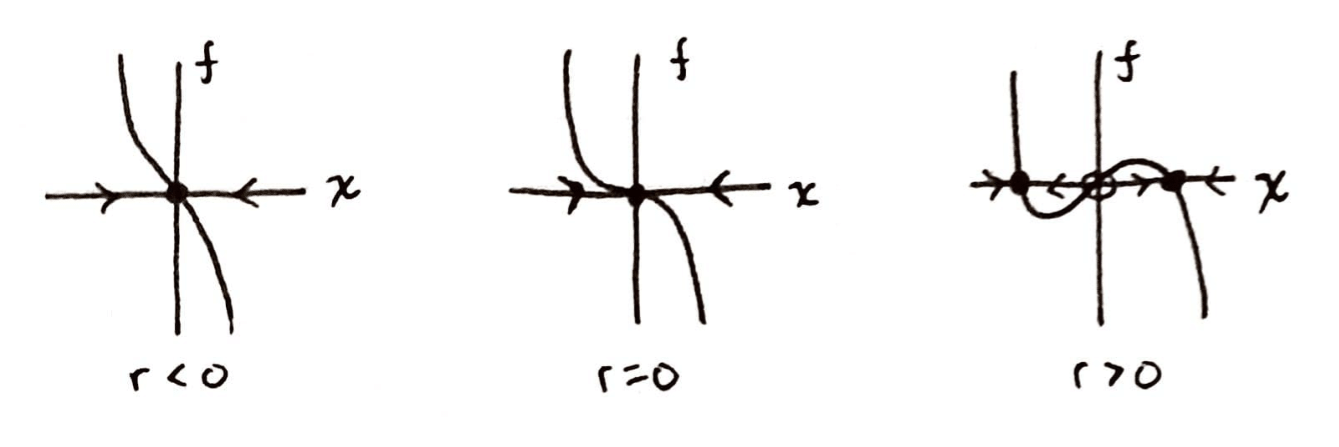
\includegraphics[height=0.2\textwidth]{img/2020F1a1.png}
    \end{center}
    We see that the fixed point $x = 0$ is stable for $r \leq 0$ and unstable for $r \geq 0$, and that the fixed points $r = x^2$, which come into existence for $r \geq 0$, are stable. So, we get the following bifurcation diagram for $a = 0$:
    \begin{center}
        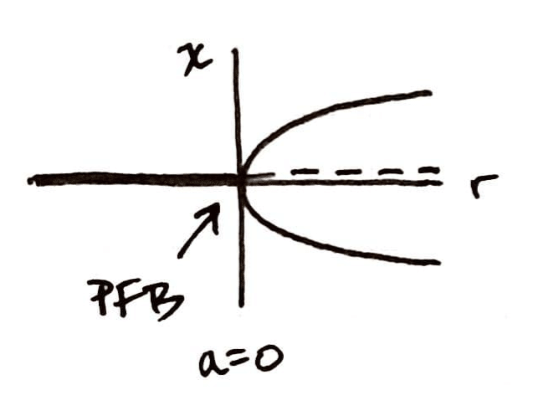
\includegraphics[height=0.2\textwidth]{img/2020F1a2.png}
    \end{center}
    A supercritical pitchfork bifurcation occurs at the point $(r, x) = (0, 0)$.
    
    When $a \ne 0$, the global stability behavior of the system remains unchanged, so the behavior of our system should only be a mild perturbation of the behavior of the case $a = 0$. Although the exact values of our fixed points change, the broad image of their stability does not. So, we get the following bifurcation diagrams, for $a < 0$ and $a > 0$, respectively:
    \begin{center}
        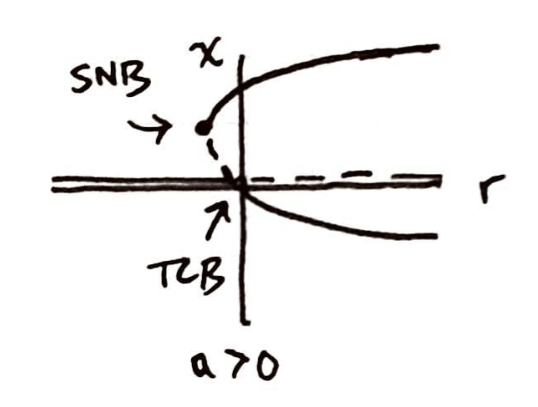
\includegraphics[height=0.2\textwidth]{img/2020F1a3.png}
        \qquad
        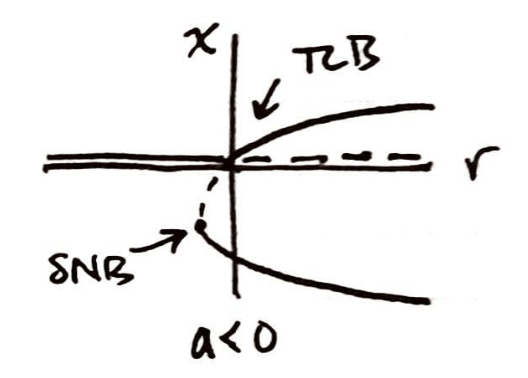
\includegraphics[height=0.2\textwidth]{img/2020F1a4.png}
    \end{center}
    In each of these situations, the pitchfork bifurcation from the $a = 0$ case splits into two separate bifurcations: a saddle-node bifurcation and a transcritical bifurcation. The transcritical bifurcation occurs at $(r, x) = (0, 0)$, while the saddle-node bifurcation occurs where the fixed point $r = x(x- a) = x^2 - ax$ comes into existence:
    \begin{align*}
    x^2 - ax - r &= 0
    \so
    x = \frac{1}{2}\left(a \pm \sqrt{a^2 + 4r}\right) \so
    r = -\frac{a^2}{4}
    \end{align*}
    So, the saddle-node bifurcation occurs at $(r, x) = \left(-a^2/4,\ a/2\right)$.
    
    
    \item The fixed points of the system are $x = 0$ and $x = \frac{1}{2}\left(a \pm \sqrt{a^2 + 4r}\right)$. Note the regions of existence:
    \[
    x = \frac{1}{2}\left(a \pm \sqrt{a^2 + 4r}\right) = \begin{cases}
    \textrm{DNE} &: a^2 + 4r < 0
    \\
    1 \textrm{ FP} &: a^2 + 4r = 0
    \\
    2 \textrm{ FPs} &: a^2 + 4r > 0
    \end{cases}
    \]
    So, we have saddle-node bifurcations along the line $a^2 + 4r = 0$. We also get transcritical bifurcations wherever either of these fixed points collide with the point $x = 0:$
    \begin{align*}
        0 &= \frac{1}{2}\left(a \pm \sqrt{a^2 + 4r}\right)
        \\
        a &= \mp \sqrt{a^2 + 4r}
        \\
        a^2 &= a^2 + 4r \\
        r &= 0
    \end{align*}
    So, we have transcritcal bifurcations along the line $r = 0$. Altogether, this means we also get a pitchfork bifurcation where these two bifurcations collide, at $r = a = 0$. So, we get the following $(r, a)$ plot:
    
    \begin{center}
        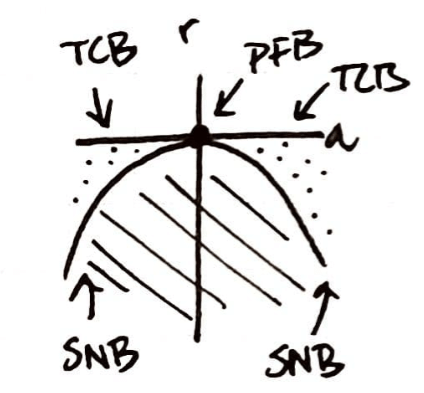
\includegraphics[height=0.25\textwidth]{img/2020F1b.png}
    \end{center}
\end{enumerate}

\item \begin{qbox}
Consider the system of equations 
\begin{align*}
    \frac{dx}{dt} &= \lambda x - y - xr^2 + \lambda \frac{x^3}{r} \\
    \frac{dy}{dt} &= x + \lambda y - yr^2 + \lambda \frac{x^2 y}{r}
\end{align*}
where $r$ is the polar radius, i.e., $r^2 = x^2 + y^2$. Show that this system has a stable limit cycle when $\lambda > 0$.
\end{qbox}

We begin by converting our system of equations to polar coordinates. We begin with the equation for $\dot r:$
\begin{align*}
    r \dot r &= x \dot x + y \dot y \\
    r \dot r &= x\left(\lambda x - y - xr^2 + \lambda \frac{x^3}{r}\right) + y\left(x + \lambda y - yr^2 + \lambda \frac{x^2 y}{r}\right)
    \\
    r \dot r &= \lambda x^2 - xy - x^2r^2 + \lambda \frac{x^4}{r} + xy + \lambda y^2 - y^2r^2 + \lambda \frac{x^2 y^2}{r}
    \\
    r \dot r &= \lambda r^2 - r^4 + \frac \lambda  r \left( x^2 r^2\right)
    \\
    \dot r &= \lambda r - r^3 + \lambda x^2
\end{align*}
Next, we find the equation for $\dot \theta:$
\begin{align*}
    r^2 \dot \theta &= x\dot y - y \dot x
    \\
    r^2 \dot \theta &= x\left(x + \lambda y - yr^2 + \lambda \frac{x^2 y}{r}\right) - y\left(\lambda x - y - xr^2 + \lambda \frac{x^3}{r}\right)
    \\
    r^2 \dot \theta &= x^2 + \lambda xy - xyr^2 + \lambda \frac{x^3 y}{r} - \left(\lambda xy - y^2 - xyr^2 + \lambda \frac{x^3y}{r}\right)
    \\
    r^2 \dot \theta &= x^2 + y^2
    \\
    r^2 \dot \theta &= r^2 \\
    \dot \theta &= 1 \qquad (r \ne 0)
\end{align*}
So, our system of equations is given in polar coordinates by
\[
\begin{cases}
\dot r = \lambda r - r^3 + \lambda x^2
\\
\dot \theta = 1.
\end{cases}
\]
We examine the region in which $r$ is decreasing, that is, $\dot r < 0$. Note that since $\lambda > 0$,
\begin{align*}
    \dot r &=
    \lambda r - r^3 + \lambda x^2 
    \leq \lambda r - r^3 + \lambda \left(x^2 + y^2\right) 
    = \lambda r - r^3 + \lambda r^2.
\end{align*}
There will always exist some $r > 0$ such that the $-r^3$ term dominates. Label such a satisfactory $r$ by $R$. So,
\[
\dot r\ \big \vert_{r = R} \leq \lambda R - R^3 + \lambda R^2 < 0.
\]
In the phase plane, flow points inward along the circle $r = R$. Now, we examine the region in which $r$ is increasing. Note that
\[
\dot r = \lambda r - r^3 + \lambda x^2 \geq \lambda r - r^3 = r\left(\lambda - r^2\right)
\]
When $r > 0$, this value is positive if $\lambda > r^2$, that is, if $0 < r < \sqrt{ \lambda}$. Label such a satisfactory $r$ by $\widetilde{r}$. So,
\[
\dot r\ \big \vert_{r = \widetilde{r}} \geq \widetilde{r}\left(\lambda - \widetilde{r}^2\right) > 0.
\]
In the phase plane, flow points outward along the circle $r = \widetilde{r}$. 

Note that $R$ could be chosen to be arbitrarily large, so long as it is large \textit{enough} that $\dot r\ \big \vert_{r = R} < 0$. So, we choose it large enough such that $R > \widetilde{r}$ as well. Then, we have a trapping region: $0 < \widetilde{r} \leq r \leq R$. 

By the Poincar\'e-Bendixon theorem, if our system is continuously differentiable over the trapping region, if the region is closed and bounded, and if the region contains no fixed points, then it must contain a closed orbit. The region $\widetilde{r} \leq r \leq R$ is closed and bounded and our system is indeed continuously differentiable in this region. Our conversion to polar coordinates showed that the only fixed point of our system is at $r = 0$, and so our trapping region contains no fixed points. Therefore, we have a closed orbit in this region. Since flow points into our trapping region rather than out of it, this limit cycle is stable.




\item \begin{qbox}
Let
\[
\mathcal{E}\big[y(x)\big] = \int_0^1 \left[\frac{d^2y}{dx^2}\right]^2\,dx.
\]
Derive the equation for $y(x)$ which extremizes $\mathcal{E}$ subject to the constraint
\[
\int_0^1 \big[y(x)\big]^2\,dx = 1
\]
and the boundary conditions $y(0) = y(1) = y'(0) = y'(1) = 0$, where $y' = dy/dx$. Find the functions which extremize $\mathcal E$. What would be considered the natural boundary conditions for this problem?
\end{qbox}

We use the method of Lagrange multipliers. Let $f = (y'')^2$ and $g = y^2$, then define $h = f + \lambda g = (y'')^2 + \lambda y^2$. The Euler-Lagrange equation is then
\[
\pp{h}{y} - \frac{d}{dx}\pp{h}{y'} + \frac{d^2}{dx^2}\pp{h}{y''} = 0.
\]
We compute each of the components of the Euler-Lagrange equation.
\begin{align*}
    \pp{h}{y} &= 2\lambda y \\
    \pp{h}{y'} &= 0 \\
    \frac{d^2}{dx^2}\pp{h}{y''} &= \frac{d^2}{dx^2}(2y'') = 2y^{(4)}.
\end{align*}
So, our Euler-Lagrange equation becomes
\[
y^{(4)} + \lambda y = 0.
\]
Now, we find the sign of $\lambda$. We multiply our equation by $y$ and integrate:
\begin{align*}
    \int_0^1 yy^{(4)}\,dx &= - \lambda \int_0^1  y^2\,dx
    \\
    y y^{(3)} \big\vert_0^1 - \int_0^1y'y^{(3)}\,dx &= - \lambda \int  y^2\,dx 
    &\textrm{(IBP)}
    \\
    y y^{(3)} \big\vert_0^1 - y'y''\big\vert_0^1 + \int_0^1(y'')^2\,dx &= - \lambda \int  y^2\,dx 
    &\textrm{(IBP again)}
    \\
    \int_0^1(y'')^2\,dx &= - \lambda \int y^2\,dx 
    &\textrm{(boundary terms vanish)}
\end{align*}
Since both of our integrals are nonnegative, we must have $-\lambda \geq 0$, and so $\lambda \leq 0$. So, we label $\lambda = -\mu^4$ for convenience. Our equation now has the form
\[
y^{(4)} - \mu^4 y = 0,
\]
which has solutions of the form
\begin{align*}
y &= A e^{\mu x} + B e^{-\mu x} + Ce^{i\mu x} + D e^{-i\mu x} \\
y' &= \mu\left(A e^{\mu x} - B e^{-\mu x} + i C e^{i\mu x} -i D e^{-i\mu x}\right)
\end{align*}
Our boundary conditions become
\begin{align*}
    A + B + D &= 0 \\
    A - B + C &= 0 \\
    A e^{\mu} + Be^{-\mu} + C\sin(\mu) + D\cos(\mu) &= 0 \\
    Ae^\mu - Be^{-\mu} + C\cos(\mu) - D\sin(\mu) &= 0
\end{align*}
So, a satisfactory $y(x)$ would have $A, B, C, D$ that satisfy the above conditions, and we then would solve for the value of $\mu$ by plugging the resulting equation $y(x; \mu)$ into the integral constraint
\[
\int_0^1 \big[y(x)\big]^2 = 1.
\]
Now, if we wish to extremize $\mathcal{E}$ in the general case (not subject to the given integral constraint), we have the Euler-Lagrange equation 
\begin{align*}
\pp{f}{y} - \frac{d}{dx}\pp{f}{y'} + \frac{d^2}{dx^2}\pp{f}{y''} &= 0
\so y^{(4)} = 0.
\end{align*}
This equation has solutions of the form
\[
y(x) = Ax^3 + Bx^2 + Cx + D.
\]
Now we need to find the natural boundary conditions. In the general case, in the derivation of the Euler-Lagrange equation of the variational problem 
\[
\int_{0}^{1}f(x, y, y', y'')dx \to \min/\max,
\]
we perform a one-parameter variation of $y = \bar y(x, \epsilon)$ from the solution $\bar y(x)$. Defining
\[
\eta(x, \epsilon) = \frac{\partial \bar y(x, \epsilon)}{\partial \epsilon} \qquad \textrm{and} \qquad \eta'(x, \epsilon) = \frac{\partial \bar y'(x, \epsilon)}{\partial \epsilon},
\]
and differentiating the integral 
\[
I(\epsilon) = \int_{0}^{1}f(x, \bar y(x, \epsilon), \bar y'(x, \epsilon), \bar y''(x, \epsilon))\,dx,
\]
with respect to $\epsilon$, we wish to arrive at
\[
\frac{dI(\epsilon)}{d\epsilon} = \int_{0}^{1}\frac{\partial f}{\partial y}\eta\,dx + \int_{0}^{1}\frac{\partial f}{\partial y'}\eta'\,dx + \int_{0}^{1}\frac{\partial f}{\partial y''}\eta''\,dx = 0.
\]
When we perform integration by parts on the two rightmost integrals, the following boundary terms pop out:
\begin{align*}
    (1): &\quad \eta \left(\pp{f}{y'} - \frac{d}{dx}\frac{\partial f}{\partial y''}\right)\bigg\vert_{0}^1  \qquad \qquad
    (2): \quad \eta'\frac{\partial f}{\partial y''}\bigg\vert_{0}^{1}
\end{align*}
We must set both of these terms equal to zero regardless of $\eta$, and so the natural boundary conditions in the general case are 
\begin{align*}
    \left(\pp{f}{y'} - \frac{d}{dx}\frac{\partial f}{\partial y''}\right)\bigg\vert_{x = 0, 1} = 0 \qquad \textrm{and} \qquad
    \frac{\partial f}{\partial y''}\bigg\vert_{x = 0, 1} = 0.
\end{align*}
For this particular problem, since $f = (y'')^2$, the natural boundary conditions are therefore
\begin{align*}
    y'''(0) = 0, \quad y'''(1) = 0, \quad y''(0) = 0, \quad y''(1) = 0.
\end{align*}


\item \begin{qbox}
Find the solution $G(x, \xi)$ (the Green's function) to the problem
\[
\frac{d^2G}{dx^2} - G = \delta(x - \xi)
\]
with $G(0,\xi) = G(L, \xi) = 0$. Use the Green's function to compute the solution of
\[
\frac{d^2y}{dx^2} - y = H(x)
\]
with $y(0) = y(L) = 0$, and 
\[
H(x) = \begin{cases}
0 &: 0 \leq x \leq \frac L 2 \\
1 &: \frac L 2 < x \leq L
\end{cases}
\]
\end{qbox}
The homogenous version of our equation is
\[
y''(x) - y(x) = 0,
\]
which has solutions of the form
\[
y = Ae^x + Be^{-x}.
\]
Plugging in the left boundary condition $y(0) = 0$ gives $A + B = 0$, and so our first equation is
\[
y_1 = e^x - e^{-x}.
\]
The boundary condition $y(L) = 0$ gives $Ae^L + Be^{-L} = 0$, and so we get $A = -B e^{-2L}$. So, our second equation is
\[
y_2 = e^{-x} - e^{x-2L}.
\]
So, our Green's function has the form
\[
G(x, \xi) = \begin{cases}
\frac{1}{c}y_1(x)y_2(\xi) &: x \leq \xi
\\
\frac{1}{c}y_1(\xi)y_2(x) &: x \geq \xi
\end{cases}
\]
Here, $c = pw$, where $p = 1$ in this problem and $w$ is the Wronskian:
\begin{align*}
    w &= \det \mtx{cc}{y_1 & y_2 \\ y_1' & y_2'}
    =
    \det \mtx{cc}{e^x - e^{-x} & e^{-x} - e^{x-2L} \\ e^x + e^{-x} & -e^{-x} - e^{x-2L}}
    =
    -2 + 2e^{-2L}.
\end{align*}
So, our green's function is
\[
G(x, \xi) = \begin{cases}
\frac{1}{c}\left(e^{x} - e^{-x}\right)\left(e^{-\xi} - e^{\xi-2L}\right) &: x \leq \xi
\\
\frac{1}{c}\left(e^{\xi} - e^{-\xi}\right)\left(e^{-x} - e^{x-2L}\right) &: x \geq \xi
\end{cases}
\]
where $c = \left(-2 + 2e^{-2L}\right)^{-1}$ as given above.

The solution of the given problem for $x \geq L/2$ is
\begin{align*}
    y_A(x) &= \int_0^L G(x;\xi)H(\xi)\,d\xi
    \\
    &=
    \int_{L/2}^L G(x;\xi)\,d\xi
    \\
    &=
    \int_{L/2}^x G(x;\xi)\,d\xi + \int_{x}^L G(x;\xi)\,d\xi
    \\
    &=
    \frac{1}{c}\left(e^{-x} - e^{x-2L}\right)\int_{L/2}^x \left(e^{\xi} - e^{-\xi}\right)\,d\xi
    +
    \frac{1}{c}\left(e^{x} - e^{-x}\right)\int_{x}^L\left(e^{-\xi} - e^{\xi-2L}\right)\,d\xi
    \\
    &= \frac{1}{c}\left[\left(e^{-x} - e^{x-2L}\right)\left(-e^{-L/2} - e^{L/2} + e^{-x} + e^x\right) + \left(e^{x} - e^{-x}\right)\left(-2 e^{-L} + e^{-x} + e^{-2 L + x}\right) \right]
\end{align*}
For $x \leq L/2$, we get
\begin{align*}
    y_B(x) &= \int_0^L G(x;\xi)H(\xi)\,d\xi
    \\
    &=
    \int_{L/2}^L G(x;\xi)\,d\xi
    \\
    &=
    \frac{1}{c}\left(e^{x} - e^{-x}\right) \int_{L/2}^L \left(e^{-\xi} - e^{\xi-2L}\right) \,d\xi
    \\
    &=
    \frac{1}{c}\left(e^{x} - e^{-x}\right)\left(e^{-3 L/2} - 2 e^{-L} + e^{-L/2}\right)
\end{align*}
So, we have
\[
y = \begin{cases}
y_B(x) &: 0 \leq x \leq \frac{L}{2} \\
y_A(x) &: \frac{L}{2} \leq x \leq L
\end{cases}
\]


\item \begin{qbox}
A simple harmonic oscillator is subject to weak nonlinear damping proportional to the square of its velocity, and its displacement $y(t; \epsilon)$ satisfies the nondimensionalized initial value problem
\[
\frac{d^2y}{dt^2} + \epsilon\frac{dy}{dt}\abs{\frac{dy}{dt}} + y = 0, \qquad y(0;\epsilon) = 1, \qquad \frac{dy}{dt}(0;\epsilon) = 0.
\]
Use the method of multiple scales to find a leading order approximation for $y(t; \epsilon)$ as $\epsilon\to 0^+$, valid on times $t = \Ord{\epsilon^{-1}}$.

\textit{Hint:} The function $\sin t|\sin t|$ has the Fourier expansion
\[
\sin t \abs{\sin t} = \sum_{n = 1}^\infty b_n \sin nt, \qquad b_1 = \frac{8}{3\pi}.
\]
\end{qbox}

Since our expansion must be valid on times $t = \Ord{\epsilon^{-1}}$, we set $t_1 = t$ and $t_2 = \epsilon t$. If $y = y(t_1, t_2)$, then our equation becomes
\[
\left(\partial_{t_1}^2 + \epsilon2\partial_{t_1t_2} + \epsilon^2 \partial^2_{t_2}\right)y + \epsilon\left(\partial_{t_1} + \epsilon\partial_{t_2}\right)y\cdot \abs{\left(\partial_{t_1} + \epsilon\partial_{t_2}\right)y} + y = 0
\]
with initial conditions
\begin{align*}
    y(0, 0) = 1, \qquad \left(\partial_{t_1} + \epsilon\partial_{t_2}\right)y\big\vert_{0,0} = 0.
\end{align*}
Our leading-order $\Ord{1}$ equation is
\[
\partial_{t_1}^2 y_0 + y_0 = 0
\]
which yields the solution
\begin{align*}
    y_0 &= \phantom{-}A(t_2)\cos(t_1 + \theta(t_2)) \\
    \partial_{t_1} y_0 &= -A(t_2)\sin(t_1 + \theta(t_2))
\end{align*}
Plugging in our initial conditions yields
\[
A(0)\cos(\theta(0)) = 1, \qquad A(0)\sin(\theta(0)) = 0.
\]
Note that our first condition gives that $A(0) \ne 0$, and so our second condition therefore yields $\theta(0) = k\pi$ for some $k \in \Z$. In turn, our first equation then becomes $A(0) = (-1)^k$.

Now, we move on to the $\Ord \epsilon$ equation:
\begin{align*}
    \partial_{t_1}^2 y_1 + 2\partial_{t_1t_2}y_0 + \partial_{t_1}y_0\abs{\partial_{t_1}y_0} + y_1 &= 0
\end{align*}
We examine the $y_0$ terms to find secular terms:
\begin{align*}
    \partial_{t_1t_2}y_0 &= -A'(t_2)\sin(t_1 + \theta(t_2)) - A(t_2)\theta'(t_2)\cos(t_1+\theta(t_2)) 
    \\ \\
    \partial_{t_1}y_0\abs{\partial_{t_1}y_0}
    &=
    -A(t_2)\sin(t_1 + \theta(t_2))\abs{A(t_2)\sin(t_1 + \theta(t_2))}
    \\
    &= -A(t_2)\abs{A(t_2)}\cdot \sin(t_1 + \theta(t_2))\abs{\sin(t_1 + \theta(t_2))}
    \\
    &= -A(t_2)\abs{A(t_2)}\cdot \sum_{n=1}^\infty \sin(nt_1 + n\theta(t_2))
    \\
    &=-A(t_2)\abs{A(t_2)}\cdot \frac{8}{3\pi}\sin(t_1 + \theta(t_2)) + \textrm{[nonsecular terms]}
\end{align*}
So, our $\Ord \epsilon$ equation can now be written as
\begin{align*}
    \partial_{t_1}^2 y_1 + y_1 &= \left(2A'(t_2) + \frac{8}{3\pi}A(t_2)\abs{A(t_2)}\right)\sin(t_1 + \theta(t_2)) + 2A(t_2)\theta'(t_2)\cos(t_1 + \theta(t_2)) + \textrm{[nonsec terms]}
\end{align*}
So, in order to eliminate secular terms, we require
\[
2A'(t_2) + \frac{8}{3\pi}A(t_2)\abs{A(t_2)} = 0 \qquad \textrm{and} \qquad A(t_2)\theta'(t_2) = 0.
\]
Recall that our initial conditions are $\theta(0) = k\pi$ for some $k \in \Z$, and $A(0) = (-1)^k$, dependent on $\theta$. Therefore $A(t_2) \ne 0$, and so
\[
A(t_2)\theta'(t_2) = 0 \so \theta'(t_2) = 0 \so \theta(t_2) = k\pi, \quad k \in \Z.
\]
Now, we solve for $A:$
\begin{align*}
    2A'(t_2) + \frac{8}{3\pi}A(t_2)\abs{A(t_2)} &= 0
    \\
    -A'(t_2) &= \frac{4}{3\pi}A(t_2)\abs{A(t_2)} \\
    -\frac{A'(t_2)}{A(t_2)\abs{A(t_2)}} &= \frac{8}{3\pi}
    \\
    -\sgn(A)\int\frac{dA}{A^2} &= \int\frac{4}{3\pi}\,dt_2
    \\
    \sgn(A)\cdot \frac{1}{A} &= \frac{4}{3\pi}t_2 + C
    \\
    \frac{1}{\abs{A}} &= \frac{4}{3\pi}t_2 + C
    \\
    \abs{A(t_2)} &= \frac{1}{\frac{4}{3\pi}t_2 + C}
    \\
    \abs{A(t_2)} &= \frac{3\pi}{4t_2 + 3\pi \cdot C}
\end{align*}
Plugging in $A(0) = (-1)^k$, or $\abs{A(0)} = 1$, this becomes
\[
1 = \frac{1}{C} \so C = 1.
\]
So, if we assume that $A = (-1)^k \abs{A}$, then
\[
\abs{A(t_2)} = \frac{3\pi}{3\pi + 4t_2} \so A(t_2) = (-1)^k\frac{3\pi}{3\pi + 4t_2}
\]
So, our approximation for $y$ would be
\begin{align*}
    y &\thicksim A(t_2)\cos(t_1 + \theta(t_2))
    = \frac{3\pi }{3\pi + 4\epsilon t}(-1)^k\cos(t + k\pi)
    = \frac{3\pi }{3\pi + 4\epsilon t}(-1)^{2k}\cos t
    = \frac{3\pi}{3\pi + 4\epsilon t}\cos t.
\end{align*}

\item \begin{qbox}
Use the method of matched asymptotic expansions to find a leading-order approximation for the solution $y(x; \epsilon)$ of the following boundary value problem on $0 \leq x \leq 1:$
\[
\epsilon y'' + 2y' + y^3 = 0, \qquad y(0; \epsilon) = 0, \quad y(1, \epsilon) = \frac{1}{2}.
\]
\end{qbox}
First, we examine the $\Ord 1$ equation:
\begin{align*}
    2y' + y^3 &= 0 \\
    \int \frac{dy}{y^3} &= -\int \frac{1}{2}\,dx \\
    -\frac{1}{2}y^{-2} &= -\frac{1}{2}x + C
    \\
    y^{-2} &= x + C \\
    y^{-1} &= \pm \sqrt{x + C} \\
    y &= \frac{\pm 1}{\sqrt{x + C}}
\end{align*}
Since the coefficent of our $y'$ term in our equation is positive, we expect a boundary layer at $x = 0$. So, we apply the boundary condition $y(1) = 1/2$ to the leading-order expansion to get
\[
\frac{1}{2} = \pm \frac{1}{\sqrt{1 + C}} \so 2 = \sqrt{1 + C} \so C = 3.
\]
So, our outer solution is given by
\[
y_{out} = \frac{1}{\sqrt{x + 3}}.
\]
Now, we rescale $x$ to find the inner solution. We define $\hat x = x/\epsilon$. Then, our equation becomes 
\[
\epsilon^{-1} y'' + 2\epsilon^{-1} y' + y^3 = 0.
\]
Examining the $\Ord{\epsilon^{-1}}$ equation, we get
\begin{align*}
    y'' + 2y' &= 0 \\
    y' &= A e^{-2\hat x} \\
    y &= A e^{-2 \hat x} + B
\end{align*}
Applying the boundary condition $y(0) = 0$, we get
\[
0 = A + B \so B = -A.
\]
So, our inner solution is given by
\[
y_{in} = A e^{-2 \hat x} - A.
\]
Now, we match our inner and outer solutions.
\begin{align*}
    \lim_{x \to 0} y_{out} &= \lim_{x\to 0} \frac{1}{\sqrt{x + 3}} = \frac{1}{\sqrt 3} \\
    \lim_{\hat x \to \infty} y_{in} &= \lim_{\hat x \to \infty} \left[A e^{-2 \hat x} - A\right] = -A.
\end{align*}
So, we set $A = -1/\sqrt 3$, and so $y_{overlap} = 1/\sqrt 3$. Our composite solution is given by $y_{out} + y_{in} - y_{overlap}:$
\[
y \thicksim \frac{1}{\sqrt{x + 3}} - \frac{1}{\sqrt 3} e^{-2 x / \epsilon}.
\]
\end{enumerate}

\chapter*{Fall 2019}
\chaptermark{Fall 2019}
\addcontentsline{toc}{chapter}{Fall 2019}

\begin{enumerate}
    \item 
    \begin{qbox}
    Consider the planar system
    \[
    \frac{dx}{dt} = x(1 - x - y), \qquad \frac{dy}{dt} = y\left(3 - x - \frac{3}{2}y\right).
    \]
    \begin{itemize}
        \item[(a)] Give an interpretation of this system in terms of the population dynamics of species $x(t) \geq 0,\ y(t) \geq 0$.
        \item[(b)] Find the equilibria with $x, y \geq 0$, determine their linearized stability, and classify them.
        \item[(c)] Sketch the phase plane of the system in $x \geq 0,\ y \geq 0$.
        \item[(d)] Suppose that $x(0), y(0) > 0$. What happens to the solution as $t \to +\infty$? What is the interpretation in terms of population dynamics?
    \end{itemize}
    \end{qbox}
    
    \begin{enumerate}
        \item This system describes two species which are competing against each other for the same resources.
        
        \item We set $\dot x$ and $\dot y$ equal to zero and solve for our equilibria:
        \begin{alignat*}{6}
            \dot x &= x(1 - x - y) = 0 
            &\qquad& \rightarrow &\qquad& 
            x &= 0 &\quad& \textrm{or} &\quad& y &= 1 - x 
            \\
            \dot y &= y\left(3 - x - \frac{3}{2}y\right) = 0 
            &\qquad& \rightarrow &\qquad& 
            y &= 0 &\quad& \textrm{or} &\quad& y &= 2 - \frac{2}{3}x
        \end{alignat*}
        We sketch our curves in the first quadrant to see their intersections:
        \begin{center}
        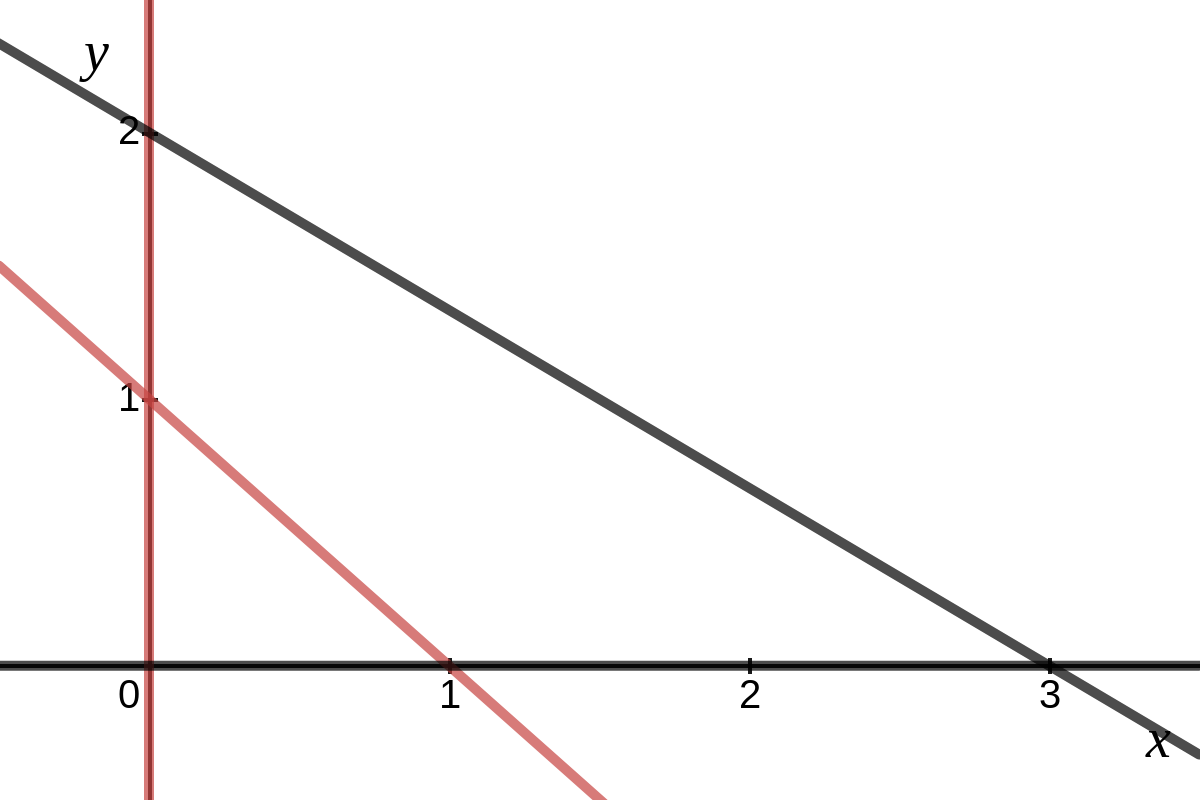
\includegraphics[height=0.3\textwidth]{img/2019F1a.png}
        \end{center}
        Only the places where the red and black lines overlap are possible equilibria. So, are equilibria are
        \[
        (x, y) = (0, 0), (1, 0), \textrm{ and } (0, 2).
        \]
        To determine their linearized stability, we compute the Jacobian:
        \[
        J = \mtx{cc}{
        -2x + 1 - y & -x \\ 
        -y & 3 - x - 3y
        }
        \]
        We plug in each of our equilibria and examine the eigenvalues.
        \begin{alignat*}{3}
            J\big\vert_{(0, 0)} &= \mtx{cc}{1 & 0 \\ 0 & 3} \qquad &\rightarrow \qquad \lambda &= 1, 3 \qquad &\rightarrow& \qquad \textrm{Unstable Node}
            \\
            J\big\vert_{(1, 0)} &= \mtx{rr}{-1 & -1 \\ 0 & 2} \qquad &\rightarrow \qquad \lambda &= -1, 2 \qquad &\rightarrow& \qquad \textrm{Saddle (Unstable)}
            \\
            J\big\vert_{(0, 2)} &= \mtx{cc}{-1 & 0 \\ -2 & -3} \qquad &\rightarrow \qquad \lambda &= -2, -3 \qquad &\rightarrow& \qquad \textrm{Stable Node}
        \end{alignat*}
        
        \item \ 
        \begin{center}
        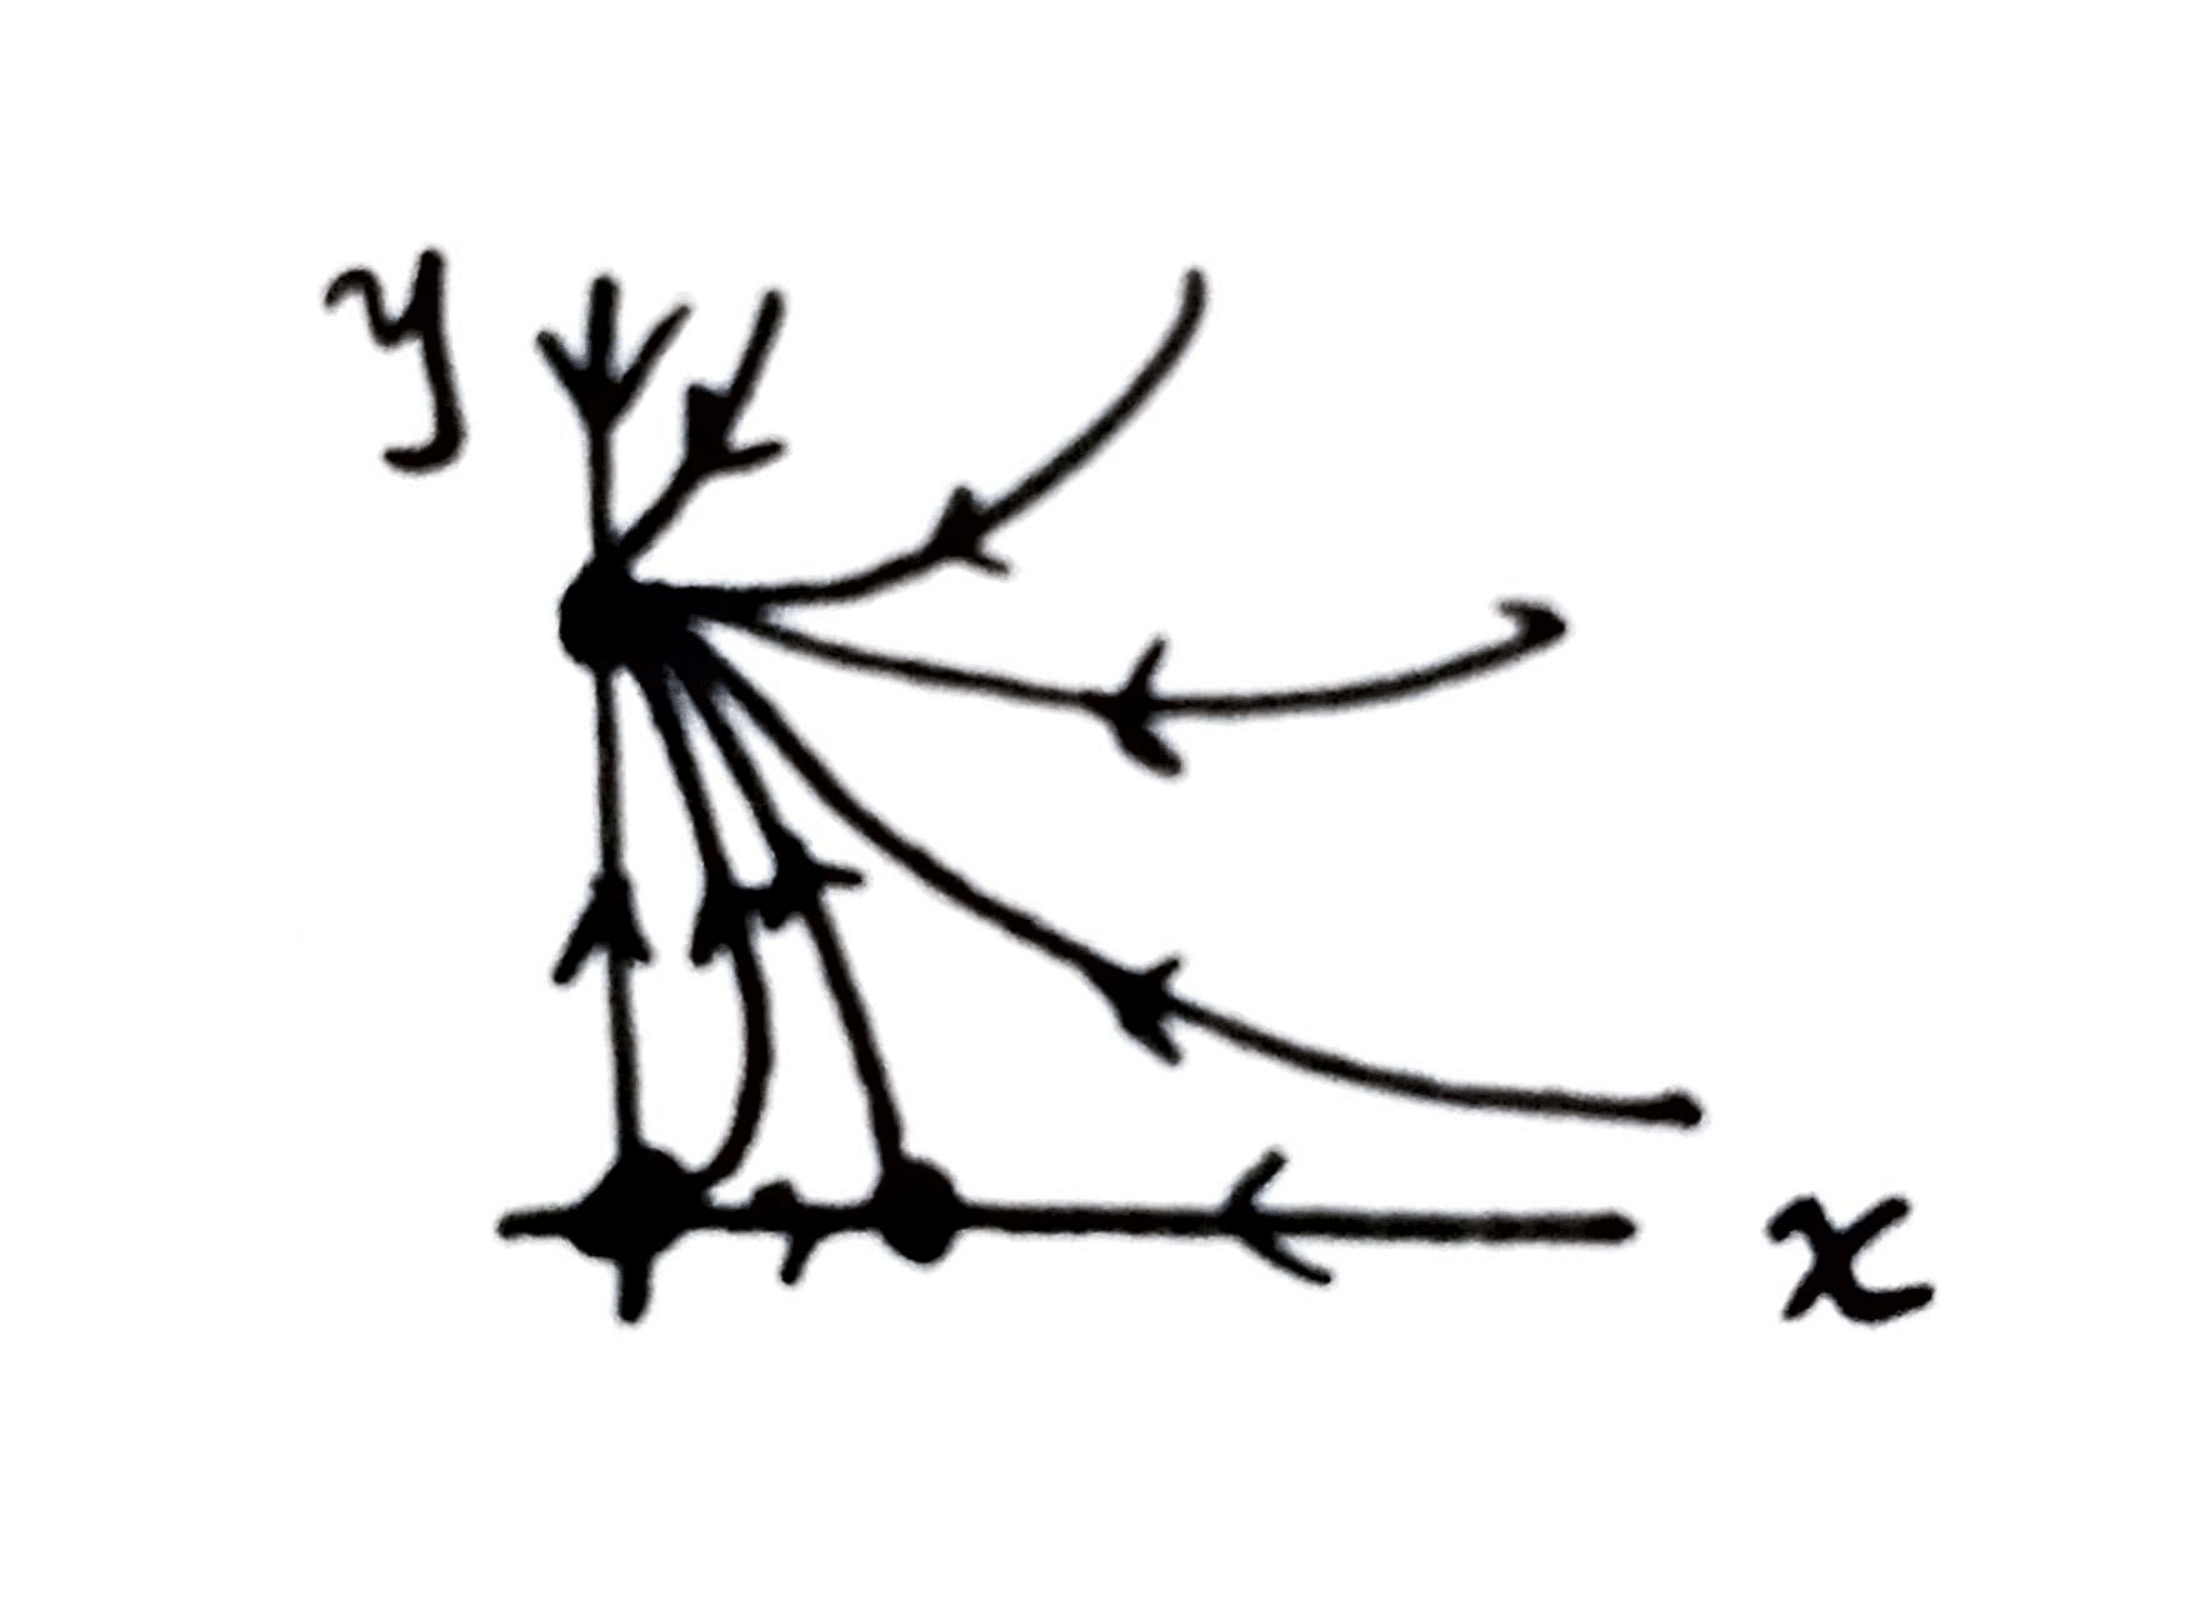
\includegraphics[height=0.25\textwidth]{img/2019F1c.png}
        \end{center}
        
        \item As $t\to+\infty$, our system tends toward the equilibrium $(x, y) = (0, 2)$. Biologically, this means species $y$ dominates and species $x$ dies out.
    \end{enumerate}
    
    \item 
    \begin{qbox}
    A discrete dynamical system for $x_n \in \R$ with $n = 0, 1, 2, \ldots$ depending on a parameter $\mu \in \R$ is given by
    \[ x_{n+1} = x_n^2 + \mu.\]
    \begin{itemize}
        \item[(a)] Find the fixed points of the system and determine their linearized stability. Sketch a bifurcation diagram for the fixed points, indicating stable fixed points by a solid line and unstable fixed points by a dashed line.
        \item[(b)] What types of bifurcations occur at the fixed points as $\mu$ increases from $-\infty$ to $\infty$?
    \end{itemize}
    \end{qbox}
    
    \begin{enumerate}
        \item To find the fixed points, we set $x_{n} = x_{n + 1} = \widetilde x$ and solve for $\widetilde x$:
        \begin{align*}
            \widetilde{x} &= \widetilde x ^2 + \mu
            \\
            \widetilde x^2 - \widetilde x + \mu &= 0
            \\
            &\Downarrow
            \\
            \widetilde x &= \frac{1}{2}\pm \frac{1}{2}\sqrt{1 - 4\mu}, \quad \textrm{(exists for $\mu < 1/4$.)}
        \end{align*}
        If $f(x) = x^2 + \mu$, then we determine the linearized stability of these fixed points by plugging in $\widetilde x$ to $f'(x) = 2x$:
        \begin{align*}
        f'(\widetilde x_{+}) 
        &= 
        1 + \sqrt{1 - 4\mu}
        \\
        f'(\widetilde x_{-}) 
        &= 
        1 - \sqrt{1 - 4\mu}
        \end{align*}
        Since $\abs{f'(\widetilde x_+)} > 1$ everywhere the equilibrium exists (all $\mu < 1/4$), $\widetilde x_{+}$ is \textbf{always unstable}.
        
        On the other hand, $f'(\widetilde x_-)$ is smaller than 1 in magnitude for $\mu > -3/4$, but for $\mu < -3/4$, we have $f'(\widetilde x_-) < -1$. So, $\widetilde x_-$ is \textbf{unstable} for $\mu < -3/4$ and \textbf{stable} for $-3/4 < \mu < 1/4$.
    
        \begin{center}
        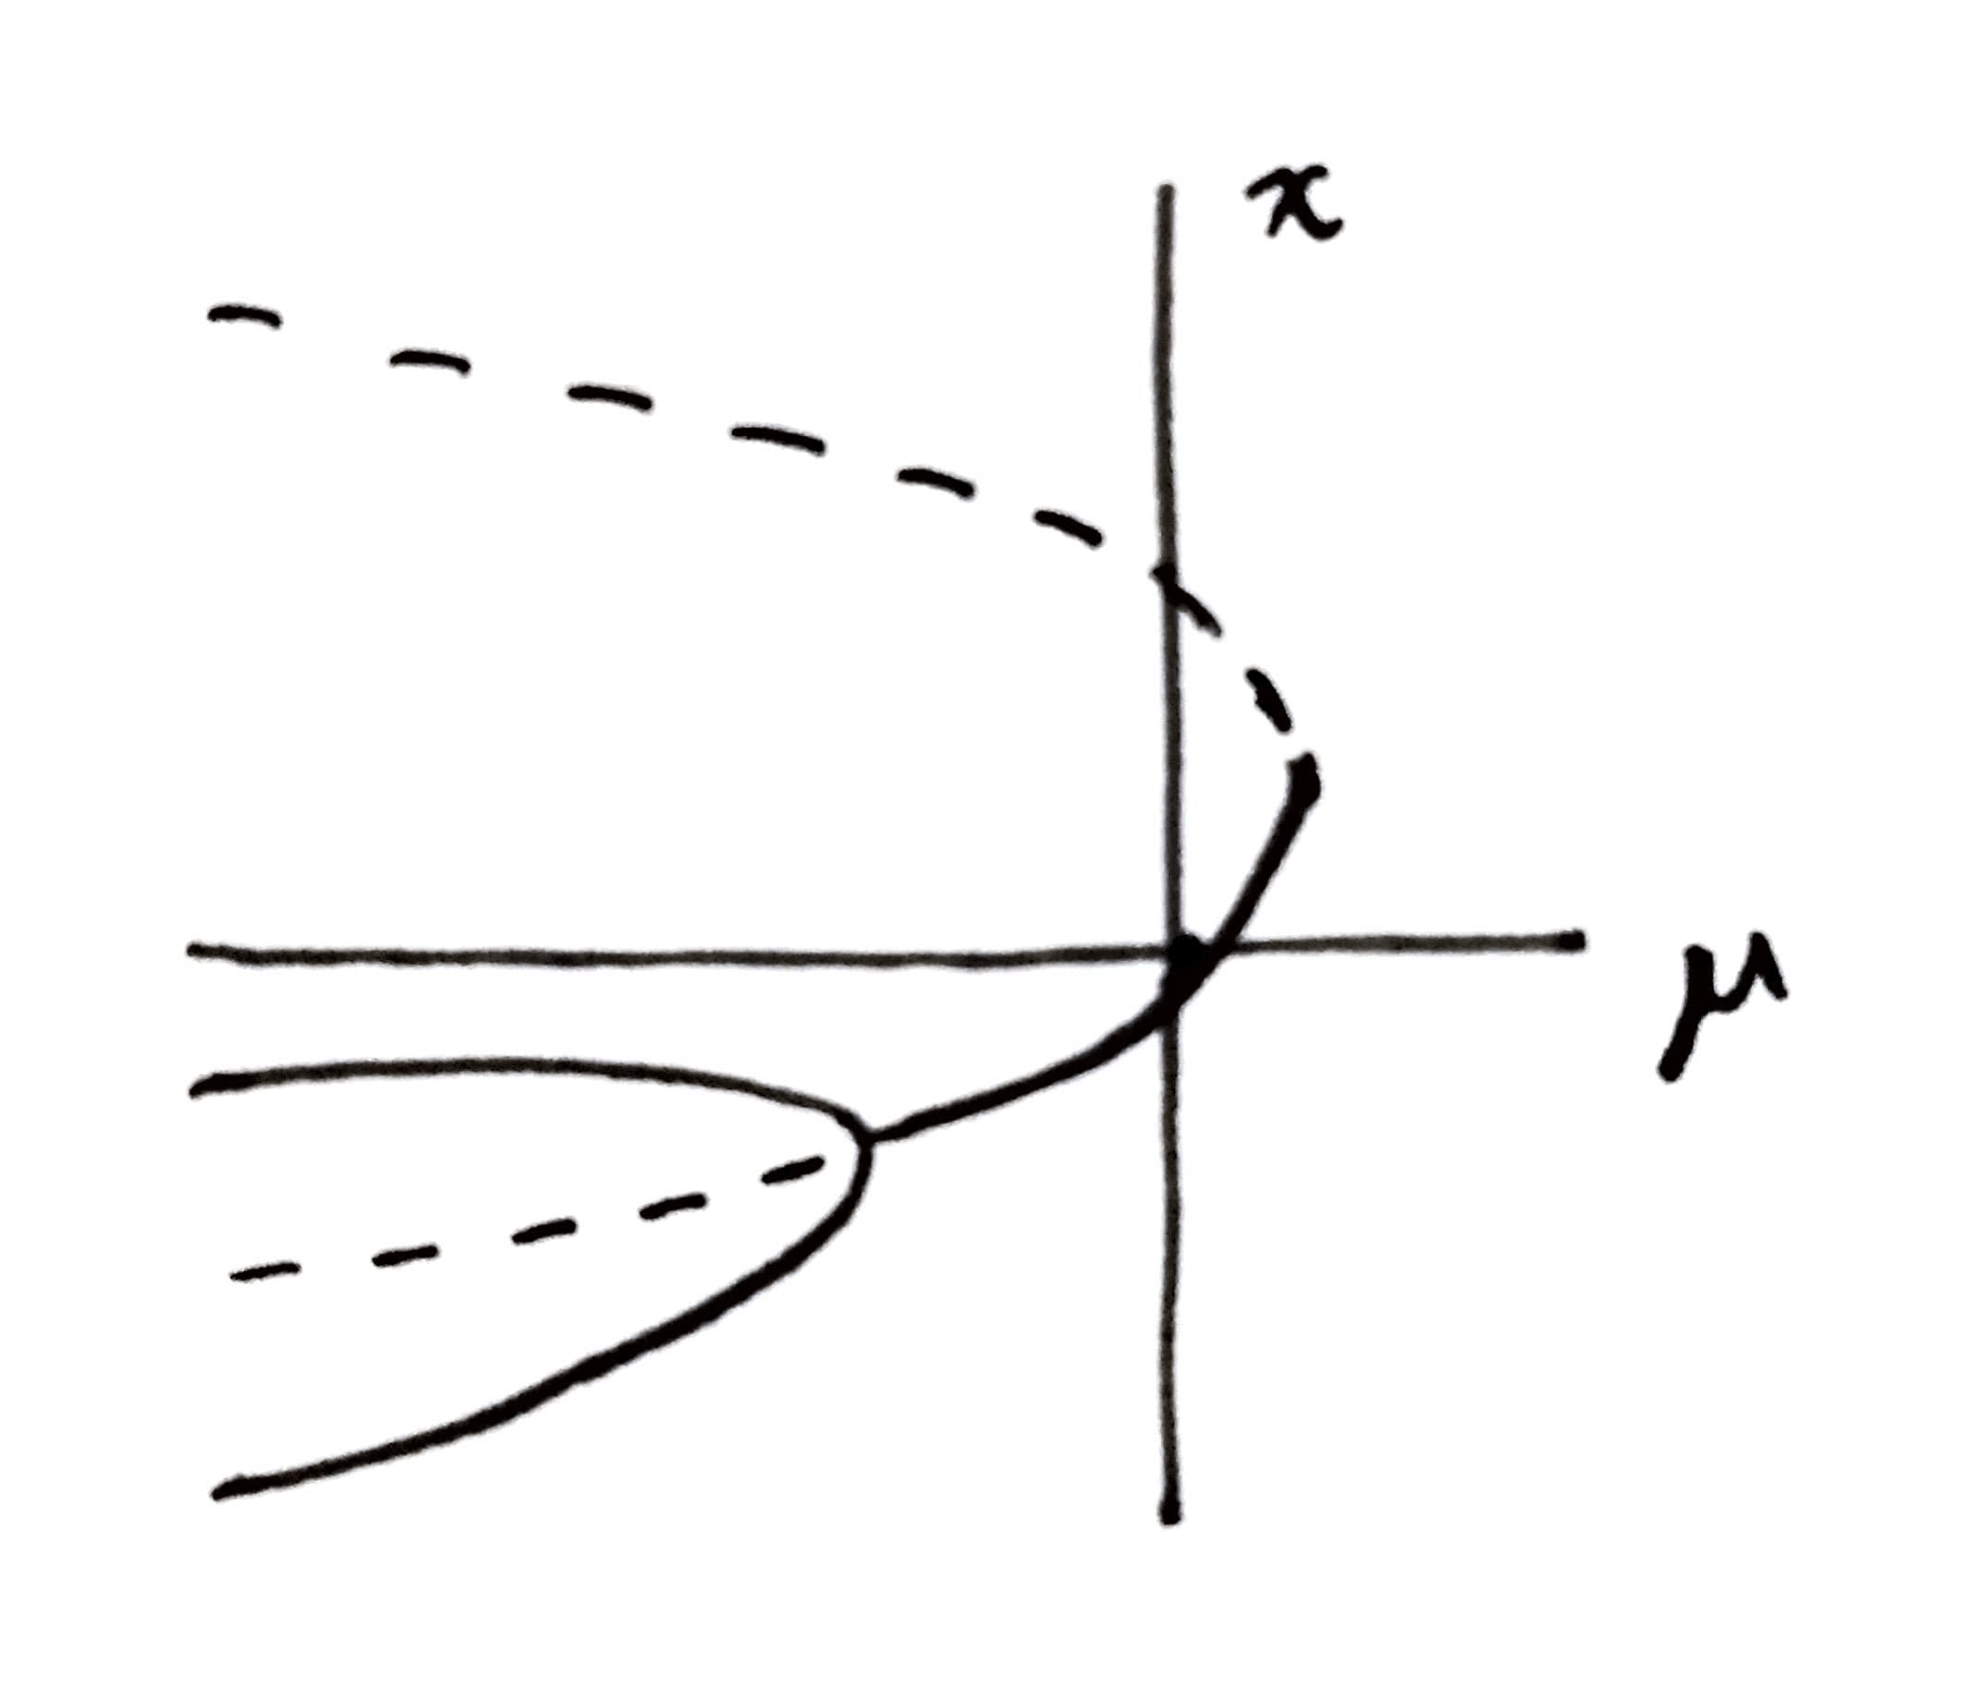
\includegraphics[height=0.3\textwidth]{img/2019F2.png}
        \end{center}
        
        \item A period-doubling bifurcation occurs when $f'(\widetilde x_-)$ passes through $-1$, which occurs at $\mu = -3/4$. Then, a saddle-node bifurcation occurs at $\mu = 1/4$.
        
    \end{enumerate}
    
\item
\begin{qbox}
Let
\[
\mathcal{E}[y(x)] = \int_0^1 \left[\frac{dy}{dx}\right]^2\,dx.
\]
Find the functions $y(x)$ for which $\mathcal{E}$ is extremal, subject to the constraints
\[
\int_0^1 [y(x)]^2\,dx = 1
\]
and
\[
y(0) = 0, \qquad y'(1) = 0
\]
where $y' = dy/dx$.
\end{qbox}

We let $h = y'^2 + \lambda y^2$ for some $\lambda \in \R$. Then, the Euler-Lagrange equation gives
\begin{align*}
\pp{h}{y} + \frac{d}{dx}\pp{h}{y'} 
&= 
0
\\
2\lambda y + \frac{d}{dx}\left(2y'\right) 
&=
0
\\
\lambda y + y'' &= 0
\end{align*}
We show that $\lambda \geq 0:$
\begin{align*}
    y'' &= -\lambda y \\
    \int y'' y &= -\lambda \int y^2 \\
    yy'\big\vert_0^1 - \int y'^2 &= -\lambda \int y^2
    &\textrm{(IBP)} \\
    - \int y'^2 &= -\lambda \int y^2 &\textrm{(Boundary Conds)}
\end{align*}
So, we have $\lambda = \mu^2$, and so our equation is
\[
y'' = -\mu^2 y.
\]
Solutions to this equation are 
\[
y = A\sin(\mu x) + B\cos(\mu x).
\]
The boundary condition $y(0) = 0$ yields $B = 0$, while the boundary condition $y'(1) = 0$ yields  
\[
\cos(\mu) = 0 \so \mu = k \pi + \frac{\pi}{2}, \quad k \in \Z.
\]
Now, we plug back in our equation into our integral constraint:
\begin{align*}
    1 &=
    \int_0^1 y^2\,dx 
    \\
    &=
    A^2\int_0^1 \cos^2\left[\left(k \pi + \frac{\pi}{2}\right)x\right]\,dx \\
    &= 
    \frac{A^2}{2}\int_0^1\left(1 + \cos\left[\left(2k \pi + \pi\right)x\right]\right)\,dx
    \\
    &= 
    \frac{A^2}{2}\int_0^1\left(1 + \cos\left(\pi x\right)\right)\,dx 
    \\
    &=
    \frac{A^2}{2}\left[1 + \pi\sin(\pi x)\big\vert_0^1\right] \\
    &=
    \frac{A^2}{2}
\end{align*}
So, we get $A^2 = 2$, and so $A = \pm \sqrt 2$. So, our final solution is
\[
y(x) = \pm\sqrt{2}\sin\left(\left(k\pi + \frac{\pi}{2}\right)x\right),\quad k \in \Z.
\]

% Solutions to the above ODE are given by
% \[
% y(x) = Ae^{\sqrt{-\lambda}x} + Be^{-\sqrt{-\lambda} x},
% \]
% for some constants $A, B$. We plug in our initial conditions, starting with $y(0) = 0$.
% \begin{align*}
%     y(0) = A + B &= 0 \qquad \rightarrow \qquad y(x) = A\left(e^{\sqrt{-\lambda}x} - e^{-\sqrt{-\lambda}x}\right)
% \end{align*}
% Now, we plug in $y'(1) = 0$.
% \begin{align*}
%     y'(x) &= A\sqrt{-\lambda}\left(e^{\sqrt{-\lambda}x} + e^{-\sqrt{-\lambda}x}\right)
%     \\
%     0 &= A\sqrt{-\lambda}\left(e^{\sqrt{-\lambda}} + e^{-\sqrt{-\lambda}}\right)
% \end{align*}
% This equation tells us that $\lambda$ must be positive. If it were negative, then all of the factors on the righthand side would be positive, and so we would have to have $A = 0$, which would only be the trivial solution. So, we have $\lambda = \mu^2$. Now, the equation becomes
% \begin{align*}
%     0 &= A\mu \left(e^{i\mu} + e^{-i\mu}\right)
%     \\
%     e^{i\mu} &= -e^{-i\mu}
%     \\
%     e^{i2\mu} &= -1
%     \\
%     \mu &= \frac{\pi}{2} + n\pi, \qquad n \in \Z
% \end{align*}
% So, we now have
% \[
% y(x) = A\left(e^{i(n\pi + \pi/2)x} - e^{-i(n\pi + \pi/2) x}\right).
% \]
% Finally, we plug this into our integral constraint to solve for $A$.
% \begin{align*}
%     1 &= \int_0^1\left(A\left(e^{i(n\pi + \pi/2)x} - e^{-i(n\pi + \pi/2) x}\right)\right)^2\,dx 
%     \\
%     1 &= A^2\int_0^1\left(e^{i(2\pi n + \pi)x} - 2 + e^{-i(2\pi n + \pi) x}\right)\,dx 
%     \\
%     1 &= A^2\left(\frac{e^{i(2\pi n + \pi)x} - e^{-i(2\pi n + \pi) x}}{i(2\pi n + \pi)} - 2x \right)\bigg\vert_0^1
%     \\
%     1 &= A^2\left(\frac{-1 + 1 - 1 + 1}{i(2\pi n + \pi)} - 2 \right)
%     \\
%     A^2 &= -\frac{1}{2}
%     \\
%     A &= \pm \frac{i}{\sqrt 2}
% \end{align*}
% So, the resulting functions for which $\mathcal E$ is extremal are
% \begin{align*}
% y(x) &= \pm \frac{i}{\sqrt 2}\left(e^{i \mu x} - e^{-i \mu x}\right)
% \\
% &= \pm \sqrt{2}\sin(\mu x)
% \\
% &= \pm \sqrt{2}\sin\left(\left(\frac{\pi}{2} + n\pi\right) x\right), \qquad n \in \N.
% \end{align*}

\item
\begin{qbox}
Let $\mathcal D$ be the disk of radius $a$ in $\R^2$, i.e. $x^2 + y^2 \leq a^2$. Let $h(x, y)$ be a single valued function of $x$ and $y$ which describes a surface above $\mathcal D$ which is fixed on the boundary to 
\[h(a \cos(\theta), a \sin(\theta)) = f(\theta).\]
\begin{itemize}
    \item[\textbf{(a)}] Find the functional $\mathcal S[h(x, y)]$ which computes the surface area of $h(x, y)$.
    \item[\textbf{(b)}] Determine the equation for the function $h(x, y)$ which minimizes $\mathcal S[h(x, y)]$.
    \item[\textbf{(c)}] Linearize the equation in \textbf{(b)} and solve it subject to the boundary condition
    \[ h(a \cos(\theta), a \sin(\theta)) = \cos^2(\theta).\]
\end{itemize}
\end{qbox}

\begin{enumerate}
    \item $\displaystyle{\mathcal S[h(x,y)] = \iint_{\mathcal D} \sqrt{h_x^2 + h_y^2 + 1}\,dx\,dy}$
    
    \item We label the integrand of $\mathcal S$ by $f$. Then, the Euler-Lagrange equation for this problem is
    \[
    \pp{f}{h} - \frac{\partial}{\partial x} \pp{f}{h_x} - \frac{\partial}{\partial y} \pp{f}{h_y} = 0.
    \]
    Since $\partial f/\partial h = 0$, this becomes
    \begin{align*}
        \frac{\partial}{\partial x} \left(\frac{h_x}{\sqrt{h_x^2 + h_y^2 + 1}}\right) +  \frac{\partial}{\partial y} \left(\frac{h_y}{\sqrt{h_x^2 + h_y^2 + 1}}\right)
        &= 0
        \\
        \frac{h_{xx} \sqrt{\cdot} - 2h_x(h_xh_{xx} + h_yh_{xy})/\sqrt{\cdot} }{h_x^2 + h_y^2 + 1} 
        + 
        \frac{h_{yy} \sqrt{\cdot} - 2h_y(h_yh_{yy} + h_xh_{xy})/\sqrt{\cdot} }{h_x^2 + h_y^2 + 1}
        &= 0
        \\
        h_{xx} (h_x^2 + h_y^2 + 1) - 2h_x(h_xh_{xx} + h_yh_{xy})
        + 
        h_{yy} (h_x^2 + h_y^2 + 1) - 2h_y(h_yh_{yy} + h_xh_{xy})
        &= 0
        \\
        h_{xx} - h_x^2h_{xx} + h_y^2h_{xx} - 4h_xh_yh_{xy}
        + 
        h_x^2h_{yy} - h_y^2h_{yy} + h_{yy}
        &= 0
    \end{align*}
    \item Linearizing the equation in \textbf{(b)} yields
    \[
    h_{xx} + h_{yy} = 0 \qquad \rightarrow \qquad \nabla^2 h = 0 \quad \textrm{(Laplace's Equation)}
    \]
    Solutions to Laplace's Equation on the interior of the disk have the form
    \[
    h(r,\theta) = \frac{\alpha_0}{2} + \sum_{n=1}^\infty r^n \left(\alpha_n \cos(n\theta) + \beta_n \sin(n\theta)\right).
    \]
    Since $h(a, \theta) = \cos^2(\theta)$, our goal is to find the coefficients $\alpha_0, \alpha_n, \beta_n$ such that
    \[
    \cos^2\theta = \frac{\alpha_0}{2} + \sum_{n=1}^\infty a^n \left(\alpha_n \cos(n\theta) + \beta_n \sin(n\theta)\right).
    \]
    Notice that $\cos^2\theta = 1/2 + 1/2\cdot \cos(2\theta)$. Written in this format, our coefficients are obvious: $\alpha_0 = 1$, $\alpha_2 = 1/2a^2$, and all other coefficients are zero.
    % We calculate the coefficients:
    % \begin{align*}
    %     \alpha_0 &= \frac{1}{\pi}\int_{-\pi}^\pi \cos^2\theta\,d\theta = \frac{1}{\pi}\cdot \pi = 1 \\
    %     \alpha_n &= \frac{1}{a^n\pi}\int_{-\pi}^\pi \cos(n\theta)\cos^2(\theta)\,d\theta
    %     \\
    %     &= \frac{1}{a^n\pi}\int_{-\pi}^\pi \cos(n\theta)\left(\frac{1}{2}\cos(2\theta) + \frac{1}{2}\right)\,d\theta
    %     \\
    %     &= \frac{1}{2a^n\pi}\int_{-\pi}^\pi \cos(n\theta)\cos(2\theta)\,d\theta + \frac{1}{2a^n\pi}\int_{-\pi}^\pi \cos(n\theta)\,d\theta
    %     \\
    %     &= \frac{1}{4a^n\pi}\left(\int_{-\pi}^\pi \cos((n-2)\theta)\,d\theta + \int_{-\pi}^\pi\cos((n+2)\theta)\,d\theta\right) + 0
    %     \\
    %     &=
    %     \frac{1}{4a^n\pi}\left(\frac{\sin((n-2)\theta)}{n-2} + \frac{\sin((n+2)\theta)}{n+2}\right)\bigg\vert_{-\pi}^\pi &(n \ne 2)
    %     \\
    %     &= 0 &(n \ne 2)
    %     \\
    %     \alpha_2 &=
    %     \frac{1}{4a^2\pi}\left(\int_{-\pi}^\pi \cos(0)\,d\theta + \int_{-\pi}^\pi\cos(4\theta)\,d\theta\right)
    %     \\
    %     &=
    %     \frac{1}{4a^2\pi}\left(2\pi+ \frac{\sin(4\theta)}{4}\bigg\vert_{-\pi}^\pi\right)
    %     \\
    %     &=
    %     \frac{1}{2a^2}
    %     \\
    %     \beta_n &= \frac{1}{a^n\pi}\int_{-\pi}^\pi \sin(n\theta)\cos^2(\theta)\,d\theta\\
    %     &= 0 &\textrm{(Odd func over symmetric interval)}
    % \end{align*}
    So, we end up with
    \[
    h(r,\theta) = \frac{1}{2} + \frac{r^2}{2a^2}\cos(2\theta).
    \]
\end{enumerate}

\item 
\begin{qbox}
Use the WKB method to find an approximate solution to the following problem:
\[
\epsilon y'' + 2y' + 2y = 0,
\]
with $y(0) = 0$ and $y(1) = 1$.
\end{qbox}

The WKB expansion for $y$ and its associated derivatives is (assuming $\alpha > 0$):
\begin{align*}
    y &\thicksim e^{\theta(x)/\epsilon^\alpha}\left(y_0 + \epsilon^\alpha y_1 \right) \\
    y' &\thicksim e^{\theta(x)/\epsilon^\alpha}\left(\epsilon^{-\alpha}\theta_x y_0 + y_0' + \theta_xy_1 + \cdots\right) \\
    y'' &\thicksim e^{\theta(x)/\epsilon^\alpha}\left(\epsilon^{-2\alpha}\theta_x^2 y_0 + \epsilon^{-\alpha}\left(\theta_{xx} y_0 + 2\theta_x y_0' + \theta_x^2 y_1\right) + \cdots\right)
\end{align*}
Plugging this into our equation and canceling the exponential terms yields
\begin{align*}
    \epsilon\left(\epsilon^{-2\alpha}\theta_x^2 y_0 + \epsilon^{-\alpha}\left(\theta_{xx} y_0 + 2\theta_x y_0' + \theta_x^2 y_1\right) \right) + 2\left(\epsilon^{-\alpha}\theta_x y_0 + y_0' + \theta_xy_1 \right) + 2 \left(y_0 + \epsilon^\alpha y_1 \right) &= 0
    \\
    \undernum{\epsilon^{-2\alpha + 1}\theta_x^2 y_0}{1} + \undernum{\epsilon^{-\alpha + 1}\left(\theta_{xx} y_0 + 2\theta_x y_0' + \theta_x^2 y_1\right)}{2} + \undernum{\epsilon^{-\alpha}2\theta_x y_0}{3} + \undernum{2y_0' + 2\theta_xy_1 + 2y_0}{4} + \undernum{\epsilon^\alpha 2 y_1}{5} &= 0
\end{align*}
As we assume $\alpha > 0$, we need only match terms $\circled{1}$, $\circled{3}$, and $\circled{4}$ for leading order.
\begin{alignat*}{3}
    \circled{1}\thicksim \circled{3} : &\ -2\alpha + 1 &= -\alpha &\so \alpha = 1 &\so \circled{1}\  \circled{3}: \mathcal{O}(1/\epsilon), \quad \circled{4}: \mathcal{O}(1)\quad  \checkmark
\end{alignat*}
Since $\alpha = 1$ works, we don't need to check the rest. We examine our leading-order equation, $\mathcal{O}(1/\epsilon)$:
\begin{align*}
    \theta_x^2 y_0 + 2\theta_x y_0 &= 0 \\
    \theta_x(\theta_x + 2)y_0 &= 0
    \\
    \theta_x(\theta_x + 2) &= 0
    \\
    \theta_x &= 0, -2
\end{align*}
So, our two options for $\theta(x)$ are
\[
\theta(x) = 0 \qquad \textrm{and} \qquad \theta(x) = -2x.
\]
Now, we examine our equation of next-leading order, $\mathcal{O}(1):$
\begin{align*}
    \theta_{xx} y_0 + 2\theta_x y_0' + \theta_x^2 y_1 + 2y_0' + 2\theta_xy_1 + 2y_0 &= 0
    \\
    \theta_{xx} y_0 + 2\theta_x y_0' + 2y_0' + 2y_0 + \theta_x(\theta_x + 2) y_1 &= 0
    \\
    \theta_{xx} y_0 + 2\theta_x y_0' + 2y_0' + 2y_0 &= 0
\end{align*}
First, we consider the case $\theta(x) = 0$. With this $\theta$, our equation becomes
\begin{align*}
    2y_0' + 2y_0 &= 0 \\
    y_0' &= -y_0 \\
    y_0 &= Ae^{-x}
\end{align*}
Next, we consider the case $\theta(x) = -2x$. With this $\theta$, our equation becomes
\begin{align*}
    -4 y_0' + 2y_0' + 2y_0 &= 0 \\
    y_0' &= y_0 \\
    y_0 &= Be^x
\end{align*}
Putting these together, we get the approximation
\[
y \thicksim Ae^{-x} + Be^{-2x/\epsilon + x}.
\]
Now, we plug in our boundary conditions to solve for $A, B$.
\begin{align*}
    y(0) = 0 \so 0 &= A + B \so y \thicksim A\left(e^{-x} - e^{-2x/\epsilon + x}\right) \\
    y(1) = 1 \so 1 &= A\left(e^{-1} - e^{1 - 2/\epsilon}\right)
\end{align*}
So, in the end, our final approximation is
\[
y \thicksim \frac{e^{-x} - e^{-2x/\epsilon + x}}{e^{-1} - e^{1 - 2/\epsilon}}
\]

\item 
\begin{qbox}
Consider the motion of a damped pendulum. The evolution of the position of the end of the pendulum $y(t)$ is
described by
\[
\epsilon \frac{d^2 y}{dt^2} + \frac{dy}{dt} + \sin(y(t)) = 0, \qquad \qquad y(0) = \epsilon, \quad y'(0) = 0,
\]
where $\epsilon \ll 1$. Use the method of multiple scales to find an approximate solution to the IVP above.
\end{qbox}

We begin by rescaling, setting $y = \epsilon x$ so that our boundary conditions are of order 1:
\[
\epsilon^3 \ddot x + \epsilon \dot x + \sin(\epsilon x) = 0, \qquad x(0) = 1, x'(0) = 0
\]
Expanding $\sin(\epsilon x)$ about $x = 0$, we get
\begin{align*}
    \epsilon^3 \ddot x + \epsilon \dot x + \epsilon x - \frac{1}{6}\epsilon^3 x^3 + \cdots &= 0 \\
    \epsilon^2 \ddot x + \dot x + x - \frac{1}{6}\epsilon^2 x^3 + \cdots &= 0
\end{align*}
Now, we let $t_1 = t$ and $t_2 = \epsilon^\alpha t$, where $\alpha \ne 0$. Then, our equation becomes
\begin{align*}
    \epsilon^2\left(\partial^2_{t_1} + 2\epsilon^\alpha \partial_{t_1}\partial_{t_2} + \epsilon^{2\alpha} \partial_{t_2}^2\right)x + \left(\partial_{t_1} + \epsilon^{\alpha} \partial_{t_2}\right)x + x - \frac{1}{6}\epsilon^2 x^3 &= 0
    \\
    \big(\epsilon^2\partial^2_{t_1} + 2\epsilon^{\alpha + 2} \partial_{t_1}\partial_{t_2} + \undernum{\epsilon^{2 + 2\alpha} \partial_{t_2}^2}{1}\big)x + \big(\undernum{\partial_{t_1}}{2} + \undernum{\epsilon^{\alpha} \partial_{t_2}}{3}\big)x + x - \frac{1}{6}\epsilon^2 x^3 &= 0
\end{align*}
Matching for leading order, if we try $\circled 1 \thicksim \circled 3$, we get $2 + 2\alpha = \alpha$, which yields $\alpha = -2$. This would indeed make these terms leading order, so we go with it. Our equation becomes
\[
\big(\epsilon^2\partial^2_{t_1} + 2\partial_{t_1t_2} + \epsilon^{-2} \partial_{t_2}^2\big)x + \big(\partial_{t_1} + \epsilon^{-2} \partial_{t_2}\big)x + x - \frac{1}{6}\epsilon^2 x^3 = 0
\]
Our leading order equation is $\Ord{\epsilon^{-2}}:$
\begin{align*}
\partial_{t_2}^2 x + \partial_{t_2} x &= 0 \so
\partial_{t_2} x_0 = A(t_1)e^{-t_2} \so x_0 = A(t_1)e^{-t_2} + B(t_1)
\end{align*}
The boundary condition $x(0) = 1$ yields $A(0) + B(0) = 1$. Our other boundary condition is
\begin{align*}
(\partial_{t_1} + \epsilon^{-2}\partial_{t_2} )x\big\vert_{0,0} = 0
\so
A(0) = 0
\end{align*}
So, our boundary conditions are $A(0) = 0$ and $B(0) = 1$. Next, we add a term to our approximation: $x = x_0 + \epsilon^2 x_1$. Our equation is now
\[
\big(\epsilon^2\partial^2_{t_1} + 2\partial_{t_1t_2} + \epsilon^{-2} \partial_{t_2}^2\big)(x_0 + \epsilon^2 x_1) + \big(\partial_{t_1} + \epsilon^{-2} \partial_{t_2}\big)(x_0 + \epsilon^2 x_1) + x_0 + \epsilon^2 x_1 - \frac{1}{6}\epsilon^2 (x_0 + \epsilon^2 x_1)^3 = 0
\]
Our next-leading order equation is $\Ord{1}:$
\begin{align*}
2\partial_{t_1t_2}x_0 + \partial_{t_2}^2x_1 + \partial_{t_1}x_0 + \partial_{t_2}x_1 + x_0 
&= 0
\\
\left(\partial_{t_2}^2x_1 + \partial_{t_2}x_1 \right) + 2\partial_{t_1t_2}x_0 +  \partial_{t_1}x_0 + x_0 &= 0
% \\
% \left(\partial_{t_2}^2x_1 + \partial_{t_2}x_1 \right) + 2\left(-A'(t_1)\sin(t_2) + B'(t_1)\cos(t_2)\right) +  A'(t_1)\cos(t_2) + B'(t_1)\sin(t_2) + A(t_1)\cos(t_2) + B(t_1)\sin(t_2)
% &=
% 0
\end{align*}
Our partial derivatives of $x_0$ are
\begin{align*}
    \partial_{t_1}x_0
    &=
    A'(t_1)e^{-t_2} + B'(t_1)
    \\
    \partial_{t_1t_2}x_0
    &=
    -A'(t_1)e^{-t_2}
\end{align*}
So, our equation is
\begin{align*}
    \left(\partial_{t_2}^2x_1 + \partial_{t_2}x_1 \right)
    -2A'(t_1)e^{-t_2} + A'(t_1)e^{-t_2} + B'(t_1) + A(t_1)e^{-t_2} + B(t_1)
    &=
    0
\end{align*}
So, in order to eliminate secular terms, we require
\begin{alignat*}{3}
    -A'(t_1)+A(t_1) &= 0 
    \andso 
    A &= c_1e^{t_1}
    \\
    B'(t_1) +B(t_1) &= 0
    \andso
    B &= c_2e^{-t_1}
\end{alignat*}
The boundary conditions $A(0) = 0$ and $B(0) = 1$ yield $c_1 = 0$ and $c_2 = 1$. So, we have $A = 0$, $B = e^{-t_1}$. In total, our final solution is therefore
\begin{align*}
    x &\thicksim e^{-t} \so y \thicksim \epsilon e^{-t}.
\end{align*}






% We let $t_1 = t$ and $t_2 = \epsilon^\alpha t$, where $\alpha \ne 0$. Since $y(0) = \epsilon$, we approximate $y$ by $y \thicksim \epsilon y_0 + \epsilon^\beta y_1$, where $\beta > 1$. With this assumption, we can now write $\sin(\epsilon y_0 + \epsilon^\beta y_1) \thicksim \epsilon y_0 + \epsilon^\beta y_1$. So, our equation becomes
% \[
% \epsilon\left(\partial^2_{t_1} + 2\epsilon^\alpha \partial_{t_1}\partial_{t_2} + \epsilon^{2\alpha} \partial_{t_2}^2\right)(\epsilon y_0 + \epsilon^\beta y_1) + \left(\partial_{t_1} + \epsilon^\alpha \partial_{t_2}\right)(\epsilon y_0 + \epsilon^\beta y_1) + \epsilon y_0 + \epsilon^\beta y_1 = 0,
% \]
% with boundary conditions
% \begin{align*}
% (\epsilon y_0 + \epsilon^\beta y_1)\big\vert_{t_1 = t_2 = 0} &= \epsilon
% \\
% (\partial_{t_1} + \epsilon^\alpha \partial_{t_2})(\epsilon y_0 + \epsilon^\beta y_1)\big\vert_{t_1 = t_2 = 0} &= 0.
% \end{align*}
% First, we can factor an $\epsilon$ out of our equation, which simplifies it to:
% \[
% \left(\epsilon\partial^2_{t_1} + 2\epsilon^{\alpha+1} \partial_{t_1}\partial_{t_2} + \epsilon^{2\alpha + 1} \partial_{t_2}^2\right)(y_0 + \epsilon^{\beta - 1} y_1) + \left(\partial_{t_1} + \epsilon^\alpha \partial_{t_2}\right)(y_0 + \epsilon^{\beta - 1} y_1) + y_0 + \epsilon^{\beta - 1} y_1 = 0.
% \]
% To match our expressions, we temporarily neglect the $\epsilon^{\beta - 1} y_1$ terms, since they will never be of leading order: 
% \[
% \undernum{\epsilon\partial^2_{t_1}y_0}{1} + \undernum{\epsilon^{\alpha+1}2 \partial_{t_1}\partial_{t_2}y_0}{2} + \undernum{\epsilon^{2\alpha + 1} \partial_{t_2}^2y_0}{3} + \undernum{\partial_{t_1}y_0 + y_0}{4} + \undernum{\epsilon^\alpha \partial_{t_2}y_0}{5} = 0
% \]
% Now, we match terms.
% \begin{alignat*}{5}
%     \circled{1} &\thicksim \circled{2}: &\  1 &= \alpha + 1 &\so \alpha &= 0 &\qquad (\times)
%     \\
%     \circled{1} &\thicksim \circled{3}: &\  1 &= 2\alpha + 1 &\so \alpha &= 0 &\qquad (\times)
%     \\
%     \circled{1} &\thicksim \circled{5}: &\  1 &= \alpha &\so \alpha &= 1 &\qquad \rightarrow &\qquad \circled{1}\ \circled{5}: \mathcal{O}(\epsilon), \quad \circled{4}: \mathcal{O}(1) \quad (\times)
%     \\
%     \circled{2} &\thicksim \circled{3}: &\  \alpha + 1 &= 2\alpha + 1 &\so \alpha &= 0 &\qquad (\times)
%     \\
%     \circled{2} &\thicksim \circled{4}: &\  \alpha + 1 &= 0 &\so \alpha &= -1 &\qquad \rightarrow &\qquad \circled{2}\ \circled{4}: \mathcal{O}(1), \quad \circled{3}\ \circled{5}: \mathcal{O}(\epsilon^{-1}) \quad (\checkmark)
% \end{alignat*}
% So, we have $\alpha = -1$. Briefly, we rewrite our boundary conditions with this new information:
% \begin{align*}
%     \left(\epsilon y_0 + \epsilon^{\beta} y_1\right)\big\vert_{t_1 = t_2 = 0} &= \epsilon
%     \\
%     \left(\epsilon\partial_{t_1}y_0 + \partial_{t_2}y_0 + \epsilon^\beta \partial_{t_1}y_1 + \epsilon^{\beta - 1}\partial_{t_2}y_1\right)\big\vert_{t_1 = t_2 = 0} &= 0
% \end{align*}
% Now, we examine the leading order of our differential equation, $\mathcal{O}(1/\epsilon)$:
% \begin{align*}
%     \partial^2_{t_2}y_0 + \partial_{t_2} y_0 &= 0
%     \\
%     \partial_{t_2} w + w &= 0 &(w = \partial_{t_2} y_0)
%     \\
%     w &= c_1(t_1)e^{-t_2}
%     \\
%     \partial_{t_2} y_0 &= c_1(t_1)e^{-t_2}
%     \\
%     y_0 &= c_1(t_1)e^{-t_2} + c_2(t_1).
% \end{align*}
% Looking to our first boundary condition, the $\mathcal{O}(\epsilon)$ term gives $y_0(0, 0) = 1$, which therefore yields
% \[
% 1 = c_1(0) + c_2(0).
% \]
% Looking to our second boundary condition, the $\mathcal{O}(1)$ terms give $\partial_{t_2}y_0(0, 0) = 0$, which yields
% \begin{align*}
%     -c_1(t_1) e^{-t_2} &= 0
%     \\
%     c_1(0) &= 0 \so c_2(0) = 1.
% \end{align*}
% Now, to examine our next-greatest leading-order term in our equation, we must match for $\beta$ to get terms of order 1. As before, we neglect higher-order terms to match:
% \begin{align*}
% \left(\epsilon^{-1} \partial_{t_2}^2\right)\epsilon^{\beta - 1} y_1 + \left(\epsilon^{-1} \partial_{t_2}\right)\epsilon^{\beta - 1} y_1 + \epsilon^{\beta - 1} y_1 &= 0
% \\
% \epsilon^{\beta - 2} \partial_{t_2}^2y_1 + \epsilon^{\beta - 2} \partial_{t_2}y_1 + \epsilon^{\beta - 1} y_1 &= 0
% \end{align*}
% Since $\beta = 1$ contradicts our assumptions, $\beta = 2$ is the natural choice. So, we can now examine our order 1 equation:
% \begin{align*}
%     2 \partial_{t_1}\partial_{t_2}y_0 + \partial_{t_1}y_0 + y_0 + \partial_{t_2}^2y_1 + \partial_{t_2}y_1 &= 0
%     \\
%     2 \partial_{t_1}\partial_{t_2}y_0 + \partial_{t_1}y_0 + y_0 &= 0
%     \\
%     -2c_1'(t_1)e^{-t_2} + c_1'(t_1)e^{-t_2} + c_2'(t_1) + c_1(t_1)e^{-t_2} + c_2(t_1) &= 0
%     \\
%     \left(-c_1'(t_1) + c_1(t_1)\right)e^{-t_2} + c_2'(t_1) + c_2(t_1) &= 0
%     \\
%     \left(-c_1'(t) + c_1(t)\right)e^{-t/\epsilon} + c_2'(t) + c_2(t) &= 0
% \end{align*}
% So, examining first the $e^{-t/\epsilon}$ timescale, we have:
% \begin{align*}
%     -c_1'(t) + c_1(t) &= 0 \\
%     c_1(t) &= A e^t
%     \\
%     c_1(0) &= A = 0
%     \\
%     &\Downarrow \\
%     c_1 &= 0.
% \end{align*}
% Now, examining our other timescale, we have
% \begin{align*}
%     c_2'(t) + c_2(t) &= 0 \\
%     c_2(t) &= B e^{-t} \\
%     c_2(0) &= B = 1 \\
%     &\Downarrow \\
%     c_2(t) &= e^{-t}
% \end{align*}
% So, finally, we end up with $y_0 = e^{-t}$, and so our leading-order approximation is
% \[
% y \thicksim \epsilon e^{-t}.
% \]

\end{enumerate}

\chapter*{Spring 2019}
\chaptermark{Spring 2019}
\addcontentsline{toc}{chapter}{Spring 2019}

\begin{enumerate}
    \item 
    \begin{qbox}
    Consider a rigid, flat object, of mass $m$ and length $\ell$, attached to a torsional spring of stiffness $\kappa$ in the presence of wind of speed $v$ (see Fig. 1). The equations of motion are
    \[
    \frac{m\ell^2}{4}\frac{d^2\theta}{dt^2} = -\kappa\theta + vc\frac{\ell}{2}\sin(\theta),
    \]
    where $c$ is a drag constant so that $vc$ has units of force. Assume that all constants listed above are positive (but keep in mind that $\theta(t)$ may be negative).
    
    \begin{center}
        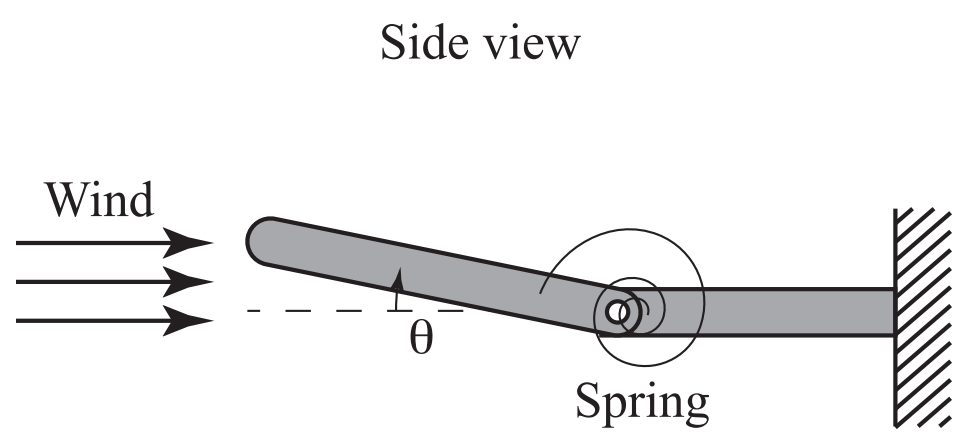
\includegraphics[width=0.45\textwidth]{img/2019S1.png}
    \end{center}
    
    \begin{itemize}
        \item[\textbf{(a)}] Use non-dimensionalization to show that the qualitative behavior of the system is defined by a single non-dimensional parameter.
        
        \item[\textbf{(b)}] Show that there is a conserved quantity.
        
        \item[\textbf{(c)}] As wind speed $v$ increases from 0, find a critical value of the non-dimensional parameter at which a bifurcation occurs, and identify the type of bifurcation.
        
        \item[\textbf{(d)}] Sketch the phase portrait at: \textbf{(i)} a wind speed just below the bifurcation, and \textbf{(ii)} a wind speed just after the bifurcation.
    \end{itemize}
    \end{qbox}
    
    \begin{enumerate}
        \item 
        First, we examine the dimensions of the parameters in our equation:
        \[
        [m] = M \qquad [\ell] = L \qquad [\kappa] = \frac{ML^2}{T^2} \qquad [v] = \frac{L}{T} \qquad [c] = \frac{M}{T}
        \]
        Since $\theta$ is unitless, we only need to work with $t$. We define the non-dimensional variable $\widetilde t$ and characteristic timescale $t_c$ so that $ t = t_c \widetilde t$. Then, our equation becomes
        \begin{align*}
            \frac{m\ell^2}{4}\frac{1}{t_c^2}\frac{d^2\theta}{d\widetilde t^2} 
            &= 
            -\kappa\theta + vc\frac{\ell}{2}\sin(\theta)
            \\
            \frac{d^2\theta}{d\widetilde t^2} 
            &= 
            -4\frac{\kappa}{m\ell^2}t_c^2\theta + 2\frac{vc\ell }{m\ell^2}t_c^2\sin(\theta)
            \\
            \frac{d^2\theta}{d\widetilde t^2} 
            &= 
            -4\frac{\kappa}{m\ell^2}t_c^2\theta + 2\frac{vc }{m\ell}t_c^2\sin(\theta)
        \end{align*}
        In the context of the problem, it seems more likely that we might encounter a windspeed of zero ($v = 0$) than a spring of zero stiffness ($\kappa = 0$), so we avoid using $v$ in our characteristic timescale. So, we set
        \[
        t_c^2 = \frac{m\ell^2}{2\kappa} 
        \qquad \qquad 
        \big(\textrm{verify dimensions: } \left[t_c\right] = \sqrt{\frac{ML^2}{ML^2/T^2}} = T\big)
        \]
        Now, our equation is
        \[
        \frac{d^2\theta}{d\widetilde t^2} = -2\theta + \frac{vc\ell}{\kappa}\sin\theta.
        \]
        We define the parameter $\mu = vc\ell/\kappa$ and verify that it is nondimensional:
        \[
        [\mu] = \frac{L/T \cdot M/T \cdot L}{ML^2/T^2} = 1
        \]
        So, our final, nondimensionalized equation is
        \[
        \ddot \theta = -2\theta + \mu \sin \theta.
        \]
        
        \item To show there's a conserved quantity, we go for the classic method of multiplying our equation by $\dot \theta$ on each side:
        \begin{align*}
            \ddot \theta \dot\theta
            &= 
            \left(-2\theta + \mu \sin \theta\right)\dot\theta
            \\
            \frac{d}{dt}\left(\frac{1}{2}\dot\theta^2\right)
            &=
            \frac{d}{dt}\left( -\theta^2 - \mu \cos\theta \right)
            \\
            \frac{1}{2}\dot\theta^2
            &=
            -\theta^2 - \mu \cos\theta + C
            \\
            \frac{1}{2}\dot\theta^2 + \theta^2 + \mu \cos\theta 
            &= 
            C.
        \end{align*}
        So, we have a conserved quantity $E(\theta, \dot \theta) = \dot\theta^2/2 + \theta^2 + \mu \cos\theta$.
        
        \item As $v$ increases from 0, so does $\mu$. We reduce our second-order ODE to a system of first-order ODEs:
        \begin{align*}
            \begin{cases}
            \:\dot \theta = \psi \\
            \dot \psi = -2\theta + \mu \sin\theta
            \end{cases}
        \end{align*}
        So, our equilibria occur when $\psi = 0$ and when $2\theta = \mu \sin\theta$. Comparing the graphs of $\theta$ and $(\mu/2)\cdot \sin\theta$, we see that we go from one fixed point to 3 fixed points when $\mu$ passes through 1:
        \begin{center}
        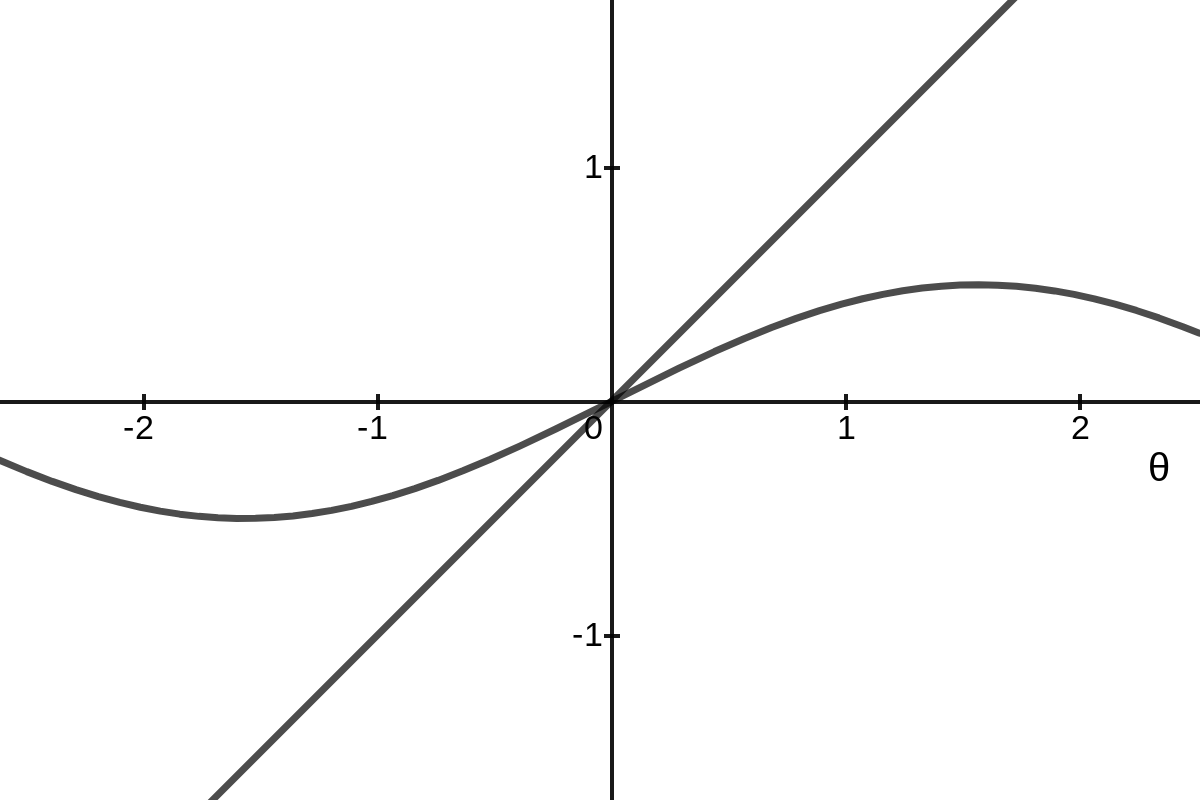
\includegraphics[width=0.3\textwidth]{img/2019S1-1.png}
        \quad 
        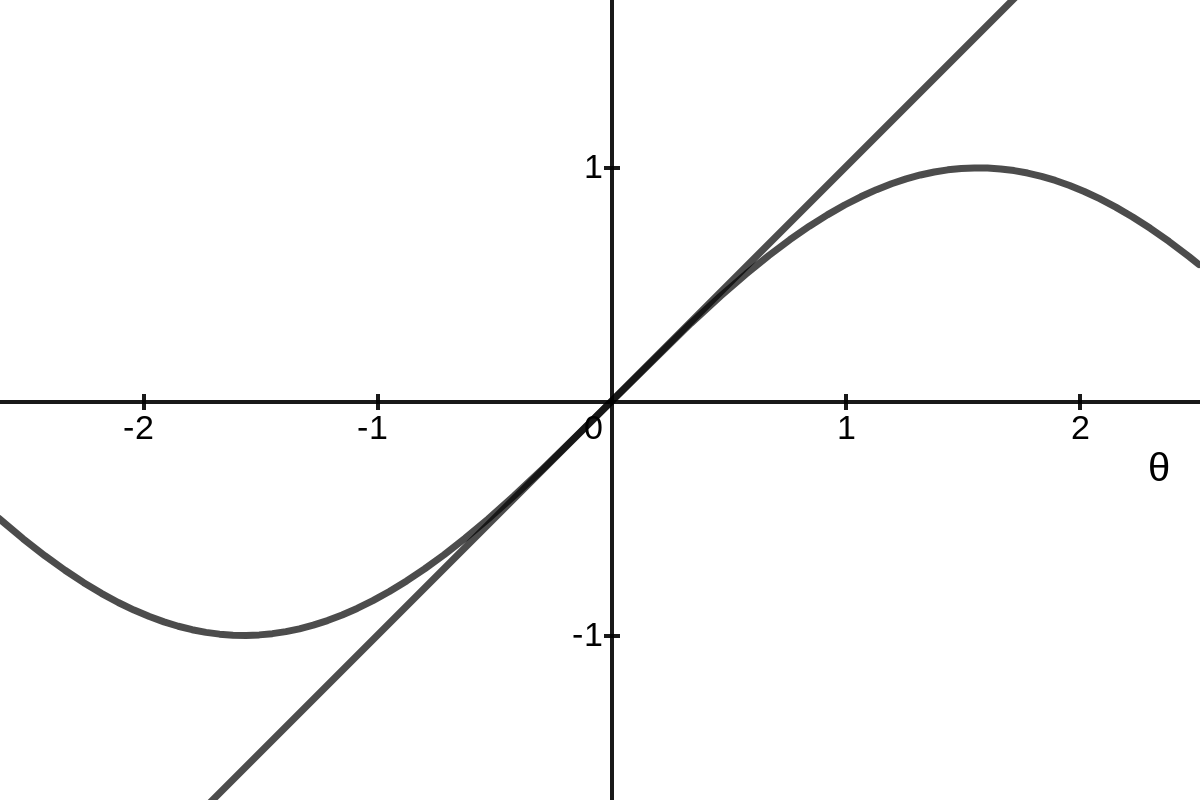
\includegraphics[width=0.3\textwidth]{img/2019S1-2.png}
        \quad 
        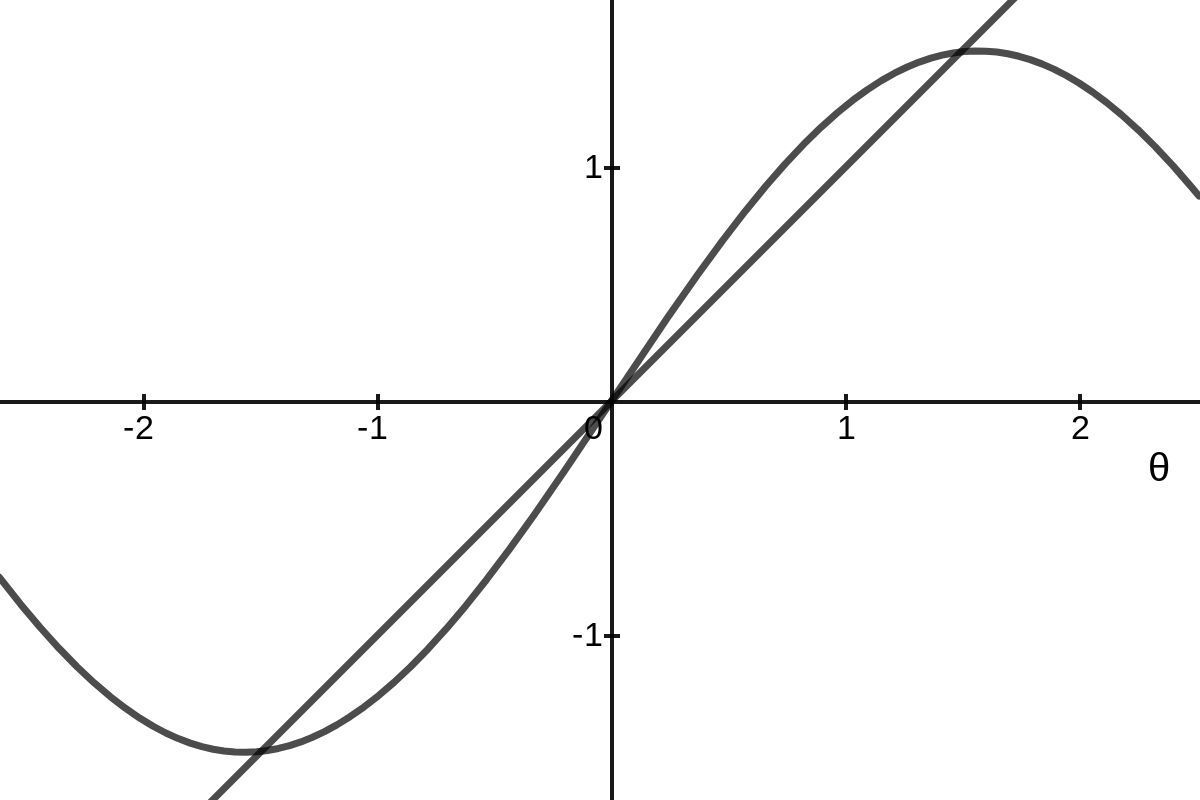
\includegraphics[width=0.3\textwidth]{img/2019S1-3.png}
        $\mu = \frac{1}{2}$ \qquad  \qquad\qquad \qquad \qquad \qquad \ \ $\mu = 1$ \qquad \qquad\qquad \qquad \qquad \qquad \ \  $\mu = \frac{3}{2}$
        \end{center}
        Since we go from 1 fixed point to 3 fixed points, and since the stability of our "inner" fixed point goes from stable to unstable as we add fixed points, we have a supercritical pitchfork bifurcation at $\mu = 1$.
        
        \item When $\mu$ is just below 1, we have a single stable fixed point at $(\theta, \psi) = (\theta, \dot\theta) = (0, 0)$. Since this is a conservative system, the only stable fixed points we have are centers, and so our phase portrait is a series of nested circles.
        
        \begin{center}
        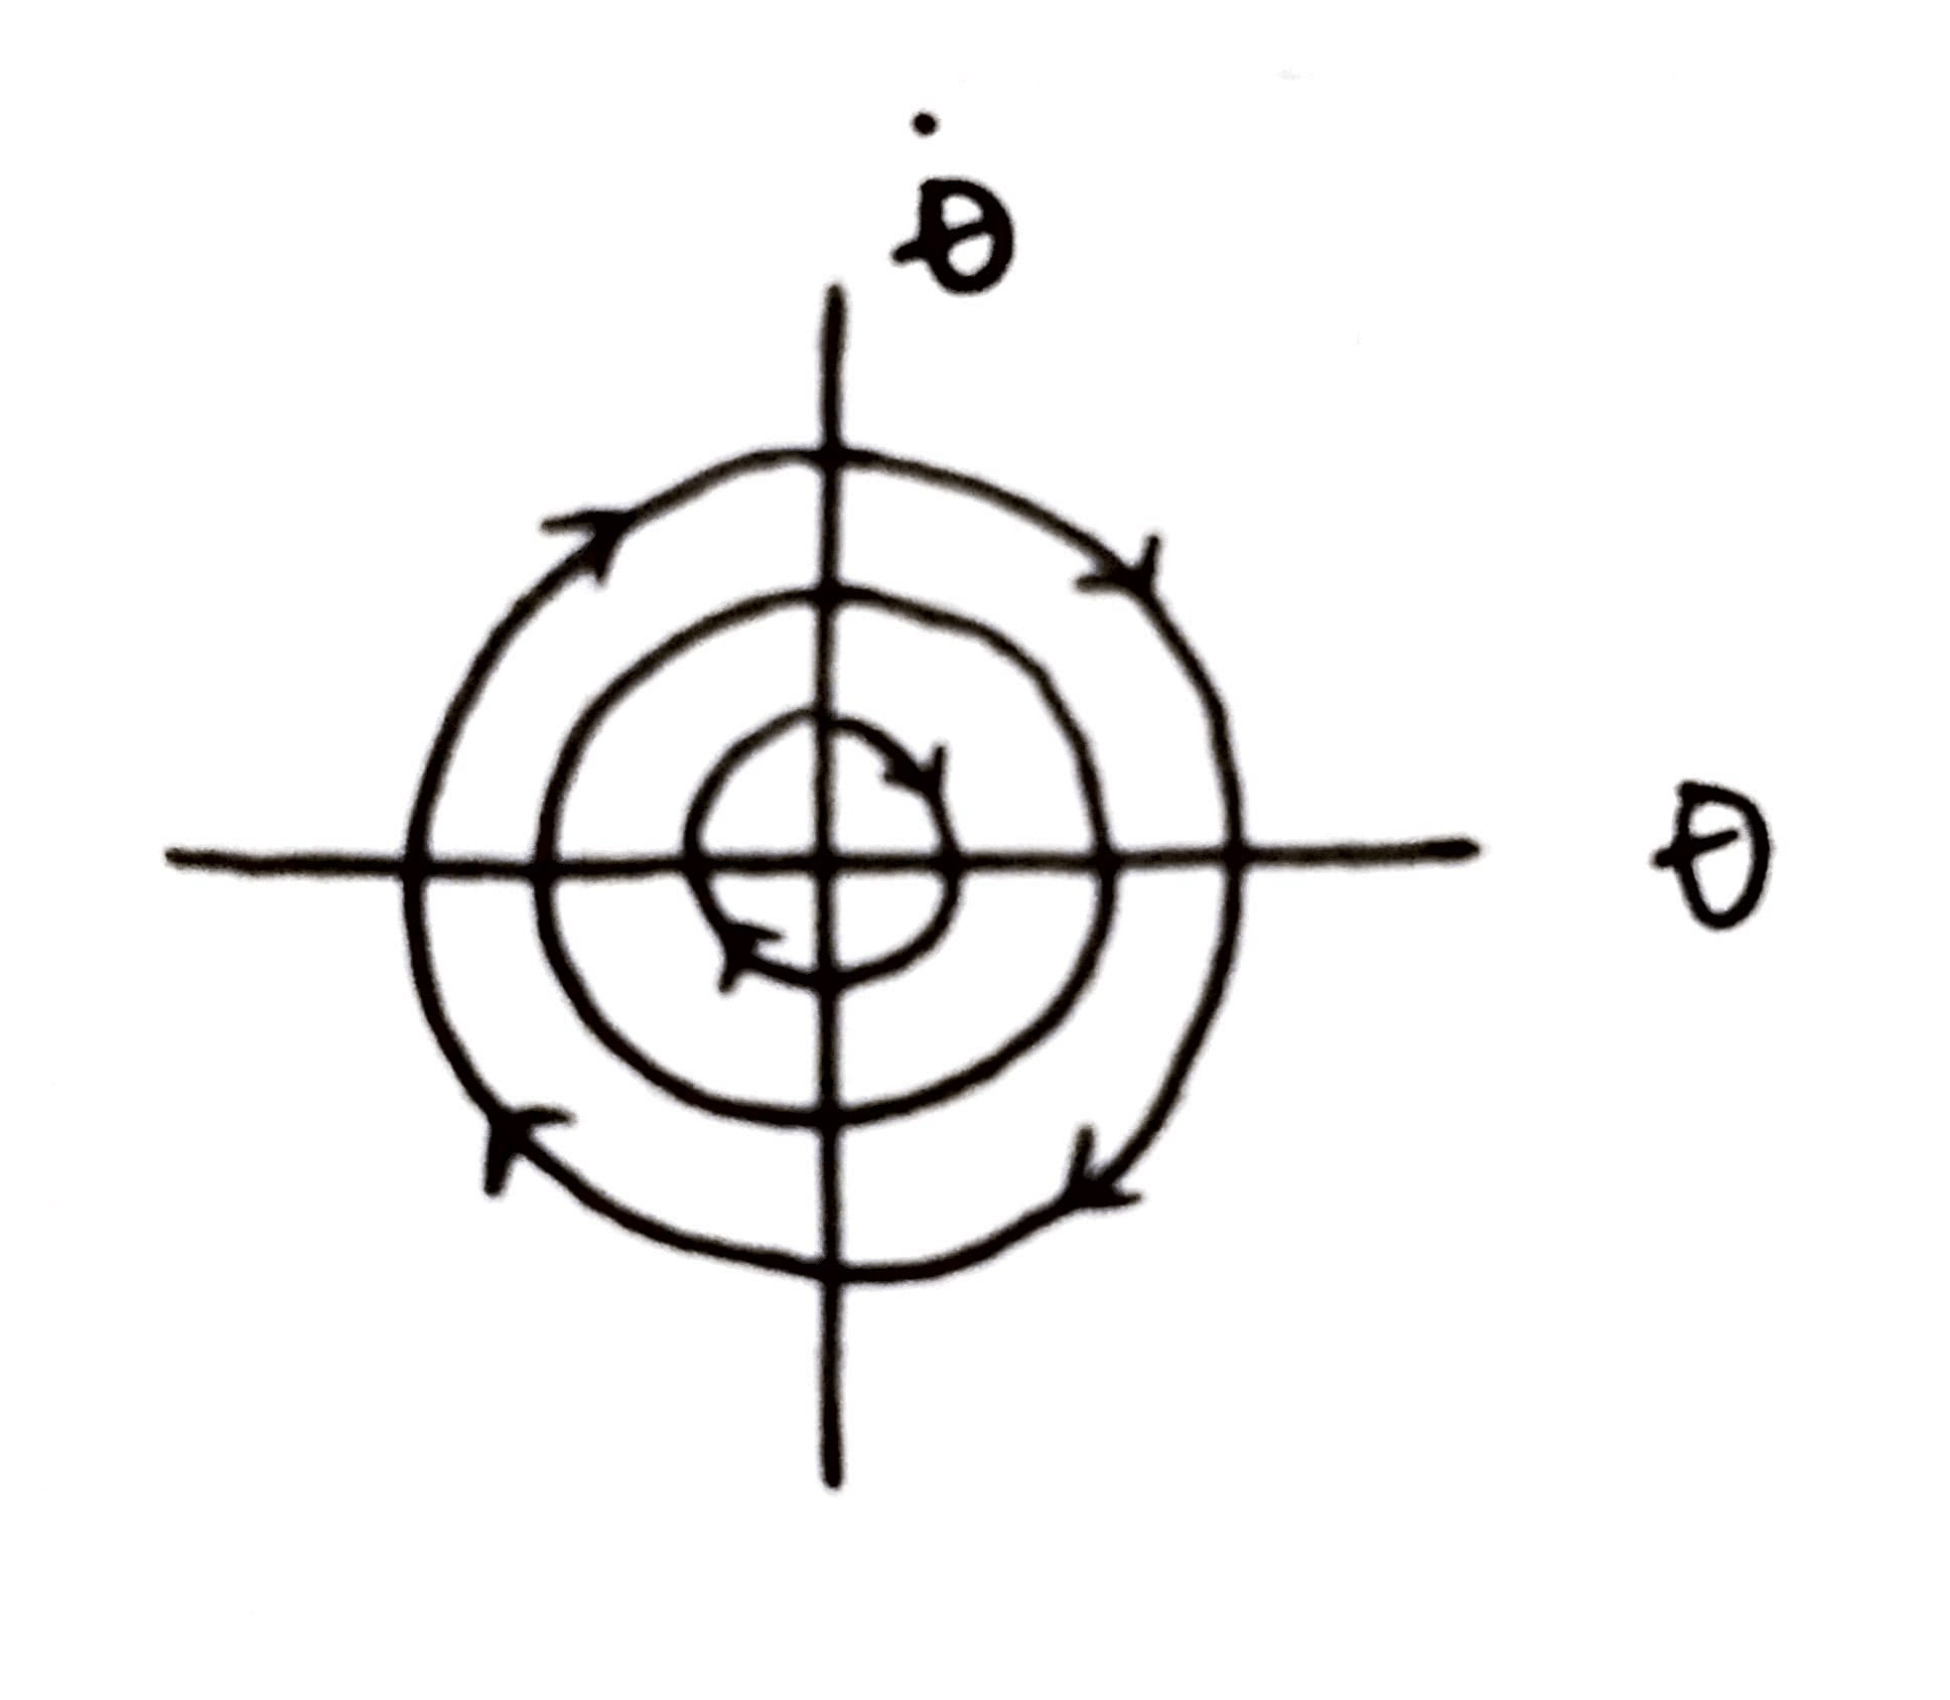
\includegraphics[height=0.2\textwidth]{img/2019S1-4.png}
        \end{center}
        
        After our bifurcation, we have 3 fixed points. Our inner fixed point at $(\theta, \dot\theta) = (0, 0)$ is unstable (and therefore a saddle) and our outer two are stable (centers), and so our phase portrait is as follows:
        
        \begin{center}
        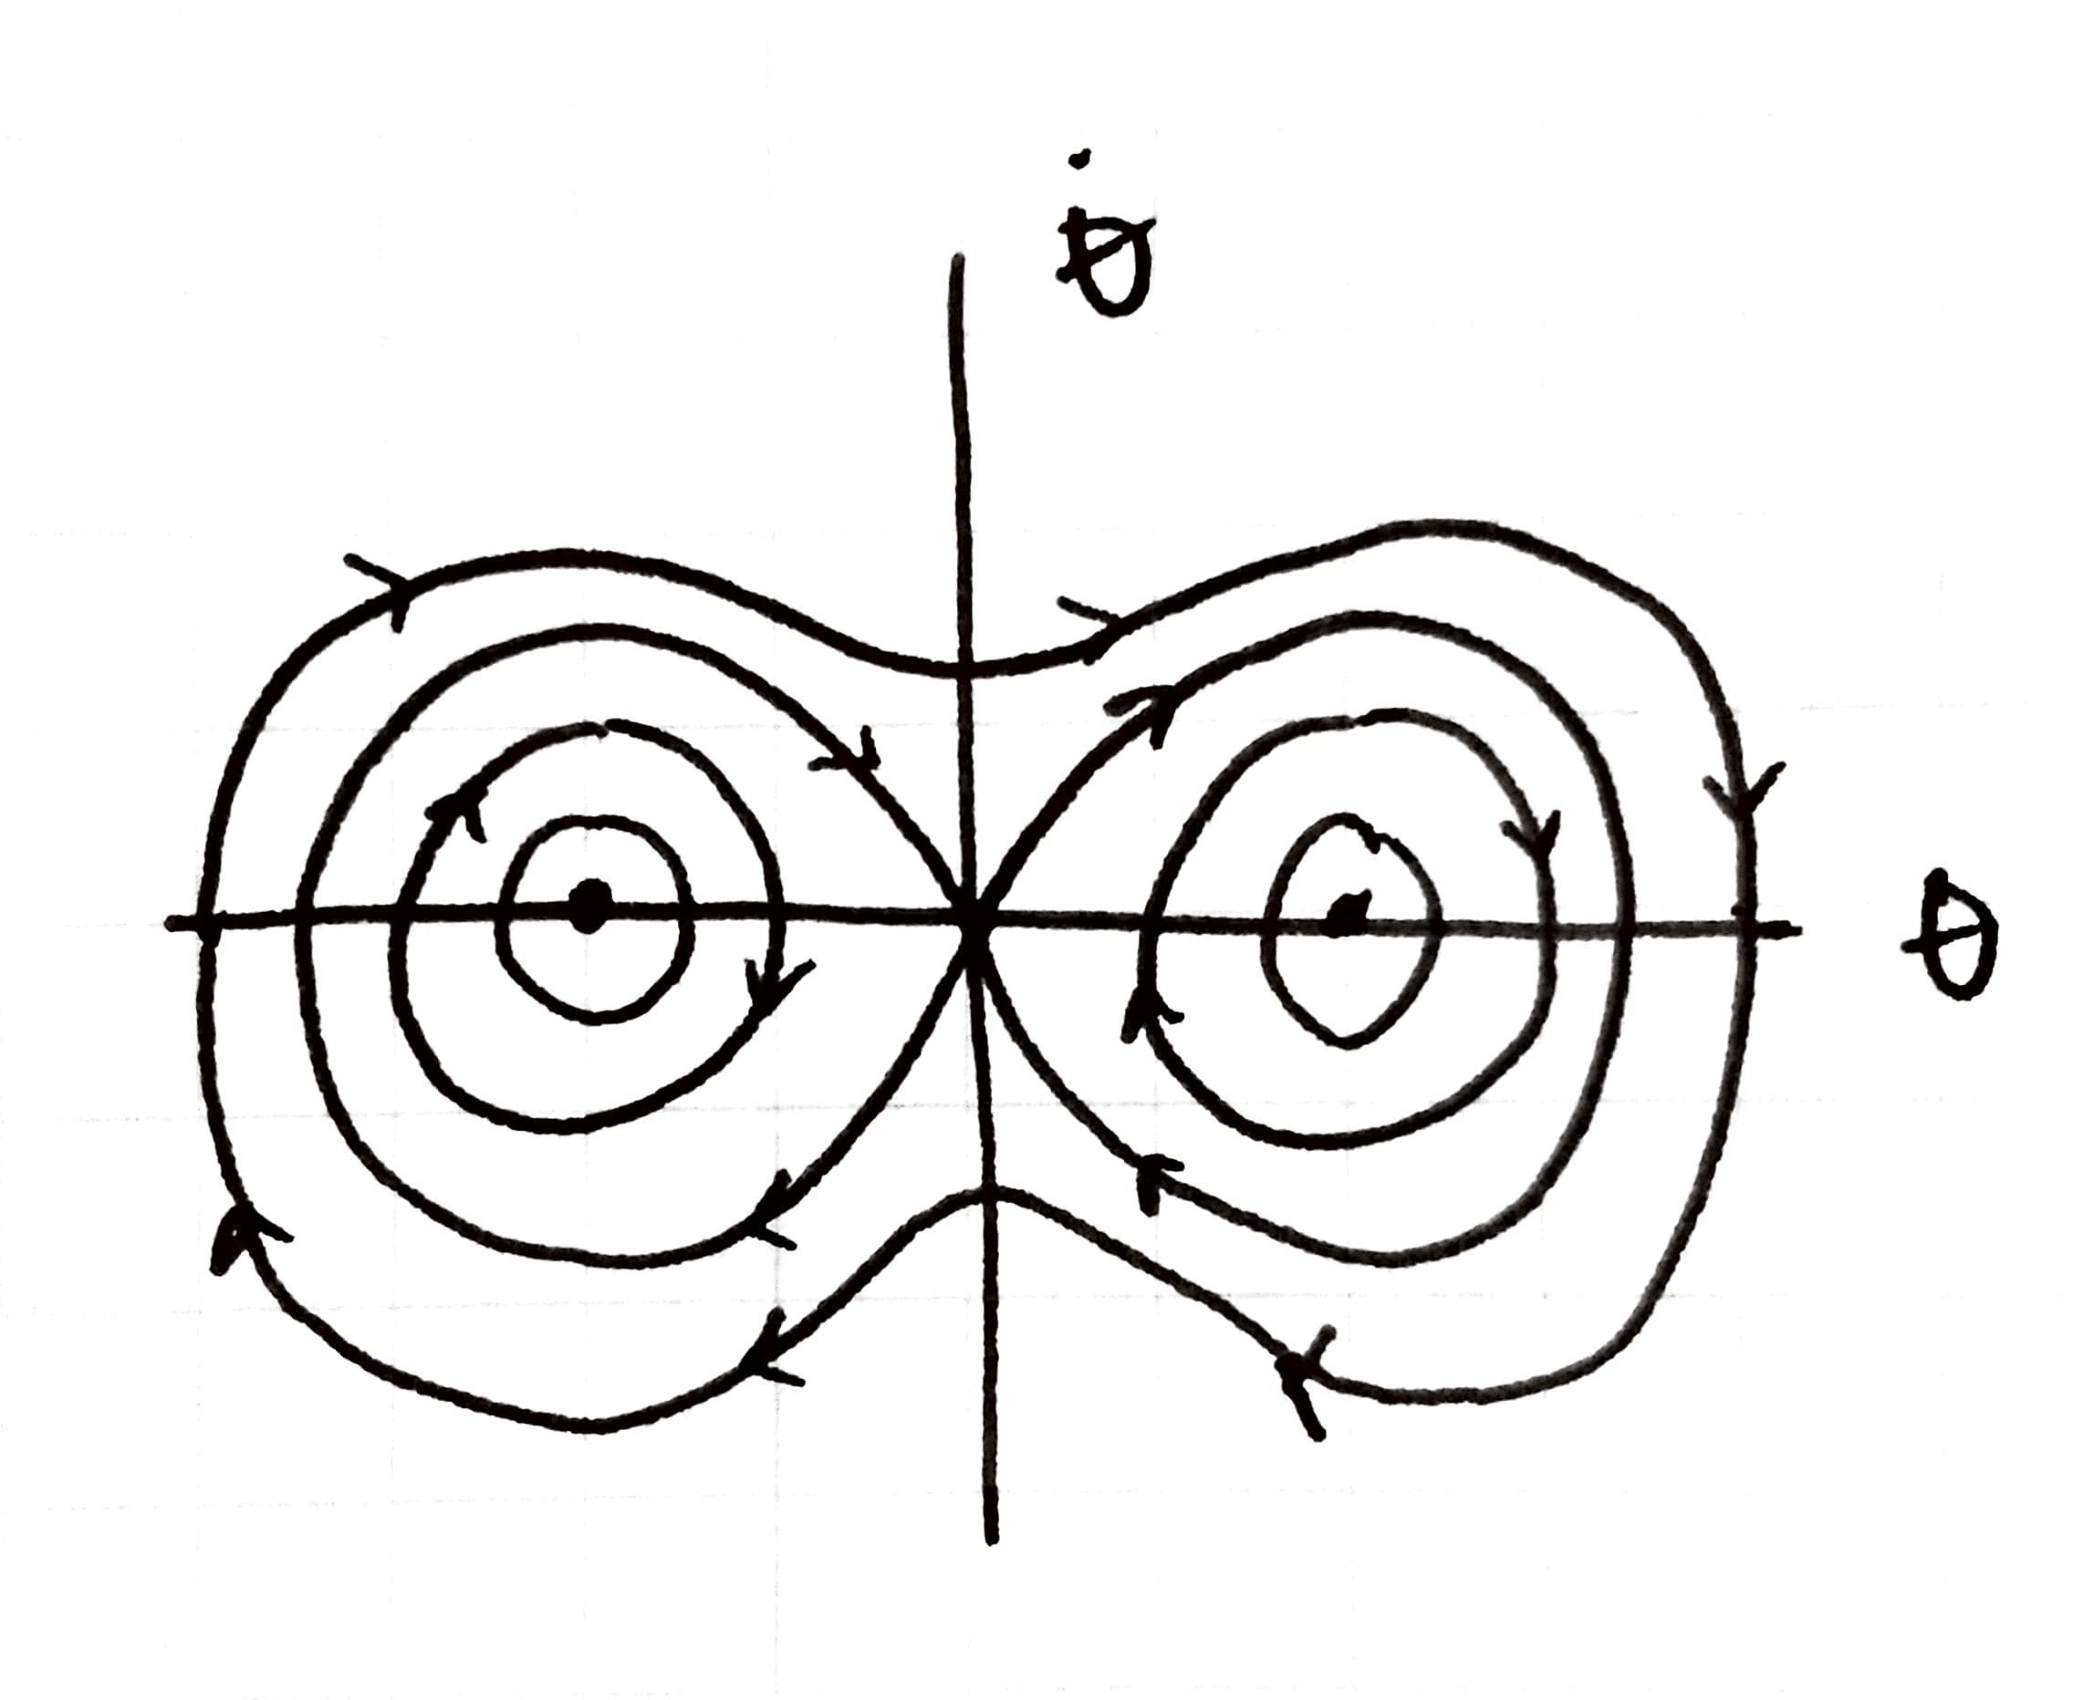
\includegraphics[height=0.2\textwidth]{img/2019S1-5.png}
        \end{center}
    \end{enumerate}
    
    \item
    \begin{qbox}
    Consider the following predator-prey model:
    \[
    \frac{dx}{dt} = x(x(1-x) - y), \qquad \frac{dy}{dt} = y(x - a),
    \]
    where $x$ is the (positive) non-dimensional population of prey, $y$ is the (positive) non-dimensional population of predators, and $a$ is a (positive) non-dimensional parameter.
    
    \begin{itemize}
        \item[\textbf{(a)}] Sketch the nullclines in the first quadrant, $x, y \geq 0$.
        \item[\textbf{(b)}] Find and classify all fixed points.
        \item[\textbf{(c)}] Find and classify all bifurcations that occur as a varies (assume $a > 0$).
        \item[\textbf{(d)}] Show that a stable limit cycle exists for some values of $a$.
    \end{itemize}
    \end{qbox}
    
    \begin{enumerate}
    \item
    Our $x$-nullclines are where $\dot x = 0$: this occurs when $x = 0$ or $y = x(1-x)$.
    
    Our $y$-nullclines are $x = a$ or $y = 0.$
    
    \begin{center}
    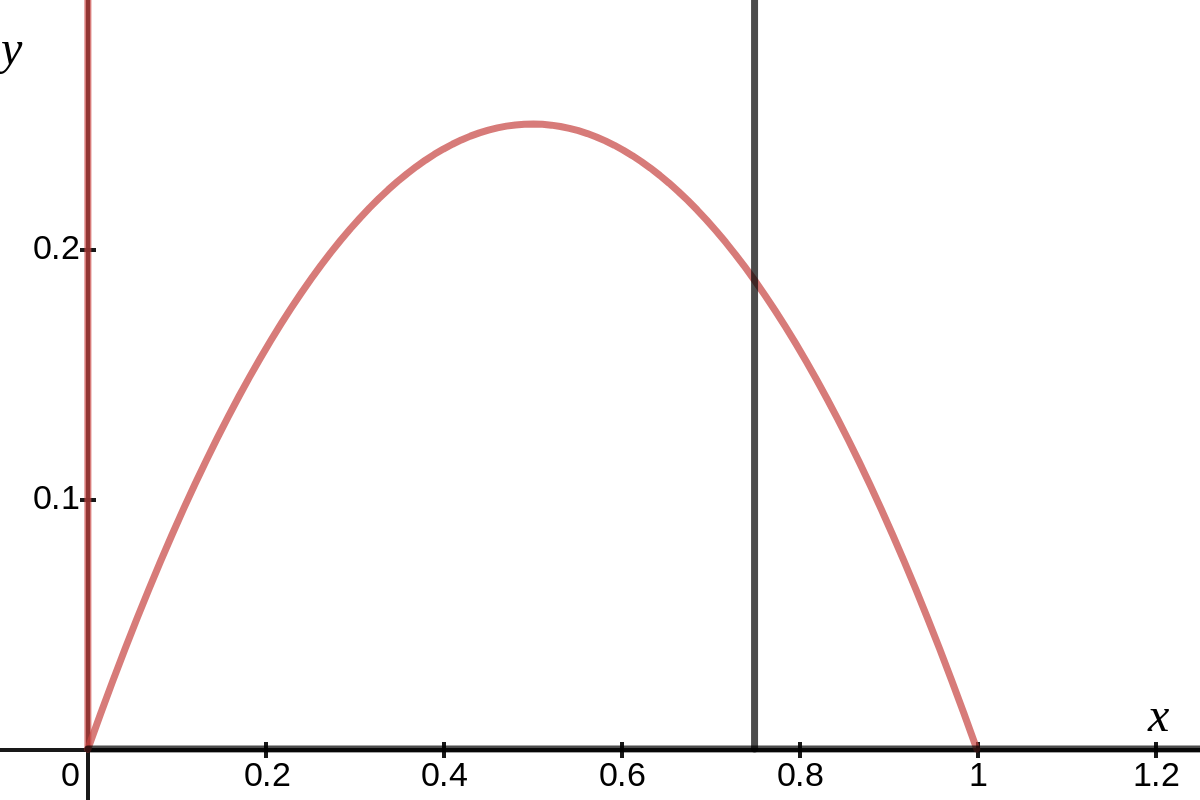
\includegraphics[height=0.3\textwidth]{img/2019S2-1.png}
    \end{center}
    
    \item We have a total of 2, sometimes 3, fixed points. Two fixed points which we always have are $(x, y) = (0, 0)$ and $(1, 0)$. When $a \leq 1$, we have the additional fixed point $(a, a(1 - a))$.
    
    To classify our fixed points, we first compute the Jacobian.
    \[
    J = \mtx{cc}{-3x^2 + 2x - y & -x \\ y & x - a}.
    \]
    First, we examine (0, 0).
    \[
    J\big\vert_{(0, 0)} = \mtx{cr}{0 & 0 \\ 0 & -a}
    \]
    The eigenvalues are $-a$ and $0$, so linear stability analysis fails. However, we do know that since $a > 0$, that $(0, 0)$ must be either a saddle point or a stable node. Graphically, along the line $y = 0$ close to $(0, 0)$, the flow in the $x$-direction is positive, and so this point must be a saddle.
    
    Now, we examine $(1, 0)$.
    \[
    J\big\vert_{(1, 0)} = \mtx{rc}{-1 & 0 \\ 0 & 1 - a}
    \]
    Our eigenvalues are $-1$ and $1 - a$, so this point is a saddle point if $a < 1$ and a stable node if $a > 1.$
    
    Finally, we examine $(a, a(1 - a))$:
    \[
    J\big\vert_{(a, a(1 - a))} = \mtx{cr}{-3a^2 + 2a - a(1 - a) & -a \\ a(1 - a) & 0} = \mtx{cr}{a(1 - 2a) & -a \\ a(1 - a) & 0}
    \]
    Its characteristic equation is
    \[
    \lambda^2 - a(1 - 2a)\lambda + a^2(1 - a) = 0
    \]
    which gives eigenvalues
    \[
    \lambda = \frac{1}{2}\left(a(1 - 2a) \pm \sqrt{a^2(1 - 2a)^2 - 4a^2(1 - a)}\right) = \frac{1}{2}\left(a(1 - 2a) \pm a\sqrt{4a^2 - 3}\right).
    \]
    These eigenvalues are complex when $4a^2 - 3 < 0$, that is, $a < \sqrt{3}/2$. In this situation, they have positive real part for $1 - 2a > 0$, that is, $a < 1/2$, and negative real part for $a > 1/2$. Finally, in the case where our eigenvalues are real, we must have $a > \sqrt{3}/2 > 1/2$, and so $a(1 - 2a)$ is negative. In this case, one of our eigenvalues will always be negative. The other will be positive when
    \begin{align*}
        a(1 - 2a) + a\sqrt{4a^2 - 3} &> 0
        \\
        a\left((1 - 2a) + \sqrt{4a^2 - 3}\right) &> 0
        \\
        1 - 2a + \sqrt{4a^2 - 3} &> 0
        \\
        \sqrt{4a^2 - 3} &> 2a - 1
        \\
        4a^2 - 3 &> 4a^2 - 4a + 1
        \\
        a &> 1.
    \end{align*}
    So, the fixed point $(a, a(1-a))$ is classified as:
    \[
    \begin{cases}
    \textrm{unstable spiral} &a < 1/2 \\
    \textrm{stable spiral} &1/2 < a < \sqrt{3}/2 \\
    \textrm{stable node} &\sqrt{3}/2 < a < 1 \\
    \textrm{saddle} &a > 1
    \end{cases}
    \]
    
    \item When $a$ passes through 1, we get a transcritical bifurcation as the points $(a, (a(1-a))$ and $(1, 0)$ swap stability. 
    
    When $a$ passes through $1/2$, we have a Hopf bifurcation as the stability of $(a, a(1 - a))$ swaps. When we go from a stable spiral to an unstable spiral, a stable limit cycle must appear, and so this Hopf bifurcation is supercritical.
    
    \item As shown in previous parts, due to the fact we have a Hopf bifurcation at $a = 1/2$ and since the point $(a, a(1-a))$ is an unstable spiral when $a < 1/2$, we have a stable limit cycle in this region.
    
    \end{enumerate}
    
    \item
    \begin{qbox}
    An annular plate with inner and outer radii $a < b$, respectively, is held at temperature $B$ at its outer boundary and satisfies the boundary condition $\partial u/ \partial r = A$ at its inner boundary, where $A,B$ are constants. Find the temperature if it is at a \textit{steady state.}
    
    \textit{Hint}: It satisfies the two-dimensional Laplace equation and depends only on $r$. You can also use the fact that the Laplace operator can be expressed in the polar coordinate $(r,\theta)$ as:
    \[\Delta = \frac{d^2}{dr^2} + \frac{1}{r}\frac{d}{dr} + \frac{1}{r^2}\frac{d^2}{d\theta^2}.
    \]
    \end{qbox}
    
    The equation we need to solve is $\Delta u = 0$. Since $u$ is not dependant on $\theta$, we may rewrite this as
    \[
    u_{rr} + \frac{1}{r}u_r = 0.
    \]
    We define $w(r) = u_r$. Now, we wish to solve the equation
    \[
    w'(r) + \frac{1}{r}w(r) = 0.
    \]
    This is a separable differential equation:
    \begin{align*}
        \frac{dw}{w} &= -\int \frac{dr}{r}
        \\
        \ln w &= -\ln r + C
        \\
        w &= \frac{c_1}{r}
    \end{align*}
    Now, we solve for $u$:
    \begin{align*}
        u'(r) &= \frac{c_1}{r}
        \\
        u(r) &= c_1\ln r + c_2
    \end{align*}
    We plug in our boundary conditions to solve for $c_1,c_2$. The inner boundary condition $u_r(a) = A$ gives:
    \begin{align*}
        A = \frac{c_1}{a} \qquad \rightarrow \qquad c_1 = Aa.
    \end{align*}
    So, our equation becomes
    \[
    u(r) = Aa\ln r + c_2.
    \]
    Our second boundary condition $u(b) = B$ gives
    \[
    B = Aa \ln b + c_2 \qquad \rightarrow \qquad c_2 = B - Aa\ln b.
    \]
    So, our solution is given by
    \[
    u(r,\theta) = Aa\ln\left(\frac{r}{b}\right) + B.
    \]
    
\item \begin{qbox}
Let $\omega$ be positive, but not an integer multiple of $\pi$, and consider the following boundary value problem on the unit interval $[0, 1]:$
\[
f'' + \omega^2 f = g, \qquad f'(0) = 0 = f'(1).
\]
\begin{itemize}
    \item[\textbf{(a)}] Find the Green's function for this boundary value problem.
    \item[\textbf{(b)}] Discuss what happens if we try this with $\omega = 0$.
\end{itemize}
\end{qbox}
\begin{enumerate}
    \item The homogeneous version of the problem is given by
    \[
    f'' = -\omega^2 f,
    \]
    which has solutions of the form 
    \begin{align*}
    f &= A \sin(\omega x) + B\cos(\omega x)
    \\
    f' &= A \cos(\omega x) - B\sin(\omega x)
    \end{align*}
    Plugging in the left boundary condition gives $A = 0$, so our fist solution is
    \[
    f_1 = \cos(\omega x).
    \]
    
    % we have
    % \begin{align*}
    %     f_0 = B\cos(\omega x).
    % \end{align*}
    % To solve for $B$, we integrate over the interval $x \in [0, 1]:$
    % \begin{align*}
    %     1 &= B\int_0^1 \cos(\omega x)\,dx \\
    %     1 &= B\left[\frac{\sin(\omega x)}{\omega}\right]_0^1 \\
    %     1 &= B \frac{\sin \omega}{\omega}
    %     \\
    %     B &= \frac{\omega}{\sin \omega}.
    % \end{align*}
    % So, our left solution is
    % \[
    % f_0 = \frac{\omega}{\sin \omega} \cos(\omega x).
    % \]
    Now, we plug in the right boundary condition. This yields
    \begin{align*}
        A \cos \omega - B\sin\omega &= 0
        \so
        B = A \frac{\cos \omega}{\sin \omega}
    \end{align*}
    So our second solution is
    \[
    f_2 = \sin(\omega x) + \frac{\cos \omega}{\sin \omega}\cos(\omega x)
    \]
    % Integrating over $x \in [0, 1]$ to solve for $A$, we get
    % \begin{align*}
    %     1 &= A\int_0^1 \left[\sin(\omega x) + \frac{\cos \omega}{\sin \omega}\cos(\omega x)\right]\,dx
    %     \\
    %     1 &= A\left[ -\frac{1}{\omega}\cos(\omega x) + \frac{\cos \omega}{\omega \sin \omega}\sin(\omega x) \right]_0^1
    %     \\
    %     1 &= A\left[ -\frac{1}{\omega}\cos \omega + \frac{\cos \omega}{\omega \sin \omega}\sin \omega + \frac{1}{\omega} \right]
    %     \\
    %     A &= \omega
    % \end{align*}
    % So, our right solution is
    % \[
    % f_1 = \omega \left(\sin(\omega x) + \frac{\cos \omega}{\sin \omega}\cos(\omega x)\right).
    % \]
    Our Green's function then has the form
    \[
    G(x, \xi) = \begin{cases}
    \frac{1}{c}f_1(x)f_2(\xi) &: x \leq \xi \\
    \frac{1}{c}f_1(\xi)f_2(x) &: x \geq \xi
    \end{cases}
    \]
    where $c = pw$, $p = 1$ for this problem, and $w$ is the Wronskian
    \begin{align*}
        w &= \det \mtx{cc}{f_1 & f_2 \\ f_1' & f_2'} \\
        &= \det \mtx{cc}{ \cos(\omega x) & \sin(\omega x) + \frac{\cos \omega}{\sin \omega}\cos(\omega x) \\ -\omega \sin(\omega x) & \omega \cos(\omega x) - \frac{\omega\cos \omega}{\sin \omega}\sin(\omega x)}
        \\
        &=
        \omega \cos^2(\omega x) - \frac{\omega \cos \omega}{\sin \omega}\cos(\omega x)\sin(\omega x) + \omega \sin^2(\omega x) + \frac{\omega \cos \omega}{\sin \omega} \cos(\omega x)\sin(\omega x)
        \\
        &= \omega.
    \end{align*}
    So, our Green's function is given by
    \[
    G(x, \xi) = \begin{cases}
    \frac{1}{\omega}\cos(\omega x)\left(\sin(\omega \xi) + \frac{\cos \omega}{\sin \omega}\cos(\omega \xi)\right) 
    &: x \leq \xi 
    \\
    \frac{1}{\omega}\cos(\omega \xi)\left(\sin(\omega x) + \frac{\cos \omega}{\sin \omega}\cos(\omega x)\right) 
    &: x \geq \xi
    \end{cases}
    \]
    \item If $\omega = 0$, then our homogeneous problem is simply $f'' = 0$, which has solutions of the form
    \[
    f(x) = Ax + B.
    \]
    Imposing either boundary condition leads to $A = 0$, and so our left and right equations (and thus our Green's function) are constant.
\end{enumerate}

\item \begin{qbox}
Let $A$ be a symmetric matrix and let $\lambda_0$ be a simple (i.e. multiplicity one) eigenvalue of $A$ with corresponding eigenvector $\bvec v_0$. Derive an expression for the eigenvalue, $\lambda$, up to
order $\epsilon$ in the limit of small $\epsilon$ to the problem
\[
A\bvec v + \epsilon \bvec F(\bvec v) = \lambda \bvec v
\]
that is $\lambda_0$ at leading order.
\end{qbox}

We assume $\bvec v \thicksim \bvec v_0 + \epsilon \bvec v_1$ and $\lambda \thicksim \lambda_0 + \epsilon \lambda_1$. Then, our equation becomes
\begin{align*}
    A(\bvec v_0 + \epsilon \bvec v_1) + \epsilon \bvec F(\bvec v_0 + \epsilon \bvec v_1) &= (\lambda_0 + \epsilon \lambda_1) (\bvec v_0 + \epsilon \bvec v_1)
\end{align*}
Our leading-order equation is
\[
A\bvec v_0 = \lambda_0 \bvec v_0.
\]
Next, our $\Ord{\epsilon}$ equation is
\begin{align*}
    A\bvec v_1 + \bvec F(\bvec v_0) &= \lambda_0 \bvec v_1 + \lambda_1 \bvec v_0.
\end{align*}
Since $A$ is symmetric, we use the fact that its eigenvectors are orthogonal. So, our $\Ord{\epsilon}$ equation becomes:
\begin{align*}
    A\bvec v_1 + \bvec F(\bvec v_0) &= \lambda_0 \bvec v_1 + \lambda_1 \bvec v_0
    \\
    \bvec v_0^\intercal A\bvec v_1 + \bvec v_0^\intercal \bvec F(\bvec v_0) &= \lambda_0 \bvec v_0^\intercal \bvec v_1 + \lambda_1 \bvec v_0^\intercal \bvec v_0 \\
    \left(A \bvec v_0\right)^\intercal \bvec v_1 + \bvec v_0^\intercal \bvec F(\bvec v_0) &= \lambda_0 \bvec v_0^\intercal \bvec v_1 + \lambda_1 \bvec v_0^\intercal \bvec v_0
    \\
    \lambda_0 \bvec v_0^\intercal \bvec v_1 + \bvec v_0^\intercal \bvec F(\bvec v_0) &= \lambda_0 \bvec v_0^\intercal \bvec v_1 + \lambda_1 \bvec v_0^\intercal \bvec v_0
    \\
    \bvec v_0^\intercal \bvec F(\bvec v_0) &= \lambda_1 \bvec v_0^\intercal \bvec v_0
    \\
    \lambda_1 &= \frac{\bvec v_0^\intercal \bvec F(\bvec v_0)}{\bvec v_0^\intercal \bvec v_0}.
\end{align*}

\item \begin{qbox}
The van der Pol oscillator,
\begin{align*}
    \epsilon \dot u &= v + u - \frac{u^3}{3} \\
    \dot v &= - u
\end{align*}
exhibits periodic relaxation oscillations. The oscillation exhibits two time scales (a fast and slow time scale) for small $\epsilon$.

Let $f(u) = u^3 /3 - u$. The following information about $f$ may be helpful:
\begin{align*}
    f'(\pm 1) &= 0 \\
    f(\pm 1) &= \mp 2/3 \\
    f(\pm 2) &= \pm 2/3
\end{align*}
\begin{itemize}
\item[\textbf{(a)}] Draw the nullclines in the phase plane ($uv$-plane), sketch the the limit cycle for small $\epsilon$, and label the regions of fast and slow dynamics on the limit cycle.
\item[\textbf{(b)}] Compute the period of the oscillation at leading order as $\epsilon \to 0$.
\end{itemize}
\end{qbox}

\begin{enumerate}
    \item Setting $\dot v = 0$ gives the $v$-nullcline $u = 0$. Along this line, we have $\dot u = v/\epsilon$, which is very large for $\epsilon \ll 1$. Next, setting $\dot u = 0$ gives the $u$-nullcline $v = f(u) = u^3/3 - u = u/3 \cdot (u + \sqrt 3)(u - \sqrt 3)$, which has zeros at $u = 0, \pm \sqrt 3$. Along this line, $\dot v$ has the opposite sign as $u$, and is generally small compared to the motion along the $v$-nullcline. This yields the following images of the phase plane, for the nullclines and the limit cycle respectively:
    
    \begin{center}
    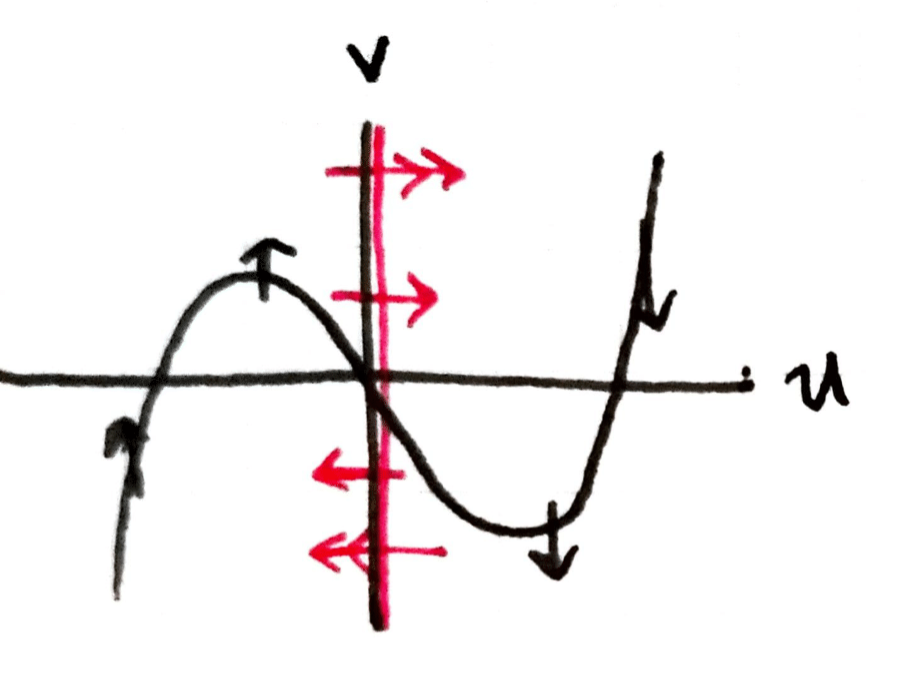
\includegraphics[height=0.3\textwidth]{img/2019S6a1.png} \qquad 
    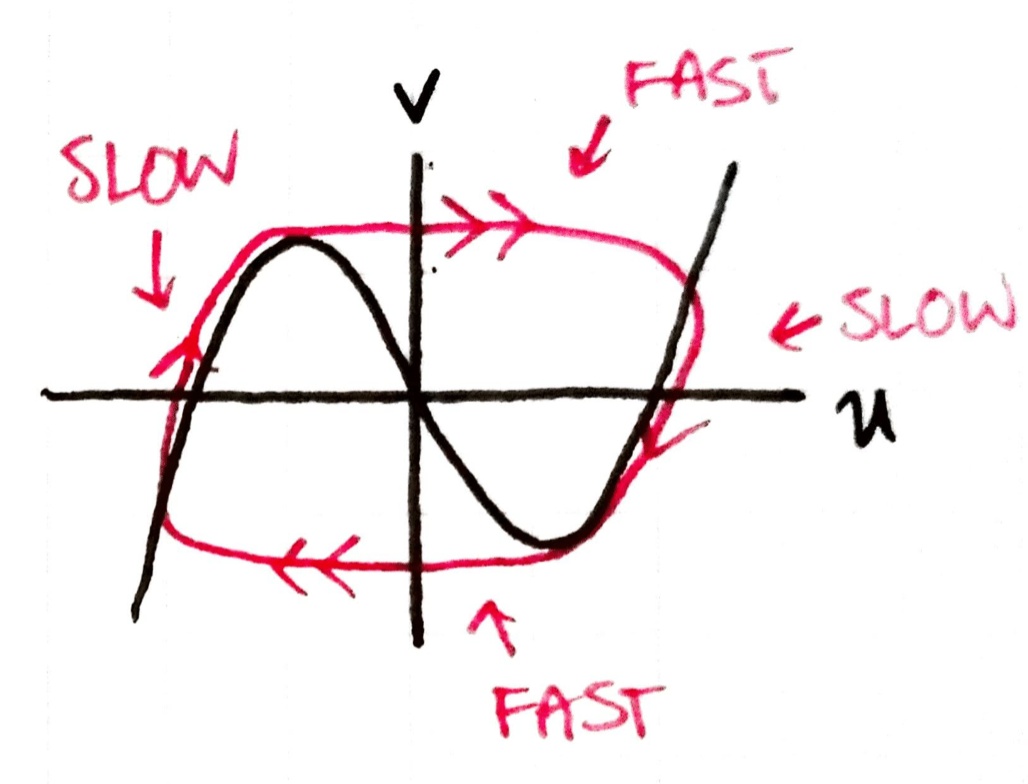
\includegraphics[height=0.3\textwidth]{img/2019S6a2.png}
    \end{center}
    
\end{enumerate}

\end{enumerate}

\chapter*{Fall 2018}
\chaptermark{Fall 2018}
\addcontentsline{toc}{chapter}{Fall 2018}

\begin{enumerate}

\item 
\begin{qbox}
Suppose a bead of mass $m$ slides frictionlessly on a hoop of radius $R$. If we then spin the hoop at constant angular velocity $\omega$ about an axis parallel to the force of gravity (see Fig. 1), the bead obeys the following non-linear second order differential equation:
\[
\frac{d^2\theta}{dt^2} - \omega^2 \sin\theta \cos\theta + \frac{g}{R}\sin\theta = 0,
\]
where $g$ is the acceleration of gravity, $\theta(t)$ is the bead's angular position on the hoop (with
$\theta = 0$ being at the bottom), and $t$ is time.

\begin{itemize}
    \item[\textbf{(a)}] Use non-dimensionalization to show that the qualitative behavior of the system is defined by a single non-dimensional parameter.
    
    \item[\textbf{(b)}] Find all fixed points, determine their stability and classify them as a function of that parameter.
    
    \item[\textbf{(c)}] Sketch a bifurcation plot (i.e., sketch the fixed points as a function of the parameter, indicate the stability of the fixed points, and label any bifurcations that occur). Use the Lyapunov definition of stability for this part.
    
    It may or may not be useful to know that the energy of the system can be written as
    \[
    E = mg (R - R\cos\theta) + \frac{m}{2}\left(R^2 \sin^2\theta + R^2 \left(\frac{d\theta}{dt}\right)^2\right).
    \]
    The Lyapunov definition of stability is that a fixed point is stable if all trajectories starting sufficiently close to the fixed point remain within an arbitrarily small distance of the fixed point.
\end{itemize}
\end{qbox}

\begin{enumerate}
    \item We examine the dimensions of our given parameters:
    \[
    [\omega] = \frac{1}{T} \qquad [g] = \frac{L}{T^2} \qquad [R] = L
    \]
    Since $\theta$ is dimensionless, we only need to nondimensionalize $t$. We define the characteristic timescale $t_c$ and let $\widetilde t$ be the dimesionless value such that $t = t_c\widetilde t$. Then our equation becomes
    \begin{align*}
        \frac{1}{t_c^2} \frac{d^2\theta}{d\widetilde t^2} - \omega^2 \sin\theta \cos\theta + \frac{g}{R}\sin\theta 
        &= 
        0
        \\
        \frac{d^2\theta}{d\widetilde t^2} - \omega^2 t_c^2 \sin\theta \cos\theta + \frac{g}{R}t_c^2\sin\theta 
        &= 
        0
    \end{align*}
    Since $\omega$ may be 0, we avoid using it in our characteristic timescale and instead let $t_c^2 = R/g$. We verify that this has units of time:
    \[
    [t_c] = \sqrt{\frac{L}{L/T^2}} = T
    \]
    Returning to our equation, we now have
    \begin{align*}
        \frac{d^2\theta}{d\widetilde t^2} - \frac{\omega^2R}{g} \sin\theta \cos\theta + \sin\theta 
        &= 
        0.
    \end{align*}
    We define the parameter $\mu = \omega^2R/g$ and verify that it's dimensionless:
    \[
    [\mu] = \frac{1/T^2 \cdot L}{L/T^2} = 1
    \]
    So, our dimensionless equation (dropping our tildes) is
    \[
    \ddot \theta = \mu\sin\theta\cos\theta - \sin\theta.
    \]
    
    \item We reduce our second-order ODE to a system of two first-order ODEs:
    \[
    \begin{cases}
    \: \dot \theta = \psi \\
    \dot \psi = \mu \sin\theta\cos\theta - \sin\theta = \sin\theta(\mu\cos\theta - 1)
    \end{cases}
    \]
    We will choose the range of $\theta$ as $\theta \in (-\pi, \pi]$. Our first equation is only zero when $\psi = \dot\theta = 0$. Our second equation is zero whenever $\sin\theta = 0$ (which is when $\theta = 0, \pi$) or when $\cos\theta = 1/\mu$, which occurs for $\theta = \pm\cos^{-1}(1/\mu)$. 
    So, our fixed points are $(\theta, \dot \theta ) = (0, 0), (\pi, 0),$ and $(\pm\cos^{-1}(1/\mu), 0)$, noting that the last pair of fixed points only exists for $\mu \geq 1$.
    
    To find their linear stability, we compute the Jacobian.
    \[
    J = \mtx{cc}{0 & 1 \\ \mu\left(\cos^2\theta -\sin^2\theta\right) - \cos\theta & 0}.
    \]
    First, we examine (0, 0). In this case, our Jacobian becomes
    \[
    J\big\vert_{(0, 0)} = \mtx{cc}{0 & 1 \\ \mu - 1 & 0} \qquad \rightarrow \qquad \lambda^2 - (\mu - 1) = 0 \qquad \rightarrow \qquad \lambda = \pm \sqrt{\mu - 1}
    \]
    So, we have the following classification:
    \[
    (0, 0) \textrm{ is a } \begin{cases}
    \textrm{saddle (unstable)} &\mu > 1 \\
    \textrm{linear center (linearly stable)} &0 \leq \mu < 1
    \end{cases}
    \]
    Next, we examine $(\pi, 0)$. Now, our Jacobian becomes
    \[
    J\big\vert_{(\pi, 0)} = \mtx{cc}{0 & 1 \\ \mu + 1 & 0} \qquad \rightarrow \qquad \lambda^2 - (\mu + 1) = 0 \qquad \rightarrow \qquad \lambda = \pm \sqrt{\mu + 1}
    \]
    Since $\mu \geq 0$ always, we have $(\pi, 0)$ is a saddle point and thus unstable.
    
    Finally, we examine $(\pm \cos^{-1}(1/\mu), 0)$. We use the trig identity $\sin(\cos^{-1}(x)) = \sqrt{1 - x^2}$.
    \[
    J\big\vert_{(\pm \cos^{-1}(1/\mu), 0)} = \mtx{cc}{0 & 1 \\ \mu\left(1/\mu^2 - (1 - 1/\mu^2)\right) - 1/\mu & 0} = \mtx{cc}{0 & 1 \\ 1/\mu - \mu & 0} 
    \]
    Our eigenvalues are therefore $\lambda = \pm \sqrt{1/\mu - \mu}$. Since this pair of fixed points only occurs for $\mu \geq 1$, the expression under our radical is always negative (except when $\mu = 1$ exactly, in which case we have zero eigenvalues). So, we have a linear center (and thus linearly stable) when $\mu > 1$. When $\mu = 1$, it is unclassifiable. 
    
    \item If our system is a conservative system, then linear center will be true centers and therefore Lyapunov stable. So, we show that there exists a conserved quantity. I was unable to find a conserved quantity using the given expression for the total energy of the system, but using the original ODE, we get
    \begin{align*}
        \ddot \theta &= \omega^2 \sin\theta\cos\theta - \frac{g}{R}\sin\theta \\
        \ddot \theta \dot\theta &= \left(\omega^2 \sin\theta\cos\theta - \frac{g}{R}\sin\theta\right)\dot\theta
        \\
        \frac{d}{dt}\left[\frac{\dot\theta^2}{2}\right] 
        &=
        \frac{d}{dt}\left[\frac{\omega^2}{2}\sin^2\theta + \frac{g}{R}\cos\theta\right]
        \\
        \frac{\dot\theta^2}{2}
        &=
        \frac{\omega^2}{2}\sin^2\theta + \frac{g}{R}\cos\theta + C
        \\
        \frac{\dot\theta^2}{2} - \frac{\omega^2}{2}\sin^2\theta - \frac{g}{R}\cos\theta
        &=
        C
    \end{align*}
    
    So we have a conserved quantity, and therefore our system is conservative. So, our linear centers are Lyapunov stable.
    
    Since $\dot \theta = 0$ for each of our fixed points and is unaffected by $\mu$, we draw a two-dimensional bifurcation diagram in $\mu$ and $\theta$ alone:
    \begin{center}
    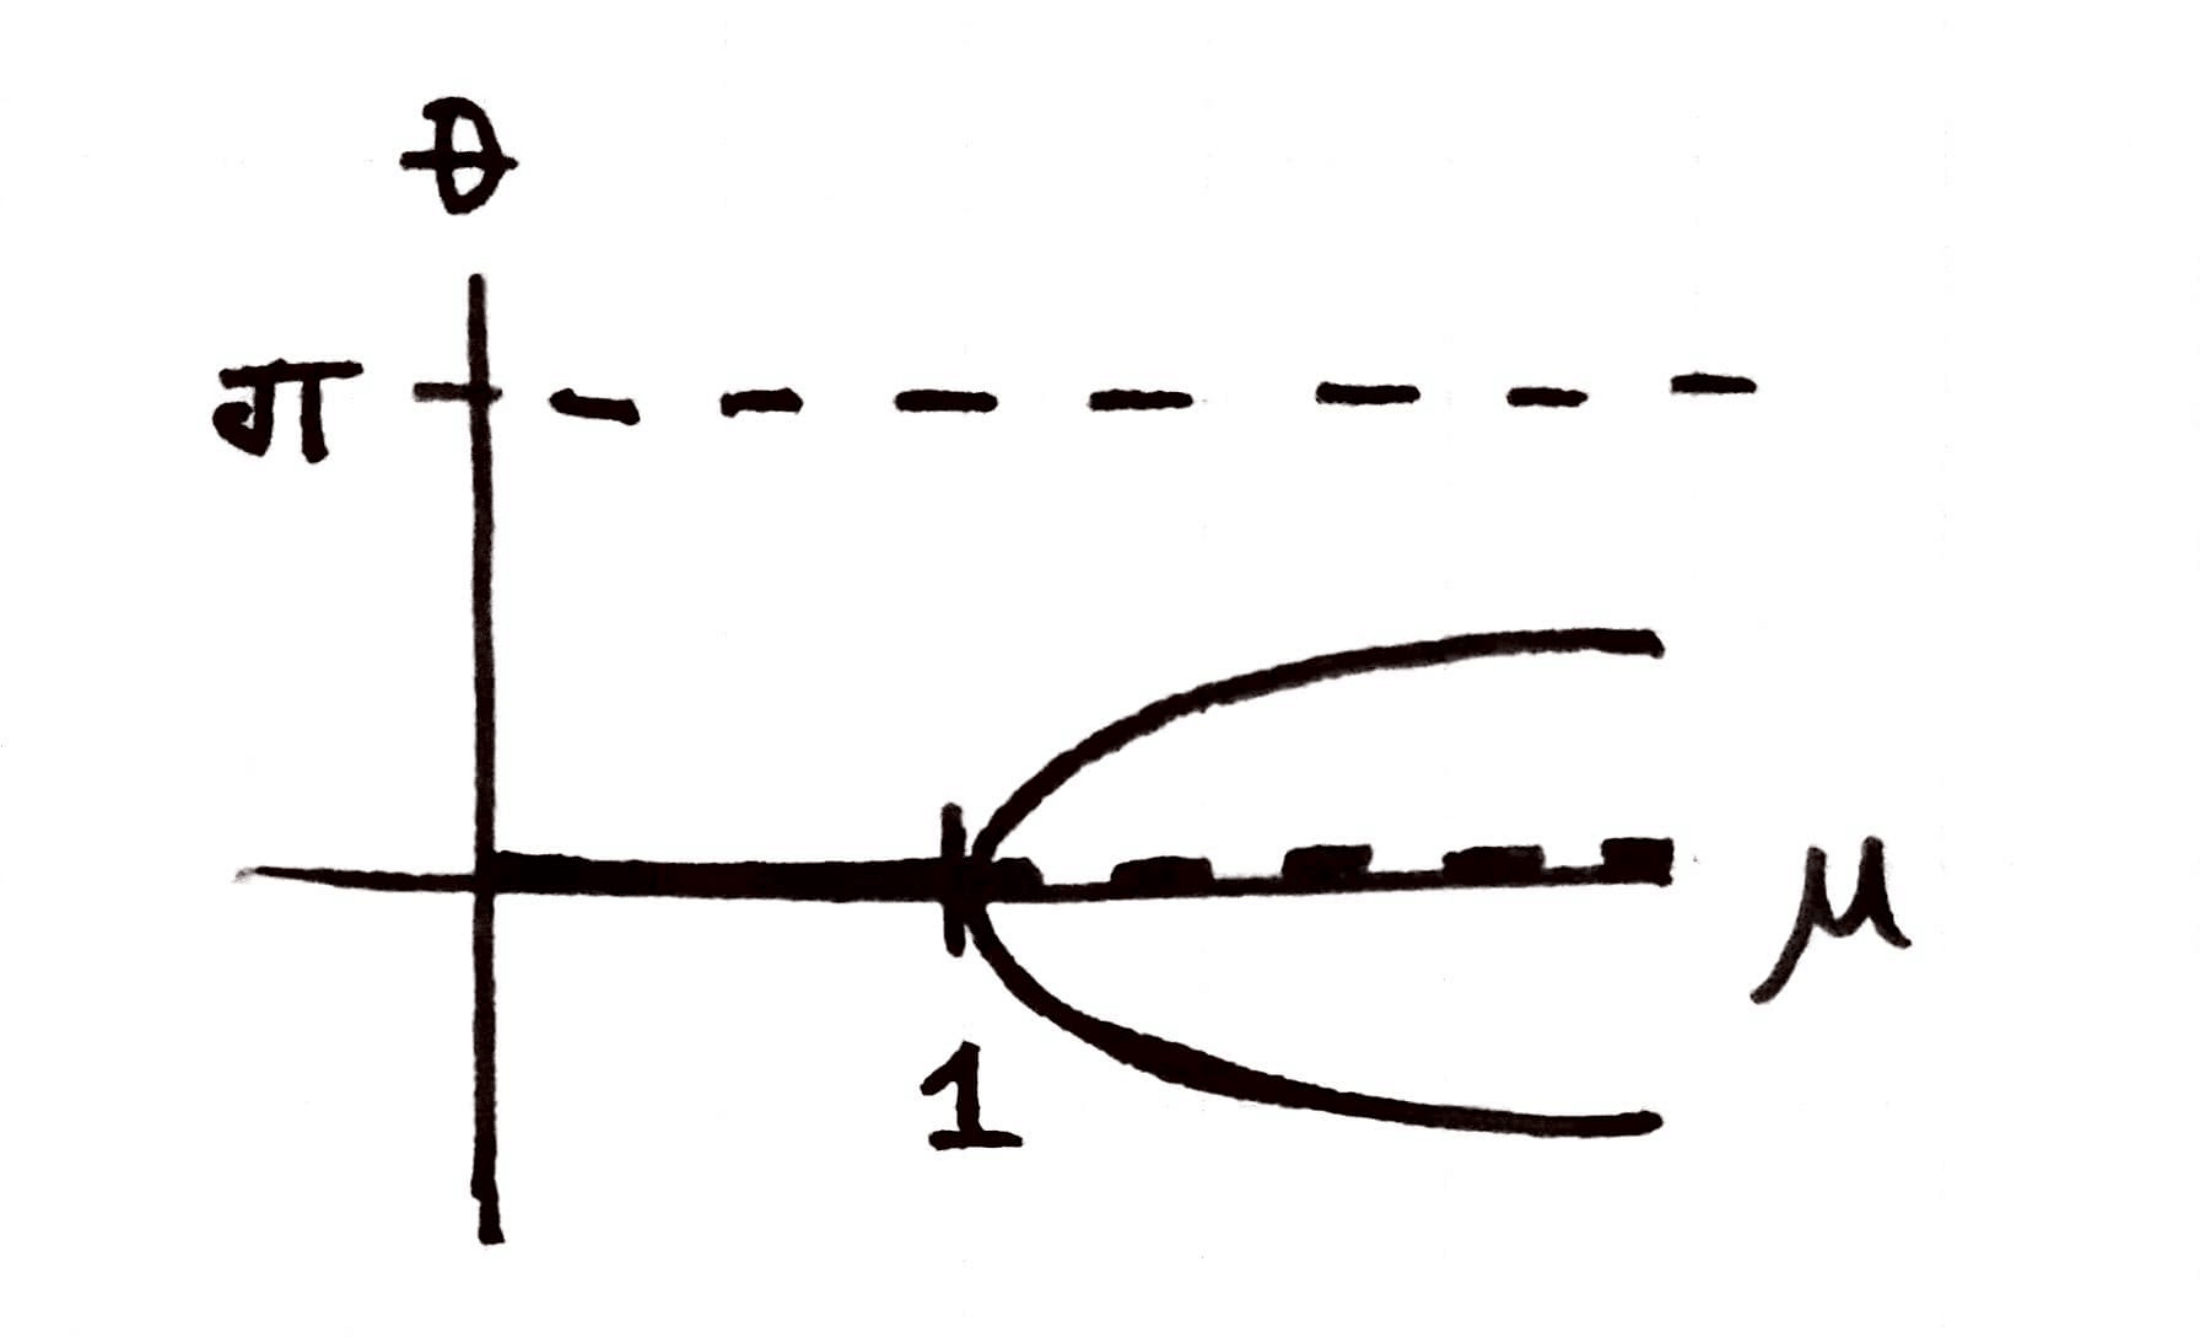
\includegraphics[height=0.3\textwidth]{img/2018F1.png}
    \end{center}
    Dashed lines indicate unstable fixed points and solid lines indicate fixed points. A supercritical pitchfork bifurcation occurs at $\mu = 1$, $\theta = 0$.
    
\end{enumerate}

\item \begin{qbox}
A solid box, with sides of unequal length, obeys Euler's equations when tossed in the
air:
\[ I\dot \omega +\omega \times I\omega = 0\]
where, for simplicity, we neglect gravity. In this equation, $I$ is the inertia tensor (defined
below) and $\omega$ is the angular velocity vector.

For a box with length $a$, height $b$, and width $c$, the inertia tensor (in Cartesian coordinates) is
\[
I = \mtx{ccc}{
\frac{m}{12}(a^2 + b^2) & 0 & 0 \\
0 & \frac{m}{12}(c^2 + b^2) & 0 \\
0 & 0 & \frac{m}{12}(a^2 + c^2)
}
\]
and the corresponding angular velocity vector is
\[
\omega = \cvec{\omega_x\\ \omega_y\\ \omega_z}.
\]
For the following, assume $a > c > b$, and $\norm{\omega} = 1$.
\begin{itemize}
    \item[(a)] Find all fixed point(s).
    \item[(b)] Use linear stability analysis to classify the fixed point(s), i.e., stable node, unstable node, center, stable spiral, unstable spiral, saddle.
\end{itemize}
\end{qbox}

\begin{enumerate}
    \item First, we must write Euler's equations as a regular system of ODEs. We begin by computing the cross product $\omega \times I\omega$. We denote each of the diagonal entries in $I$ by $I_x, I_y, I_z$.
    \begin{align*}
        \left|\begin{array}{ccc}
            \hat i & \hat j & \hat k \\
            \omega_x & \omega_y & \omega_z \\
            I_x\omega_x & I_y\omega_y & I_z\omega_z
        \end{array}\right|
        &= 
        \left|\begin{array}{cc}
            \omega_y & \omega_z \\
            I_y\omega_y & I_z\omega_z 
        \end{array}\right| \hat i
        -
        \left|\begin{array}{cc}
            \omega_x & \omega_z \\
            I_x\omega_x & I_z\omega_z 
        \end{array}\right| \hat j
        +
        \left|\begin{array}{cc}
            \omega_x & \omega_y \\
            I_x\omega_x & I_y\omega_y
        \end{array}\right| \hat k
        \\
        &=
        \omega_y\omega_z(I_z - I_y) \hat i - \omega_x\omega_z(I_z - I_x) \hat j + \omega_x\omega_y(I_y - I_x) \hat k
    \end{align*}
    
    So, our system of ODEs is
    \begin{align*}
        \begin{cases}
        \dot\omega_x = \omega_y\omega_z\cdot (I_y-I_z)/I_x = \omega_y\omega_z\cdot (b^2-a^2)/(b^2+a^2) \\
        \dot\omega_y = \omega_x\omega_z\cdot (I_z-I_x)/I_y = \omega_x\omega_z\cdot (c^2-b^2)/(c^2+b^2) \\
        \dot\omega_z = \omega_x\omega_y\cdot (I_x-I_y)/I_z = \omega_x\omega_y\cdot (a^2-c^2)/(a^2+c^2)
        \end{cases}
    \end{align*}
    The fixed points of our system (which are really fixed lines/axes) are then given by
    \[
    (x, 0, 0), (0, y, 0), \textrm{ and } (0, 0, z), \qquad \textrm{for all } x,y,z \in \R.
    \]
    
    \item We examine the Jacobian:
    \[
    J = \mtx{ccc}{
    0 & \omega_z\frac{b^2-a^2}{b^2+a^2} & \omega_y\frac{b^2-a^2}{b^2+a^2} \\
    \omega_z\frac{c^2-b^2}{c^2+b^2} & 0 & \omega_x\frac{c^2-b^2}{c^2+b^2} \\
    \omega_y\frac{a^2-c^2}{a^2+c^2} & \omega_x\frac{a^2-c^2}{a^2+c^2} & 0
    }
    \]
    First, we plug in $(x, 0, 0)$:
    \begin{align*}
        J\big\vert_{(x, 0, 0)} = \mtx{ccc}{
        0 & 0 & 0 \\
        0 & 0 & x\frac{c^2-b^2}{c^2+b^2} \\
        0 & x\frac{a^2-c^2}{a^2+c^2} & 0
        }
        \qquad
        \rightarrow
        \qquad 
        -\lambda\left(\lambda^2 - x^2\frac{c^2-b^2}{c^2+b^2}\cdot\frac{a^2-c^2}{a^2+c^2}\right) = 0
    \end{align*}
    So,
    \[
    \lambda = 0, \pm \sqrt{x^2\cdot \frac{c^2-b^2}{c^2+b^2}\cdot\frac{a^2-c^2}{a^2+c^2}}
    \]
    Since $a > c > b$, the object under our radical is positive, and so we have one zero eigenvalue, one real, positive eigenvalue, and one real, negative eigenvalue. This equilibrium is \textbf{unstable}.
    
    Next, we plug in $(0, y, 0)$:
    \begin{align*}
        J\big\vert_{(0, y, 0)} = \mtx{ccc}{
        0 & 0 & y\frac{b^2-a^2}{b^2+a^2} \\
        0 & 0 & 0 \\
        y\frac{a^2-c^2}{a^2+c^2} & 0 & 0
        }
        \qquad
        \rightarrow
        \qquad 
        -\lambda\left(\lambda^2 - y^2\frac{b^2-a^2}{b^2+a^2}\cdot\frac{a^2-c^2}{a^2+c^2}\right) = 0
    \end{align*}
    So,
    \[
    \lambda = 0, \pm\sqrt{y^2\cdot  \frac{b^2-a^2}{b^2+a^2}\cdot\frac{a^2-c^2}{a^2+c^2}}
    \]
    Since $a > c > b$, this object under the radical is negative, and so we have one zero eigenvalue and one pure imaginary pair. Because the real parts of all these eigenvalues are zero, our equilibrium is hyperbolic, and so while it's considered to be \textit{linearly} stable, we can't say anything about the true stability of this equilibrium.
    
    Finally, we plug in $(0, 0, z)$. The overall pattern will continue, and we will get
    \[
    \lambda = 0, \pm \sqrt{z^2 \cdot \frac{b^2 - a^2}{b^2 + a^2}\cdot \frac{c^2 - b^2}{c^2 + b^2} }
    \]
    Since $a > c > b$, the object under the radical is negative. So, just like above, our equilibrium is hyperbolic, and so while it's \textit{linearly} stable, we can't say anything about its true stability.
\end{enumerate}

\item
\begin{qbox}
Find a planar curve $(x, y) = (x(t), y(t))$ that minimizes the following functional:
\[
I = \int_0^1 m\left(\frac{\dot x^2 + \dot y^2}{2} - gy\right)\,dt
\]
where $m, g$ are positive constants, $(x(0), y(0)) = (0, 0)$, and $(x(1), y(1)) = (a, 0)$.

[Physically, this is a problem to find a trajectory of a projectile of mass $m$ that starts at $(0, 0)$ and hits $(a, 0)$ at time $t = 1$ under gravity.]
\end{qbox}

In the given functional, our independent variable is $t$, and we have two different functions which are dependent on $t$: $x(t), y(t)$. So, if we label our integrand as $\mathcal L$, we get two Euler-Lagrange equations to solve:
\begin{align*}
    \frac{\partial \mathcal L}{\partial x} - \frac{d}{dt}\pp{\mathcal L}{\dot x} &= 0
    \\
    \frac{\partial \mathcal L}{\partial y} - \frac{d}{dt}\pp{\mathcal L}{\dot y} &= 0
\end{align*}
Examining our first Euler-Lagrange equation, we have $\mathcal L_x = 0$ and $\mathcal L_{\dot x} = m\dot x$, so our equation becomes
\begin{align*}
    -m\ddot x &= 0 \\
    \dot x &= c_1 \\
    x &= c_1 t + c_2.
\end{align*}
Plugging in our boundary conditions $x(0) = 0$ and $x(1) = a$, we get
\[
x(t) = at.
\]
Now, examining our second Euler-Lagrange equation, we have $\mathcal L_y = -mg$ and $\mathcal L_{\dot y} = m\dot y$. So, our equation becomes
\begin{align*}
    -mg - m \ddot y &= 0 \\
    g + \ddot y &= 0 \\
    \dot y &= -gt + c_1 \\
    y &= -\frac{g}{2}t^2 + c_1t + c_2.
\end{align*}
Plugging in the boundary conditions $y(0) = y(1) = 0$, we get
\[
y = \frac{g}{2}\left(-t^2 + t\right).
\]
So, the planar curve that minimizes our functional is
\[
(x(t),y(t)) = \left(at, \frac{g}{2}\left(-t^2 + t\right)\right).
\]

\item
\begin{qbox}
Consider the Regular Sturm-Liouville Problem on the unit interval $[0, 1]$:
\[
\frac{d^2 f}{dx^2} + \lambda f = 0, \qquad f(0) = 0, \quad f(1) + f'(1) = 0.
\]
\begin{itemize}
    \item[\textbf{(a)}] Find the eigenvalues and eigenfunctions of this RSL system.
    
    [Hint: Those eigenvalues are the solutions of some transcendental (also known as \textit{secular}) equation.]
    
    \item[\textbf{(b)}] Expand the constant function 1 on $[0, 1]$ into the series of the eigenfunctions obtained in part \textbf{(a)}.
\end{itemize}
\end{qbox}

\begin{enumerate}
    \item Our RSL problem can be rewritten in the form
    \[
    \frac{d}{dx}\big[P(x) f'\big] + \big[Q(x) + \lambda R(x) \big]f = 0,
    \]
    for $P(x) = 1$, $Q(x) = 0$, and $R(x) = 1$. Since $P$ and $R$ are both positive, we may rewrite $\lambda$ in the form $\lambda = \mu^2$. So, the general solution to the above differential equation is 
    \[
    f(x) = A\cos(\mu x) + B\sin(\mu x).
    \]
    We plug in our first boundary condition, $f(0) = 0$:
    \begin{align*}
        A \cos(0) + B\sin(0) = 0
        \qquad \rightarrow \qquad
        A = 0 \qquad \rightarrow \qquad f(x) = B\sin(\mu x)
    \end{align*}
    Now we plug in the second boundary condition, $f(1) + f'(1) = 0$:
    \begin{align*}
        B\sin(\mu) + B\mu \cos(\mu) = 0
        \qquad \rightarrow \qquad
        \mu = - \tan(\mu)
    \end{align*}
    So, the eigenfunctions of this RSL system are $f_n(x) = \sin(\mu_n x)$, with eigenvalues $\mu_n$ being the solutions of the transcendental equation $\mu = -\tan\mu$.
    
    \item The goal is to find constants $c_n$ such that
    \[
    1 = \sum_{n=1}^\infty c_n\sin(\mu_n x).
    \]
    Such constants are given by:
    \begin{align*}
    c_n &= \frac{\ip{1}{\sin(\mu_n x)}}{\ip{\sin(\mu_n x)}{\sin(\mu_n x)}} \\
    &= 
    \frac{\int_0^1 \sin(\mu_n x)\,dx}{\int_0^1 \sin^2(\mu_n x)\,dx}
    \\
    &=
    \frac{(1 - \cos(\mu_n))/\mu_n}{1/2 - \sin(2\mu_n)/4\mu_n}
    \\
    &=
    \frac{4(1 - \cos(\mu_n))}{2\mu_n - \sin(2\mu_n)}
    % \\
    % &=
    % \frac{4(1 - \cos(\mu_n))}{2\mu_n - 2\sin(\mu_n)\cos(\mu_n)}
    % \\
    % &=
    % \frac{2(1 - \cos(\mu_n))}{-\tan(\mu_n) - \sin(\mu_n)\cos(\mu_n)}
    % \\
    % &=
    % \frac{2\cos(\mu_n)(1 - \cos(\mu_n))}{-\sin(\mu_n) - \sin(\mu_n)\cos^2(\mu_n)}
    % \\
    % &=
    % \frac{2\cos(\mu_n)(1 - \cos(\mu_n))}{-\sin(\mu_n)(1 + \cos^2(\mu_n)}
    % =
    % \frac{2(\cos(\mu_n) - 1)}{\tan(\mu_n) + \sin(\mu_n)\cos(\mu_n)}
    \end{align*}
\end{enumerate}

\item \begin{qbox}
The modified Bessel function $I_n(x)$ for $n$ an integer has the integral representation
\[
I_n(x) = \frac{1}{\pi} \int_0^\pi \exp\left( x\cos\theta \right)\cdot \cos(n\theta)\,d\theta.
\]
Find the leading order asymptotic expansion for $I_n(x)$ as $x \to\infty$. You may find the following integrals useful:
\[
\int_{-\infty}^\infty \exp\left( -ax^2 \right)\,dx = \sqrt{\frac{\pi}{a}},\ a > 0; 
\qquad \qquad 
\Gamma(x) = \int_0^\infty t^{x-1}e^{-t}\,dt.
\]
\end{qbox}

If we label $g(\theta) = \cos\theta$ and $f(\theta) = \cos(n\theta)$, then $e^{xg(\theta)}$ is maximized about $\theta = 0$. So, we expand $f$ and $g$ about $\theta = 0:$
\begin{align*}
    f(\theta) &\thicksim 1 \\
    g(\theta) &\thicksim 1 - \frac{1}{2}\theta^2
\end{align*}
Then, our integral is approximated by
\begin{align*}
    I_n(x) &= \frac{1}{\pi} \int_0^\pi \cos(n\theta)\cdot \exp\left( x\cos\theta \right)\,d\theta
    \\
    &\thicksim \frac{1}{\pi}\int_0^\infty \exp\left(x\left(1 - \frac{1}{2}\theta^2\right)\right)\,d\theta
    \\
    &= \frac{1}{2\pi}\int_{-\infty}^\infty \exp\left(x - \frac{x}{2}\theta^2\right)\,d\theta
    \\
    &= \frac{e^x}{2\pi}\int_{-\infty}^\infty \exp\left(- \frac{x}{2}\theta^2\right)\,d\theta
    \\
    &= \frac{e^x}{2\pi}\sqrt{\frac{\pi}{x/2}} &\textrm{(hint)}
    \\
    &=
    \frac{e^x}{\sqrt{2\pi x}}
\end{align*}

% We use Laplace's approximation. We expand $f$ and $g$ about
% \begin{align*}
%     f(\theta) &\thicksim f_0 \cdot (t - 0)^\alpha
%     & \alpha &> -1, \quad \quad\ f_0 \ne 0  \\
%     g(\theta) &\thicksim g_0 + g_1(t - 0)^{\lambda}
%     &  \lambda &> 1 + \alpha, \quad g_1 > 0
% \end{align*}
% then we will get
% \[
% I_n \thicksim \frac{1}{\pi}\left[\frac{f_0}{\lambda}\cdot \Gamma\left(\frac{1 + \alpha}{\lambda}\right)\left(\frac{1}{xg_1}\right)^{\frac{1+\alpha}{\lambda}}\right]e^{-xg_0}.
% \]
% We set
% \begin{align*}
%     f(\theta) &= \cos(n\theta) = 1 - \frac{1}{2}(n\theta)^2 + \frac{1}{4!}(n\theta)^4 - \cdots &\qquad &\rightarrow \qquad & \alpha &= 0, \quad f_0 = 1
%     \\
%     g(\theta) &= -\cos(\theta) = -1 + \frac{1}{2}\theta^2 - \frac{1}{4!}\theta^4 + \cdots &\qquad &\rightarrow \qquad & \lambda &= 2, \quad g_0 = 1, \quad g_1 = \frac{1}{2},
% \end{align*}
% and so we get
% \[
% I_n(x) \thicksim \frac{1}{\pi} \left[\frac{1}{2}\cdot\Gamma\left(\frac{1}{2}\right)\left(\frac{2}{x}\right)^{1/2}\right]e^x
% \]
% Now, we examine the $\Gamma$ term:
% \begin{align*}
% \Gamma\left(\frac{1}{2}\right) 
% &= 
% \int_0^\infty t^{-1/2}e^{-t}\,dt
% &\textrm{(hint)}
% \\
% &=
% \int_0^\infty \frac{e^{-t}}{\sqrt t}\,dt
% \\
% &=
% \int_0^\infty 2e^{-u^2}\,du 
% & \left(u = \sqrt{t}, \quad du = \frac{1}{2\sqrt t}\,dt\right)
% \\
% &=
% \int_{-\infty}^\infty e^{-u^2}\,du 
% &\textrm{(even function)}
% \\
% &= \sqrt{\pi} &\textrm{(hint; $a = 1$)}
% \end{align*}
% So, our integral approximation collapses to
% \[
% I_n \thicksim \frac{1}{\pi} \left[\frac{\sqrt \pi }{2}\left(\frac{2}{x}\right)^{1/2}\right]e^x = \frac{e^x}{\sqrt{2\pi x}}.
% \]

\item \begin{qbox}
\begin{itemize}
\vspace{-1.5em}
    \item[\textbf{(a)}]  Show that all of the solutions to
    \[ 
    \ddot u + u + \epsilon u^3 = 0,\qquad \epsilon \geq 0
    \]
    are periodic in time. [Hint: One could show that all nontrivial trajectories in the phase plane are closed curves.]
    
    \item[\textbf{(b)}] For $\epsilon = 0$, the period of the oscillation is $2\pi$. Find the leading $\epsilon$-dependent correction to the period in the limit of of small $\epsilon$ for solutions that pass through the point 
    \[
    u(t_0) = A, \qquad \dot u(t_0)(0) = 0,
    \] 
    where $t = t_0$ is some time.
\end{itemize}
\end{qbox}
\begin{enumerate}
    \item We multiply our equation by $\dot u$:
    \begin{align*}
        \ddot u \dot u + u\dot u + \epsilon u^3\dot u &= 0
        \\
        \frac{d}{dt}\left(\frac{1}{2}\dot u^2 + \frac{1}{2}u^2 + \frac{\epsilon}{4}u^4\right) &= 0
        \\
        \frac{1}{2}\dot u^2 + \frac{1}{2}u^2 + \frac{\epsilon}{4}u^4 &= C,
    \end{align*}
    where $C$ is some constant. The lefthand side of our equation is a conserved quantity, $E(u, \dot u)$, which is constant on trajectories. If we label $\dot u = v$, then we can write
    \[
    \frac{1}{2}v^2 + \frac{1}{2}u^2 + \frac{\epsilon}{4}u^4 = C,
    \]
    which describes a closed curve in $(u, v)$-space.
    
    \item We use the Poincar\'e-Lindstedt method. Let $x = \omega(\epsilon) t$, where $\omega(\epsilon) = 1 + \epsilon\omega_1$. We rewrite our equation in terms of the new variable $x:$
    \begin{align*}
        \omega^2 u'' + u + \epsilon u^3 &= 0 \\
        \left(1 + 2\epsilon\omega_1 + \epsilon^2\omega_1^2\right)u'' + u + \epsilon u^3 &= 0
    \end{align*}
    We assume $u \thicksim u_0 + \epsilon u_1$ and examine the leading-order $\Ord{1}$ equation:
    \begin{align*}
        u_0'' + u_0 = 0 \so u_0 = C\cos(x + \theta), \quad C, \theta \in \R.
    \end{align*}
    Now, we examine the $\Ord{\epsilon}$ equation:
    \begin{align*}
        2\omega_1 u_0'' + u_1'' + u_1' + u_0^3 &= 0
    \end{align*}
    We expand our $u_0$ terms:
    \begin{align*}
        2\omega_1 u_0'' + u_0^3
        &=
        -2\omega_1C\cos(x + \theta) + C^3\cos^3(x + \theta)
        \\
        &=
        -2\omega_1C\cos(x + \theta) + \frac{C^3}{4}\big[3\cos(x + \theta) + \cos(3x + 3\theta)\big]
    \end{align*}
    So, in order to eliminate secular terms, we require
    \begin{align*}
        -2\omega_1 C + \frac{3}{4}C^3 &= 0 \so
        \omega_1 = \frac{3}{8}C^2.
    \end{align*}
    Now, we use our initial conditions to solve for $C$. The condition $u'(\omega t_0) = 0$ gives
    \begin{align*}
        -C\omega\sin(\omega t_0 + \theta) = 0 \so \omega t_0 + \theta = k\pi \so \theta = k\pi - \omega t_0.
    \end{align*}
    Then, the condition $u(\omega t_0) = A$ gives
    \begin{align*}
        C \cos(\omega t_0 - \omega t_0 + k\pi) = A \so C\cdot (-1)^k = A \so C = (-1)^k A.
    \end{align*}
    Putting this all together, we get
    \begin{align*}
        u \thicksim (-1)^k A \cos\left(\omega t - \omega t_0 + k\pi \right) = A \cos\left(\omega t - \omega t_0 \right),
    \end{align*}
    which has period 
    \[
    \frac{2\pi}{\omega} = 2\pi \left(1 + \epsilon\frac{3}{8}A^2\right)^{-1}
    \]
\end{enumerate}


\end{enumerate}

\chapter*{Spring 2018}
\chaptermark{Spring 2018}
\addcontentsline{toc}{chapter}{Spring 2018}

\begin{enumerate}
\item \begin{qbox}
Consider the oscillator equation
\[
\ddot x + F(x, \dot x)\dot x  + x = 0,
\]
where $F(x, \dot x) < 0$ if $r \leq a$ and $F(x, \dot x) > 0$ if $r \geq b$, with $r^2 = x^2 + \dot x^2$ and $a < b$. Show that there is at least one closed orbit in the region $a < r < b$.
\end{qbox}

First, we convert this to a system of two first-order ODEs.
\[
\begin{cases}
\dot x = y \\
\dot y = -F(x, y)y - x
\end{cases}
\]
Next, we convert to polar coordinates. We don't need to look at the change in the $\theta$ direction, only the $r$ direction, so we compute $\dot r = x\dot x / r + y \dot y / r$:
\begin{align*}
    \dot r &= \frac{xy - F(x,y)y^2 - xy}{r}
    \\
    &=\frac{- F(x,y)y^2}{r}
\end{align*}
Since $-y^2 \leq 0$ for all $y$, we have that $\dot r \geq 0$ if $r \leq a$ and $\dot r \leq 0$ if $r \geq b$. So, flow is inward (or tangent) along the line $r = b$ and outward (or tangent) along the line $r = a$, and so we have a trapping region in $a \leq r \leq b$. By the Poincare-Bendixon theorem, there must be at least one closed orbit in the region $a < r < b$.

\item \begin{qbox}
Consider the system of ordinary differential equations
\begin{align*}
    \frac{dx}{dt} &= x(x-2y) \\
    \frac{dy}{dt} &= y(2x - y)
\end{align*}
\begin{itemize}
    \item[\textbf{(a)}] Show that $(x, y) = (0, 0)$ is the unique fixed point of the system.
    
    \item[\textbf{(b)}] Use linear stability analysis to classify the fixed point at $(x, y) = (0, 0)$. What can you conclude about the stability of $(0, 0)$ based on this analysis?
    
    \item[\textbf{(c)}] Sketch the phase portrait of the system and describe the stability of $(x, y) = (0, 0)$.
\end{itemize}
\end{qbox}

\begin{enumerate}
    \item If $\dot x = 0$, then we must have either $x = 0$ or $x = 2y$. If $\dot y = 0$, then we must have either $y = 0$ or $y = 2x$. We set our two nontrivial expressions equal to each other:
    \[
    y = 2(2y) \qquad \rightarrow \qquad -3y = 0 \qquad \rightarrow \qquad y = 0, x = 0
    \]
    So, the only fixed point in our system is $(x, y) = (0, 0)$.
    
    \item We compute the Jacobian.
    \[
    J = \mtx{cc}{2x - 2y & -2x \\ 2y & 2x -2y}
    \]
    Plugging in $(x, y) = (0, 0)$ yields the zero matrix, and so we have two zero eigenvalues. This equilibrium is hyperbolic, and so linear stability analysis tells us nothing.
    
    \item First, we draw the nullclines and figure out the direction and intensity of motion along them.
    
    The $x$-nullclines are $x = 0$ and $x = 2y$. If $x = 0$, then $\dot y = -y^2 \leq 0$, and if $x = 2y$, then $\dot y = 3y^2 \geq 0$.
    
    The $y$-nullclines are $y = 0$ and $y = 2x$. If $y = 0$, then $\dot x = x^2 \geq 0$, and if $y = 2x$, then $\dot x = -3x^2 \leq 0$.
    
    \begin{center}
    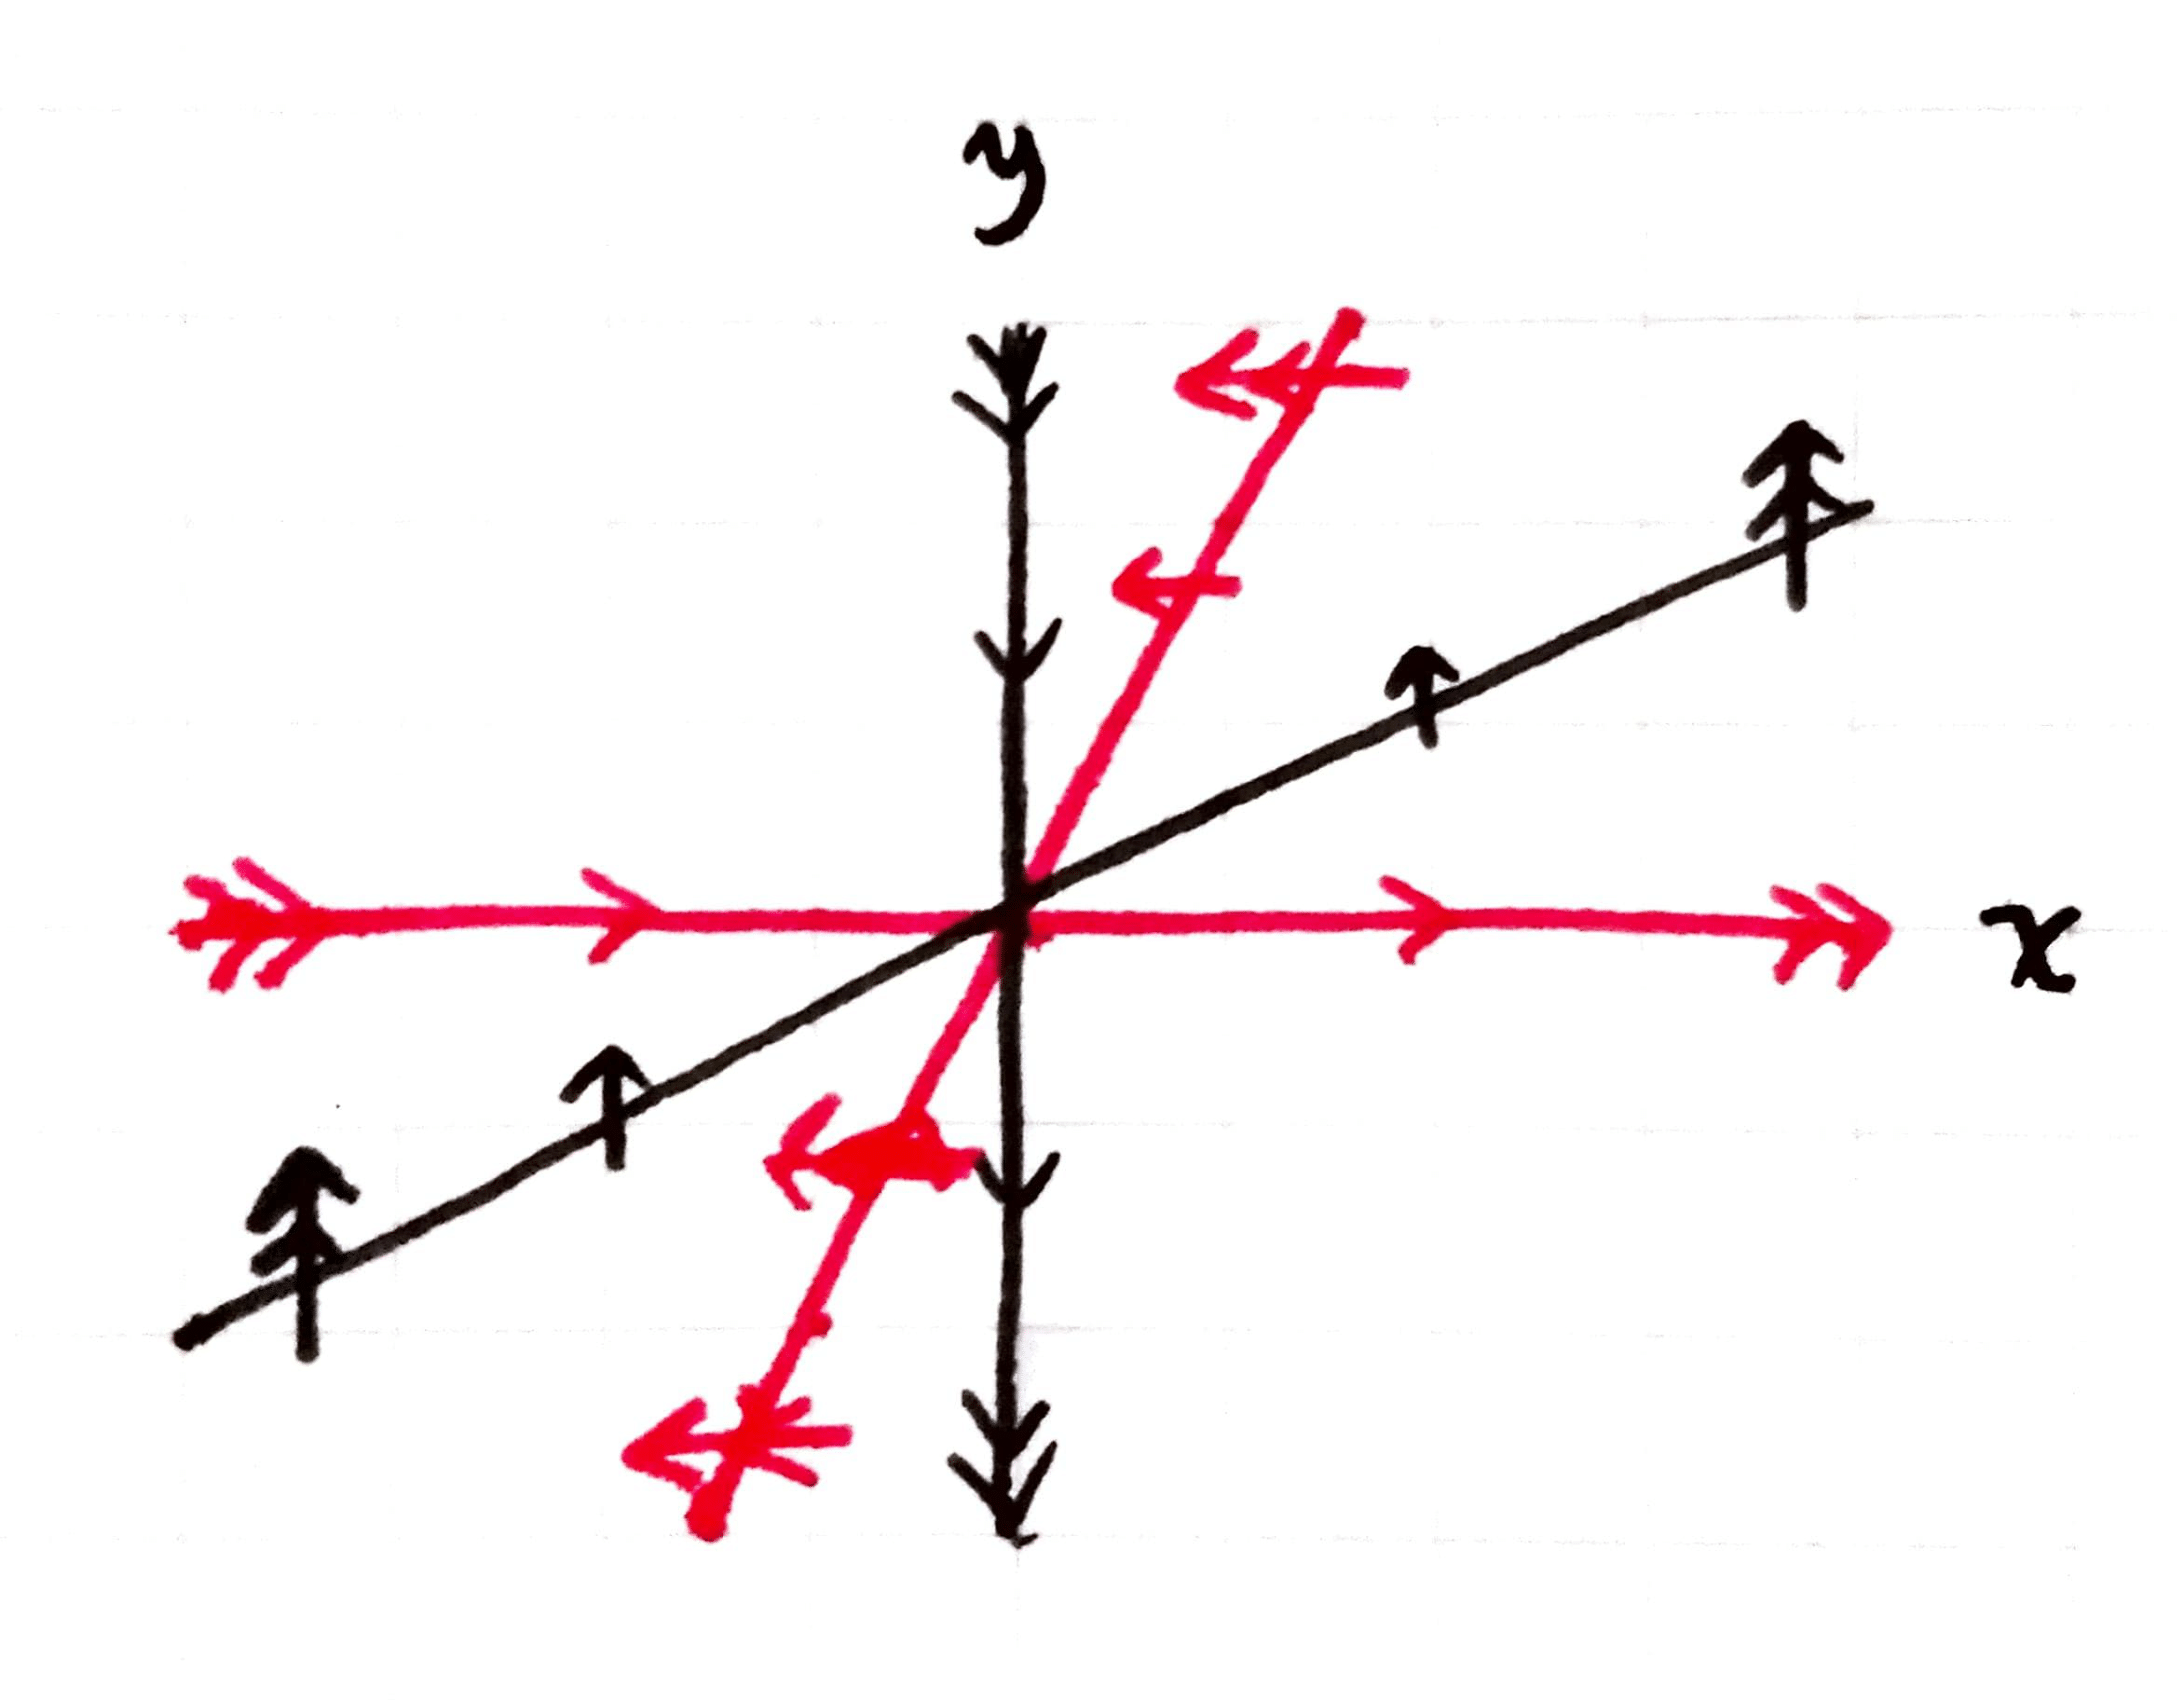
\includegraphics[height=0.3\textwidth]{img/2018S2c1.png}
    \end{center}
    Filling in the trajectories, we get the following phase portrait:
    \begin{center}
    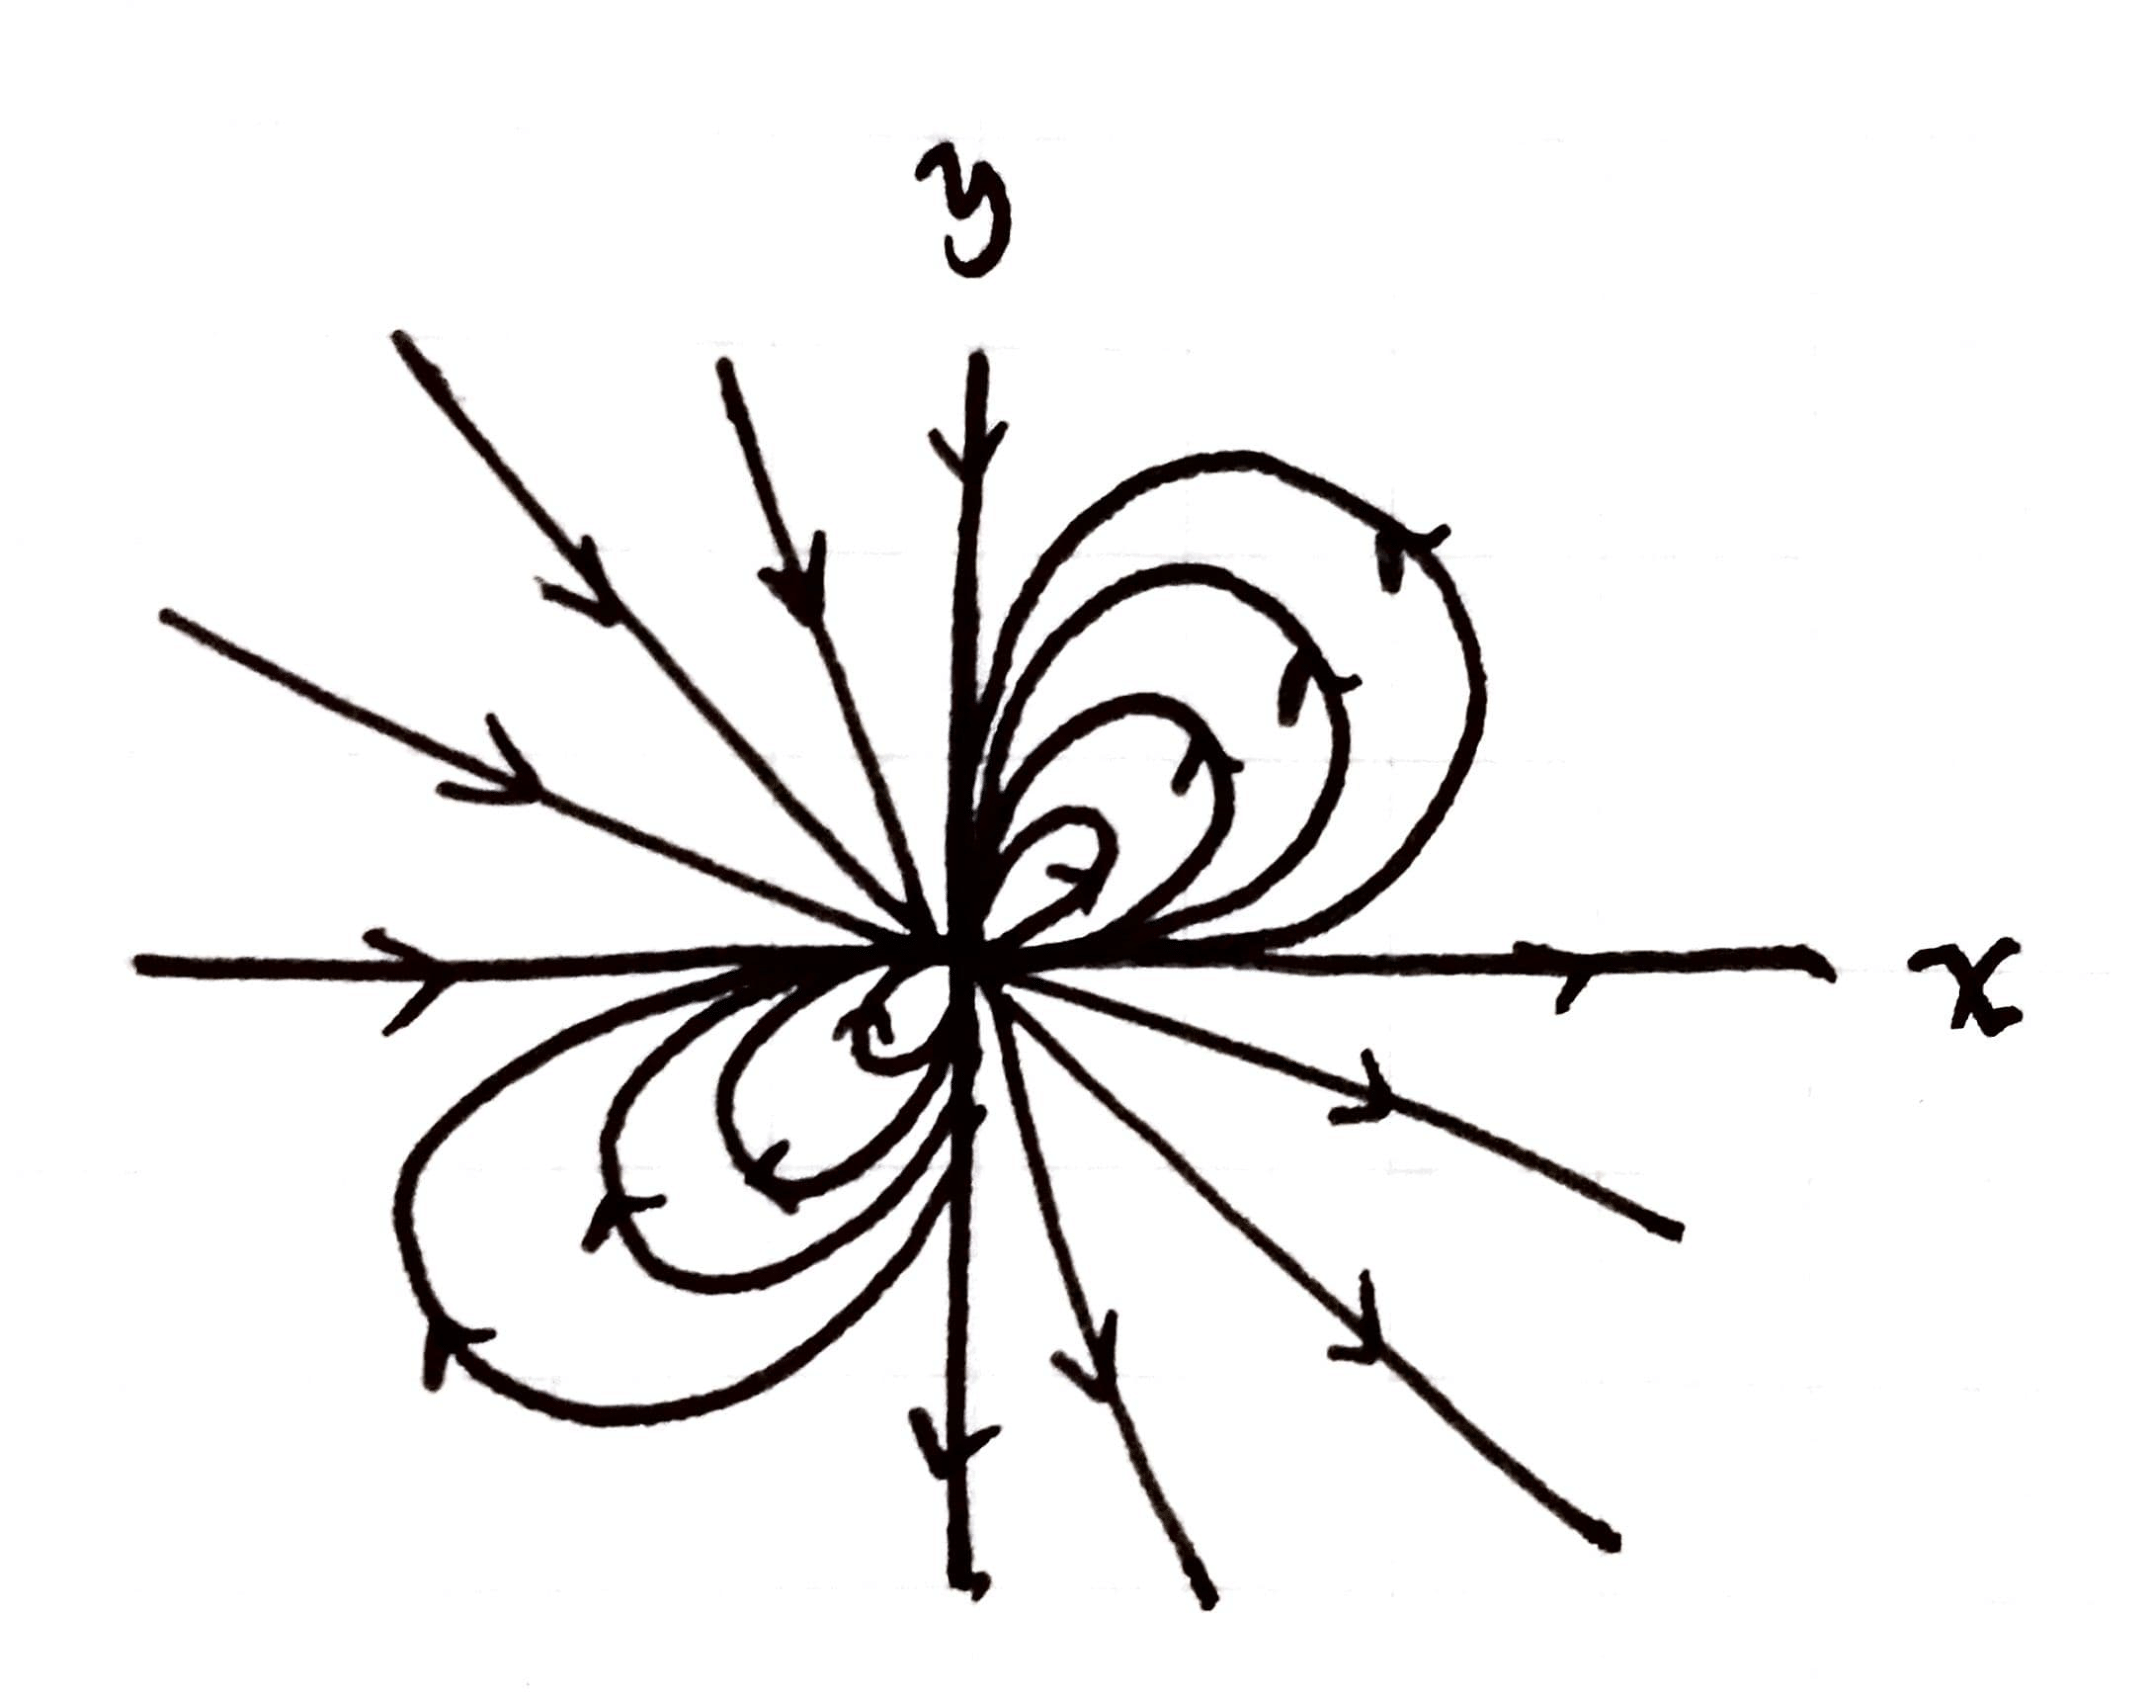
\includegraphics[height=0.3\textwidth]{img/2018S2c2.png}
    \end{center}
    The fixed point $(0, 0)$ is semi-stable: it is attracting in all regions except for in the second quadrant, where both $x \geq 0$ and $y \leq 0$.
\end{enumerate}

\item \begin{qbox}
Suppose you are given a string of length $L$. Suppose you arrange it to lie along a function, $f(x)$, where $f(0) = 0$. Of all possible potential arrangements of the string, which one maximizes the volume enclosed by it, $V$, when it is rotated about the $x$-axis?

DO NOT look for a closed form solution. Instead, leave your answer as a differential equation, boundary conditions, and a sufficient number of constraint equations to allow a clever
person with a computer to find a solution.
\end{qbox}

We set up the problem using the equation for the volume of a solid of revolution:
\[
V = \int_0^b \pi (f(x))^2\,dx, \qquad \textrm{where} \qquad \int_0^b \sqrt{1 + f'(x)^2}\,dx = L,
\]
and $f(b)$ is our free endpoint, $0 < b < L$. We use the method of Lagrange multipliers and get the integral
\[
\int_0^b \underbrace{\left(\pi f^2 + \lambda \sqrt{1 + f'^2}\right)}_{\mathcal L}\,dx,
\]
for which the Euler-Lagrange equations yield
\begin{align*}
    \frac{\partial \mathcal L}{\partial y}
    &=
    \frac{d}{dx}\frac{\partial \mathcal L}{\partial y'}
    \\
    2\pi \cdot f(x) 
    &= 
    \frac{d}{dx}\left(\frac{\lambda f'(x)}{\sqrt{1 + (f'(x))^2}}\right).
\end{align*}
The natural boundary conditions for free endpoints require
\begin{align*}
\frac{\partial \mathcal L}{\partial y'} \bigg\vert_{x = b} = 0
\so
\frac{\lambda f'(b)}{\sqrt{1 + (f'(b))^2}} = 0
\so
f'(b) = 0.
\end{align*}

\item \begin{qbox}
A plucked string, fixed at both ends, obeys the differential equation
\[
u_{tt} = c^2u_{xx} - au_t
\]
with boundary conditions $u(0,t) = u(L,t) = 0$, and initial conditions $u(x, 0) = f(x)$ and $u_t(x, 0) = 0$. In these equations, $u$ is the local displacement of the string at position $x$, and $c$ is a constant ($t$ is time). When the constant $a$ is zero, this is the wave equation; here, you will examine the effect of $a > 0$.
\begin{itemize}
    \item[\textbf{(a)}] Write the solution to the differential equation.
    
    \item[\textbf{(b)}] What happens to the solution as $t \to \infty$?
    
    \item[\textbf{(c)}] Give a possible physical interpretation of the term $au_t$.
\end{itemize}
\end{qbox}

\begin{enumerate}
    \item We use separation of variables, writing $u(x, t) = X(x)T(t)$. Then, our differential equation can be rewritten in the form
    \begin{align*}
        XT'' &= c^2 X''T - aXT'
        \\
        XT'' + aXT' &= c^2 X''T
        \\
        \frac{T''}{T} + a\frac{T'}{T} &= c^2\frac{X''}{X}
    \end{align*}
    So, for some constant $\lambda \in \R$, we have
    \[
    \frac{T''}{T} + a\frac{T'}{T} = c^2\frac{X''}{X} = \lambda.
    \]
    We examine the $X$ equation first.
    \[
    X'' - \frac{\lambda}{c^2}X = 0
    \]
    Since this equation is of the form $\left[p X'\right]' + [q + \lambda r]X = 0$ with $p$ and $r$ having opposite signs, we have $\lambda = -\mu^2 < 0$. So, we rewrite our equation accordingly:
    \[
    X'' + \left(\frac{\mu}{c}\right)^2X = 0
    \]
    Solutions have the form
    \[
    X = A\cos\left(\frac{\mu}{c}x\right) + B\sin\left(\frac{\mu}{c}x\right)
    \]
    The boundary condition $u(0, t) = 0$ is equivalently $X(0) = 0$, which yields $A = 0$. We plug in the boundary condition $u(L, t) = 0$ as $X(L) = 0$ to get
    \[
    B\sin\left(\frac{\mu}{c}L\right) = 0 \so \frac{\mu L}{c} = n\pi \so \mu_n = \frac{n\pi c}{L}, \quad n \in \N.
    \]
    So, for any $n \in \N$, we have
    \[
    X_n(x) = \sin\left(\frac{n\pi}{L}x\right).
    \]
    Now, we examine our $T$ equation.
    \begin{align*}
        T'' + aT' + \mu^2 T &= 0
    \end{align*}
    Examining the characteristic equation of this ODE, we have
    \[
    k_\pm = \frac{-a \pm \sqrt{a^2 - 4\mu^2}}{2},
    \]
    which yields solutions of the form
    \[
    T = c_1e^{k_+ t} + c_2e^{k_- t}.
    \]
    The boundary condition $u_t(x, 0) = 0$ is equivalently $T'(0) = 0$, which yields
    \begin{align*}
        c_1k_+ + c_2 k_- = 0 \so
        c_2 = -c_1\frac{k_+}{k_-},
    \end{align*}
    So for every $n \in \N$, the function $T_n$ has the form
    \[
    T_n(t) = e^{k_{+} t} - \frac{k_+}{k_-}e^{k_- t} = \exp\left(\frac{-a + \sqrt{a^2 + 4\lambda_n}}{2}\cdot t\right) - \frac{-a + \sqrt{a^2 + 4\lambda_n}}{-a - \sqrt{a^2 + 4\lambda_n}} \exp\left(\frac{-a - \sqrt{a^2 + 4\lambda_n}}{2}\cdot t\right).
    \]
    Putting this together, for any constants $c_n$, we have
    \[
    u(x, t) = \sum_{n = 1}^\infty c_nX_n(x)T_n(t) = \sum_{n = 1}^\infty c_n\sin\left(\frac{n\pi}{L}x\right)\left[e^{k_{+} t} - \frac{k_+}{k_-}e^{k_- t}\right].
    \]
    Finally, we use our last boundary condition $u(x, 0) = f(x)$, which yields our constants $c_n$.
    \[
    u(x, 0) = \sum_{n = 1}^\infty c_n\sin\left(\frac{n\pi}{L}x\right)\left(1 - \frac{k_+}{k_-}\right) = f(x)
    \]
    Since the $\sin(n\pi x/ L)$ form an orthogonal basis, we can compute the $c_n$ as follows:
    \[
    c_n\left(1 - \frac{k_+}{k_-}\right) = \frac{\ip{\sin(n\pi x/L)}{f(x)}}{\ip{\sin(n\pi x/L)}{\sin(n\pi x/L)}} = \frac{2}{L}\int_0^L \sin\left(\frac{n\pi x}{L}\right)f(x)\,dx
    \]
    So, our final solution can be expressed in the form
    \begin{align*}
    u(x, t) &= \sum_{n = 1}^\infty c_n\sin\left(\frac{n\pi}{L}x\right)\left[e^{k_{+} t} - \frac{k_+}{k_-}e^{k_- t}\right],
    \\
    c_n &= \frac{2}{L\left(1 - \frac{k_+}{k_-}\right)}\int_0^L \sin\left(\frac{n\pi x}{L}\right)f(x)\,dx,
    \\
    k_\pm &= \frac{-a \pm \sqrt{a^2 - 4n^2\pi^2c^2/L^2}}{2}.
    \end{align*}
    
    \item As $t \to \infty$, the $e^{k_+t}$ term wins out over the $e^{k_-t}$ term. This term will always have negative real part, and so our solution will decay to 0 over time.
    
    \item The $au_t$ term is a damping term, causing the solution to decay over time.
\end{enumerate}

\item \begin{qbox}
Consider projectile motion with air resistance. The (dimensional) ODE for $x(t)$, the
height of the object, is
\[
\frac{d^2x}{dt^2} = -\frac{gR^2}{(x + R)^2} - \frac{k}{x + R}\frac{dx}{dt},
\]
where $g$ is the gravitational constant, $R$ is the radius of the earth, and $k$ is a non-negative constant related to the air resistance. Suppose an object is launched from the surface $(x(0) = 0)$ at a low velocity $\frac{dx}{dt}\vert_{t = 0} = v_0$ (with $v_0$ small).
\begin{itemize}
    \item[\textbf{(a)}] Non-dimensionalize the above equation by finding appropriate re-scalings of $x$ and $t$ and define (two) small parameters in terms of your scaling choices. [HINT: Your choice of scaling should give the familiar physical problem valid when the initial velocity or displacement is much smaller than $R$ and air resistance is negligible.]
    
    \item[\textbf{(b)}] Using the non-dimensionalized equations, find the leading order asymptotic expansion for the solution. [HINT: Your expansion should be in orders of the small parameter you defined above that is \textit{independent} of the air-resistance parameter $k$.]
    
    \item[\textbf{(c)}] What equation would you need to solve to find the solution to the next highest order in the small parameter, include initial conditions, but DO NOT solve the equation.
\end{itemize}
\end{qbox}

\begin{enumerate}
    \item We define the characteristic time and length scales $x_c$ and $t_c$ so that $x = x_c\widetilde{x}$ and $t = t_c \widetilde{t}$. Then, we can rewrite our equation:
    \begin{align*}
        \frac{x_c}{t_c^2}\frac{d^2\widetilde x}{d\widetilde t^2} &= -\frac{gR^2}{(x_c\widetilde x + R)^2} - \frac{k}{x_c\widetilde x + R}\frac{x_c}{t_c}\frac{d\widetilde x}{d\widetilde t} 
        & 
        \frac{x_c}{t_c}\frac{d\widetilde x}{d\widetilde t}\bigg\vert_{\widetilde t = 0} &= v_0
        \\
        \frac{d^2\widetilde x}{d\widetilde t^2} &= -\frac{gR^2t_c^2}{x_c(x_c\widetilde x + R)^2} - \frac{kt_c}{x_c\widetilde x + R}\frac{d\widetilde x}{d\widetilde t} 
        &
        \frac{d\widetilde x}{d\widetilde t}\bigg\vert_{\widetilde t = 0} &= v_0\cdot \frac{t_c}{x_c}
    \end{align*}
    The obvious choice for $x_c$ is $x_c = R$. Our equation becomes
    \begin{align*}
        \frac{d^2\widetilde x}{d\widetilde t^2} &= -\frac{gt_c^2}{R(\widetilde x + 1)^2} - \frac{kt_c}{R\left(\widetilde x + 1\right)}\frac{d\widetilde x}{d\widetilde t} 
        &
        \frac{d\widetilde x}{d\widetilde t}\bigg\vert_{\widetilde t = 0} &= v_0\cdot \frac{t_c}{R}
    \end{align*}
    We now choose $t_c = R/v_0$. Our equation becomes
    \begin{align*}
        \frac{d^2\widetilde x}{d\widetilde t^2} &= -\frac{gR}{v_0^2}\frac{1}{(\widetilde x + 1)^2} - \frac{k}{v_0}\frac{1}{\widetilde x + 1}\frac{d\widetilde x}{d\widetilde t} 
        &
        \frac{d\widetilde x}{d\widetilde t}\bigg\vert_{\widetilde t = 0} &= 1
        \\
        \frac{v_0^2}{gR}\frac{d^2\widetilde x}{d\widetilde t^2} &= -\frac{1}{(\widetilde x + 1)^2} - \frac{kv_0}{gR}\frac{1}{\widetilde x + 1}\frac{d\widetilde x}{d\widetilde t} 
        &
        \frac{d\widetilde x}{d\widetilde t}\bigg\vert_{\widetilde t = 0} &= 1
    \end{align*}
    So, we define the two nondimensional parameters
    \[
    \epsilon = \frac{v_0^2}{gR}, \qquad \eta = \frac{kv_0}{gR}
    \]
    and so we drop the tildes in our equation and rewrite it in completely nondimensional form as
    \[
    \epsilon \ddot x + \frac{\eta}{x + 1}\dot x + \frac{1}{(x+1)^2} = 0, \qquad x(0) = 0, \quad \dot x(0) = 1.
    \]
    
    \item We assume $x \thicksim x_0 + \epsilon^\alpha x_1$. examining the leading order equation, we have
    \begin{align*}
        \frac{\eta}{x_0 + 1}\dot x_0 + \frac{1}{(x_0 + 1)^2} &= 0
        \\
        \int (x_0 + 1)\, dx_0 &= -\int \frac{1}{\eta}\,dt
        \\
        \frac{1}{2}x_0^2 + x_0 &= -\frac{1}{\eta}t + C
    \end{align*}
    Plugging in $x(0) = 0$ yields $C = 0$. So, we now have
    \begin{align*}
        \frac{1}{2}x_0^2 + x_0 + \frac{1}{\eta}t &= 0
        \\
        x_0^2 + 2x_0 + \frac{2}{\eta}t &= 0
    \end{align*}
    The quadratic formula yields
    \[
    x_0 = \frac{-2 \pm \sqrt{4 - \frac{8}{\eta} t}}{2} = -1 \pm \sqrt{1 - \frac{2}{\eta} t}
    \]
    Since our height is positive, we naturally choose the positive square root. So, our leading order asymptotic expansion is
    \[
    x \thicksim -1 + \sqrt{1 - \frac{2}{\eta} t}.
    \]
    
    \item We rewrite our equation in terms of $x_0 + \epsilon^\alpha x_1$:
    \begin{align*}
        \epsilon \ddot x + \frac{\eta}{x + 1}\dot x + \frac{1}{(x+1)^2} &= 0
        \\
        \epsilon \ddot x (x + 1)^2 + \eta(x+1)\dot x + 1 &= 0
        \\
        \epsilon(\ddot x_0 + \epsilon^\alpha x_1)(x_0^2 + 2\epsilon^\alpha x_0x_1 + \epsilon^{2\alpha}x_1^2 + 2x_0 + 2\epsilon^\alpha x_1 + 1) + \eta(x_0 + \epsilon^\alpha x_1 + 1)(\dot x_0 + \epsilon^\alpha\dot x_1) + 1 &= 0
    \end{align*}
    The clear choice for $\alpha$ is $\alpha = 1$. Then, our $\mathcal{O}(\epsilon)$ equation is
    \[
    \ddot x_0\left(x_0^2 + 2x_0 + 1\right) + \eta \left(x_1 \dot x_0 + x_0 \dot x_1 + x_1\right) = 0
    \]
    with initial conditions
    \[
    x_1(0) = 0, \qquad \dot x_1(0) = 0.
    \]
\end{enumerate}



\item \begin{qbox}
Determine the first terms in the inner and outer expansions for the following boundary value problem:
\[
\epsilon y'' - (2x + 1)y' + 2y = 0
\]
with $y(0) = 1$, $y(1) = 0$, and $\epsilon \ll 1$. Construct a first-order uniformly valid expansion for $y(x)$.
\end{qbox}

We begin with solving the first-order equation equation for our outer expansion.
\begin{align*}
    -(2x + 1)y' + 2y &= 0
    \\
    \frac{y'}{y} &= \frac{2}{2x+1}
    \\
    \ln(y) &= \ln(2x + 1) + C
    \\
    y &= C(2x + 1)
\end{align*}
Plugging in $y(0) = 1$ yields $C$ = 1, so $y = 2x + 1$, but then we cannot fit our other condition, $y(1) = 0$. So, we suspect a boundary layer at $x = 1$. For now, we have $y_{out} \thicksim 2x + 1$.

To solve for our inner solution, we rescale $x$, assuming $\alpha  > 0$:
\[
\hat x = \frac{x - 1}{\epsilon^\alpha} \so \dd{y}{x} = \dd{y}{\hat x}\dd{\hat x}{x} = \epsilon^{-\alpha}\frac{dy}{d\hat x}
\]
So, we now write $y'$ as $dy/d\hat x$, and our boundary value problem becomes
\begin{align*}
\epsilon^{1 - 2\alpha}y'' - \left(2\epsilon^\alpha \hat x + 3\right)\epsilon^{-\alpha}y' + 2y 
&= 
0
\\
\undernum{\epsilon^{1 - 2\alpha}y''}{1} - \undernum{2\hat x y'}{2} - \undernum{3\epsilon^{-\alpha}y'}{3} + \undernum{2y}{2} 
&= 
0
\end{align*}
We match terms.
\begin{alignat*}{5}
    (1) &\thicksim (2): &\  1 - 2\alpha &= 0 &\so \alpha &= 1/2 &\qquad \rightarrow &\qquad (1), (2): \mathcal{O}(1), \quad (3): \mathcal{O}(\epsilon^{-1/2}) \quad (\times)
    \\
    (1) &\thicksim (3): &\  1 - 2\alpha &= -\alpha &\so \alpha &= 1 &\qquad \rightarrow &\qquad (1), (3): \mathcal{O}(\epsilon^{-1}), \quad (2): \mathcal{O}(1) \quad (\checkmark)
    \\
    (2) &\thicksim (3): &\  \alpha &= 0 \qquad (\times)
\end{alignat*}
The clear choice is $\alpha = 1$. So, our equation may be rewritten as
\[
\epsilon^{-1}\left(y'' - 3y'\right) - 2\hat x y' + 2y = 0.
\]
Our leading-order expression gives
\begin{align*}
    y'' - 3y' &= 0
    \\
    y'' &= 3y'\\
    y' &= c_1 e^{3\hat x}
    \\
    y &= c_1 e^{3\hat x} + c_2
\end{align*}
Rewriting in terms of $x$, we get
\[
y_{in} \thicksim c_1\exp\left(\frac{3(x-1)}{\epsilon}\right) + c_2.
\]
We solve for our previously unmet boundary condition: $y(1) = 0$:
\[
0 = c_1 + c_2 \so c_2 = - c_1
\]
Therefore, we have
\[
y_{in} \thicksim C\left(\exp\left(\frac{3(x-1)}{\epsilon}\right) - 1\right).
\]
Now, we match.
\begin{align*}
\lim_{x \to 1} y_{out} &= \lim_{x \to 1} 2x + 1 = 3
\\
\lim_{x \to -\infty} y_{in} &= \lim_{x \to -\infty} C\left(\exp\left(\frac{3(x-1)}{\epsilon}\right) - 1\right) = -C
\end{align*}
So, we have $C = -3$, and $y_{overlap} = 3$. Putting this together, we have
\begin{align*}
    y &\thicksim 
    y_{out} + y_{in} - y_{overlap} 
    \\
    &= 
    2x + 1 - 3\exp\left(\frac{3(x-1)}{\epsilon}\right) + 3 - 3 \\
    &= 
    2x + 1 - 3\exp\left(\frac{3(x-1)}{\epsilon}\right).
\end{align*}
\end{enumerate}

\chapter*{Fall 2017}
\chaptermark{Fall 2017}
\addcontentsline{toc}{chapter}{Fall 2017}
\begin{enumerate}
\item 
\begin{qbox}
Consider the system of ordinary differential equations
\begin{align*}
    \frac{dx}{dt} &= x(1-x^2-y^2) - 2y(1+x)
    \\
    \frac{dy}{dt} &= y(1-x^2-y^2) + 2x(1+x)
\end{align*}
\begin{itemize}
    \item[\textbf{(a)}] Use the function $V(x, y) = (1 - x^2 - y^2)^2$ like a Lyapunov function to prove the existence of an asymptotically stable closed orbit.
    \item[\textbf{(b)}] Is the asymptotically stable closed orbit a limit cycle? Briefly justify your answer
\end{itemize}
\end{qbox}
\begin{enumerate}
    \item We examine the time derivative of $V$:
    \begin{align*}
        \frac{dV}{dt} &= \frac{dV}{dx}\dd{x}{t} + \dd{V}{y} \dd{y}{t}
        \\
        &= 2(1-x^2 - y^2)(-2x)\dot x + 2(1-x^2-y^2)(-2y)\dot y
        \\
        &=
        -4\left(1-x^2-y^2\right)(x\dot x + y \dot y)
        \\
        &=
        -4\left(1-x^2-y^2\right)\left(x^2(1-x^2-y^2) - 2xy(1+x) + y^2(1-x^2-y^2) + 2xy(1+x)\right)
        \\
        &=
        -4\left(1-x^2-y^2\right)^2\left(x^2+y^2\right)
        \\
        &\leq 0
    \end{align*}
    So, we have that $dV/dt \leq 0$ everywhere, and $dV/dt = 0$ only when $x^2 + y^2 = 0$ (which is at the fixed point $(x, y) = 0$) and at $x^2 + y^2 = 1$. Moreover, $V(x, y) \geq 0$ everywhere, with $V(x, y) = 0$ exactly when $x^2 + y^2 = 1$. Therefore, we have an asymptotically stable closed orbit at $x^2 + y^2 = 1$.
    
    \item Yes, it is a limit cycle. Because it's attracting, nearby orbits spiral into it, and so it's isolated.
\end{enumerate}

\item \begin{qbox}
Consider the system of ordinary differential equations
\begin{align*}
    \frac{dx}{dt} &= x^2 - y
    \\
    \frac{dy}{dt} &= 2\alpha x - y - \beta
\end{align*}
with the parameters $\alpha, \beta > 0$.
\begin{itemize}
    \item[\textbf{(a)}] Find and classify all bifurcations of steady states that occur in the system. (That is, identify all saddle-node, pitchfork, transcritical, and/or Hopf bifurcations. For any pitchfork or Hopf bifurcations, you do NOT have to determine whether they are super- or sub-critical).
    
    \item[\textbf{(b)}] Plot the stability diagram (i.e., two-parameter bifurcation diagram) for the system in the $\alpha,\beta$-plane. A codimension-2 bifurcation called a Taken-Bogdonov bifurcation occurs at $\alpha = 1/2,\ \beta = 1/4$. Very briefly describe what happens at this point.
\end{itemize}
\end{qbox}
\begin{enumerate}
    \item First, we find our steady states. Clearly $\dot x = 0$ when $y = x^2$. For $\dot y = 0$, we have
    \[
    2\alpha x - y - \beta = 0 \so x = \frac{2\alpha \pm \sqrt{4\alpha^2-4\beta}}{2} = \alpha \pm \sqrt{\alpha^2 - \beta}.
    \]
    So, in the most general case, we have two fixed points:
    \[
    (x, y) =
    \left(\alpha + \sqrt{\alpha^2 - \beta},\ \left(\alpha + \sqrt{\alpha^2 - \beta}\right)^2\right),\ 
    \left(\alpha - \sqrt{\alpha^2 - \beta},\ \left(\alpha - \sqrt{\alpha^2 - \beta}\right)^2\right)
    \]
    Based on the values under the radicals, we get the following cases:
    \begin{align*}
        \alpha^2 < \beta &: \textrm{0 fixed points}
        \\
        \alpha^2 = \beta &: \textrm{1 fixed point}: (x, y) = (\alpha, \alpha^2)
        \\
        \alpha^2 > \beta &: \textrm{2 fixed points}
    \end{align*}
    So, clearly a saddle-node bifurcation occurs at $\alpha^2 = \beta$. Since there are no other situations where fixed points are created or destroyed, we know that there won't be any pitchfork or transcritical bifurcations, but this still leaves the case where there may be a Hopf bifurcation.
    
    To check for a hopf bifurcation, we need to see if at any point the real part of the eigenvalues of one of our fixed points passes through zero, resulting in a pure imaginary eigenvalue pair. 
    
    We examine the Jacobian of our system in the general case:
    \begin{align*}
    J = \mtx{cc}{2x & -1 \\ 2\alpha & -1} \so (2x - \lambda)(-1-\lambda)+2\alpha &= 0
    \\
    \lambda^2 + (1 - 2x)\lambda + 2(\alpha - x) &= 0
    \end{align*}
    This results in the following eigenvalues:
    \begin{align*}
        \lambda &= \frac{-(1-2x) \pm \sqrt{(1-2x)^2 - 8(\alpha - x)}}{2}
    \end{align*}
    Two things must happen to get a Hopf bifurcation here: we must have $1 - 2x = 0$, and the object under our radical must be negative.
    
    Since we require $1 - 2x = 0$, we have $x = 1/2$, which would require $\alpha \pm \sqrt{\alpha^2 - \beta} = 1/2$. So,
    \begin{align*}
        \pm \sqrt{\alpha^2 - \beta} &= \frac{1}{2} - \alpha
        \\
        \alpha^2 - \beta &= \left(\frac{1}{2} - \alpha\right)^2
        \\
        \alpha^2 - \beta &= \frac{1}{4} - \alpha + \alpha^2
        \\
        \beta &= \alpha - \frac{1}{4}.
    \end{align*}
    Now, our other requirement is that $(1-2x)^2 - 8(\alpha - x) < 0$. Note from earlier that $1-2x = 0$, and so this collapses to the requirement $\alpha > x$. Moreover, $1 - 2x = 0$ is equivalent to $x = 1/2$, and so this requirement is truly $\alpha > 1/2$.
    
    In total, we expect a Hopf bifurcation when $\alpha > 1/2$ and $\beta = \alpha - 1/4$. We need a fixed point to exist for it to undergo such a bifurcation, though, so we also require $\alpha^2 \geq \beta$. We briefly check that such a point exists:
    \begin{align*}
        \alpha^2 \geq \alpha - \frac 1 4 \\
        \alpha^2 - \alpha + \frac 1 4 &\geq 0 \\
        \left(\alpha - \frac{1}{2}\right)^2 \geq 0
    \end{align*}
    Yes, there are indeed valid $\alpha > 1/2$ such that this will happen.
    
    \item At the point $\alpha = 1/2,\ \beta = 1/4$, two bifurcations collide: both a saddle-node bifurcation and a Hopf bifurcation. Depending on which direction we move across this bifurcation point in, we can either move between no fixed points and two fixed points, or two fixed points can temporarily collide into one and then re-separate, or we could change stability.
    
    \begin{center}
    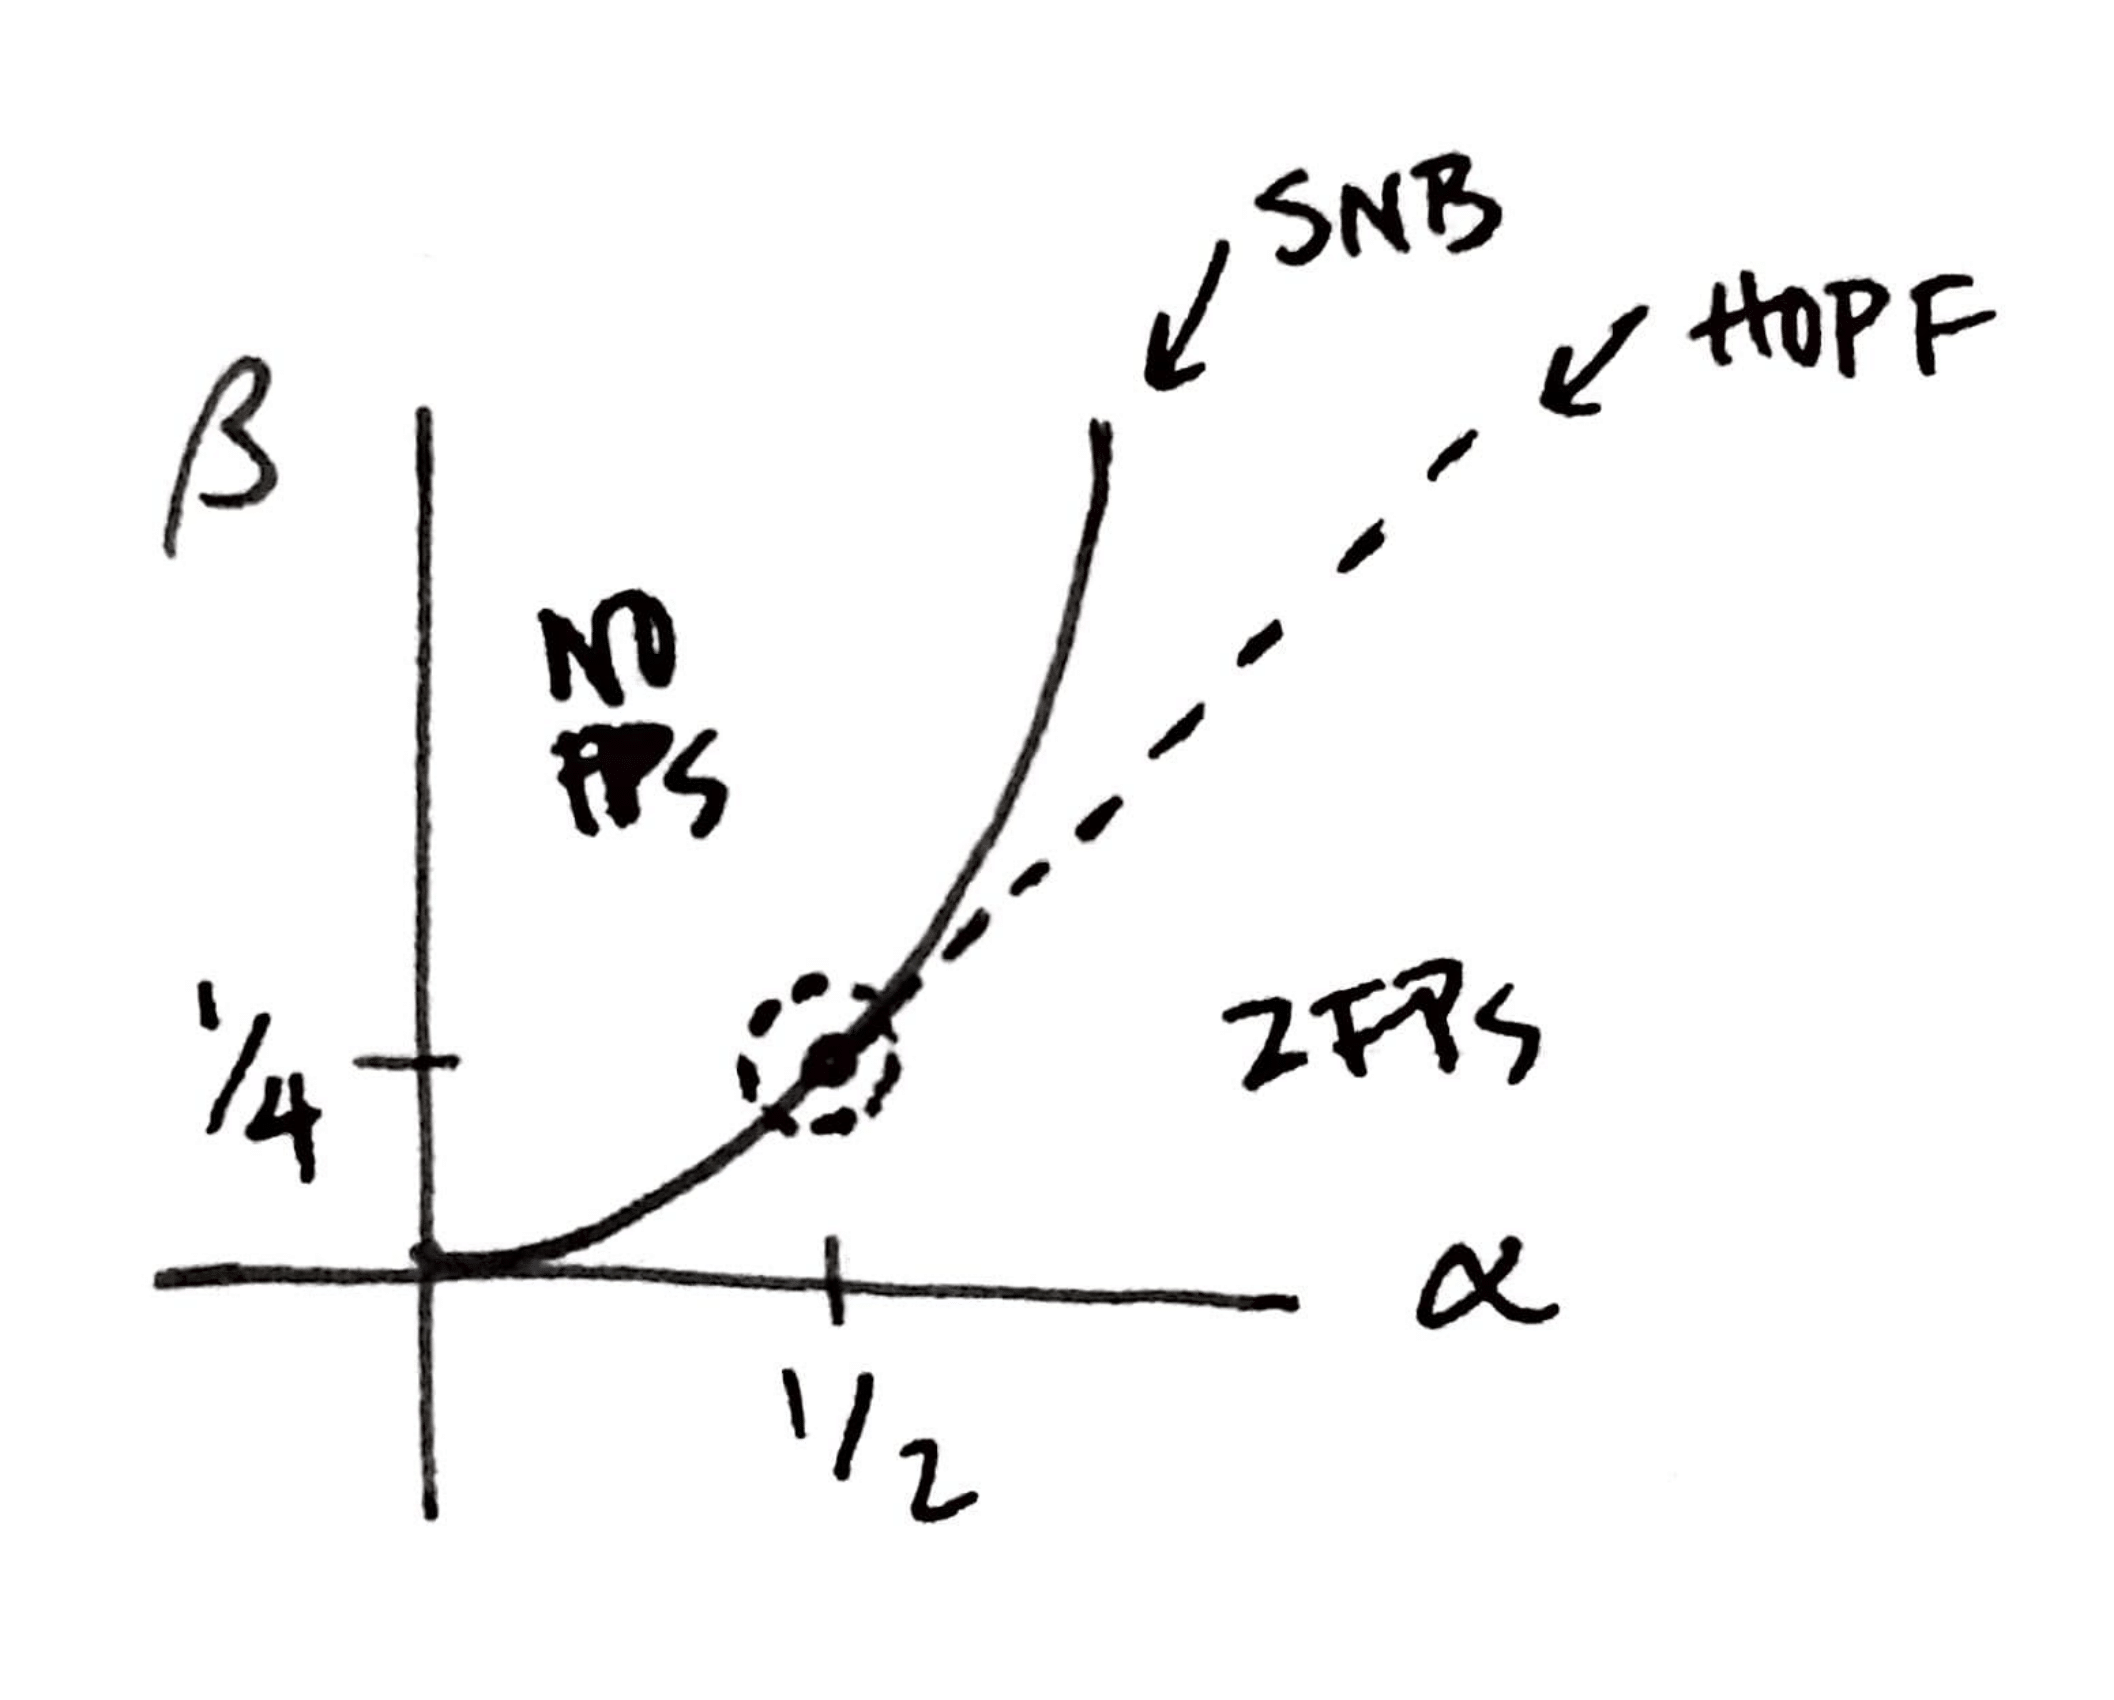
\includegraphics[height=0.3\textwidth]{img/2017F2.png}
    \end{center}
\end{enumerate}

\item \begin{qbox}
Suppose you are given a string of length $L$. Of all possible potential arrangements of the string, which one maximizes the area enclosed by it, $A$?

Assume (1) that the shape of the string is symmetric; and (2) that half of the string (of length $L/2$) can be described by the function $f(x)$, defined for $a \leq x \leq b$, such that $\int_a^b f(x)\,dx = A/2$.
\end{qbox}

Without loss of generality, we allow the $x$-axis to be the axis of symmetry for our string, and we position it so that its leftmost point is at the origin. In this way, we have $f(x) \geq 0$ for $0 < x < b$, where $f(0) = f(b) = 0$. 

Intuitively, we expect any shape with a fixed perimeter which maximizes the area in encloses to be a circle. So, we expect $f$ to be a semicircle with arc length $L/2$, that is, to be of the form $(x - r)^2 + f^2 = r^2$, where $\pi r = L/2$. On geometric intuition alone, we expect our answer to be
\[
f(x) = \sqrt{\left(\frac{L}{2\pi}\right)^2 - \left(x - \frac{L}{2\pi}\right)^2}.
\]
We now prove this result using calculus of variations. Our goal is to maximize the integral
\[
\mathcal{L} = \int_0^b f(x)\,dx = \frac{A}{2}
\]
subject to the constraint
\[
\int_0^b\sqrt{1 + \left[f'(x)\right]^2}\,dx = \frac{L}{2}.
\]
We define
\[
h = f + \lambda \sqrt{1 + \left[f'(x)\right]^2}.
\]
Then, the Euler-Lagrange equation gives
\begin{align*}
\pp{h}{f} &= \frac{d}{dx}\left[\pp{h}{f'}\right]
\\
1 &= \frac{d}{dx}\left[\frac{\lambda f'}{\sqrt{1 + f'^2}}\right]
\\
x + c &= \frac{\lambda f'}{\sqrt{1 + f'^2}} &\textrm{(for $c$ some constant)}
\\
(x + c)\sqrt{1 + f'^2} &= \lambda f'
\\
(x + c)^2\left(1 + f'^2\right) &= \lambda^2 f'^2
\\
(x+c)^2 &= \left(\lambda^2 - (x+c)^2\right)f'^2
\\
f'^2 &= \frac{(x+c)^2}{\lambda^2 - (x+c)^2}
\\
f' &= \pm \frac{x+c}{\sqrt{\lambda^2 - (x+c)^2}}
\end{align*}
Since we expect $f'(0) \geq 0$, we take only the positive version:
\[
f' = \sgn{c}\cdot \frac{x+c}{\sqrt{\lambda^2 - (x+c)^2}}
\]
(This isn't exactly correct --- if $c = 0$, then we'll consider $\sgn(c) = 1$, but it's more concise for now). We integrate $f$.
\begin{align*}
    f(x) &= \sgn(c) \int\frac{x+c}{\sqrt{\lambda^2 - (x+c)^2}}\,dx\\
    &=
    \sgn(c) \int \frac{u}{\sqrt{\lambda^2 - u^2}}\,du
    \\
    &=
    - \frac{1}{2}\sgn(c) \int \frac{dw}{\sqrt{w}} &\left(w = \lambda^2 - u^2,\ dw = -2u\,du\right)
    \\
    &=
    - \sgn(c)\sqrt{w} + d
    \\
    &=
    - \sgn(c)\sqrt{\lambda^2 - (x+c)^2} + d
\end{align*}
Since $f(0) = 0$, this becomes
\[
f(x) = -\sgn(c) \sqrt{\lambda^2 - (x+c)^2} + \sqrt{\lambda^2 - c^2}
\]
We'll assume that $f$ is smooth, since it represents a real object. Since $f$ is symmetric, we will expect $\lim_{x \to 0}f'(x) = \infty$, and so we expect
\[
\sqrt{\lambda^2 - c^2} = 0 \so c = \pm \lambda,
\]
so, we collapse $f$ to 
\[
f(x) = -\sgn(c) \sqrt{\lambda^2 - (x+c)^2}.
\]
Without loss of generality, we assume $\lambda > 0$. Moreover, we have that $f(b) = 0$, which gives
\begin{align*}
-\sgn(c)\sqrt{\lambda^2 - (b + c)^2} &= 0
\\
\lambda^2 &= (b + c)^2 = b^2 + 2bc + \lambda^2
\\
b(b + 2c) &= 0
\\
c &= -\frac{1}{2}b.
\end{align*}
Since $b > 0$, we therefore have $c < 0$, and so
\[
c = -\lambda \quad\textrm{and}\quad b = 2\lambda.
\]
Thus, 
\[
f(x) = \sqrt{\lambda^2 - (x-\lambda)^2}.
\]
Finally, we plug $f$ into our integral constraint to solve for $\lambda$.
\begin{align*}
\frac{L}{2} &= 
\int_0^b \sqrt{1 + \left[f'(x)\right]^2}\,dx
\\
&=
\int_0^{2 \lambda} \sqrt{1 + \frac{(x - \lambda)^2}{\lambda^2 - (x - \lambda)^2}}\,dx
\\
&=
\int_0^{2 \lambda} \sqrt{\frac{\lambda^2}{\lambda^2 - (x - \lambda)^2}}\,dx
\\
&=
\lambda\int_0^{2 \lambda} \frac{dx}{\sqrt{\lambda^2 - (x - \lambda)^2}}
\\
&=
\lambda\int_{-\lambda}^{\lambda} \frac{du}{\sqrt{\lambda^2 - u^2}}
&
(u = x - \lambda)
\\
&=
\lambda\int_{-\pi/2}^{\pi/2} \frac{\lambda\cos w }{\sqrt{\lambda^2 - \lambda^2\sin^2 w}}\,dw
&
(u = \lambda\sin w \rightarrow w = \sin^{-1}(u/\lambda))
\\
&=
\lambda\int_{-\pi/2}^{\pi/2} \frac{\lambda\cos w }{\sqrt{\lambda^2\cos^2 w}}\,dw
\\
&=
\lambda\int_{-\pi/2}^{\pi/2}\,dw
\\
&=
\lambda\pi
\end{align*}
So, we end up with $\lambda = L/ 2\pi$. Our final function is thus
\[
f(x) = \sqrt{\left(\frac{L}{2\pi}\right)^2 - \left(x - \frac{L}{2\pi}\right)^2}.
\]

\item \begin{qbox}
A uniform, isotropic, linear-elastic beam of length $L$, subject to small transverse displacements has action $\mathcal L$,
\[
\mathcal L = \int_0^L \left(-a^2 \frac{1}{2}u_x^2 + \frac{1}{2}u_t^2\right)\,dx,
\]
where $u$ is the local displacement at position $x$ along the beam, and $a$ is a constant ($t$ is time, and the equation is non-dimensionalized).
\begin{itemize}
    \item[\textbf{(a)}] Derive a partial differential equation for the function, $u(x,t)$, that minimizes the action $\mathcal L$.
    \item [\textbf{(b)}] Suppose that the beam is fixed at one end ($u(0,t) = 0$), and free at the other ($u_x(L,t) = 0$). Solve the PDE you derived in part (a) for arbitrary initial displacement ($u(x, 0) = f (x)$) and zero initial velocity ($u_t(x, 0) = 0$).
    
    \item[\textbf{(c)}] Find the solution for the case where the beam is struck at the free end ($u_t(x, 0) = b\cdot \delta (x - L)$, where $b$ is an arbitrary positive constant, and $\delta(x)$ is the Dirac delta function). 
    
    Note, it may be useful to recall the property
    \[
    \int_a^b f(x)\delta(x - c)\,dx = f(c) \qquad \textrm{if}\quad a < c < b.
    \]
\end{itemize}
\end{qbox}
\begin{enumerate}
\item We use the Euler-Lagrange equation:
\begin{align*}
    \pp{f}{u} - \frac{d}{dx}\left[\pp{f}{u_x}\right] - \frac{d}{dt}\left[\pp{f}{u_t}\right] &= 0
    \\
    -\frac{d}{dx}\left[-a^2u_x\right] - \frac{d}{dt}\big[u_t\big]
    &= 0
    \\
    a^2 u_{xx} - u_{tt} &= 0.
\end{align*}
    
\item We assume $u(x, t)$ has the form $u(x, t) = X(x)T(t)$. Then,
\begin{align*}
    a^2 X''(x)T(t) &= X(x)T''(t) \\
    a^2\frac{X''}{X} &= \frac{T''}{T} = \lambda,
\end{align*}
where $\lambda$ is some constant. Our boundary conditions become $X(0) = 0$, $X'(L) = 0$, $T'(0) = 0$, and $X(x)T(0) = f(x)$. First, we show $\lambda \leq 0:$
\begin{align*}
    a^2X'' &= \lambda X \\
    a^2X''X &= \lambda X^2 \\
    a^2X'X\bigg\vert_{0}^L - a^2 \int \left(X'\right)^2\,dx &= \lambda \int X^2\,dx
\end{align*}
The boundary terms vanish, and so we get
\[
- a^2 \int \left(X'\right)^2\,dx = \lambda \int X^2\,dx.
\]
Since both integrals are nonnegative, we must have $\lambda \leq 0$. So, we label $\lambda = -\mu^2$. Now, we go back to solve for $X(x)$.
\begin{align*}
    a^2 X'' &= -\mu^2 X
    \\
    X(x) &= A\sin\left(\frac{\mu}{a}x\right) + B\cos\left(\frac{\mu}{a}x\right)
\end{align*}
The boundary condition $X(0) = 0$ gives $B = 0$, and so
\[
X(x) = A\sin\left(\frac{\mu}{a}x\right) \so X'(x) = A\cdot \frac{\mu}{a}\cos\left(\frac{\mu}{a}x\right)
\]
The boundary condition $X'(L) = 0$ gives us the following:
\begin{align*}
    A\cdot \frac{\mu}{a}\cos\left(\frac{\mu}{a}L\right) &= 0
    \\
    \frac{\mu L}{a} &= \frac{\pi}{2} + k\pi
    \\
    \mu_k &= \frac{a \pi}{L}\left(k + \frac{1}{2}\right), \qquad k \in \N
\end{align*}
So,
\[
X_k(x) = \sin\left(\frac{\mu_k}{a}x\right) = \sin\left(\frac{\pi }{L}\left(k + \frac{1}{2}\right)x\right), \qquad k \in \N.
\]
Next, we solve for $T$.
\begin{align*}
    T'' = -\mu^2 T \so T(t) &= A\sin(\mu t) + B\cos(\mu t)
    \\
    T'(t) &= A\cos(\mu t) - B\sin(\mu t)
\end{align*}
The initial condition $T'(0) = 0$ gives $A = 0$, and so 
\[
T = B\cos(\mu t).
\]
So, $u(x, t)$ has the form
\begin{align*}
u(x, t) &= \sum_{k \in \N} C_k X_k(x)T_k(x)
\\
&= \sum_{k \in \N} C_k \sin\left(\frac{\mu_k}{a}x\right)\cos(\mu_k t),
\end{align*}
where $\mu_k$ is defined as above. To find $C_k$, we utilize our last boundary condition: $u(x, 0) = f(x):$
\[
\sum_{k \in \N} C_k \sin\left(\frac{\mu_k}{a}x\right) = f(x)
\]
$C_k$ are given by
\[
C_k = \frac{\ip{X_k}{f(x)}}{\ip{X_k}{X_k}}.
\]
First, we compute $\ip{X_k}{X_k}:$
\begin{align*}
    \ip{X_k}{X_k} &= \int_0^L \sin^2\left(\frac{\mu_k}{a}x\right)\,dx \\
    &= \int_0^L \sin^2\left(\frac{\pi }{L}\left(k + \frac{1}{2}\right)x\right)\,dx \\
    &=
    \frac{L}{\pi}\int_0^{\pi} \sin^2\left(\left(k + \frac{1}{2}\right)\theta\right)\,d\theta &(\theta = \pi x / L)
    \\
    &=
    \frac{L}{\pi} \cdot \frac{\pi}{2} &\textrm{($\sin^2$ fills out half the interval)} \\
    &= \frac{L}{2}
\end{align*}
So, we finally end with
\[
u(x, t) = \sum_{k \in \N} C_k \sin\left(\frac{\mu_k}{a}x\right)\cos(\mu_k t)
\]
where
\[
C_k = \frac{2}{L}\ip{X_k}{f(x)} = \frac{2}{L}\int_0^L \sin\left(\frac{\mu_k}{a}x\right)f(x)\,dx \qquad \textrm{and} \qquad 
\mu_k = \frac{a \pi}{L}\left(k + \frac{1}{2}\right).
\]

\item Most of the results from part (b) still hold. However, instead of the initial condition $T'(0) = 0$, we now have the initial condition $X(x)T'(0) = b\cdot \delta(x - L)$. We began with $T$ in the general form
\begin{align*}
    T(t) &= A\sin(\mu t) + B\cos(\mu t)
    \\
    T'(t) &= A\cos(\mu t) - B\sin(\mu t)
\end{align*}
Since $T'(0) = A$, we have
\[
u(x, 0) = \sum_{k \in \N} X_k(x)\cdot A_k = b\cdot \delta(x - L),
\]
which means
\begin{align*}
    A_k &= \frac{\ip{X_k}{b\cdot \delta(x - L)}}{\ip{X_k}{X_k}}
    \\
    &= \frac{2}{L}\ip{X_k}{b\cdot \delta(x - L)}
    \\
    &=
    \frac{2b}{L}\int_0^L \sin\left(\frac{\mu_k}{a}x\right)\delta(x - L)\,dx
    \\
    &= \frac{b}{L}\sin\left(\frac{\mu_k L}{a}\right)
    \\
    &= \frac{b}{L}\sin\left(\frac{\pi}{2} + k\pi\right) \\
    &= \frac{b}{L}\left(-1\right)^k.
\end{align*}
So, \[
T_k(t) = \frac{b}{L}\left(-1\right)^k \sin(\mu_k t) + B_k \cos(\mu_k t).
\]
Since the first term in $T_k$ vanishes for $T(0)$, the $B_k$ remain the same as the $C_k$ found in part (b), and so the complete solution is 
\[
u(x, t) = \sum_{k \in \N}\sin\left(\frac{\mu_k}{a}x\right)\left(\frac{b}{L}\left(-1\right)^k \sin(\mu_k t) + C_k \cos(\mu_k t)\right),
\]
where
\[
C_k = \frac{2}{L}\ip{X_k}{f(x)} = \frac{2}{L}\int_0^L \sin\left(\frac{\mu_k}{a}x\right)f(x)\,dx \qquad \textrm{and} \qquad 
\mu_k = \frac{a \pi}{L}\left(k + \frac{1}{2}\right).
\]
\end{enumerate}

\item \begin{qbox}
Use the WKB method to find an approximate solution to the following problem:
\[
\begin{cases}
\epsilon y'' + 2y' + 2y = 0 \\
y(0) = 0 \\
y(1) = 1
\end{cases}
\]
\textit{Hint:} Assume $y(x) = g (x)f (x)$ for some function $g (x)$ (that you must determine) to put the equation into the standard WKB form, namely $f''(x) - q(x)f(x) = 0$.
\end{qbox}

For the WKB method, we assume $y$ has the following form, for some $\alpha > 0:$
\[
y \thicksim e^{\theta(x)/\epsilon^\alpha}\left(y_0 + \epsilon^\alpha y_1\right).
\]
Then, the first two derivatives of this approximation are given by
\begin{align*}
    y' &\thicksim e^{\theta/\epsilon^\alpha}\left(\epsilon^{-\alpha}\theta_xy_0 + \theta_x y_1 + y_0'  + \cdots \right) \\
    y'' &\thicksim e^{\theta/\epsilon^\alpha}\left[\epsilon^{-2\alpha}\theta_x^2y_0 + \epsilon^{-\alpha}\left(\theta_x^2 y_1 + 2\theta_x y_0' + \theta_{xx}y_0\right) + \cdots\right]
\end{align*}
Plugging in these approximations to our equation and cancelling out the common $e^{\theta/\epsilon^{\alpha}}$ term, we get
\begin{align*}
    \epsilon^{-2\alpha + 1}\theta_x^2y_0 + \epsilon^{-\alpha + 1}\left(\theta_x^2 y_1 + 2\theta_x y_0' + \theta_{xx}y_0\right) + 2\left(\epsilon^{-\alpha}\theta_xy_0 + \theta_x y_1 + y_0'\right) + 2 \left(y_0 + \epsilon^\alpha y_1\right) &= 0
    \\
    \undernum{\epsilon^{-2\alpha + 1}\theta_x^2y_0}{1} + \epsilon^{-\alpha + 1}\left(\theta_x^2 y_1 + 2\theta_x y_0' + \theta_{xx}y_0\right) + \undernum{\epsilon^{-\alpha}2\theta_xy_0}{2} + \undernum{2\left(\theta_x y_1 + y_0' + y_0\right)}{3} + \undernum{\epsilon^\alpha 2y_1}{4} &= 0
\end{align*}
Now, we match for $\alpha$. Setting $\circled 1 \thicksim \circled 2$ gives $\alpha = 1$. Then, $\circled 1$ and $\circled 2$ are $\Ord{1/\epsilon}$, while $\circled 3$ is $\Ord 1$ and $\circled 4$ is $\Ord \epsilon$. So, our first guess worked out, and there's no need to check the others for now unless something goes wrong. We delve into the leading-order $\Ord{1/\epsilon}$ equation:
\begin{align*}
    \theta_x^2 y_0 + 2\theta_xy_0 &= 0 \so \theta_x y_0\left(\theta_x + 2\right) = 0
\end{align*}
This gives us 3 options:
\begin{align*}
    (1) &: \theta_x = 0 \\
    (2) &: \theta_x = -2 \\
    (3) &: y_0 = 0
\end{align*}
Since (3) doesn't tell us anything about $\theta$, we ignore it. Next, we examine our $\Ord{1}$ equation:
\begin{align*}
    \theta_x^2 y_1 + 2\theta_x y_0' + \theta_{xx}y_0 + 2\left(\theta_x y_1 + y_0' + y_0\right) &= 0
    \\
    \underbrace{\theta_x^2 y_1  + 2\theta_x y_1}_{=0} + 2\theta_x y_0' + \theta_{xx}y_0 + 2y_0' + 2y_0 &= 0
    \\
    2\left(\theta_x + 1\right) y_0' + \left(\theta_{xx} + 2\right)y_0 &= 0
\end{align*}
For case (1) where $\theta_x = 0$ (and so $\theta(x) = 0$), this becomes
\begin{align*}
    2y_0' + 2y_0 = 0 \so y_0 = k_1 e^{-x} \so y \thicksim k_1e^{-x}
\end{align*}
For case (2) where $\theta_x = -2$ (and so $\theta(x) = -2x$), this becomes
\begin{align*}
    -2y_0' + 2y_0 = 0 \so y_0 = k_2 e^{x} \so y \thicksim k_2e^{-2x/\epsilon}e^{x} = k_2 \exp{\left[x\left(1 - \frac{2}{\epsilon}\right)\right]}.
\end{align*}
So, our final solution is the linear combination of these two solutions:
\[
y \thicksim k_1\exp(-x) + k_2 \exp{\left[x\left(1 - \frac{2}{\epsilon}\right)\right]}.
\]
Plugging in the initial condition $y(0) = 0$, we get
\begin{align*}
    0 &= k_1 + k_2 \\
    &\Downarrow \\
    y &\thicksim k_1\left[\exp(-x) - \exp{\left[x\left(1 - \frac{2}{\epsilon}\right)\right]}\right]
\end{align*}
Plugging in the initial condition $y(1)=1$, we get 
\begin{align*}
    1 &= k_1\left[\exp(-1) - \exp{\left(1 - \frac{2}{\epsilon}\right)}\right] \\
    k_1 &= \left(e^{-1} - e^{1 - 2/\epsilon}\right)^{-1}
\end{align*}
So, our final solution is
\[
y \thicksim \left(e^{-1} - e^{1 - 2/\epsilon}\right)^{-1}\left[\exp(-x) - \exp{\left[x\left(1 - \frac{2}{\epsilon}\right)\right]}\right].
\]

\item \begin{qbox}
Assuming $\lambda \gg 1$, derive an approximation to the integral
\[
I(\lambda) = \int_{-1}^2 \left(1 + x^2\right)e^{-\lambda x^6}\,dx
\]
\textit{Hint:} You may write your approximation in terms of the Gamma function
\[
\Gamma(z) = \int_0^\infty x^{z-1}e^{-x}\,dx.
\]
\end{qbox}
We use Laplace's approximation. Here, $g(x) = x^6$ and $f(x) = 1 + x^2$. Since $g(x)$ attains a minimum at $x = 0$, we expand around that point.
\begin{align*}
f(x) &\thicksim f_0(x - 0)^\alpha = 1 \\
g(x) &\thicksim g_0 + g_1(x - 0)^{2m} = x^6
\end{align*}
So, our integral can be approximated by
\begin{align*}
\int_{-1}^2 \left(1 + x^2\right)e^{-\lambda x^6}\,dx &\thicksim \int_{-\infty}^\infty 1\cdot e^{-\lambda x^6}\,dx \\
&=
2\int_0^\infty e^{-\lambda x^6}\,dx
\\
&=
\frac{2}{6\lambda}\int_0^\infty x^{-5}e^{-u}\,du &(u = \lambda x^6,\ du = 6\lambda x^5\,dx)
\\
&=
\frac{1}{3\lambda}\int_0^\infty \left(\frac{u}{\lambda}\right)^{-5/6}e^{-u}\,du
\\
&=
\frac{1}{3}\lambda^{-1/6}\int_0^\infty u^{1/6 - 1}e^{-u}\,du
\\
&=
\frac{1}{3}\lambda^{-1/6}\cdot\Gamma\left(\frac{1}{6}\right)
\end{align*}

\end{enumerate}

\chapter*{Spring 2017}
\chaptermark{Spring 2017}
\addcontentsline{toc}{chapter}{Spring 2017}

\begin{enumerate}
\item \begin{qbox}
Consider the following system:

Step 1: Take a sheet of paper and hold it in a "U" shape. \\
Step 2: Place a pen or pencil near the bottom of the "U", but slightly off to one side. \\
Step 3: Let go, and watch the pen or pencil move back and forth.

Here's a sketch of the set-up.
\begin{center}
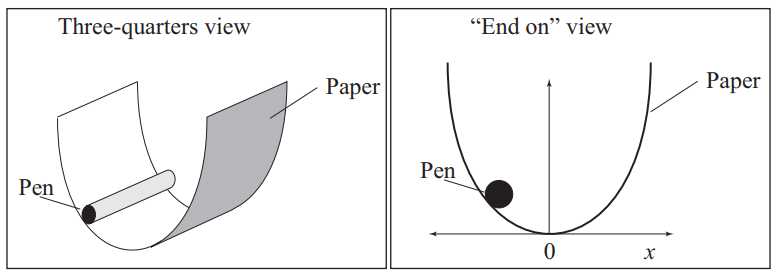
\includegraphics[height=0.3\textwidth]{img/2017S1.png}
\end{center}
When you do this experiment, the horizontal position of the pen ($x$ in the sketch on the right) is a function of time $t$, and obeys the following equation (assuming conservation of energy)
\[
\ddot x = \frac{-f'(x)}{a(1 + f'(x))}- \frac{f''(x)}{2(1+f'(x))}\left(\dot x \right)^2,
\]
where $f(x)$ is a function that gives the height of the paper (in $m$) as a function of $x$ (you may assume it and all of its derivatives are continuous), and $a$ is a constant with units of $s^2 / m$. Note that the dot indicates a time derivative and prime indicates a derivative with respect to $x$, which is measured in $m$.
\begin{itemize}
    \item[\textbf{(a)}] Find all fixed points and determine their stability (your answer should depend on $a$, $f(x)$, and/or its derivatives). Note, for this question, use the Lyapunov definition of stability, where a fixed point is stable if trajectories that start sufficiently close (but not exactly at) the fixed point remain within some small neighborhood of the fixed point. You may assume that there is no point at which $f'(x) = f''(x) = 0$.
    
    \item[\textbf{(b)}] You might expect that the pen will oscillate about a stable fixed point. Find the period of this oscillation (your answer should depend on $a$, $f(x)$ and/or its derivatives). Your answer should include units.
\end{itemize}
\end{qbox}
\begin{enumerate}
    \item We label $\dot x = y$ and convert this to a system of two equations:
    \[
    \begin{cases}
    \dot x = y \\
    \dot y = \frac{-f'(x)}{a(1 + f'(x))}- \frac{f''(x)}{2(1+f'(x))}y^2
    \end{cases}
    \]
    So, we require $\dot x = 0$, which then yields $f'(x) = 0$ from the $\dot y$ equation. So, our only fixed points are $(x, \dot x) = (\bar x, 0)$, where $\bar x$ is such that $f'(\bar x) = 0$. Now, we compute the Jacobian of this system:
    \begin{align*}
        J &= \mtx{cc}{0 & 1 \\
        \frac{af''(x)(1 + f'(x)) + af'(x)f''(x)}{\left[a(1 + f'(x))\right]^2} & \frac{-2f''(x)}{2(1 + f'(x))}y}
        \\
        J\big\vert_{\bar x, 0} &= \mtx{cc}{0 & 1 \\
        \frac{f''(\bar x)}{a} & 0 }
    \end{align*}
    The characteristic equation of this matrix is
    \begin{align*}
        \lambda^2 + \frac{f''(\bar x)}{a} &= 0 \so \lambda = \pm\sqrt{-\frac{f''(\bar x)}{a}}
    \end{align*}
    If $f''(\bar x)$ and $a$ have the same sign, then this is a linear center, and since our system is conservative, this would mean that the fixed point is stable. However, if $f''(\bar x)$ and $a$ have opposite signs, then this point is a saddle and thus unstable. 
    
    If we can assume our problem takes the form of the plain-text description, then we have that $f''(\bar x) > 0$ everywhere. Moreover, if we assume that $a > 0$, since $a$ is measured in squared seconds per meter, all of which units should always be nonnegative, then we can say that this fixed point is always a linear center and thus stable.
\end{enumerate}

\item \begin{qbox}
Suppose you are studying the interaction of two proteins. The concentration of the
first protein is $p(t)$ and the concentration of the second protein is $w(t)$. They interact via the
following equations:
\begin{align*}
\dot p &= A_p \frac{p^2}{K_p^2 + p^2} - kwp \\
\dot w &= A_w \frac{w}{K_w^2 + w} - kwp
\end{align*}
In each equation, the first term models the formation of protein, and the second term models the breakdown of the protein. Concentration is measured in units of number per liter and time is measured in seconds. The constants $K_p$ and $K_w$ then have units of concentration; the constants $A_p$ and $A_w$ have units of concentration per second; and $k$ has units of inverse
concentration per second.
\begin{itemize}
    \item[\textbf{(a)}] Suppose that you know $K_p/K_w = \epsilon$ (where $\epsilon$ is a small number), $A_w /(K^2_pk) = \alpha / \epsilon$ (where $\alpha$ is of order 1) and $A_p/(K^2_pk) = \beta$ (where $\beta$ is of order 1). Non-dimensionalize the equations and write them in terms of the appropriate non-dimensional variables and the nondimensional constants $\epsilon,\alpha$ and $\beta$.
    
    \item[\textbf{(b)}] Simplify the equations by expanding in $\epsilon$ and neglecting all terms of order $\epsilon$.
    
    \item[\textbf{(c)}] Identify all fixed points and determine their stability. Discuss any bifurcations that may occur.
    
    \item[\textbf{(d)}] Sketch a phase portrait of the system. On your plot, be sure to (1) identify and classify all fixed points, (2) draw all nullclines, (3) indicate the qualitative flow direction, and (4) sketch a few sample trajectories.
\end{itemize}
\end{qbox}
\begin{enumerate}
    \item We define some characteristic concentration scale $c_c$ and a characteristic time scale $t_c$. Then, our equations become:
    
    \begin{align*}
        \frac{c_c}{t_c}\dot{\widetilde p} &= A_p \frac{c_c^2\widetilde p^2}{K_p^2 + c_c^2\widetilde p^2} - kc_c^2 \widetilde w \widetilde p 
        &\ 
        \frac{c_c}{t_c}\dot{\widetilde w} &= A_w \frac{c_c\widetilde w}{K_w + c_c\widetilde w} - kc_c^2 \widetilde w \widetilde p
        \\
        \dot{\widetilde p} &= \frac{A_pt_c}{c_c} \cdot \frac{\widetilde p^2}{(K_p/c_c)^2 + \widetilde p^2} - kt_cc_c \widetilde w \widetilde p 
        &\ 
        \dot{\widetilde w} &= \frac{A_wt_c}{c_c} \cdot \frac{\widetilde w}{K_w/c_c + \widetilde w} - kt_cc_c \widetilde w \widetilde p
    \end{align*}
    We set $c_c/t_c = K_p^2k$, and our equations become
    \begin{align*}
        \dot{\widetilde p} &= \beta \cdot \frac{\widetilde p^2}{(K_p/c_c)^2 + \widetilde p^2} - \frac{c_c^2}{K_p^2}\cdot \widetilde w \widetilde p 
        &\ 
        \dot{\widetilde w} &= \frac{\alpha}{\epsilon} \cdot \frac{\widetilde w}{K_w/c_c + \widetilde w} - \frac{c_c^2}{K_p^2}\cdot \widetilde w \widetilde p
    \end{align*}
    Now, we set $c_c = K_p$. Our equations become
    \begin{align*}
        \dot{\widetilde p} &= \beta \cdot \frac{\widetilde p^2}{1 + \widetilde p^2} - \widetilde w \widetilde p 
        &\ 
        \dot{\widetilde w} &= \frac{\alpha}{\epsilon} \cdot \frac{\widetilde w}{1/\epsilon + \widetilde w} - \widetilde w \widetilde p
    \end{align*}
    So, dropping our tildes and rearranging our epsilons, we have the nondimensional equations
    \begin{align*}
        \dot{p} &= \frac{\beta p^2}{1 + p^2} - w p  \\
        \dot{w} &= \frac{\alpha w}{1 + \epsilon w} - w p.
    \end{align*}
    
    \item Our simplified equations are
    \begin{align*}
        \dot{p} &= p\left(\frac{\beta p}{1 + p^2} - w\right)  \\
        \dot{w} &= w\left(\alpha - p\right).
    \end{align*}
    
    \item Our first fixed point is $(p, w) = (0, 0)$. Our other is $(p, w) = (\alpha, \beta \alpha / (1 + \alpha^2))$. To find their stability, we compute the Jacobian:
    \begin{align*}
        J &= \mtx{cc}{-w + \frac{2\beta p}{(1 + p^2)^2} & -p \\ -w & \alpha - p}
        \\
        J \big\vert_{0,0} &= \mtx{cc}{0 & 0 \\ 0 & \alpha}
    \end{align*}
    So, for $(0, 0)$, our eigenvalues are $\lambda = 0, \alpha$. Since $\alpha \geq 0$, we classify this fixed point as unstable everywhere except $\alpha = 0$, in which case we cannot determine the stability. Now, we check our other fixed point:
    \begin{align*}
        J\big\vert_{\alpha, w(\alpha)} &= \mtx{cc}{\frac{\alpha\beta(1-\alpha)}{(1 + \alpha^2)^2} & -\alpha \\ -\frac{\alpha\beta}{1 + \alpha^2} & 0}
    \end{align*}
    We compute the eigenvalues:
    \begin{align*}
        \left(\frac{\alpha\beta(1-\alpha)}{(1 + \alpha^2)^2} - \lambda\right)(-\lambda) - \frac{\alpha^2\beta}{1 + \alpha^2} &= 0 \\
        \lambda^2 - \lambda \frac{\alpha\beta(1-\alpha)}{(1 + \alpha^2)^2} - \frac{\alpha^2\beta}{1 + \alpha^2} &= 0
    \end{align*}
    By the quadratic formula, we get
    \begin{align*}
        \lambda &= \frac{\alpha\beta(1-\alpha)}{2(1 + \alpha^2)^2} \pm \frac{1}{2}\sqrt{\left(\frac{\alpha\beta(1-\alpha)}{(1 + \alpha^2)^2}\right)^2 + 4\frac{\alpha^2\beta}{1 + \alpha^2}}
        \\
        &= \frac{\alpha\beta(1-\alpha)}{2(1 + \alpha^2)^2} \pm \frac{1}{2}\sqrt{\frac{\alpha^2\beta^2(1-\alpha)^2 + 4\alpha^2\beta (1 + \alpha)^3}{(1 + \alpha^2)^4}}
        \\
        &= \frac{\alpha\beta(1-\alpha)}{2(1 + \alpha^2)^2} \pm \frac{\alpha}{2(1+\alpha^2)^2}\sqrt{\beta^2(1-\alpha)^2 + 4\beta (1 + \alpha)^3}
        \\
        &=
        \frac{\alpha}{2(1+\alpha^2)^2}\left(\beta(1-\alpha) \pm \sqrt{\beta^2(1-\alpha)^2 + 4\beta (1 + \alpha)^3}\right)
    \end{align*}
    To illuminate what's going on, we'll label $\beta(1-\alpha) = \gamma$. Then, our eigenvalues are
    \[
    \lambda = \frac{\alpha}{2(1+\alpha^2)^2}\left(\gamma \pm \sqrt{\gamma^2 + 4\beta (1 + \alpha)^3}\right)
    \]
    Since $\alpha, \beta \geq 0$, if we look at these values in terms of positive and negative values $(+), (-)$, we have
    \[
    \lambda = \alpha (+)\left(\gamma \pm \sqrt{\gamma^2 + \beta(+)}\right)
    \]
    If $\alpha$ or $\beta = 0$, then we won't be able to tell anything about these eigenvalues, but otherwise, we have that the object under our radical is always real and greater than $\gamma$, and so one eigenvalue will always be positive and the other will be negative. Therefore, this point is a saddle, so it is unstable.
    
    The only possible point where a bifurcation may occur is when $\alpha = 0$ or $\beta = 0$. When $\alpha = 0$, our two fixed points merge into one, but since $\alpha$ is always nonnegative, it doesn't truly make sense to consider this as a bifurcation so much as an edge case. If we \textbf{did} want to consider mathematically valid but physically invalid values of $\alpha, \beta$, then this would probably correspond with a transcritical bifurcation, since both of our fixed points would pass through each other but still exist. Similarly, if we were to look at what happens when $\beta$ passes through 0 and becomes negative, then the eigenvalues associated with the fixed point not at the origin would change shape and/or stability. There could be a bifurcation in here, like perhaps a Hopf bifurcation.
    
    \item We find the $p, w$ nullclines first.
    
    $\dot p = 0$ gives the following cases: we can have $p = 0$, in which case $\dot w = \alpha w > 0$, or we can have
    \begin{align*}
        w &= \frac{\beta p}{1 + p^2} \so \dot w = \begin{cases}
        (+) &p < \alpha \\ 0 & p = \alpha \\ (-) &p > \alpha 
        \end{cases}
    \end{align*}
    If $\dot w = 0$, then we can have $w = 0$, in which case $\dot p = \beta p^2/(1 + p^2)$, or we can have 
    \begin{align*}
        p &= \alpha \so \dot p = \alpha\left(\frac{\alpha \beta}{1 + \alpha^2} - w\right) = \begin{cases}
        (+) &w < \frac{\alpha \beta}{1 + \alpha^2} \\ 0 & w = \frac{\alpha \beta}{1 + \alpha^2} \\ (-) &w > \frac{\alpha \beta}{1 + \alpha^2} 
        \end{cases}
    \end{align*}
    So, we get the following phase plane:
    \begin{center}
    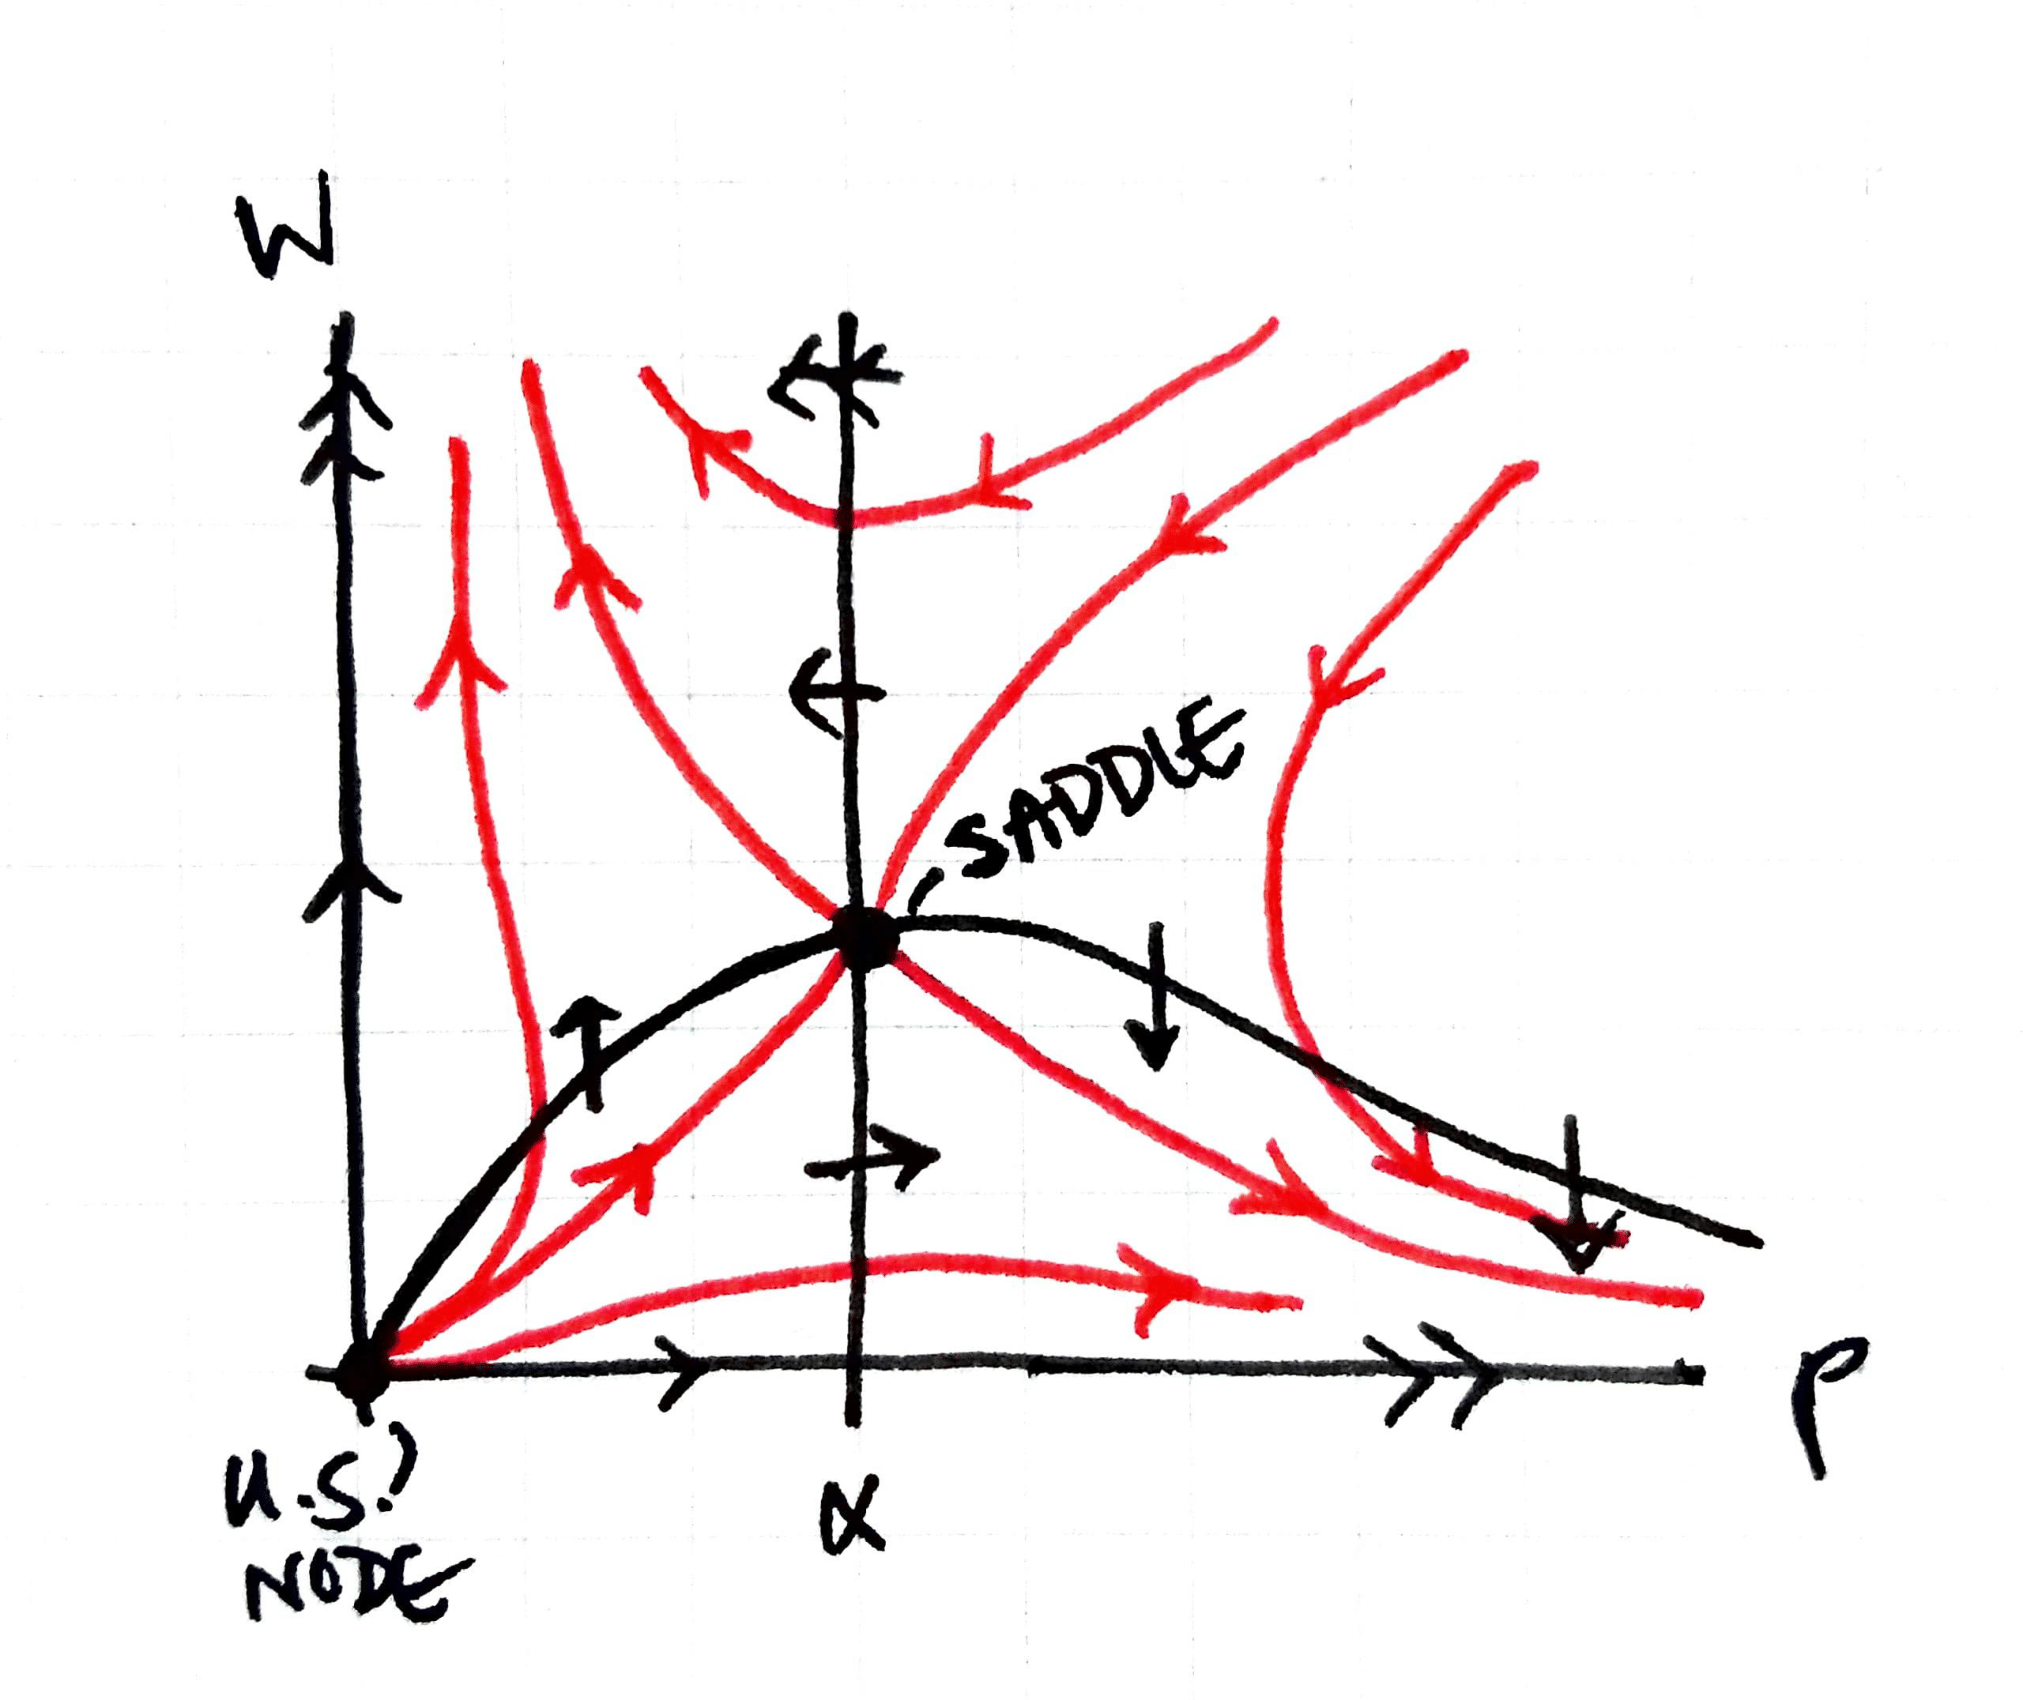
\includegraphics[height=0.3\textwidth]{img/2017S2.png}
    \end{center}
\end{enumerate}

\item \begin{qbox}
Let $L$ be the differential operator
\[
Lu = (1 + x^2)u'' - 2xu' \qquad 0 < x < 1
\]
with boundary conditions $Bu = 0$ given by $u'(0) = 0$, $u'(1) = 0$.
\begin{itemize}
    \item[\textbf{(a)}] Find the adjoint $L^*$ of $L$ in $L^2(0, 1)$ and the adjoint boundary conditions $B^*u = 0$.
    
    \item[\textbf{(b)}] What are the solutions of the homogeneous boundary value problem $Lu = 0$, $Bu = 0$? What is the dimension of the null space?
    
    \item[\textbf{(c)}] What are the solutions of the homogeneous adjoint boundary value problem $L^*u = 0$, $B^*u = 0$? What is the dimension of the null space?
\end{itemize}
\end{qbox}
\begin{enumerate}
    \item We want to find $L^*$ such that $\ip{Lu}{w} = \ip{u}{L^* w}$.
    \begin{align*}
        \ip{Lu}{w} &= \int_0^1\left[(1+x^2)u'' - 2xu'\right]w\,dx
        =
        \undernum{\int_0^1(1+x^2)u''w\,dx}{1} - \undernum{\int_0^12xu'w\,dx}{2}
    \end{align*}
    First, we examine $\circled 1 :$
    \begin{align*}
        \circled 1 &= \int_0^1(1+x^2)u''w\,dx \\
        &= (1 + x^2)wu'\big\vert_0^1 - \int_0^1 u'\left[2xw + (1+x^2)w'\right]\,dx &\textrm{(IBP)}
        \\
        &= - \int_0^1 u'\left[2xw + (1+x^2)w'\right]\,dx &\textrm{(Boundary Conditions)}
        \\
        &= -u(2xw + (1+x^2)w')\bigg\vert_0^1 + \int_0^1 u\left[2w + 4xw' + (1+x^2)w''\right]\,dx &\textrm{(IBP)}
        \\
        &= -2u(1)\left(w(1)+w'(1)\right) + u(0)w'(0) + \int_0^1 u\left[2w + 4xw' + (1+x^2)w''\right]\,dx
    \end{align*}
    Next, we examine $\circled 2:$
    \begin{align*}
        \circled 2 &= 
        \int_0^12xu'w\,dx \\
        &= 
        2w(1)u(1) -  \int_0^1 2(w + xw')u\,dx &\textrm{(IBP)}
    \end{align*}
    Putting these together, we get
    \begin{align*}
        \ip{Lu}{w} &= \circled 1 - \circled 2
        \\
        &= -2u(1)\big[2w(1) + w'(1)\big] + u(0)w'(0) + \int_0^1 u\left[4w + 6xw' + (1+x^2)w''\right]\,dx
    \end{align*}
    So, our adjoint operator is given by
    \[
    L^* u = 4u + 6xu' + (1+x^2)u''
    \]
    with boundary conditions $2u(1) + u'(1) = 0$ and $u'(0) = 0$.
    
    \item Setting $Lu = 0$, we get
    \begin{align*}
        (1+x^2)u'' - 2xu' &= 0 \\
        (1+x^2)u'' &= 2xu' \\
        \frac{u''}{u'} &= \frac{2x}{1 + x^2} \\
        \ln u' &= \ln (1 + x^2) + C \\
        u' &= C(1 + x^2) \\
        u &= C\left(x + \frac{1}{3}x^3\right) + D
    \end{align*}
    The boundary condition $u'(0) = 0$ gives $C = 0$, and $u'(1) = 0$ gives the same. So, we get $u = D \in \R$ is the solution. The nullspace has dimension 1, since we have only one degree of freedom.
    
    \item Setting $L^*u = 0$, we get
    \begin{align*}
        (1+x^2)u'' + 6xu' + 4u &= 0 \\
        \big[(1+x^2)u'' + 2xu'\big] +\big[ 4xu' + 4u \big] &= 0 \\
        \frac{d}{dx}\left[(1+x^2)u'\right] + \frac{d}{dx}\big[4ux\big] &= 0
        \\
        \frac{d}{dx}\left[(1+x^2)u' + 4ux\right] &= 0
        \\
        (1+x^2)u' + 4ux &= C
        \\
        u' + \frac{4x}{1+x^2}u &= \frac{C}{1+x^2}
    \end{align*}
    Now, we use an integrating factor:
    \[
    \mu(x) = \int\frac{4x}{1+x^2}\,dx = 2\ln\abs{1+x^2} \so e^{\mu(x)} = (1+x)^2
    \]
    This yields
    \begin{align*}
        u(x) &= \frac{1}{(1+x^2)^2}\int(1+x^2)^2\cdot\frac{C}{1+x^2}\,dx
        \\
        &=
        \frac{1}{(1+x^2)^2}\int C(1+x^2)\,dx
        \\
        &=
        \frac{1}{(1+x^2)^2}\left[C\left(x + \frac{1}{3}x^3\right) + D\right]
    \end{align*}
    We plug in the boundary condition $u'(0) = 0:$
    \begin{align*}
        u'(x) &= \frac{C(1+x^2)(1+x^2)^2 - (C(x+x^3/3)+D)4x(1+x^2)}{(1+x^2)^4}
        \\
        u'(0) &= C = 0
    \end{align*}
    So, we have 
    \[
    u(x) = \frac{D}{(1+x^2)^2}.
    \]
    Plugging in the boundary condition $2u(1)+u'(1) = 0$ yields
    \[
    2D - 4D = 0 \so D = 0.
    \]
    So, the only solution is the trivial solution. So the nullspace has dimension 0.
\end{enumerate}

\item 
\begin{qbox}
\begin{itemize}\vspace{-1.5em}
\item[\textbf{(a)}] Let $\Omega = \{(x, y) \in \R^2 : -a < x < a,\ 0 < y < b\}$ be a rectangle. Use separation of variables to solve the boundary value problem
\begin{align*}
    u_{xx} +u_{yy} &= 0, \qquad  (x, y) \in \Omega \\
    u(x, 0) &= 0, \qquad  u(x,b) = e^{-x^2}, \\
    u_x(-a, y) &= 0, \qquad  u_x(a, y) = 0.
\end{align*}
\item[\textbf{(b)}] What is a physical interpretation of this problem? What is the approximate limiting behavior of the solution as $b \to 0$? 
\end{itemize}
\end{qbox}
\begin{enumerate}
\item 
We let $u(x, y) = X(x)Y(y)$. Then, our PDE has the form
\[
X''Y + XY'' = 0 \so \frac{X''}{X} = -\frac{Y''}{Y} = \lambda.
\]
We show that $\lambda$ is nonnegative.
\begin{align*}
    X'' &= \lambda X \\
    X''X &= \lambda X^2 \\
    X'X\big\vert_{-a}^a - \int(X')^2 &= \lambda \int X^2 &\textrm{(IBP)}
    \\
    - \int(X')^2 &= \lambda \int X^2 &\textrm{(Boundary Condition)} 
\end{align*}
So, $\lambda = -\mu^2$. We now solve our $X$ equation:
\begin{align*}
    X'' = -\mu^2 X \so X &= A\sin(\mu x) + B\cos(\mu x) \\
    X' &= \mu\left[A\cos(\mu x) - B\sin(\mu x)\right]
\end{align*}
Plugging in our boundary condititions yields
\begin{align*}
    X'(a) &= \mu\left[A\cos(\mu a) - B\sin(\mu a)\right] = 0 \\
    X'(-a) &= \mu\left[A\cos(\mu a) + B\sin(\mu a)\right] = 0
\end{align*}
So, we have
\[
A\cos(\mu a) = B\sin(\mu a) = 0.
\]
This gives us two possible conditions:
\begin{align*}
    (1)\quad  B &= 0 \quad\textrm{and}\quad \mu a = (k + 1/2)\pi \\
    (2)\quad  A &= 0 \quad\textrm{and}\quad \mu a = k\pi 
\end{align*}
That is, for all $k \in \N$,
\begin{align*}
    (1)\quad X_k(x) &= \sin(\mu_k x), \qquad \mu_k = \frac{\pi}{a}\left(k + \frac{1}{2}\right)
    \\
    (2)\quad X_k(x) &= \cos(\widetilde \mu_k x), \qquad \widetilde \mu_k = \frac{k\pi}{a}.
\end{align*}
Now we solve our $Y$ equation:
\begin{align*}
    -\frac{Y'}{Y} = -\mu^2 \so
    Y'' = \mu^2 Y \so
    Y(y) = Ce^{\mu y} + De^{-\mu y}
\end{align*}
The boundary condition $Y(0) = 0$ gives $D = -C$, and so we get
\[
Y_k(y) = C_k\left(e^{\mu_k y} - e^{-\mu_k y}\right).
\]
Now, we plug in the boundary condition at $y = b$, combining our two cases for the $X_k$:
\[
u(x, b) = e^{-x^2} = \sum_{k \in \N}\left[ C_k\left(e^{\mu_k b} - e^{-\mu_k b}\right) \sin(\mu_k x) + \widetilde C_k\left(e^{\widetilde \mu_k b} - e^{-\widetilde \mu_k b}\right) \cos(\widetilde \mu_k x)\right]
\]
Note that since $e^{-x^2}$ is an even function, the sines should not play into the solution at all. So, we actually collapse to case (2), dropping the tildes now since we are only dealing with one value of $\mu_k$:
\begin{align*}
    e^{-x^2} &= \sum_{k \in \N} C_k\left(e^{\mu_k b} - e^{-\mu_k b}\right) \cos(\mu_k x)
\end{align*}
Our coefficients are then given by
\begin{align*}
    C_k = \frac{\ip{\cos(\mu_k x)}{e^{-x^2}\left(e^{\mu_k b} - e^{-\mu_k b}\right)^{-1}}}{\ip{\cos(\mu_k x)}{\cos(\mu_k x)}}
\end{align*}
First, we compute the norm of our basis functions:
\begin{align*}
    \ip{\cos(\mu_k x)}{\cos(\mu_k x)}
    &=
    \int_{-a}^a \cos^2\left(\frac{k \pi}{a} x\right)\,dx
    \\
    &=
    \frac{a}{\pi} \int_{-\pi}^\pi \cos^2(k\theta)\,d\theta &(\textrm{u-sub: }\theta = \pi x/a)
    \\
    &= \frac{a}{\pi} \cdot \frac{1}{2}(2\pi)
    \\
    &= a
\end{align*}
So, we now have 
\begin{align*}
    C_k &= \frac{1}{a}\ip{\cos(\mu_k x)}{e^{-x^2}\left(e^{\mu_k b} - e^{-\mu_k b}\right)^{-1}}
    \\
    &=
    \frac{1}{a}\left(e^{\mu_k b} - e^{-\mu_k b}\right)^{-1}\int_{-a}^a e^{-x^2}\cos(\mu_k x)\,dx,\qquad \textrm{where}\quad \mu_k = \frac{k\pi}{a}
\end{align*}
So, our final solution (with the $C_k$ and $\mu_k$ as given above) is
\[
u(x, y) = \sum_{k \in \N} C_k \left(e^{\mu_k y} - e^{-\mu_k y}\right) \cos(\mu_k x).
\]
\item This is Laplace's equation on a rectangle, where we are fixed along the $y$-boundaries and are flat in the $x$-direction across the $x$-boundaries. As $b \to 0$, our constants $C_k$ approach 0, so the solution approaches 0.
\end{enumerate}

\addtocounter{enumi}{1}

\item \begin{qbox}
The dimensionless equation of motion of a frictionless pendulum is
\[
\frac{d^2\theta}{dt^2} + \sin\theta = 0.
\]
In the limit of small amplitude (e.g. denote the amplitude of the $\theta$ as $\epsilon$), the period is $2\pi$ to leading order. Compute the next term in the expansion of the period for small amplitude.
\end{qbox}

(With help from Wai Ho Chak and Lifeng Ren)

We begin by multiplying each side of our equation by $\dot \theta$ and integrating with respect to $t$:
\begin{align*}
    \ddot \theta &= -\sin\theta \\
    \ddot\theta\dot\theta &= -\sin\theta\cdot \dot\theta \\
    \frac{1}{2}\left(\dot\theta\right)^2 &= \cos\theta + C \\
    \dot\theta^2 &= 2\left(\cos\theta + C\right)
    \\
    \dot\theta &= \sqrt 2 \cdot \sqrt{\cos\theta + C}
\end{align*}
Since the amplitude of $\theta(t)$ is $\epsilon$, without loss of generality, we take $\dot \theta(0) = 0$ and $\theta(0) = \epsilon$. Together, these give
\[
\dot\theta(0) = 0 \so \cos(\theta(0)) + C = 0 \so C = -\cos \epsilon.
\]
So, we now have
\[
\dot\theta = \sqrt 2 \cdot \sqrt{\cos\theta -\cos \epsilon}.
\]
Since we want to find the amount of time it takes to go from one state where $\dot \theta = 0$ back to that original state, what we're trying to find is how much time it takes for $\theta$ to pass from $\epsilon$ to $0$ to $-\epsilon$ to $0$ and back to $\epsilon$. Due to the symmetry of the problem, this is equivalent to 4 times the time $\theta$ takes to pass from $0$ to $\epsilon$, and so
\[
T(\epsilon) = 4\int_0^{\epsilon}\frac{1}{\dot \theta}\,d\theta = 4\int_0^\epsilon \frac{\sqrt{2}}{2}\cdot \frac{d\theta}{\sqrt{\cos\theta - \cos \epsilon}} = 2\sqrt 2 \int_0^\epsilon \frac{d\theta}{\sqrt{\cos\theta - \cos \epsilon}}.
\]
We know that, for our above expression, $0 < \theta < \epsilon$ where $\epsilon$ is small. So,
\begin{align*}
    T(\epsilon)
    &=
    2 \sqrt 2 \int_0^\epsilon \frac{d\theta}{\sqrt{\cos\theta - \cos \epsilon}}
    \\
    &=
    2 \sqrt 2 \int_0^\epsilon \left[\left(\frac{\epsilon^2 - \theta^2}{2}\right) - \left(\frac{\epsilon^4 - \theta^4}{4!}\right) + \Ord{\epsilon^6}\right]^{-1/2}\,d\theta
    \\
    &=
    2 \sqrt 2 \int_0^\epsilon \left(\frac{\epsilon^2 - \theta^2}{2}\right)^{-1/2}\left(1 - \left(\frac{\epsilon^2 + \theta^2}{12}\right) + \Ord{\epsilon^4}\right)^{-1/2}\,d\theta
    \\
    &=
    2 \sqrt 2 \int_0^\epsilon \sqrt{\frac{2}{\epsilon^2 - \theta^2}}\left[1 + \frac{\epsilon^2 + \theta^2}{24} + \Ord{\epsilon^4}\right]\,d\theta
    \\
    &=
    4 \undernum{\int_0^\epsilon \frac{d\theta}{\sqrt{\epsilon^2 - \theta^2}}}{1} + \frac{1}{6}\undernum{\int_0^\epsilon\frac{\epsilon^2 + \theta^2}{\sqrt{\epsilon^2 - \theta^2}}\,d\theta}{2} + \Ord{\epsilon^4}
\end{align*}
Examining $(1)$ and $(2)$, we have
\begin{align*}
    (1) &:\quad \int_0^\epsilon \frac{d\theta}{\sqrt{\epsilon^2 - \theta^2}} = \int_0^{\pi/2}d\phi = \frac{\pi}{2} \qquad \left(\textrm{using }\theta = \epsilon\sin\phi,\ d\theta = \epsilon\cos\phi\,d\phi\right)
    \\
    (2) &:\quad \int_0^a\frac{\epsilon^2 + \theta^2}{\sqrt{\epsilon^2 - \theta^2}}\,d\theta
    =
    \int_0^{\pi/2}\epsilon^2(1+\sin^2\phi)\,d\phi 
    =
    \epsilon^2\int_0^{\pi/2}\left[ 1 + \frac{1 - \cos(2\phi)}{2}\right]\,d\phi
    =
    \frac{\pi \epsilon^2}{2} + \frac{\pi \epsilon^2}{4} = \frac{3\pi \epsilon^2}{4}.
\end{align*}
So, all together,
\[
T(\epsilon) = 4\left(\frac{\pi}{2}\right) + \frac{1}{6}\left(\frac{3\pi \epsilon^2}{4}\right) + \Ord{\epsilon^4} = 2\pi + \frac{\pi}{8}\epsilon^2 + \Ord{\epsilon^4} \quad \textrm{as }\epsilon\to 0.
\]


\end{enumerate}

\chapter*{Fall 2016}
\chaptermark{Fall 2016}
\addcontentsline{toc}{chapter}{Fall 2016}

\begin{enumerate}
\item
\begin{qbox}
The SIR model is a simple and sometimes accurate way to describe the spread of a
disease in a population. One variant of the model is given by the following three equations:
\begin{align*}
\frac{dS}{dt} &= a(I +R +S) - aS - bS I \\
\frac{d I}{dt} &= bS I - a I - c I \\
\frac{dR}{dt} &= c I - aR
\end{align*}
where $S$ is the number of susceptible individuals, $I$ the number of infected individuals and $R$ the number of recovered individuals in the population and $t$ is time.

The parameters are defined as follows:

$a$ is the birth rate and also the death rate. Since these rates are equal, the population maintains a constant size, $R + I +S = N$, where $N$ is a constant.

$b$ is the transmission likelihood. When a susceptible and infected individual meet, the susceptible becomes infected with some probability. The parameter $b$ defines the rate that susceptible and infected individuals meet and the infection is transmitted.

$c$ is the recovery rate. An infected individual recovers at this rate, and then is immune to the
disease.

\begin{itemize}
    \item[\textbf{(a)}] Using $a$ and $N$ to define your time and population scales, respectively, non-dimensionalize the three differential equations.
    
    Given the appropriate non-dimensionalization, and using the constraint that the population maintains a constant size, the equations become
    \begin{align*}
        \frac{dx}{dT} &= 1 - x - \alpha x y \\
        \frac{dy}{dT} &= \alpha x y - (1 + \beta) y
    \end{align*}
    where $x$ is the probability that an individual is susceptible, $y$ is the probability that an individual is infected, and the probability that an individual is resistant ($z$) can be determined from the constraint $x + y + z = 1$.
    
    \item[\textbf{(b)}] Find all fixed points $(x^*, y^*)$ and determine their stability for all combinations of $\alpha, \beta > 0$.
    
    \item[\textbf{(c)}] Suppose that $\beta = 1$. A bifurcation occurs as $\alpha$ changes. Classify this bifurcation, and sketch a phase portrait before and after the bifurcation.
\end{itemize}
\end{qbox}

\begin{enumerate}
    \item We use $N$ as our population scale and $1/a$ as our time scale. Then, our first equation becomes
    \begin{align*}
        aN \dot{\widetilde S} &= aN - aN\widetilde S - bN^2 \widetilde S \widetilde I \\
        \dot{\widetilde S} &= 1 - \widetilde S - \frac{bN}{a} \widetilde S \widetilde I
    \end{align*}
    Our second equation becomes 
    \begin{align*}
        a N \dot{\widetilde I} &= b N^2 \widetilde S \widetilde I - aN\widetilde I - c N \widetilde I \\
        \dot{\widetilde I} &= \frac{bN}{a}\widetilde S \widetilde I - \left(1 + \frac{c}{a}\right) \widetilde I
    \end{align*}
    Our third equation becomes
    \begin{align*}
        aN \dot{\widetilde R} &= c N \widetilde I - a N \widetilde R \\
        \dot{\widetilde R} &= \frac{c}{a}\widetilde I - \widetilde R
    \end{align*}
    Setting $\alpha = bN/a$ and $\beta = c/a$, we get the given set of nondimensional equations.
    
    \item We first solve for when $\dot y = 0:$
    \begin{align*}
        0 &= y\left(\alpha x - ( 1 + \beta) \right)
    \end{align*}
    This yields $y = 0$ and $x = (1 + \beta)/\alpha$. Plugging these into $\dot x = 0$, we get
    \begin{alignat*}{5}
        y &= 0 &\qquad &\rightarrow&\qquad 0 &= 1 - x &\qquad &\rightarrow&\qquad x &= 1 \\
        x &= \frac{1 + \beta}{\alpha} &\qquad &\rightarrow&\qquad 0 &= 1 - \frac{1 + \beta}{\alpha}\left(1 + \alpha y\right) &\qquad &\rightarrow&\qquad y &= \frac{\alpha - (1 + \beta)}{\alpha(1 + \beta)}
    \end{alignat*}
    So, our two fixed points are given by
    \[
    (x^*, y^*) = (1, 0),\ \left(\frac{1 + \beta}{\alpha},\frac{\alpha - (1 + \beta)}{\alpha(1 + \beta)} \right)
    \]
    For simplicity for the following computations, we label $1 + \beta = \gamma$. Then, our fixed points are equivalently 
    \[
    (x^*, y^*) = (1, 0),\ \left(\frac{\gamma}{\alpha},\frac{\alpha - \gamma}{\alpha\gamma} \right).
    \]
    The Jacobian for this system is
    \begin{align*}
        J &= \mtx{cc}{-(1+\alpha y) & -\alpha x \\ \alpha y & \alpha x - \gamma}.
    \end{align*}
    First, we compute the stability of $(1, 0):$
    \begin{align*}
        J\big\vert_{1,0} = \mtx{cc}{-1 & -\alpha \\ 0 & \alpha - \gamma}
        \so
        0 &= (-1-\lambda)(\alpha-\gamma-\lambda) \\
        0 &= \lambda^2 + \lambda(1 - \alpha + \gamma) - \alpha + \gamma \\
        \lambda &= -\frac{1}{2}\left(1 - \alpha + \gamma\right) \pm \frac{1}{2}\sqrt{(1 - \alpha + \gamma)^2 - 4(-\alpha + \gamma)}
    \end{align*}
    We first check if this value is ever complex by examining the object under the radical:
    \begin{align*}
        (1 - \alpha + \gamma)^2 - 4(-\alpha + \gamma) 
        &=
        (2 - \alpha + \beta)^2 - 4(1 -\alpha + \beta) \\
        &= 
        4 - 4\alpha + 4\beta - 2\alpha\beta + \alpha^2 + \beta^2 - 4 + 4\alpha - 4\beta
        \\
        &= \alpha^2 - 2\alpha\beta + \beta^2 \\
        &= (\alpha - \beta)^2
    \end{align*}
    Plugging this back into our expression for our eigenvalues, we have
    \begin{align*}
        \lambda &= -\frac{1}{2}\left(2 - \alpha + \beta\right) \pm \frac{1}{2}(\alpha - \beta) = -1,\ \alpha - (1 + \beta)
    \end{align*}
    So, we get the following cases:
    \begin{align*}
        (1, 0) \textrm{ is a } \begin{cases}
        \textrm{saddle} &: \alpha > 1 + \beta \\
        \textrm{stable node} &: \alpha < 1 + \beta
        \end{cases}
    \end{align*}
    Now, we check our other fixed point. 
    \begin{align*}
        J\bigg\vert_{\left(\frac{\gamma}{\alpha},\frac{\alpha - \gamma}{\alpha\gamma} \right)} = \mtx{cc}{-\frac{\alpha}{\gamma} & -\gamma \\ \frac{\alpha}{\gamma} - 1 & 0}
        \so
        0 &= \lambda^2 +\frac{\alpha}{\gamma}\lambda + \alpha - \gamma
        \\
        \lambda &= \frac{1}{2}\left[-\frac{\alpha}{\gamma} \pm \sqrt{\left(\frac{\alpha}{\gamma}\right)^2 - 4(\alpha - \gamma)}\right]
    \end{align*}
    So, we get the following cases:
    \begin{align*}
        \left(\frac{\beta + 1}{\alpha},\frac{\alpha - (\beta + 1)}{\alpha(\beta + 1)} \right) &\textrm{ is a }
        \begin{cases}
        \textrm{saddle} &: \alpha < \beta + 1 \\
        \textrm{stable node} &: \alpha > \beta + 1 \textrm{ and } \left(\frac{\alpha}{\beta + 1}\right)^2 > 4(\alpha - \beta - 1)
         \\
        \textrm{stable spiral} &: \alpha > \beta + 1 \textrm{ and } \left(\frac{\alpha}{\beta + 1}\right)^2 < 4(\alpha - \beta - 1)
        \end{cases}
    \end{align*}
    
    \item 
    When $\beta = 1$, our fixed points and their stabilities become:
    \begin{align*}
        (1, 0) &\textrm{ is a } \begin{cases}
        \textrm{saddle} &: \alpha > 2 \\
        \textrm{stable node} &: \alpha < 2
        \end{cases}
        \\
        \left(\frac{2}{\alpha},\frac{\alpha - 2}{2\alpha} \right) &\textrm{ is a }
        \begin{cases}
        \textrm{saddle} &: \alpha < 2 \\
        \textrm{stable node} &: \alpha > 2 \textrm{ and } \alpha^2 > 16(\alpha - 2)
         \\
        \textrm{stable spiral} &: \alpha > 2 \textrm{ and } \alpha^2 < 16(\alpha - 2)
        \end{cases}
    \end{align*}
    We see that when $\alpha$ passes through 2, our two fixed points collide and swap stability. So, we have a transcritical bifurcation at $\alpha = 2$.
    
    To draw the phase plane, we first note our nullclines. The $x$-nullcline is given by $x = 1/(1 + \alpha y)$. Our $y$-nullclines are given by $y = 0$ and $x = 2/\alpha$. These are the nullclines for $\alpha < 2$ and $\alpha > 2:$
    \begin{center}
    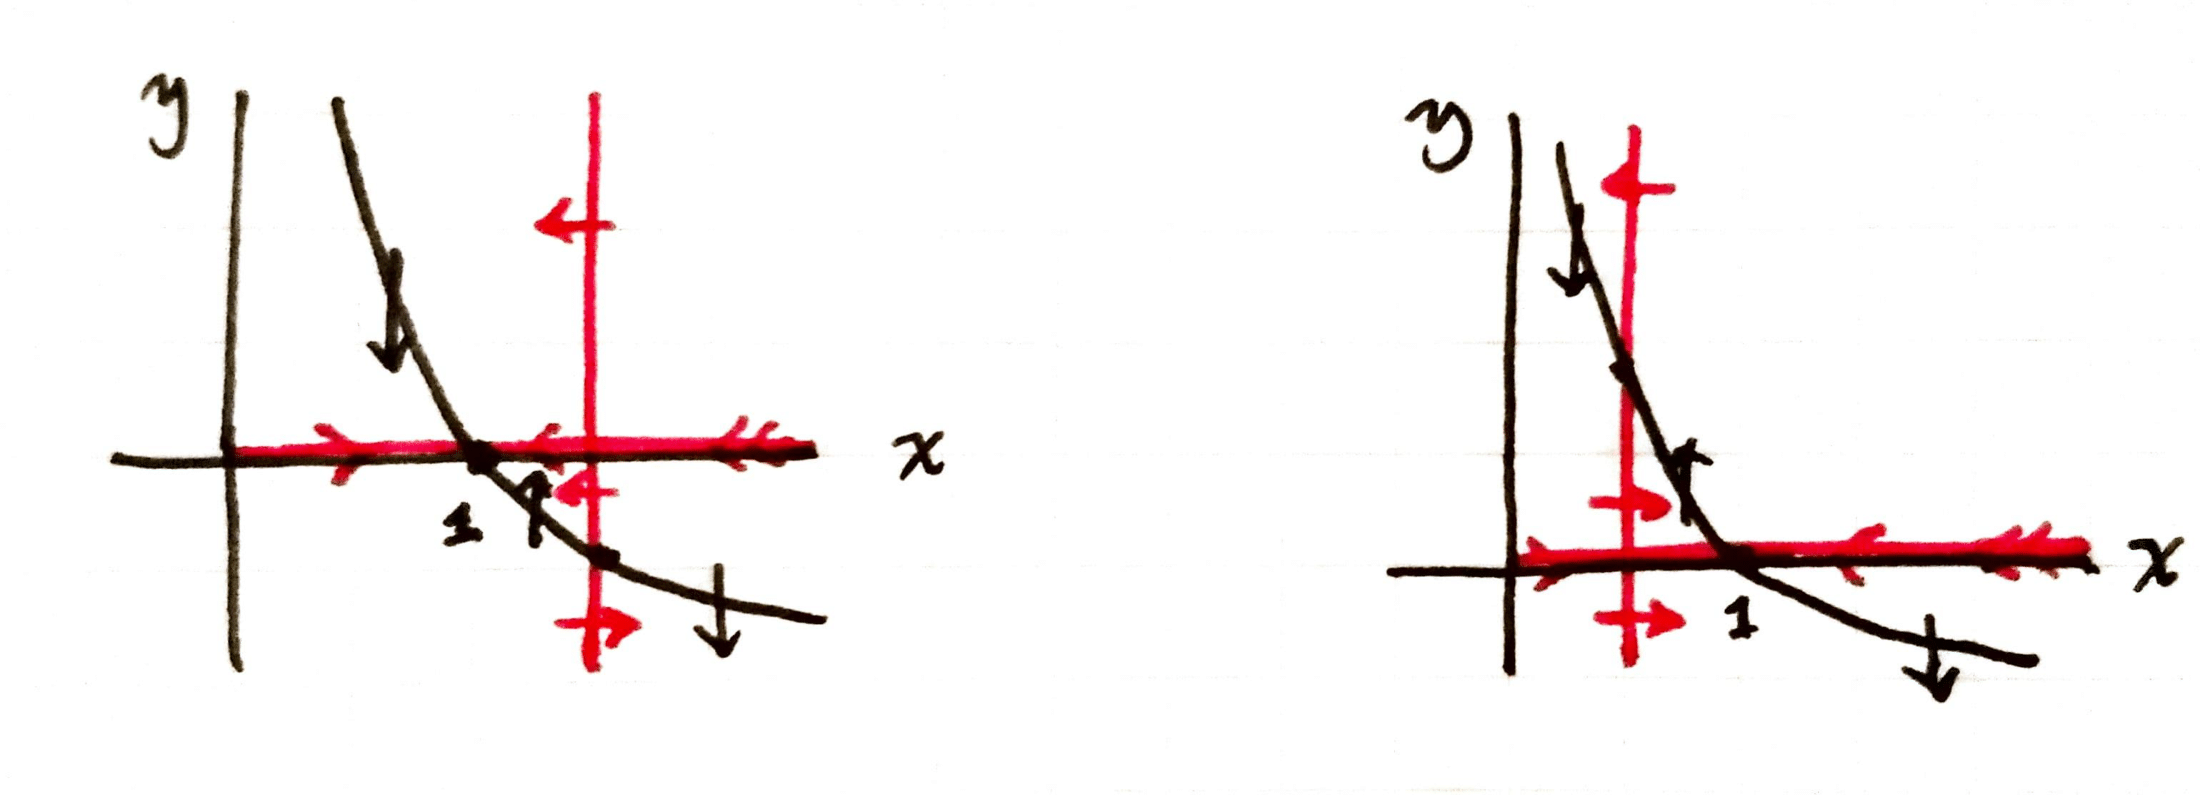
\includegraphics[height=0.275\textwidth]{Prelim/img/2016F1c1.png}
    \end{center}
    This yields the following phase planes for $\alpha < 2$ and $\alpha > 2$, respectively:
    \begin{center}
    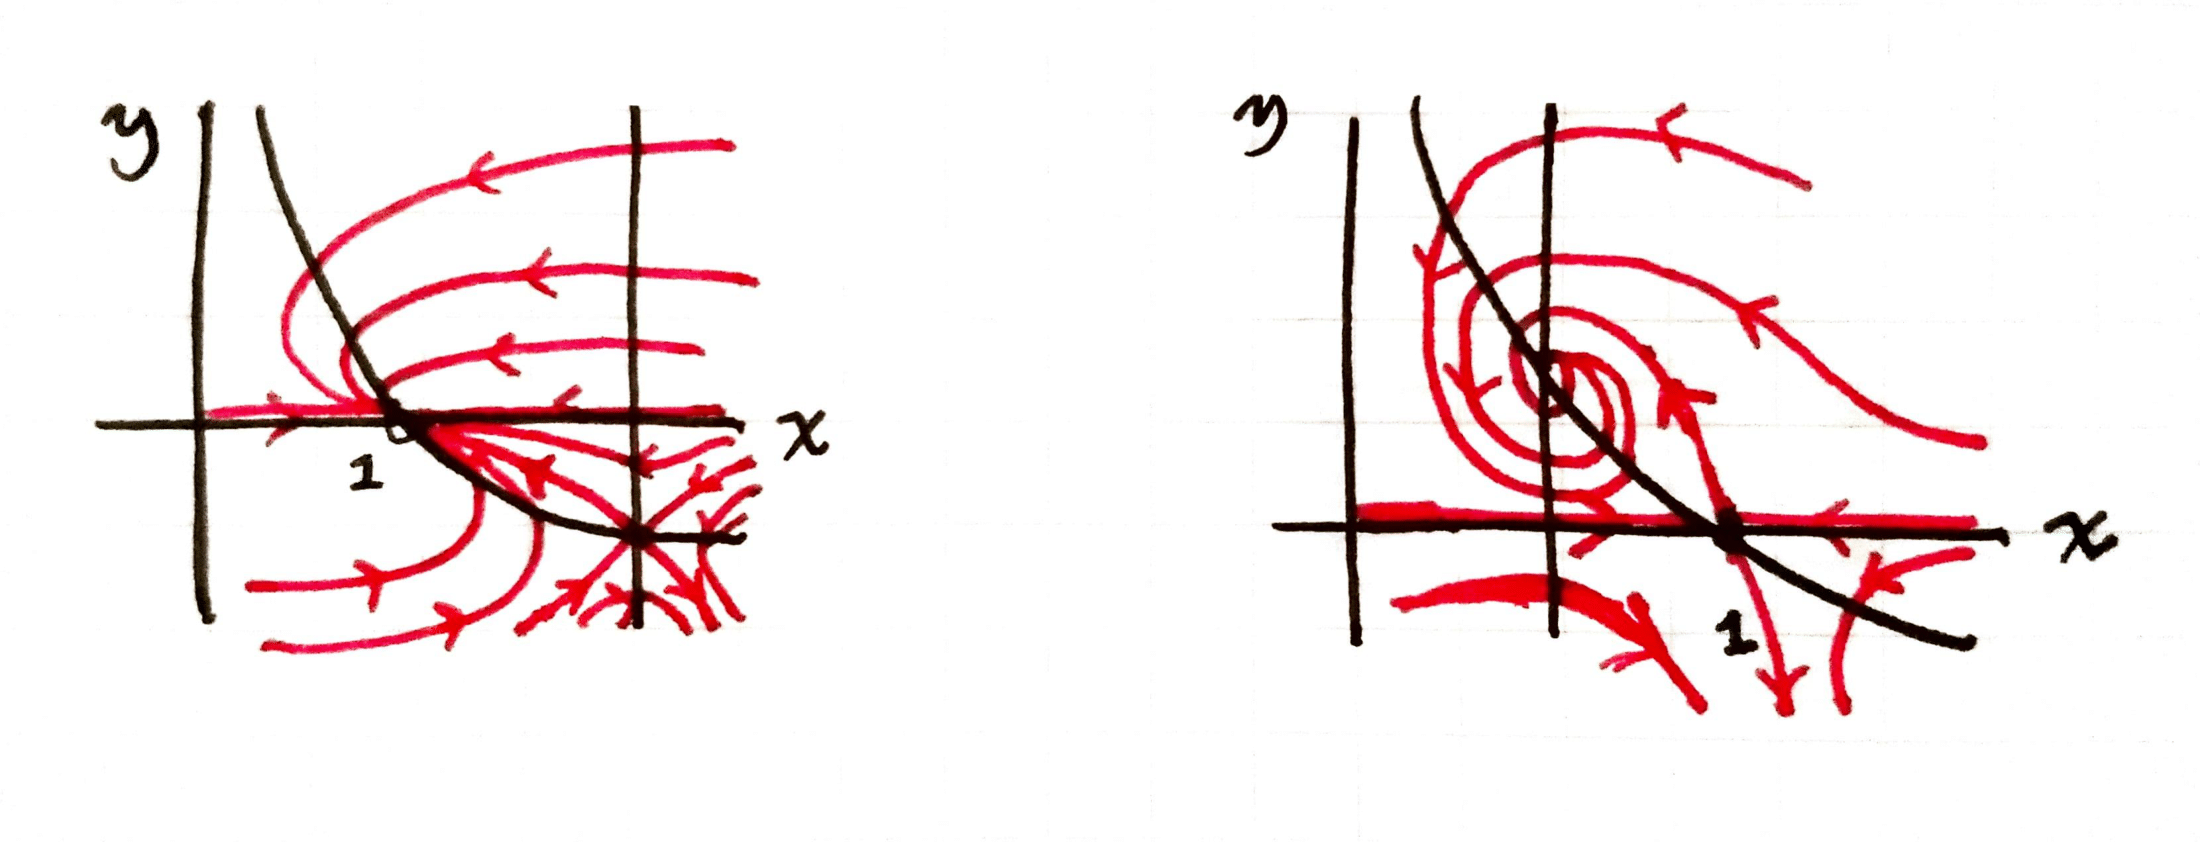
\includegraphics[height=0.285\textwidth]{Prelim/img/2016F1c2.png}
    \end{center}
\end{enumerate}

\item
\begin{qbox}
Consider the following mechanical system.
\begin{center}
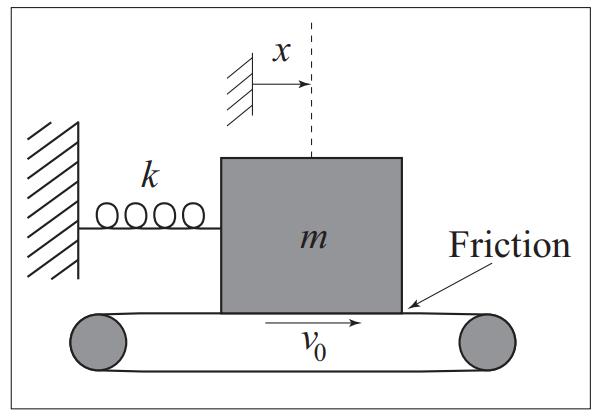
\includegraphics[height=0.25\textwidth]{Prelim/img/2016F2.png}
\end{center}
A block, of mass $m$, sits on a conveyer belt moving at velocity $v_0$. The mass is attached to a wall with a linear spring of stiffness $k$. The position of the mass, $x$, as a function of time, $t$, obeys the following differential equation:
\[
m \frac{d^2 x}{dt^2} = kx - f(\dot s),
\]
where $f$ is the frictional force that the conveyer belt applies to the block and $\dot s$ is the velocity of the block relative to the belt, $\dot s = dx/dt - v_0$. This equation can be non-dimensionalized to
\[
\frac{d^2X}{dT^2} = -X - F\left(\frac{dX}{dT} - V\right).
\]
Suppose that $V = 1$. Also, suppose that the friction force as a function of relative speed has the following form:
\[
F(x) = \begin{cases}
1 + ax &: x > 0 \\
-1 + ax &: x < 0
\end{cases}
\]
\begin{itemize}
    \item[\textbf{(a)}] Perhaps the simplest model of friction is Coulomb friction, which is the above eqn with $a = 0$. Show that linearization predicts that the unique fixed point, $X = -F(-1) = 1,\ dX/dT = 0$, is a center and explain why this is, in fact, a true center.
    
    \item[\textbf{(b)}] Show that, as $a$ varies, the fixed point goes from a stable to an unstable spiral (assuming $\abs a < 2$).
    
    \item[\textbf{(c)}] It turns out that when the fixed point becomes unstable, a limit cycle appears. This is a Hopf bifurcation. Is it a subcritical, supercritical or degenerate Hopf? Briefly (in a sentence or two) explain.
\end{itemize}
\end{qbox}

\begin{enumerate}
    \item We expand this into a system of two equations:
    \begin{align*}
        \begin{cases}
        \dot X = Y \\
        \dot Y = -X - F(Y - 1)
        \end{cases}
    \end{align*}
    Linearizing this system to get the Jacobian, it becomes
    \begin{align*}
        J = \mtx{cc}{0 & 1 \\ -1 & -F'(Y - 1)}
    \end{align*}
    At $(X, Y) = (1, 0)$, $F'(- 1) = 0$, and so this becomes
    \begin{align*}
        J\big\vert_{1,0} = \mtx{cc}{0 & 1 \\ -1 & 0}
        \so
        \lambda^2 +1 &= 0 \so \lambda = \pm i
    \end{align*}
    So, the fixed point is a linear center. To see why this fixed point is a true center, we examine the equation for $\dot Y$ more closely. Since $a = 0$, this can be re-written as
    \[
    \dot Y = \begin{cases}
    -X - 1 &: Y > 1 \\
    -X + 1 &: Y < 1.
    \end{cases}
    \]
    So, within a decent-sized neighborhood of the fixed point $(1, 0)$ (that is, $Y < 1$), this system \textit{is} a linear system:
    \[
    \begin{cases}
        \dot X = Y \\
        \dot Y = -X + 1
    \end{cases}
    \]
    So, our linear center is a true center in this region. The dynamics of the system outside of this region are not relevant to the dynamics of the system "close enough" to the fixed point, so this is a true center.
    
    \item For general $\abs a < 2$, the Jacobian is
    \begin{align*}
        J\big\vert_{1,0} = \mtx{cc}{0 & 1 \\ -1 & a}
        \so
        0 &= \lambda^2 + a\lambda + 1 \so
        \lambda = \frac{1}{2}\left(-a \pm \sqrt{a^2 - 4}\right)
    \end{align*}
    The object under the radical is always negative for $\abs a < 2$, and so we will always have a spiral. When $a$ increases through 0, $\Re(\lambda)$ moves from negative to positive, and so our fixed point changes from a stable spiral to an unstable spiral.
    
    \item Since a limit cycle emerges when the spiral is unstable, this limit cycle is stable. Expect supercritical Hopf bifurcation.
\end{enumerate}

\item \begin{qbox}
Define a functional $J : X \to \R$ by
\begin{align*}
    J(u) &= \int_0^{\pi/4} \left\{\frac{1}{2}(u')^2 + \frac{1}{2}u^4 + u^2\right\}\,dx
    \\
    X &= \sett{u \in \CF^2[0,\pi/4]}{u(0) = 0, u(\pi/4) = 1}
\end{align*}
\begin{itemize}
    \item[\textbf{(a)}]What is the Euler-Lagrange equation for $J$?
    
    \item[\textbf{(b)}] Find the function $u \in X$ that minimizes $J$.
    
    \textit{Hint:} It turns out that $u'(0) = 1$, which may be helpful in evaluating the constants of integration.
\end{itemize}
\end{qbox}

\begin{enumerate}
    \item Since there is no explicit dependence on $t$, we use the following form of the Euler-Lagrange equation:
    \[
    \mathcal{L} - u' \pp{\mathcal L}{u'} = C
    \]
    for some constant $C$. This gives
    \begin{align*}
        \frac{1}{2}(u')^2 + \frac{1}{2}u^4 + u^2 - (u')^2 &= C
        \\
        -\frac{1}{2}(u')^2 + \frac{1}{2}u^4 + u^2 &= C
        \\
        (u')^2 -u^4 - 2u^2 &= C
        \\
        (u')^2 &= C + u^4 + 2u^2 
    \end{align*}
    We use the fact that $u'(0) = 1$ to solve for $C:$
    \begin{align*}
        1 &= C + 0 + 0 \so C = 1
    \end{align*}
    So, returning our equation, we have
    \begin{align*}
        (u')^2 &= u^4 + 2u^2 + 1 \\
        (u')^2 &= (u^2 + 1)^2 \\
        u' &= \pm (u^2 + 1) \\
        \frac{u'}{u^2 + 1} &= \pm 1 \\
        \arctan u &= \pm t + C \\
        u &= \tan(\pm t + C)
    \end{align*}
    Plugging in the initial condition $u(0) = 0$, we get
    \[
    u = \tan(\pm t).
    \]
    Finally, plugging in $u(\pi/4) = 1$, we get the $(+)$ version of the $(\pm)$, and so our final solution is
    \[
    u(t) = \tan t.
    \]
\end{enumerate}

%%%%%%%%%%%%%%%%%%%%%%%%%%%%%%%%%%%%%%
%           SKIP PROBLEM 5           %
%%%%%%%%%%%%%%%%%%%%%%%%%%%%%%%%%%%%%%
\addtocounter{enumi}{1}

\item \begin{qbox}
In the relativistic mechanics of planetary motion around the Sun, one comes across the problem
\[
\frac{d^2 u}{d\theta^2} + u = \alpha\left(1 + \epsilon u^2\right),
\]
where $\alpha > 0$. Here, $u = 1/r$, where $r$ is the normalized radial distance of the planet from the sun, and $\theta$ is the angular coordinate in the orbital plane. Find a first-term approximation of
the solution $u$ that is valid for large $\theta$ for small $\epsilon$ that satisfies the initial conditions
\begin{align*}
    u(0) &= 1 \\
    u'(0) &= 0.
\end{align*}
\end{qbox}

We set $\epsilon = 0$ and solve the equation at leading order:
\begin{align*}
    u'' + u &= \alpha \\
    u'' &= -u + \alpha \\
    u &= A\sin\theta + B\cos\theta + \alpha
\end{align*}
Plugging in $u(0) = 1$ yields $1 = B + \alpha$, and so we now have
\begin{align*}
    u = A\sin\theta + (1- \alpha)\cos\theta + \alpha.
\end{align*}
Finally, plugging in $u'(0) = 0$ yields $A = 0$, and so our final solution is
\begin{align*}
    u = (1- \alpha)\cos\theta + \alpha.
\end{align*}

\item \begin{qbox}
Find the leading order composite expansion for small $\epsilon$ for the problem
\begin{align*}
    \epsilon^2 y'' + \epsilon\frac{3}{2}xy' - y = -x, \qquad \textrm{for}\quad &0 < x < 1, \quad y(0) = 1,\ y(1) = 2.
\end{align*}
\end{qbox}
\end{enumerate}

For the outer expansion, we set $\epsilon = 0$. This yields the equation $y_{out} = x$, which cannot satisfy either of our boundary conditions. So, we will have two boundary layers.

For the boundary layer at $x = 0$, we set $\hat x = x/\epsilon^\alpha$. Then, our equation becomes
\begin{align*}
    \undernum{\epsilon^{2 - 2\alpha} y''}{1} + \undernum{\epsilon^{1 + \alpha - \alpha}\frac{3}{2}\hat x y'}{2} - \undernum{y}{3} &= -\epsilon^{\alpha} \hat x
\end{align*}
We match $\circled 1 \thicksim \circled 3$, and so we require $2 - 2\alpha = 0$, and so $\alpha = 1$. Then, our leading order equation is
\begin{align*}
    y'' - y &= 0 \\
    y &= A e^{\hat x} + B e^{-\hat x}
\end{align*}
In order to match, we take the limit as $\hat x \to \infty:$
\begin{align*}
    \lim_{x\to 0} y_{out} &= 0 \\
    \lim_{\hat x \to \infty} y_{in,0} &= A(\infty)
\end{align*}
So, we require $A = 0$ in order to match. Then, to fit our boundary condition, at $x = 0$, we have $\hat x = 0$. So we solve $y(0) = 1:$
\[
1 = B \so y_{in,0} = e^{-\hat x} = e^{-x/\epsilon}.
\]
Now, we consider our other boundary layer. In this case, we set $\hat x = (x - 1)/\epsilon$, and so our equation becomes 
\begin{align*}
    y'' + \frac{3}{2}(\epsilon\hat x + 1)y' - y &= -\epsilon\hat x - 1
\end{align*}
So, the leading-order equation is
\begin{align*}
    y'' + \frac{3}{2}y' - y &= -1
\end{align*}
The solution to this equation is
\[
y = A e^{\hat x/2} + B e^{-2 \hat x} + 1
\]
Since we have to be able to match as $\hat x \to \infty$, we require $B = 0$. Now, plugging in our boundary condition $y(0) = 2$ (having shifted $x = 1 \to \hat x = 0$, we get $A = 1$. So, we have
\[
y_{in,1} = e^{\hat x/2} + 1 = e^{(x - 1)/2\epsilon} + 1.
\]
The overlap here is 1, and so our total composite solution is
\begin{align*}
y &\thicksim y_{out} + y_{in,0} + y_{in,1} - y_{overlap}
\\
&= x +  e^{-x/\epsilon} + e^{(x - 1)/2\epsilon}.
\end{align*}


% \[
% y_{in,1} = A e^{\hat x} + Be^{-\hat x}.
% \]
% However, in order to now match as $\hat x \to -\infty$, we require $B = 0$. Then, popping in our boundary condition $y(0) = 2$, we get $A = 2$. So, we have
% \[
% y_{in,1} = 2e^{\hat x} = 2e^{(x -1)/\epsilon}.
% \]

\chapter*{Spring 2016}
\chaptermark{Spring 2016}
\addcontentsline{toc}{chapter}{Spring 2016}

\begin{enumerate}
\item \begin{qbox}
Consider the one-dimensional dynamical system
\[
\frac{dx}{dt} = \mu x - 2x^2 + x^3, 
\]
where $\mu \in \R$ is a parameter and $x(t) \in \R$.
\begin{itemize}
    \item[\textbf{(a)}] Determine the equilibria of the system and for what ranges of $\mu$ they exist.
    \item[\textbf{(b)}] Determine the stability of the equilibria in (a).
    \item[\textbf{(c)}] Sketch the bifurcation diagram for this system, using a solid line to denote a branch of stable equilibria and a dashed line to denote a branch of unstable equilibria. Classify the bifurcations that occur as $\mu$ increases from $-\infty$ to $\infty$.
\end{itemize}
\end{qbox}

\begin{enumerate}
    \item We set $\dot x = 0:$
    \begin{align*}
    0 = x\left(\mu - 2x + x^2\right) \so x = 0, \quad \mu -2x + x^2 &= 0 \so \widetilde x = 0, 1 \pm \sqrt{1 - \mu}.
    \end{align*}
    The $\pm$ pair of equilibria only exists for $\mu \leq 1$.
    
    \item If we label $\dot x = f(x)$, then to find the stability of our equilibria, we plug each into
    \[
    f'(x) = \mu - 4x + 3x^2.
    \]
    We begin with $\widetilde x = 0:$
    \[
    f'(\widetilde x) = \mu = \begin{cases}
    \textrm{unstable} &: \mu > 0 \\
    \textrm{stable} &: \mu < 0
    \end{cases}
    \]
    Next, we plug in $\widetilde x = 1 \pm \sqrt{1 - \mu}:$
    \begin{align*}
        f'(\widetilde x) &= (2x - x^2) - 4x + 3x^2
        \\
        &= -2x + 2x^2 \\
        &= 2x(x - 1)
    \end{align*}
    Clearly $\widetilde x = 1 + \sqrt{1 - \mu} \geq 1$, and so this equilibrium is always unstable. On the other hand, $\widetilde x = 1 - \sqrt{1 - \mu}$ is negative when $\mu < 0$ and is less than one when $\mu \leq 1$. Therefore, it is stable for $0 < \mu < 1$ and unstable otherwise.
    
    \item 
    
    We have a transcritical bifurcation at $(\mu, x) = (0, 0)$ and a saddle-node bifurcation at $(\mu, x) = (1, 1)$.
    \begin{center}
    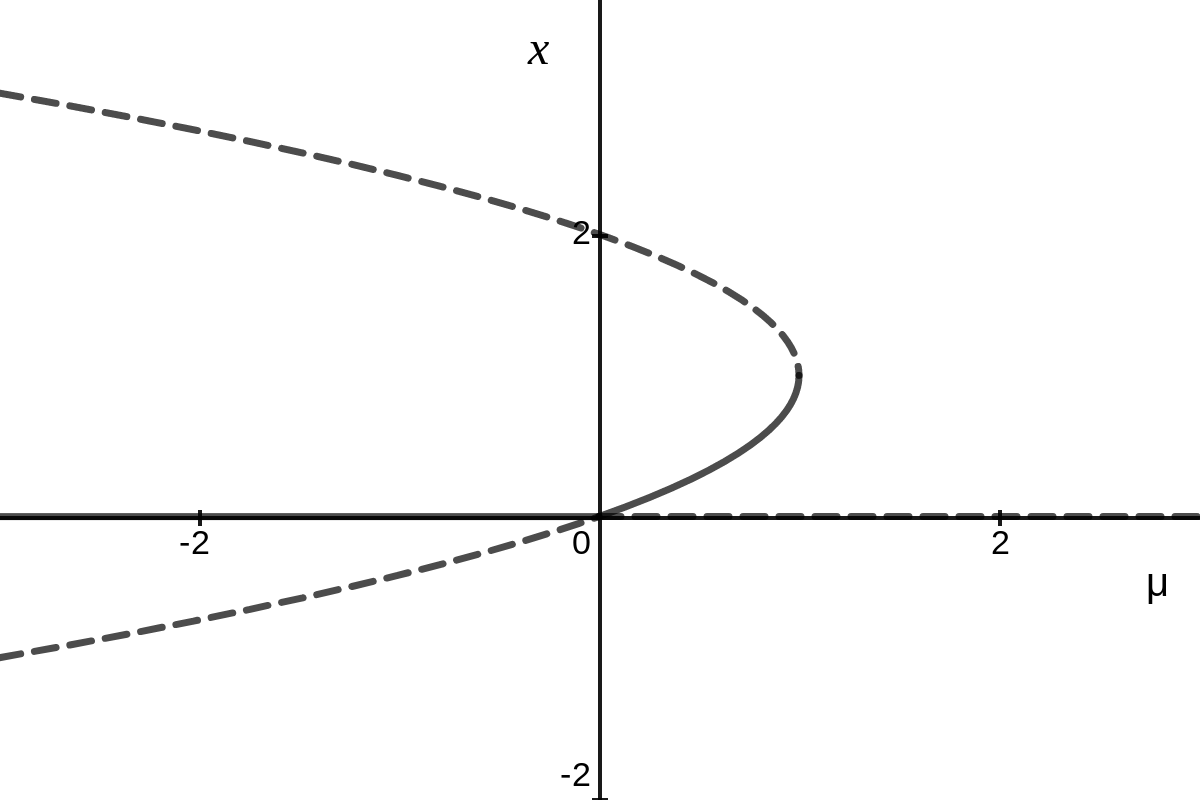
\includegraphics[height=0.3\textwidth]{img/2016S1.png}
    \end{center}
\end{enumerate}

\item \begin{qbox}
\begin{itemize}
    \item[\textbf{(a)}] Show that the second order ODE
    \[
    \frac{d^2x}{dt^2} + \left(\frac{dx}{dt}\right)^2 + x = 0
    \]
    can be put in the Hamiltonian form
    \[
    \frac{dx}{dt} = \pp{H}{p}, \qquad \frac{dp}{dt} = - \pp{H}{x}
    \]
    by defining
    \[
    p = e^{2x} \frac{dx}{dt}.
    \]
    What is $H(x,p)$?
    \item[\textbf{(b)}] Sketch the phase plane of the resulting Hamiltonian system.
\end{itemize}
\end{qbox}
\begin{enumerate}
    \item Our definition of $p$ immediately gives $\dot x = pe^{-2x}$. We now solve for $\dot p:$
    \begin{align*}
        \dot p &= 2e^{2x}\dot x^2 + e^{2x}\ddot x
        \\
        &= 2e^{2x}\dot x^2 + e^{2x}(-\dot x^2 - x) \\
        &= e^{2x}\dot x^2 - xe^{2x} \\
        &= e^{2x}\left(pe^{-2x}\right)^2 - xe^{2x} \\
        &= p^2 e^{-2x} - xe^{2x}
    \end{align*}
    Integrating up to find $H$, we have
    \begin{align*}
    \dot x = \pp{H}{p} \so H &= \frac{1}{2}p^2e^{-2x} + f(x)
    \\
    -\dot p = \pp{H}{x} \so H &= \frac{1}{2}p^2e^{-2x} + \int xe^{2x}\,dx + g(p) = \frac{1}{2}p^2e^{-2x} + \frac{1}{2}xe^{2x} - \frac{1}{4} e^{2x} + g(p)
    \end{align*}
    So, matching $f(x)$ and $g(p)$, we get
    \[
    H(x, p) = \frac{1}{2}p^2e^{-2x} + \frac{1}{2}xe^{2x} - \frac{1}{4} e^{2x}
    \]
    
    \item Our system is given by
    \[
    \begin{cases}
    \dot x = pe^{-2x} \\
    \dot p = p^2e^{-2x} - xe^{2x}.
    \end{cases}
    \]
    The only point for which $\dot x = 0$ is $p = 0$, which then yields $x = 0$ for $\dot p = 0$. So, our only fixed point is $(x, p) = (0, 0)$. We examine the flow along the coordinate axes, as well: when $x = 0$, we get $\dot x = p$ and $\dot p = p^2$, and when $p = 0$, we get $\dot x = 0$ and $\dot p = -xe^{2x}$. This produces the following flow:
    
    \begin{center}
    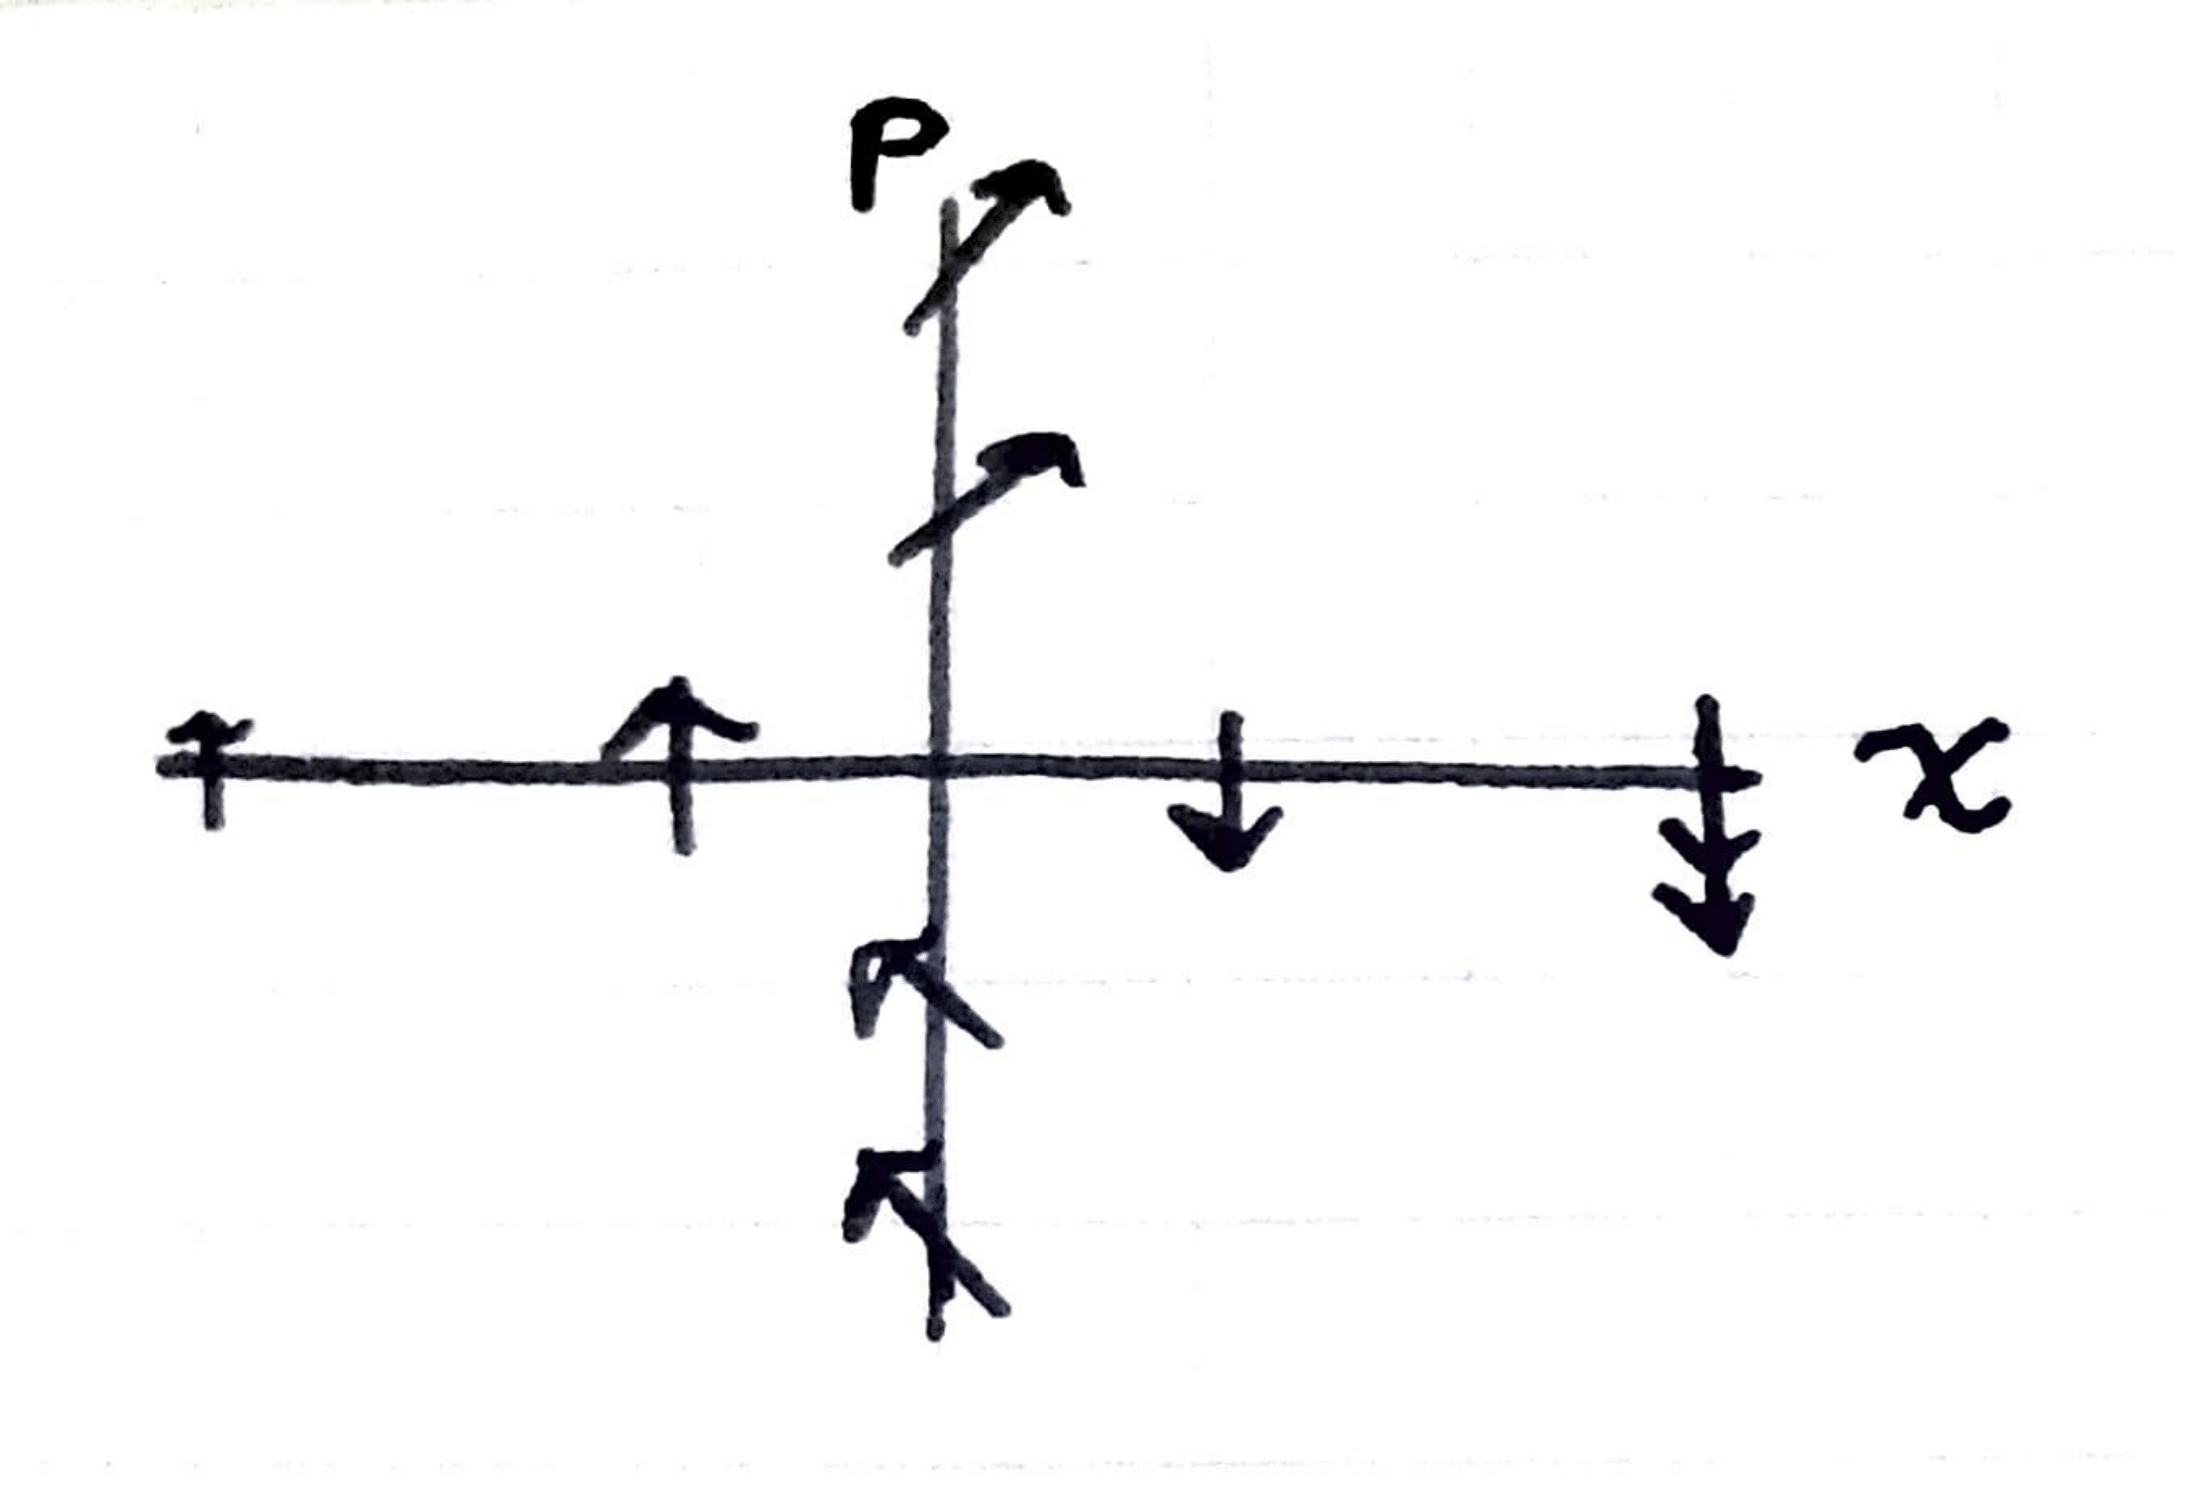
\includegraphics[height=0.3\textwidth]{img/2016S2b1.png}
    \end{center}
    
    Which yields the following phase plane:
    
    \begin{center}
    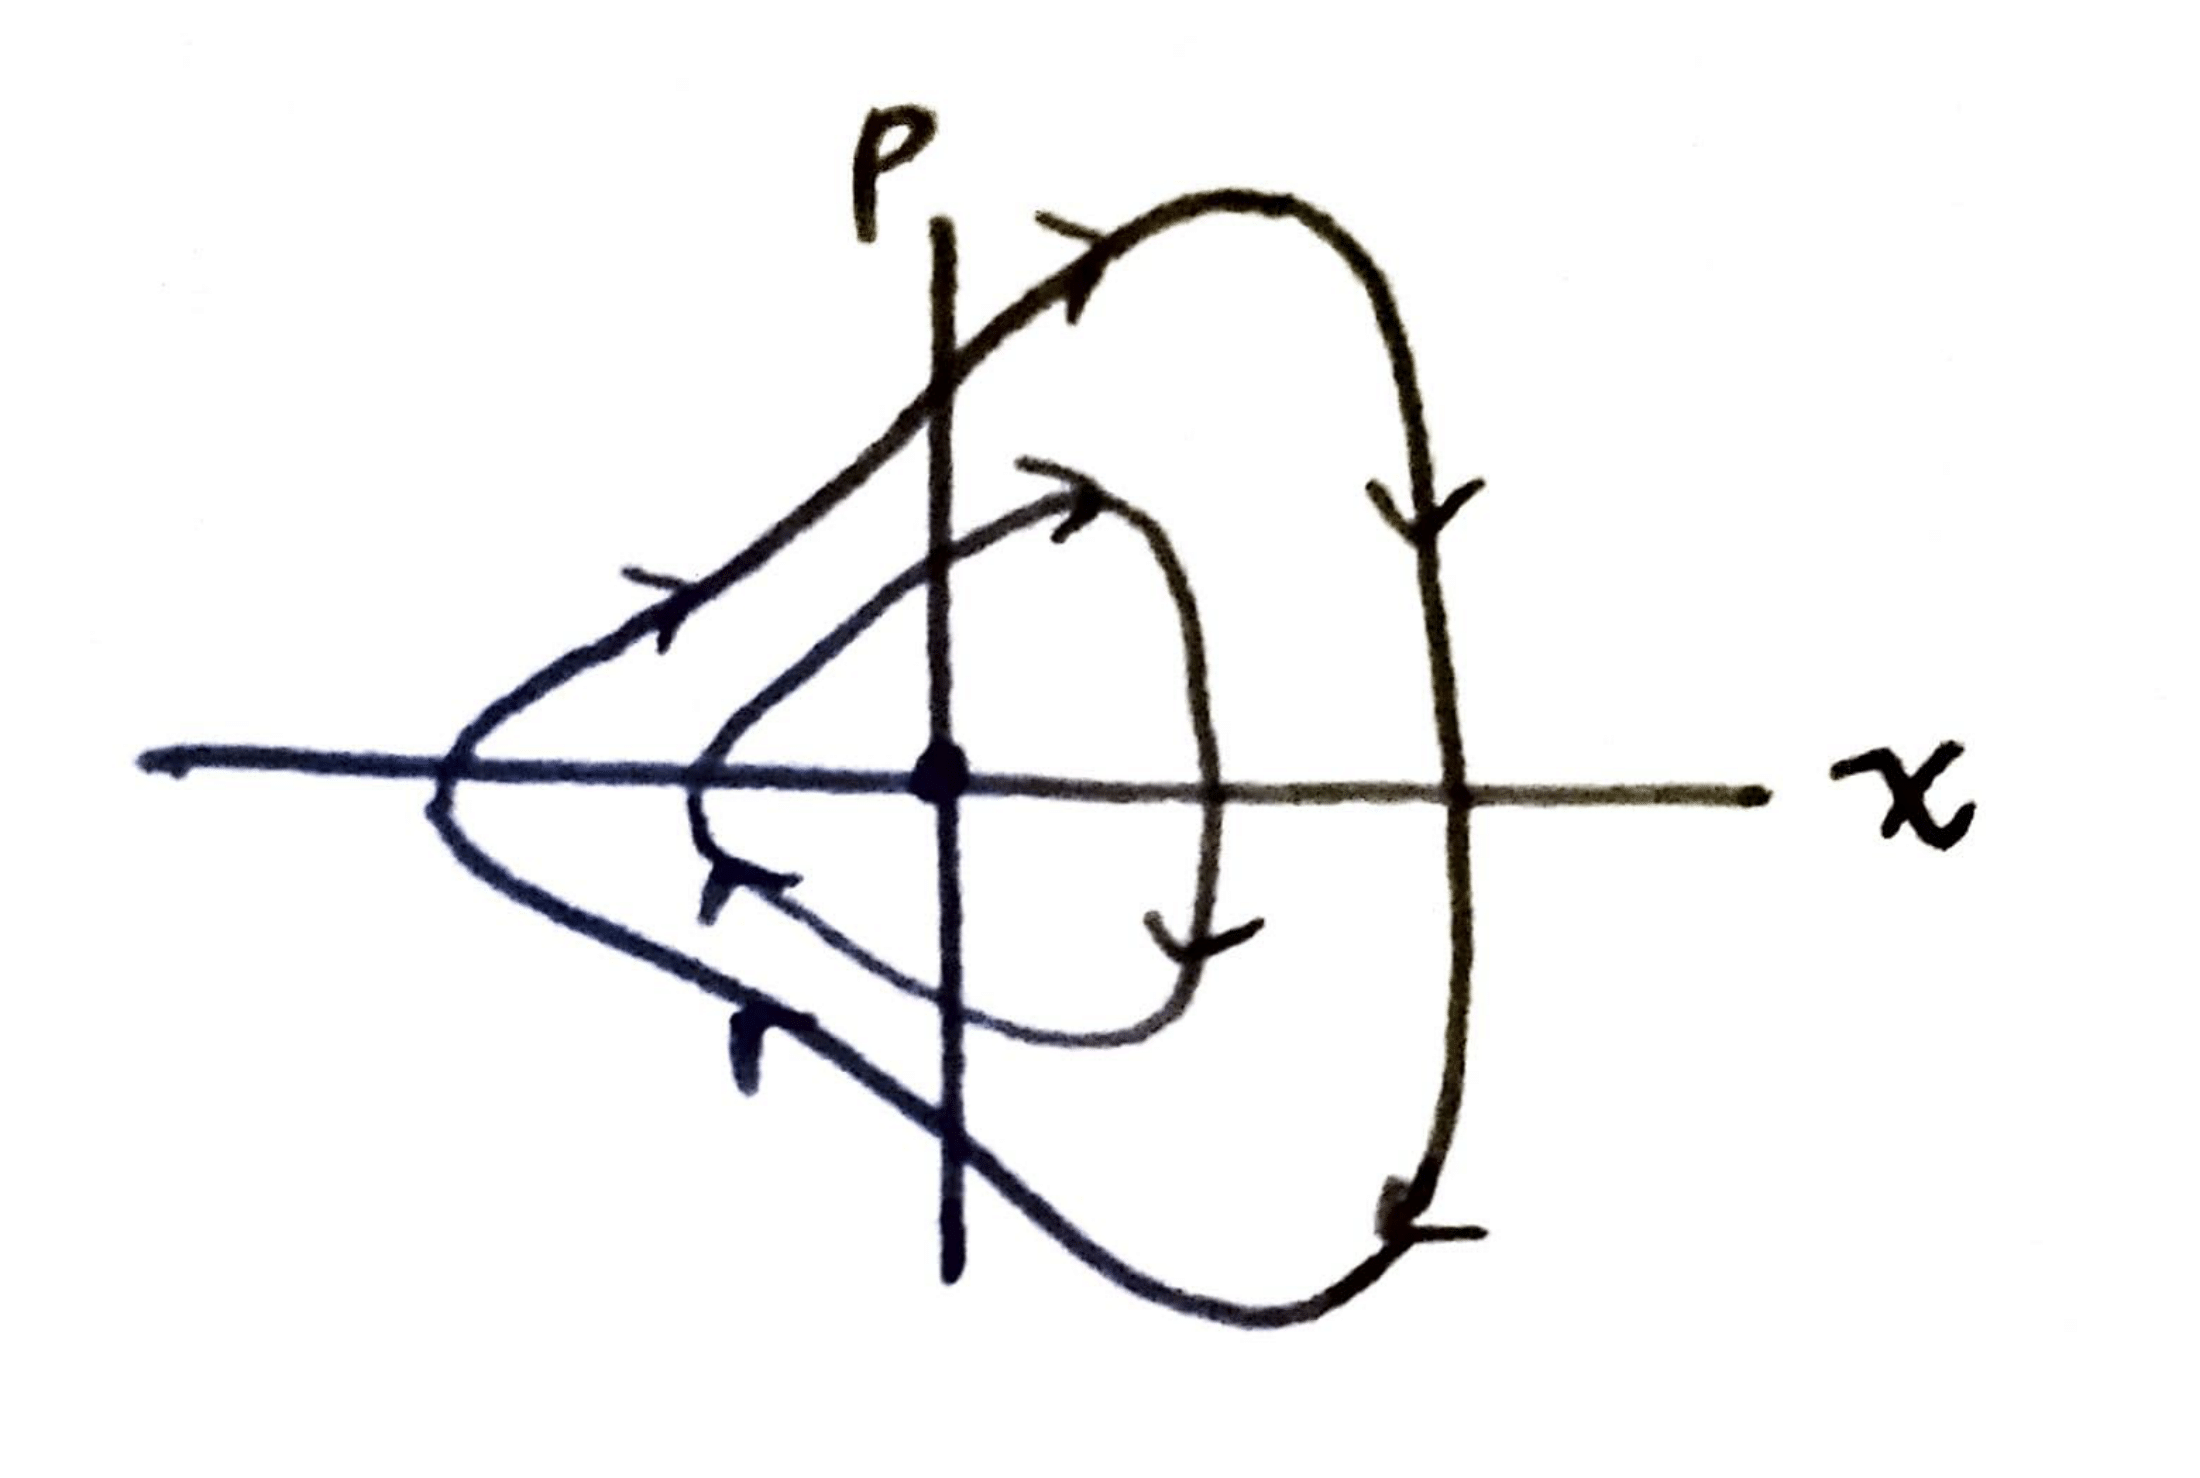
\includegraphics[height=0.3\textwidth]{img/2016S2b2.png}
    \end{center}
\end{enumerate}

\item \begin{qbox}
Suppose a perfectly flexible rope of length $2a$ with uniform density $\rho$ hangs under gravity from two fixed points $(-b, 0)$ and $(b, 0)$ in the $x y$-plane where $b < a$ and the gravity points downward (i.e., the negative $y$ direction). Find the shape of this rope, $y = y(x)$, that
minimizes the potential energy
\[
V = \rho g \int_{-b}^b y \sqrt{ 1 + y'^2}\,dx
\]
\textit{Hint:} The constraint is of course the arc length of the rope must be $2a$.
\end{qbox}
We assume the rope is symmetric. In this way, our arc length constraint is
\[
\int_0^b \sqrt{1 + y'^2}\,dx = a.
\]
We use a Lagrange multiplier, so that our goal is to minimize the integral of $h$, where
\[
h = (y + \lambda)\sqrt{1 + y'^2}.
\]
The Euler-Lagrange equation is
\[
\pp{h}{y} = \frac{d}{dx}\pp{h}{y'}.
\]
However, since $h$ is not explicitly dependent on $x$, we can use the simpler form
\[
h - y'\pp{h}{y'} = c,
\]
where $c$ is some constant. We compute $\partial h/\partial y':$
\begin{align*}
    \pp{h}{y'} &= \frac{(y + \lambda)y'}{\sqrt{1 + y'^2}}
\end{align*}
So, our Euler-Lagrange equation becomes
\begin{align*}
    (y + \lambda)\sqrt{1 + y'^2} - \frac{(y + \lambda)y'^2}{\sqrt{1 + y'^2}} &= c
    \\
    (y + \lambda)(1 + y'^2) - (y + \lambda)y'^2 &= c\sqrt{1 + y'^2}
    \\
    y + \lambda &= c\sqrt{1 + y'^2}
    \\
    (y + \lambda)^2 &= c^2(1 + y'^2)
    \\
    (y + \lambda)^2 - c^2 &= c^2y'^2
    \\
    \sqrt{(y + \lambda)^2 - c^2} &= cy'
    \\
    \frac{cy'}{\sqrt{(y + \lambda)^2 - c^2}} &= 1
    \\
    \int \frac{c\,dy}{\sqrt{(y + \lambda)^2 - c^2}} &= x + d
\end{align*}
We integrate the left-hand side:
\begin{align*}
    \int \frac{c\,dy}{\sqrt{(y + \lambda)^2 - c^2}}
    &=
    \int \frac{c\cdot c \sinh u\,du}{\sqrt{c^2\cosh^2 u - c^2}} &\left(\lambda + y = c\cosh u\right)
    \\
    &=
    \int \frac{c\sinh u\,du}{\sqrt{\cosh^2 u - 1}}
    \\
    &=
    \int \frac{c\sinh u\,du}{\sqrt{\sinh^2 u}}
    \\
    &=
    \int c\,du
    \\
    &= c u
    \\
    &= c \cdot \cosh^{-1}\left(\frac{\lambda + y}{c}\right)
\end{align*}
So, we now have
\begin{align*}
    c \cdot \cosh^{-1}\left(\frac{\lambda + y}{c}\right) &= x + d
    \\
    \cosh^{-1}\left(\frac{\lambda + y}{c}\right) &= \frac{x + d}{d}
    \\
    \frac{\lambda + y}{c} &= \cosh\left(\frac{x + d}{c}\right)
    \\
    y &= c\cdot \cosh\left(\frac{x + d}{c}\right) - \lambda
\end{align*}
Since we've assumed symmetry, we have $y'(0) = 0$, and so we get
\begin{align*}
    y'(0) = \sinh\left(\frac{0 + d}{c}\right) = 0 \so d = 0.
\end{align*}
So, now we have
\[
y = c\cdot \cosh\left(\frac{x}{c}\right) - \lambda.
\]
The boundary condition $y(b) = 0$ gives
\begin{align*}
    c\cdot \cosh\left(\frac{b}{c}\right) = \lambda,
\end{align*}
and so we have
\[
y = c\left[ \cosh\left(\frac{x}{c}\right) - \cosh\left(\frac{b}{c}\right)\right].
\]
Finally, we find $c$ via our arc length constraint:
\begin{align*}
    a &= \int_0^b \sqrt{1 + y'^2}\,dx
    \\
    &= \int_0^b \sqrt{1 + \sinh^2(x/c)}\,dx
    \\
    &= \int_0^b \cosh\left(\frac{x}{c}\right)\,dx
    \\
    &=
    c\sinh\left(\frac{b}{c}\right)
\end{align*}
So, we end with
\[
y = c\left[ \cosh\left(\frac{x}{c}\right) - \cosh\left(\frac{b}{c}\right)\right],
\]
where $c$ is the constant such that
\[
c\sinh\left(\frac{b}{c}\right) = a.
\]

\item \begin{qbox}
Let $f(\theta)$ be the $2\pi$-periodic function such that $f(\theta) = e^\theta$ for $-\pi < \theta \leq \pi$, and let $\sum_{n = -\infty}^\infty c_n e^{in\theta}$ be its Fourier series; thus 
\[
e^\theta = \sum_{n = -\infty}^\infty c_ne^{in\theta}
\]
for $\abs \theta < \pi$.
\begin{itemize}
    \item[\textbf{(a)}] Compute $c_n, n \in \Z$, explicitly.
    
    \item[\textbf{(b)}] If we formally differentiate this equation, we obtain
    \[
    \displaystyle{e^\theta = \sum_{n = -\infty}^\infty c_nine^{in\theta}}.
    \]
    But then, $c_n = inc_n$ or $(1-in)c_n = 0$, so $c_n = 0$ for all $n$. This is obviously wrong; where is the mistake?
\end{itemize}
\end{qbox}

\begin{enumerate}
    \item Our coefficients are given by
    \begin{align*}
        c_n &= \frac{1}{2\pi} \int_{-\pi}^\pi e^\theta e^{-in\theta}\,d\theta
        % \\
        % &= \frac{1}{2\pi} \int_{-\pi}^\pi e^{(1-in)\theta}\,d\theta
        \\
        &= \frac{1}{2\pi} \frac{1}{(1 - in)} e^{(1-in)\theta}\bigg\vert_{-\pi}^\pi
        % \\
        % &= \frac{1}{2\pi} \frac{1}{(1 - in)} \left(e^{(1-in)\pi} - e^{(in-1)\pi}\right)
        \\
        &= \frac{1}{2\pi} \frac{1}{(1 - in)} \left(e^\pi(-1)^n - (-1)^ne^{-\pi}\right)
        \\
        &= \frac{(-1)^n}{2\pi(1 - in)} \left(e^\pi - e^{-\pi}\right).
    \end{align*}
    
    \item Since $f$ is only piecewise continuous, but not continuous, as its endpoints do not match, the derivative of its Fourier series does not give the Fourier series of its derivative.
\end{enumerate}

\item \begin{qbox}
Find a one-term approximation, that is valid for long time scales, of the solution to the following differential equation
\[
\epsilon\frac{d^2x}{dt^2} + \epsilon\frac{dx}{dt} + x = \cos t
\]
for $t > 0$, with initial conditions $x(0) = 0$ and $dx/dt\big\vert_{t=0}=0$.
\begin{center}
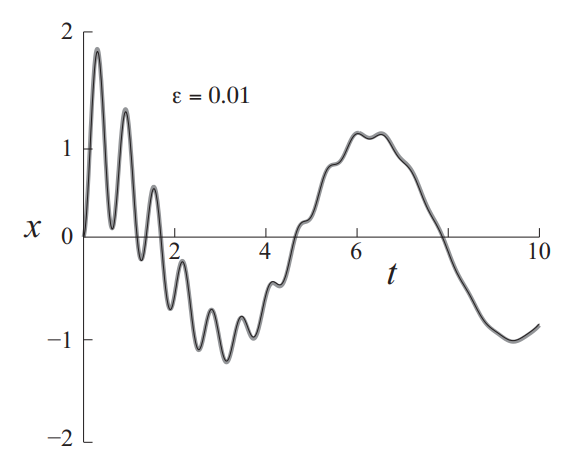
\includegraphics[height=0.4\textwidth]{img/2016S5.png}
\end{center}
Figure 1: This is a numerical solution of the equation with $\epsilon = 0.01$ (gray), plotted with my solution for the one term approximation, valid for long time scales (black).
\end{qbox}
We let $t_1 = t$ and $t_2 = \epsilon^\alpha t$. Then, our equation becomes
\begin{align*}
\epsilon\left(\partial_{t_1}^2 + 2\epsilon^\alpha \partial_{t_1t_2} + \epsilon^{2\alpha}\partial_{t_2}^2\right)x + \epsilon\left(\partial_{t_1} + \epsilon^{\alpha}\partial_{t_2}\right)x + x &= \cos t_1
\\
\big(\undernum{\epsilon\partial_{t_1}^2}{1} + \undernum{2\epsilon^{1 + \alpha} \partial_{t_1t_2}}{2} + \undernum{\epsilon^{1 + 2\alpha}\partial_{t_2}^2}{3}\big)x + \left(\epsilon\partial_{t_1} + \epsilon^{1 + \alpha}\partial_{t_2}\right)x + \undernum{x}{4} &= \cos t_1
\end{align*}
The natural choice is $\circled 3 \thicksim \circled 4$, which yields $\alpha = -1/2$. This indeed results in $\circled 3$ and $\circled 4$ being of leading order. So, we now have
\begin{align*}
\left(\epsilon\partial_{t_1}^2 + 2\epsilon^{1/2} \partial_{t_1t_2} + \partial_{t_2}^2\right)x + \left(\epsilon\partial_{t_1} + \epsilon^{1/2}\partial_{t_2}\right)x + x &= \cos t_1
\end{align*}
Our leading-order expression is $\Ord{1}:$
\begin{align*}
    \partial^2_{t_2}x_0 + x_0 &= \cos t_1
    \\
    x_0 &= \cos t_1 + A(t_1)\sin(t_2) + B(t_1)\cos(t_2).
\end{align*}
Now, we look to our initial conditions. $x_0(0, 0) = 0$ yields
\[
0 = 1 + B(0) \so B(0) = -1,
\]
while our other initial condition becomes $\left(\partial_{t_1} + \epsilon^{-1/2}\partial_{t_2}\right)x\big\vert_{0,0} = 0$. The leading-order expression from this term is thus $\partial_{t_2}x\big\vert_{0, 0} = 0$, and so we get
\begin{align*}
    \partial_{t_2}x = A(t_1)\cos(t_2) - B(t_1)\sin(t_2)
    \so A(0) = 0.
\end{align*}
Next, we take $x \thicksim x_0 + \epsilon^{1/2}x_1$ and look at our $\Ord{\epsilon^{1/2}}$ expression:
\begin{align*}
    \partial_{t_2}^2 x_1 + 2\partial_{t_1t_2}x_0 + \partial_{t_2}x_0 + x_1 = 0
\end{align*}
In order to eliminate secular terms, we want to set $2\partial_{t_1t_2}x_0 + \partial_{t_2}x_0 = 0$. We examine this term:
\begin{align*}
    2\partial_{t_1t_2}x_0 + \partial_{t_2}x_0
    &=
    2A'(t_1)\cos(t_2) - 2B'(t_1)\sin(t_2) + A(t_1)\cos(t_2) - B(t_1)\sin(t_2)
\end{align*}
So, grouping sines and cosines, we want $2A'(t_1) + A(t_1) = 0$ and $2B'(t_1) + B(t_1) = 0$. This yields
\[
A(t_1) = k_1e^{-t_1/2}, \qquad B(t_1) = k_2e^{-t_1/2}.
\]
Our initial conditions yield $k_1 = 0$ and $k_2 = -1$, and so we finally end up with
\begin{align*}
    x_0 &= \cos(t_1) - e^{-t_1/2}\cos(t_2)
    \\
    &\Downarrow \\
    x_0 &= \cos(t) - e^{-t/2}\cos\left(\epsilon^{-1/2}t\right).
\end{align*}

\item
\begin{qbox}
Friedrichs' (1942) model problem for a boundary layer in a viscous fluid is
\[
\epsilon\frac{d^2y}{dx^2} = a - \frac{dy}{dx}
\]
for $0 < x < 1$ and $y(0) = 0$, $y(1) = 1$, and $a$ is a given positive constant. After finding the first term of the inner and outer expansions, derive a composite expansion for the solution to this problem.
\end{qbox}

Our leading-order outer equation is
\[
0 = a - y' \so y_{out} = ax + C.
\]
We can fit either boundary condition with this constant, so for now, we leave $C$ general. Next, for the boundary layer, we rescale $x$ as $\hat x = (x - x_B)/\epsilon^\alpha:$
\begin{align*}
    \undernum{\epsilon^{1 - 2\alpha}y''}{1} + \undernum{\epsilon^{-\alpha}y'}{2} - \undernum{a}{3} &= 0
\end{align*}
Matching $\circled 1 \thicksim \circled 2$ gives $\alpha = 1$, which appears to be a reasonable expansion. Then our equation becomes
\[
\frac{1}{\epsilon} y'' + \frac{1}{\epsilon} y' - a = 0.
\]
The leading-order equation is
\begin{align*}
    y'' + y' &= 0
    \\
    y'' &= -y' \\
    y' &= Ae^{-\hat x} \\
    y_{in} &= -Ae^{-\hat x} + B
\end{align*}
If we take $\hat x \to \infty$, then $y_{in}$ approaches the value $B$. If, on the other hand, we were to take $\hat x \to -\infty$, then $y_{in}$ would be unbounded. So, we deduce that the boundary layer occurs at $x = 0$ in order for our limits to make sense. Solving $y_{in}(0) = 0$ yields
\[
0 = -A + B \so y_{in} = A\left(1 - e^{-\hat x}\right),
\]
and solving $y_{out}(1) = 1$ yields
\[
1 = a + C \so y_{out} = ax + 1 - a.
\]
Now, we match.
\begin{align*}
    \lim_{\hat x \to \infty} y_{in} = A, \qquad \lim_{x \to 0} y_{out} = 1 - a
\end{align*}
So, we have $A = 1 - a = y_{overlap}$, and so our final solution is
\begin{align*}
    y &\thicksim y_{in} + y_{out} - y_{overlap} 
    = 
    (1 - a)\left(1 - e^{-x/\epsilon}\right) + ax
\end{align*}

\end{enumerate}

\chapter*{Fall 2015}
\chaptermark{Fall 2015}
\addcontentsline{toc}{chapter}{Fall 2015}

\begin{enumerate}
\item \begin{qbox}
Consider the system
\begin{align*}
    \dot x &= -y - x^3 \\
    \dot y &= x^5.
\end{align*}
\begin{itemize}
    \item[\textbf{(a)}] Is the equilibrium $(x, y) = (0, 0)$: (i) linearly stable; (ii) linearly asymptotically stable; (iii) hyperbolic? What do your answers imply about the nonlinear stability of the equilibrium?
    
    \item[\textbf{(b)}] Find a Liapunov function for the system of the form
    \[
    V (x, y) = Ax^6 +B y^2.
    \]
    What can you conclude about the nonlinear stability of $(0, 0)$ from the Liapunov function?
\end{itemize}
\end{qbox}

\begin{enumerate}
    \item We compute the Jacobian of our system at the point $(0, 0):$
    \begin{align*}
        J &= \mtx{rr}{-3x^2 & -1 \\ 5x^4 & 0} \so
        J\big\vert_{0,0} = \mtx{rr}{0 & -1 \\ 0 & 0} \so \lambda = 0, 0.
    \end{align*}
    Since both of our eigenvalues are zero, we have that this equilibrium is linearly stable, but not linearly asymptotically stable and not hyperbolic. Since linear stability analysis fails here, we do not know anything about the nonlinear stability of the equilibrium.
    
    \item We compute $dV/dt:$
    \begin{align*}
        \frac{dV}{dt} &= 6Ax^5 \dot x + 2By \dot y \\
        &= 6Ax^5\left(-y - x^3\right) + 2Byx^5 \\
        &= -6Ax^8 + (2B - 6A)yx^5
    \end{align*}
    We set $2B = 6A$ and $A > 0$. For simplicity, we choose $A = 1$. This yields
    \begin{align*}
        \frac{dV}{dt} = -6x^8 \leq 0 \textrm{ for all }x, y \in \R.
    \end{align*}
    So, we have that $V(x, y) = x^6 + 3y^2$ decreases or remains constant along trajectories, and $V(0, 0) = 0$ but is positive elsewhere. So, we have a Liapunov function (though not a strict one, as $dV/dt\big\vert_{x = 0} = 0$ for any choice of $y \in \R$), and so our fixed point is Liapunov stable but not asymptotically stable.
\end{enumerate}

\item\begin{qbox}
Consider the discrete dynamical system with iterates $x_n$ given by the map
\[
x_{n+1} = -\mu x_n - x_n^3,
\]
where $\mu$ is a real parameter.
\begin{itemize}
    \item[\textbf{(a)}] Find the fixed points of the system as a function of $\mu$ and determine their linearized stability.
    \item[\textbf{(b)}] What kind of bifurcation occurs at $x_n = 0$ as $\mu$ increases through $\mu = 1$?
    \item[\textbf{(c)}] If $x_n$ is small and $\mu = 1+\epsilon$ is close to 1, show that
    \[
    x_{n+2} \approx (1+2\epsilon)x_n + 2x_n^3
    \]
    after neglecting smaller terms. Determine whether the bifurcation in (b) is subcritical or supercritical.
\end{itemize}
\end{qbox}

\begin{enumerate}
    \item To find the fixed points, we set $x_{n+1} = x_n:$
    \begin{align*}
        \bar x &= -\mu \bar x - \bar x^3 \\
        0 &= (1+\mu)\bar x + \bar x^3 \\
        0 &= \bar x\left(1 + \mu + \bar x^2\right) \\
        \bar x &= 0,\ \pm\sqrt{-1-\mu}
    \end{align*}
    Note that the second pair of fixed points only exists for $\mu < -1$. Now, to find their stability, we compute $f'(\bar x)$ for each point:
    \begin{align*}
        f'(\bar x) &= -\mu - 3\bar x^2 \\ 
        &\Downarrow \\
        f'(0) &= - \mu \\
        f'\left(\pm\sqrt{-1 - \mu}\right) &= -\mu + 3(1 + \mu)
        =
        2\mu + 3
    \end{align*}
    So, we have that
    \begin{align*}
        \bar x = 0 \textrm{ is }&\begin{cases}
        \textrm{unstable}&: \mu < -1 \\
        \textrm{stable} &: \mu \in (-1, 1) \\
        \textrm{unstable}&: \mu > 1
        \end{cases} \\
        \bar x = \pm \sqrt{-1-\mu} \textrm{ are both }&\begin{cases}
        \textrm{unstable}&: \mu < -2 \\
        \textrm{stable} &: \mu \in (-2, -1)
        \end{cases}
    \end{align*}
    \item As $\mu$ increases through $\mu = 1$, $\bar x = 0$ moves from being stable to unstable. Its eigenvalue is passing through $\lambda = -1$, and there are no other fixed points around this region for it to interact with, so we have a period-doubling bifurcation.
    
    \item If $x_n$ is small (we'll say $0 < x_n < 1$) and $\mu = 1 + \epsilon$ is close to 1, then we compute $x_{n+2}:$
    \begin{align*}
        x_{n+2} &= -\mu x_{n+1} - x_{n+1}^3 \\
        &= \mu(\mu x_n + x_n^3) + (\mu x_n + x_n^3)^3 \\
        &= \mu^2 x_n + \mu x_n^3 + \mu^3 x_n^3 + 3\mu^2x_n^5 + 3\mu x_n^7 + x_n^9 \\
        &= (1 + 2\epsilon + \epsilon^2) x_n + (1 + \epsilon) x_n^3 + (1 + 3\epsilon + 3\epsilon^2 + \epsilon^3) x_n^3 + \Ord{x_n^5} \\
        &\approx (1+2\epsilon)x_n +2x_n^3.
    \end{align*}
    This value is larger than $x_n$, even though the terms $x_n$ are small. As $x_n$ grows larger, these additional terms compound, rather than dying off, so there is no stable orbit which we are converging to. Therefore, we have a subcritical period-doubling bifurcation.
\end{enumerate}

\item \begin{qbox}
Find among all continuous curves of length $\ell$ in the upper half-plane of $\R^2$ passing through $(-a, 0)$ and $(a, 0)$, the one that, together with the interval $[-a,a]$, encloses the largest area. Then, compute the maximum area too.

\textit{Hint:} You may want to use the \textit{symmetry} of the problem to your advantage! Also, note that the length of the curve $\ell$ does not include the length of the interval $2a$ on the horizontal axis.
\end{qbox}

Our goal is to minimize the following functional:
\[
2\int_{0}^af(x)\,dx
\]
subject to the following constraints:
\[
2\int_0^a \sqrt{1 + f'^2}\,dx = \ell, \quad f'(0) = 0,\quad f(a) = 0.
\]
Using the method of Lagrange Multipliers, we set
\[
h = f + \lambda \sqrt{1 + f'^2}
\]
and use the Euler-Lagrange equation
\[
\pp{h}{f} = \frac{d}{dx}\left[\pp{h}{f'}\right].
\]
Computing these terms, we get
\begin{align*}
    1 &= \frac{d}{dx}\left[\frac{\lambda f'}{\sqrt{1 + f'^2}}\right] \\
    x + c &= \frac{\lambda f'}{\sqrt{1 + f'^2}}
\end{align*}
Plugging in the condition $f'(0) = 0$, we get $c = 0$. So, we now have
\begin{align*}
    x &= \frac{\lambda f'}{\sqrt{1 + f'^2}} \\
    x\sqrt{1 + f'^2} &= \lambda f' \\
    x^2\left(1 + f'^2\right) &= \lambda^2 f'^2 \\
    x^2 &= \left(\lambda^2 - x^2\right)f'^2 \\
    f'^2 &= \frac{x^2}{\lambda^2 - x^2} \\
    f' &= \pm \frac{x}{\sqrt{\lambda^2 - x^2}}
\end{align*}
As $f \geq 0$ for $x > 0$ and as $f(a) = 0$, we know that $f$ must be concave-down rather than concave-up , and so we choose the $(-)$ from the $(\pm)$. Now, we have
\begin{align*}
    f' &= - \frac{x}{\sqrt{\lambda^2 - x^2}} \\
    f &= - \int \frac{x}{\sqrt{\lambda^2 - x^2}} \,dx \\
    f &= \frac{1}{2}\int u^{-1/2}\,du &(u = \lambda^2 - x^2,\ du = -2xdx) \\
    f &= u^{1/2} + C \\
    f &= \sqrt{\lambda^2 - x^2} + C
\end{align*}
The boundary condition $f(a) = 0$ yields
\begin{align*}
    C &= - \sqrt{\lambda^2 - a^2} \so f(x) = \sqrt{\lambda^2 - x^2}- \sqrt{\lambda^2 - a^2}.
\end{align*}
Now, we solve for $\lambda:$
\begin{align*}
    \ell &= 2\int_0^a \sqrt{1 + f'^2}\,dx \\
    &= 2\int_0^a \sqrt{1 + \frac{x^2}{\lambda^2 - x^2}}\,dx \\
    &= 2\int_0^a \sqrt{\frac{\lambda^2}{\lambda^2 - x^2}}\,dx\\
    &= 2\lambda \int_0^a \frac{1}{\sqrt{\lambda^2 - x^2}}\,dx \\
    &= 2\lambda \int_0^{\arcsin(a/\lambda)}\,du &(x = \lambda \sin u,\ dx = \lambda\cos u\,du) \\
    &= 2\lambda\arcsin\left(\frac{a}{\lambda}\right)
\end{align*}
So, $\lambda$ is the value such that
\[
2\lambda\arcsin\left(\frac{a}{\lambda}\right) = \ell.
\]
Finally, we compute the maximum area:
\begin{align*}
    2\int_0^a f(x)\,dx 
    &= 
    2\int_0^a \left(\sqrt{\lambda^2 - x^2}- \sqrt{\lambda^2 - a^2}\right)\,dx \\
    &=
    -2a\sqrt{\lambda^2 - a^2} + 2\int_0^a\sqrt{\lambda^2 - x^2}\,dx \\
    &= -2a\sqrt{\lambda^2 - a^2} + 2\int_0^{\arcsin(a/\lambda)}\lambda^2\cos^2 u \,du &(x = \lambda \sin u) \\
    &= -2a\sqrt{\lambda^2 - a^2} + \lambda^2\int_0^{\ell/2\lambda}(\cos(2u) + 1) \,du
    \\
    &= -2a\sqrt{\lambda^2 - a^2} + \lambda^2\left[\frac{1}{2}\sin(2u) + u\right]_0^{\ell/2\lambda}
    \\
    &= -2a\sqrt{\lambda^2 - a^2} + \lambda^2\left[\frac{1}{2}\sin\left(\frac{\ell}{\lambda}\right) + \frac{\ell}{2\lambda}\right]
    \\
    &= -2a\sqrt{\lambda^2 - a^2} + \frac{\lambda^2}{2}\sin\left(\frac{\ell}{\lambda}\right) + \frac{\ell\lambda}{2},
\end{align*}
where $\lambda$ is given as above.

\item \begin{qbox}
Consider a simple rectangular domain $\Omega = \sett{(x, y) \in \R^2}{0 < x< a,\ 0 < y < b}$ with $a > b$, and the simple heat equation with the following initial and boundary conditions:
\[
\begin{cases}
\dfrac{\partial u}{\partial t} = \dfrac{\partial^2 u}{\partial x^2} + \dfrac{\partial^2 u}{\partial y^2} &\textrm{for } (x, y, t) \in \Omega \times [0, \infty);
\\
\dfrac{\partial u}{\partial x}(0, y, t) = \dfrac{\partial u}{\partial x}(a, y, t) = 0  &\textrm{on } 0 \leq y \leq b,\ t\in [0, \infty);
\\
\dfrac{\partial u}{\partial y}(x, 0, t) = \dfrac{\partial u}{\partial y}(x, b, t) = 0  &\textrm{on } 0 \leq x \leq a,\ t\in [0, \infty);
\\
u(x, y, 0) = f(x, y) &\textrm{on }(x, y) \in \Omega.
\end{cases}
\]
\begin{itemize}
    \item[\textbf{(a)}] Write down the general solution of this problem as a double Fourier series. [Hint: Use the separation of variables.]
    \item[\textbf{(b)}] Identify the spatial modes (i.e., Fourier basis functions involving only $(x, y)$ variables, not $t$) corresponding to the three lowest frequencies.
    \item[\textbf{(c)}] Determine the solution of the above initial and boundary value problem in the case of $f(x, y) \equiv c =$ a real-valued constant.
\end{itemize}
\end{qbox}

\begin{enumerate}
\item We assume $u$ can be written in the form $u(x, y, t) = X(x)Y(y)T(t)$. Then, our PDE can be rewritten as follows:
\begin{align*}
    u_t &= u_{xx} + u_{yy} \\
    XYT' &= X''YT + XY''T \\
    \frac{T'}{T} &= \frac{X''}{X} + \frac{Y''}{Y} = \lambda,
\end{align*}
where $\lambda \in \R$. So, we can then write
\begin{align*}
    \frac{X''}{X} = \lambda - \frac{Y''}{Y} = \mu,
\end{align*}
for some $\mu \in \R$. We examine our $X$-equation first and find the sign of $\mu$.
\begin{align*}
    X'' &= \mu X \\
    \int_0^a X'' X\,dt &= \int_0^a \mu X^2\,dt \\
    X'X\big\vert_0^a - \int_0^a (X')^2\,dt &= \mu \int_0^a X^2\,dt &\textrm{(IBP)}
    \\
    - \int_0^a (X')^2\,dt &= \mu \int_0^a X^2\,dt &\textrm{(boundary terms vanish)}
\end{align*}
So, $\mu$ must be negative, and so we rewrite $\mu$ as $-\mu^2$. We now have the equation
\begin{align*}
    X'' = -\mu X \so X &= A\sin(\mu x) + B\cos(\mu x) \\
    X' &= \mu\big[A\cos(\mu x) - B \sin(\mu x)\big].
\end{align*}
The boundary condition $X'(0) = 0$ yields $A = 0$, so we now have
\begin{align*}
    X = B\cos(\mu x), \qquad X' &= -\mu B \sin(\mu x)
\end{align*}
The boundary condition $X'(a) = 0$ yields $\sin(\mu a) = 0$, and so $\mu a = m\pi$ or $\mu = m\pi/a$, for $m \in \N$. Thus,
\[
X_m(x) = \cos\left(\frac{m \pi }{a} x\right), \qquad m \in \N.
\]
Turning to our $Y$-equation, we now have $Y''/Y = \lambda + \mu^2 = -\eta^2$, as the boundary conditions are analogous to those of $X$, where $\eta \in \R$. We now are left to solve the same problem as before, but with $a$ replaced by $b$, and so we get
\[
Y_n(y) = \cos\left(\frac{n \pi }{b} y\right), \qquad n \in \N.
\]
Finally, we are left to solve the $T$-equation:
\[
T' = \lambda T \so T' = -\left(\mu_m^2 + \eta_n^2\right)T \so T = C e^{-\left(\mu_m^2 + \eta_n^2\right)t}
\]
where
\[
\mu_m = \frac{m\pi}{a}, \quad \eta_n = \frac{n\pi}{b}.
\]
So, $u(x, y, t)$ has the form
\[
u(x, y, t) = \sum_{m = 0}^\infty\sum_{n = 0}^\infty C_{mn} \cos\left(\mu_m x\right) \cos\left(\eta_n y\right)e^{-\left(\mu_m^2 + \eta_n^2\right)t}.
\]
Now, we plug in our boundary condition $u(x, y, 0) = f(x, y):$
\begin{align*}
    \sum_{m = 0}^\infty\sum_{n = 0}^\infty C_{mn} \cos(\mu_m x)\cos(\eta_n y) = f(x, y).
\end{align*}
We can then solve for the coefficients $C_{mn}$ of this double Fourier series and plug back into the general solution given above.

\item The spatial modes corresponding to the three lowest frequencies are $m = n = 0$, then $m = 1, n = 0$ and $m = 0, n = 1$:
\begin{align*}
    1, \quad \cos\left(\frac{\pi}{a}x\right), \quad \cos\left(\frac{\pi}{b}y\right).
\end{align*}

\item If $f(x, y) = c$, then our constants are defined by
\begin{align*}
    \sum_{m = 0}^\infty\sum_{n = 0}^\infty C_{mn} \cos(\mu_m x)\cos(\eta_n y) = c.
\end{align*}
So, we have $C_{m,n} = c$ for $m, n = 0$ and zero otherwise. Thus, the solution is simply
\[
u(x, y, t) = c.
\]

\end{enumerate}
% \addtocounter{enumi}{1}

\item \begin{qbox}
Consider the following regular Sturm-Liouville problem (RSLP):
\begin{align*}
    \begin{cases}
    f'' + \omega^2 f = g, \qquad 0 \leq x \leq 1 \\
    f'(0) = 0 = f'(1),
    \end{cases}
\end{align*}
where $\omega > 0$ is not an integer multiple of $\pi$.
\begin{itemize}
\item[\textbf{(a)}] Find the Green's function for this RSLP.
\item[\textbf{(b)}] What happens if we try this with $\omega = 0$?
\end{itemize}
\end{qbox}

See Spring 2019 Problem 4 --- identical problem.

\item \begin{qbox}
Find a one-term approximation, valid to order $\epsilon$, of the solution to the following differential equation
\[
\epsilon\frac{d^2y}{dx^2} + y\left(\frac{dy}{dx} + 3\right) = 0
\]
for $0 < x < 1$, with boundary conditions $y(0) = -1$ and $y(1) = 1$. 

It might be useful to know that
\[
\int\frac{dx}{-0.5x^2+a} = \sqrt{\frac{2}{a}}\tanh^{-1}\left(x\sqrt{\frac{1}{2a}}\right) + b
\]
where $a$ is a positive constant and $b$ is a constant.

It also might be useful to know that $\tanh$ is an odd function and that $\lim_{x\to\infty} \tanh(x) = 1$ and $\lim_{x\to-\infty} \tanh(x) = -1$.
\begin{center}
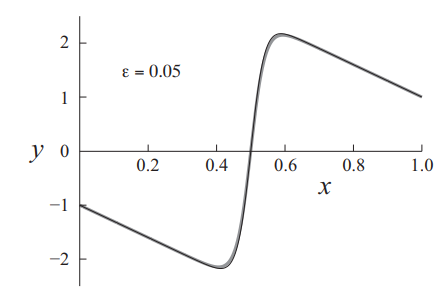
\includegraphics[height=0.3\textwidth]{img/2015F6.png}
\end{center}
Figure 1: This is a numerical solution of the equation with $\epsilon = 0.05$ (gray), plotted with my solution
for the one-term approximation (black).
\end{qbox}

We begin by computing the outer expansion, setting $\epsilon = 0:$
\[
y(y' +3) = 0 \so y' = -3 \so y = -3x + C
\]
Based on the image, we expect an interior layer. So, we use our boundary conditions to get the outer solution for the left and right sides:
\begin{align*}
    y(0) = -1 \so y_L &= -3x - 1 \\
    y(1) = 1\phantom{-} \so y_R &= -3x + 4
\end{align*}
Now, we compute our inner layer. We guess that the boundary will occur at $x = 0.5$, so we set $\hat x = (x - 0.5)/\epsilon^\alpha$. Now, our equation becomes
\begin{align*}
    \undernum{\epsilon^{1-2\alpha} y''}{1} + \undernum{\epsilon^{-\alpha}yy'}{2} + \undernum{3y}{3} &= 0
\end{align*}
Matching $\circled 1 \thicksim \circled 2$ yields $\alpha = 1$. So, our leading-order equation is $y'' + yy' = 0$, which becomes
\begin{align*}
    \frac{d^2 y}{d\hat x^2} &= -y \frac{dy}{d\hat x} \\
    \int \frac{d^2 y}{d\hat x^2}\,d\hat x &= -\int y\,dy \\
    y' &= -\frac{1}{2}y^2 + A
\end{align*}
Dividing out and integrating, using the given hint, we get
\begin{align*}
    \hat x + B &= \int\frac{dy}{-0.5y^2 + A}\\
    \hat x + B &= \sqrt{\frac{2}{A}}\tanh^{-1}\left(y\frac{1}{\sqrt{2A}}\right) \\
    \hat x \sqrt{\frac{A}{2}} + B 
    &= \tanh^{-1}\left(y\frac{1}{\sqrt{2A}}\right) \\
    \tanh\left(\hat x \sqrt{\frac{A}{2}} + B\right) &= \frac{y}{\sqrt{2A}} \\
    y(\hat x) &= \sqrt{2A}\tanh\left(\hat x \sqrt{\frac{A}{2}} + B\right)
\end{align*}
Since we want $y_{in} = 0$ at $\hat x = 0$, we set $B = 0$. So, our expression is now
\[
y_{in} = \sqrt{2A}\tanh\left(\hat x \sqrt{\frac{A}{2}}\right)
\]
Lastly, we want to match our inner and outer solutions as we move out of the boundary.
\begin{align*}
    \lim_{x \to 0.5}y_L &= -\frac{5}{2} &\quad \lim_{x \to 0.5}y_R &= \frac{5}{2}\\
    \lim_{\hat x \to -\infty} y_{in} &= -\sqrt{2A} &\quad \lim_{\hat x \to \infty} y_{in} &= \sqrt{2A}
\end{align*}
So, we require $\sqrt{2A} = 5/2$. Our overlap in the left region is thus $-5/2$ and our overlap in the right region is $5/2$. So, our inner solution becomes
\[
y_{in} = \frac{5}{2}\tanh\left(\frac{5}{4}\hat x\right)
\]
Note that our overlap in the left region is thus $-5/2$ and our overlap in the right region is $5/2$. Moreover, $y_L + 5/2 = y_R - 5/2 = -3x + 3/2$, and so our outer solutions combine into one expression and we get the composite solution
\begin{align*}
    y(x) = -3x + \frac{3}{2} + \frac{5}{2}\tanh\left(\frac{5(x - 1/2)}{4\epsilon}\right).
\end{align*}

\end{enumerate}

\chapter*{Spring 2015}
\chaptermark{Spring 2015}
\addcontentsline{toc}{chapter}{Spring 2015}

\begin{enumerate}
\item \begin{qbox}
Consider the following two sets of coupled ODEs.

Set 1 (Eqs. 1):
\begin{align*}
    \frac{dx}{dt} &= -y - x\left(x^2 + y^2\right) \\
    \frac{dy}{dt} &= x - y \left(x^2 + y^2\right)
\end{align*}
Set 2 (Eqs. 2):
\begin{align*}
    \frac{dx}{dt} &= -y + xy^2 \\
    \frac{dy}{dt} &= x - x^2 y
\end{align*}
\begin{itemize}
    \item Show that, for both sets of ODEs, linear stability predicts that the fixed point $(x = 0, y = 0)$ is a center.
    
    \item For one set of ODEs, the fixed point $(x = 0, y = 0)$ is, in fact, a stable spiral. Which one? Is it possible for the linearized equations to correctly predict the stability of the fixed-point? Why or why not?
    
    \item For one set of ODEs, the fixed point $(x = 0, y = 0)$ is, in fact, a center. Which one? Show that, for this set of ODEs, closed orbits exist.
\end{itemize}
\end{qbox}

We examine the Jacobian of each set of equations:
\begin{alignat*}{3}
    J^{(1)} &= \mtx{cc}{-3x^2 - y^2 & -1 - 2xy \\ 1 - 2xy & -x^2 - 3y^2} \andso J^{(1)}\big\vert_{0,0} &= \mtx{cr}{0 & -1 \\ 1 & 0}
    \\
    J^{(2)} &= \mtx{cc}{y^2 & -1 + 2xy \\ 1 - 2xy & -x^2} \andso J^{(2)}\big\vert_{0,0} &= \mtx{cr}{0 & -1 \\ 1 & 0}
\end{alignat*}
Both systems have the same Jacobian. The characteristic equation for each is $\lambda^2 + 1 = 0$, and so we get the eigenvalues $\lambda = \pm i$. So, in both cases, the fixed point $(0, 0)$ is a linear center.

To determine the nonlinear behavior of each system, we convert each to polar coordinates. We know that $r\dot r = x\dot x + y \dot y$. So, the $\dot r$ equation for our first system is
\begin{align*}
    r \dot r &= x\left(-y - xr^2\right) + y\left(x - yr^2\right) \\
    r \dot r &= -x^2 r^2 - y^2 r^2 \\
    r \dot r &= -r^4 \\
    \dot r &= -r^3
\end{align*}
So, we see that for the first system, $r$ decreases with time, and so we have a stable spiral. It is not possible for the linearized equations for this system to predict its stability, as the system is nonhyperbolic since all eigenvalues have zero real part. Now, we examine the second equation:
\begin{align*}
    r \dot r &= x \dot x + y \dot y \\
    r \dot r &= x\left(-y + xy^2\right) + y\left(x - x^2 y\right) \\
    r \dot r &= 0
\end{align*}
So, we see that for our second system, $r$ remains constant for all time, and so we have closed orbits.

\item\begin{qbox}
Consider the following ODE:
\[
\frac{dx}{dt} = x(x-a) + b.
\]
\begin{itemize}
    \item Sketch bifurcation diagrams for 1) $b = 0$; 2) $b = \epsilon$; and 3) $b = -\epsilon$, where $\epsilon$ is a small, positive constant. (On your bifurcation diagram, indicate stable fixed points with a solid line, unstable fixed points with a dashed line and label all bifurcations.)
    
    \item Sketch a stability diagram. (Recall that a stability diagram will have $a$ and $b$ as axes, and will indicate regions where there are different numbers of fixed points.)
\end{itemize}
\end{qbox}

We start with the case $b = 0$. Then, the graph of $x(x-a)$ looks like the following, for different values of $a:$
\begin{center}
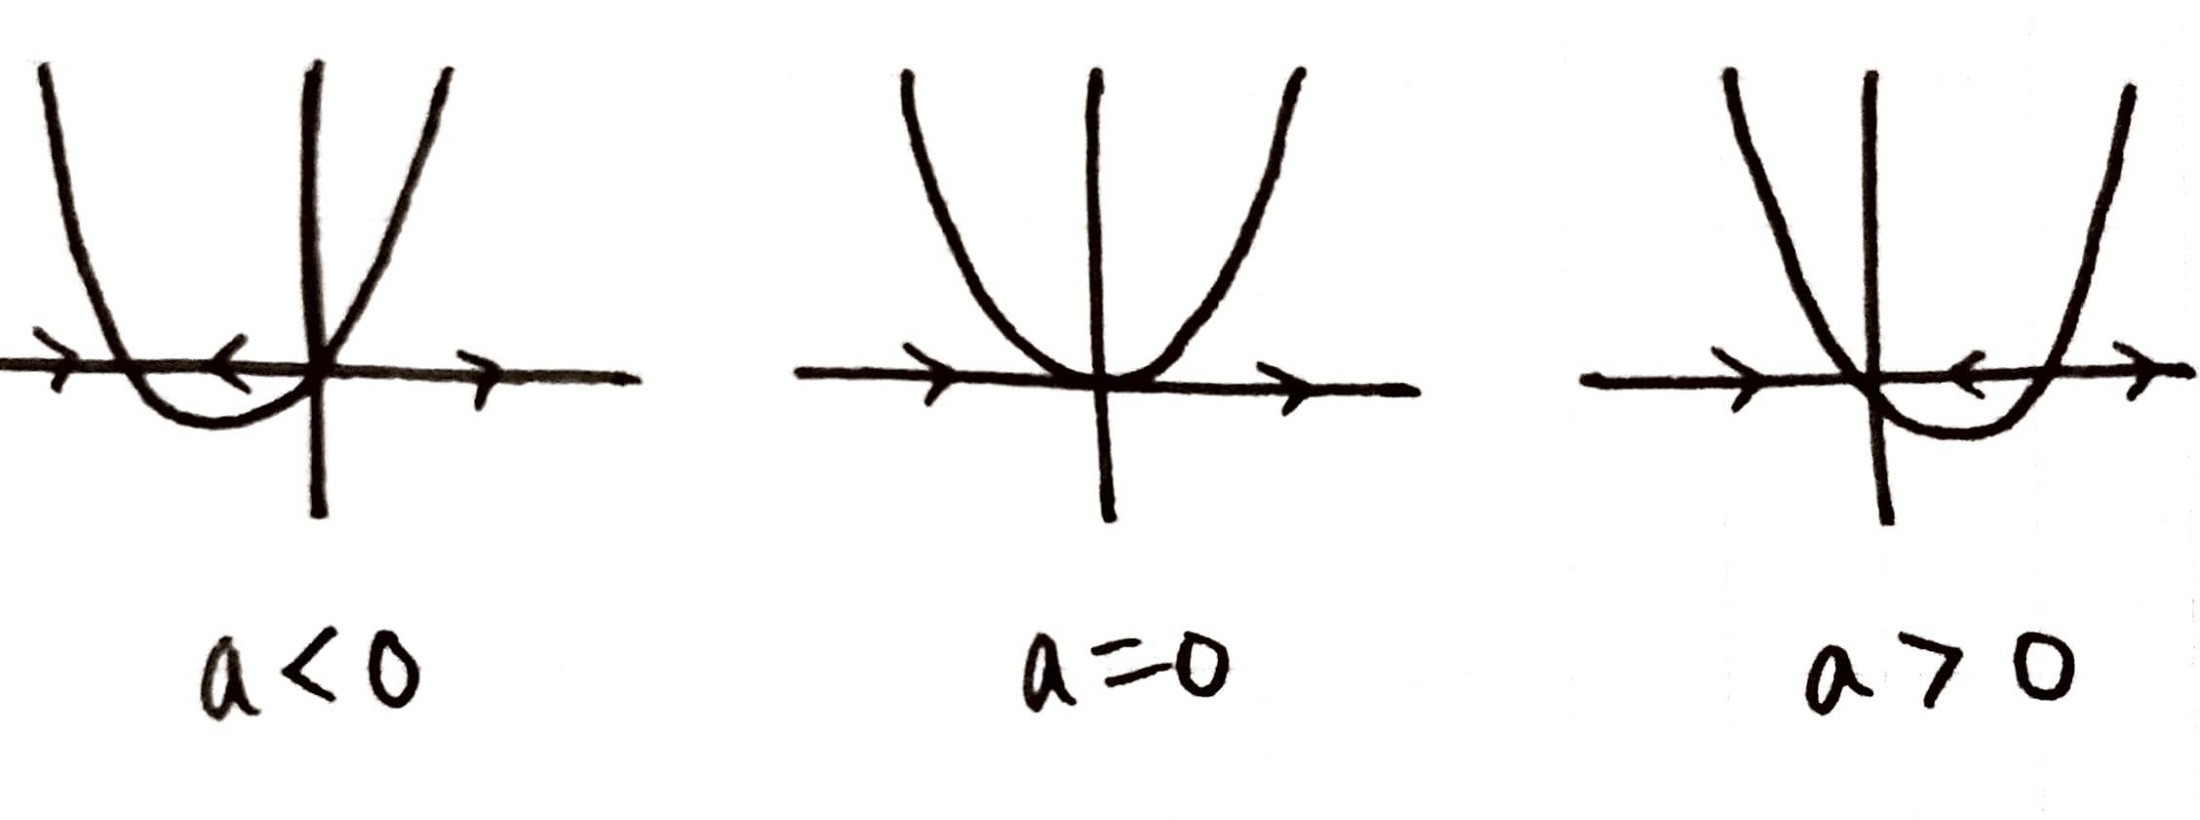
\includegraphics[height=0.2\textwidth]{img/2015S2-1.png}
\end{center}
So, we get the following bifurcation diagram:
\begin{center}
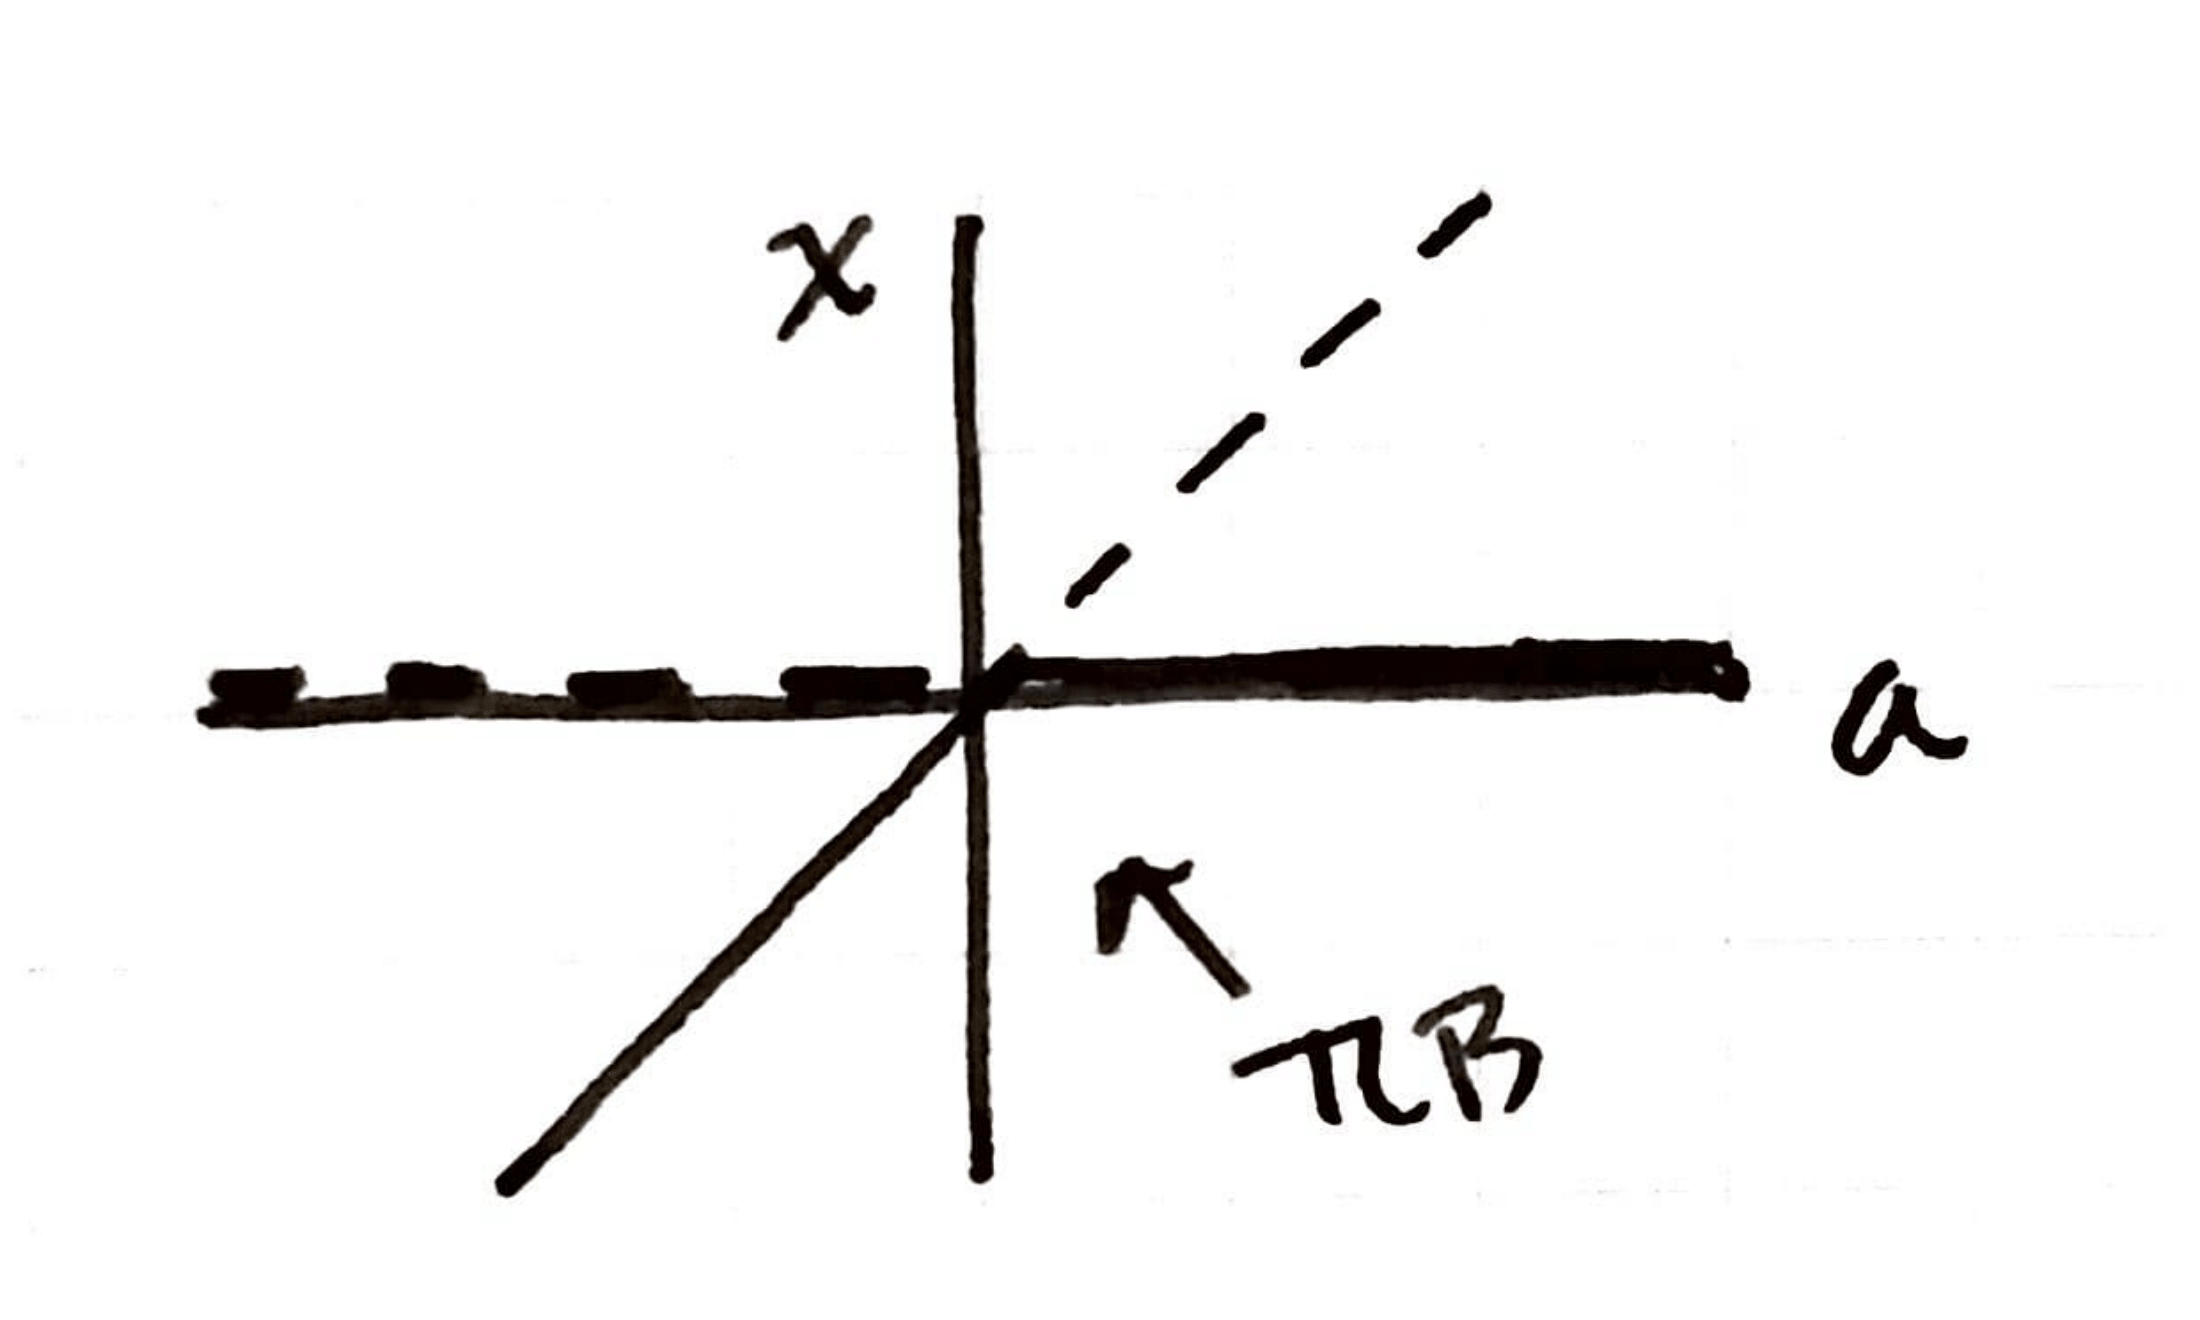
\includegraphics[height=0.2\textwidth]{img/2015S2-2.png}
\end{center}
If $b = \epsilon$, then the graph of $x(x-a) + \epsilon$ looks like the following:
\begin{center}
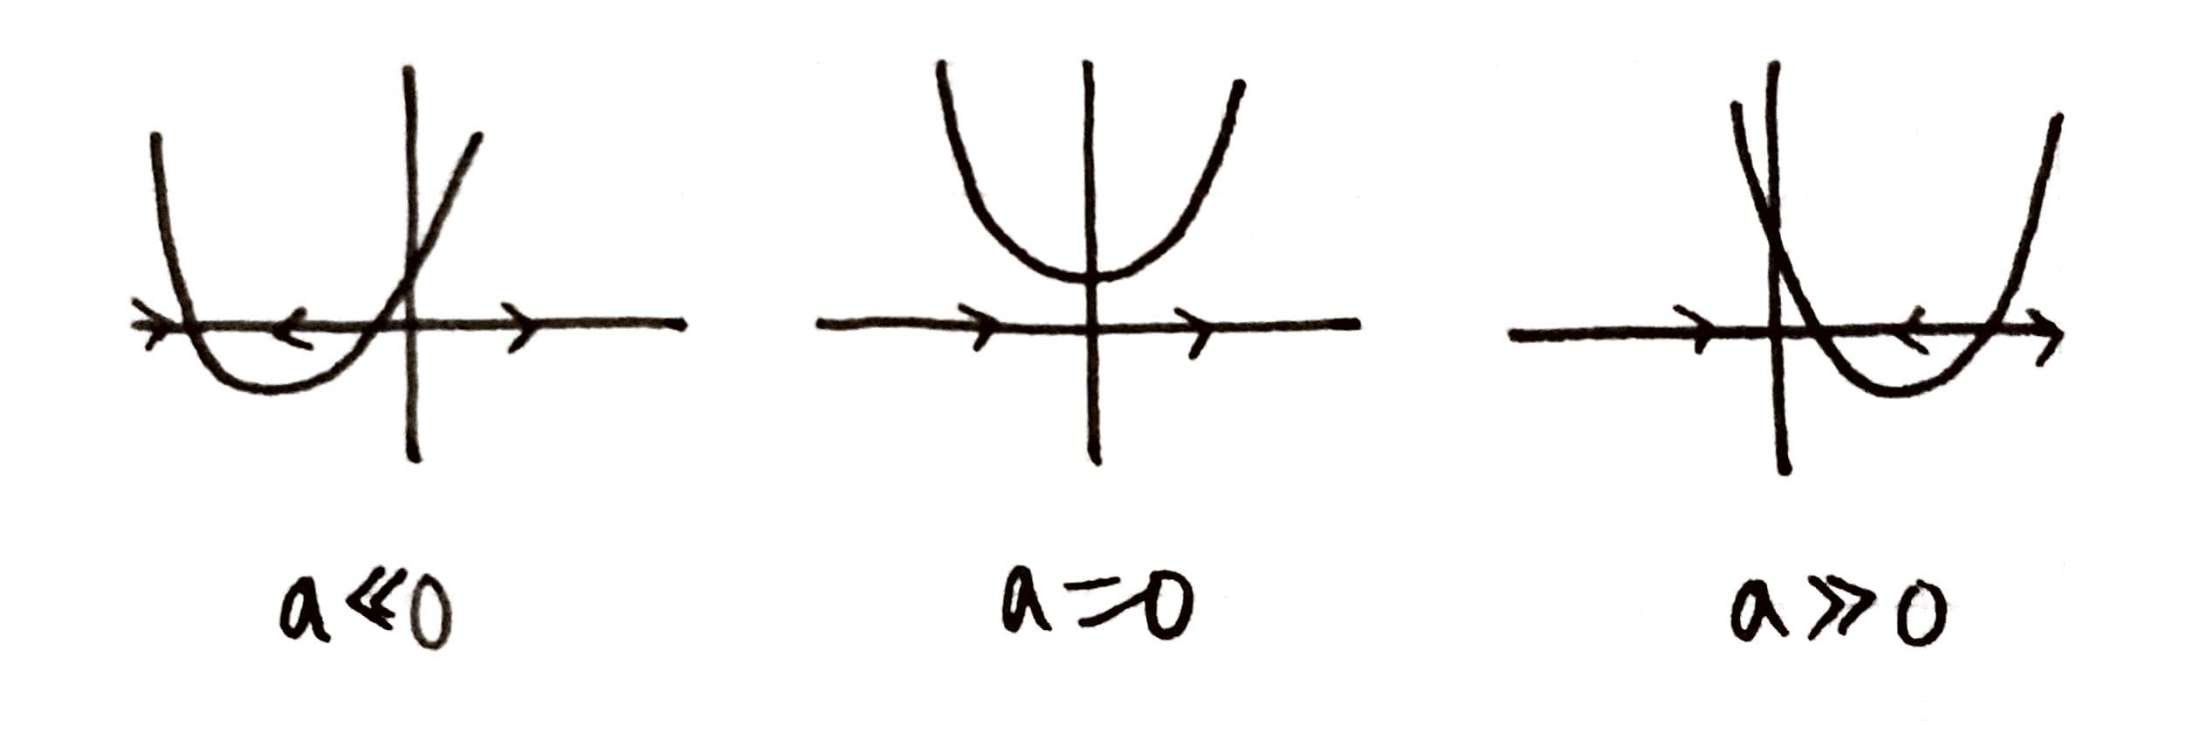
\includegraphics[height=0.2\textwidth]{img/2015S2-3.png}
\end{center}
So, we get the following bifurcation diagram:
\begin{center}
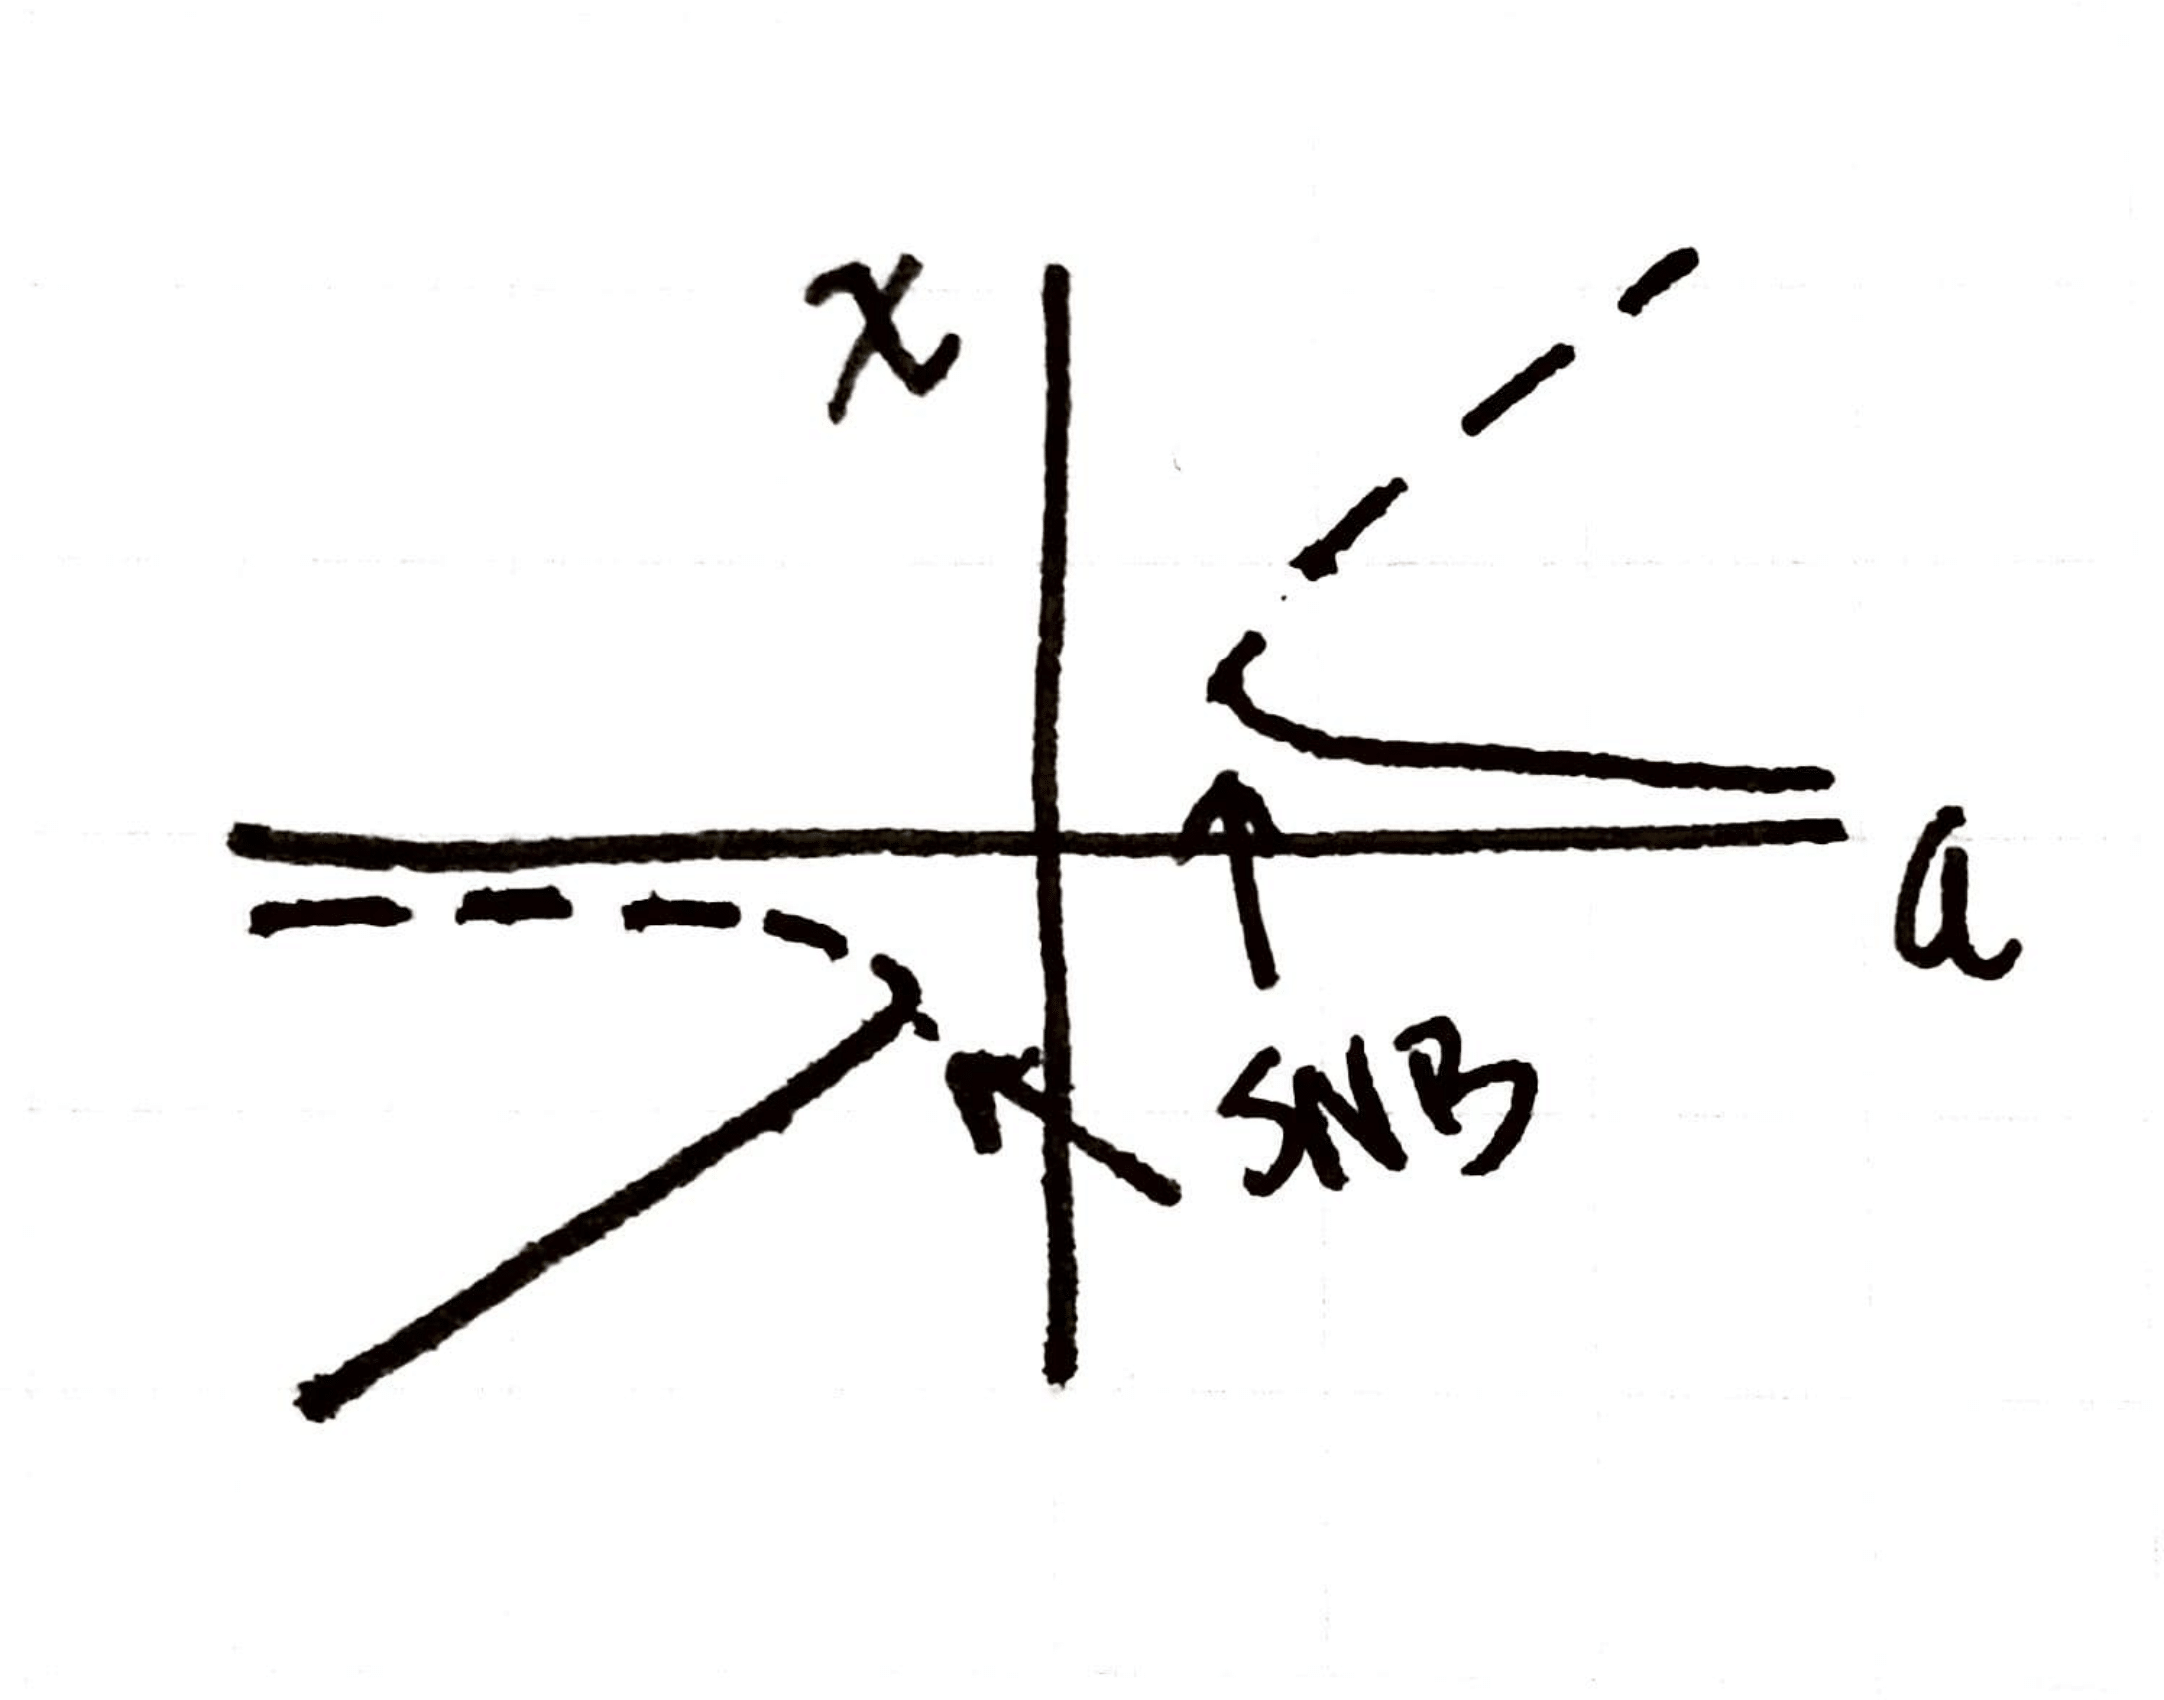
\includegraphics[height=0.2\textwidth]{img/2015S2-4.png}
\end{center}
Finally, if $b = -\epsilon$, then the graph of $x(x-a) - \epsilon$ looks like the following:
\begin{center}
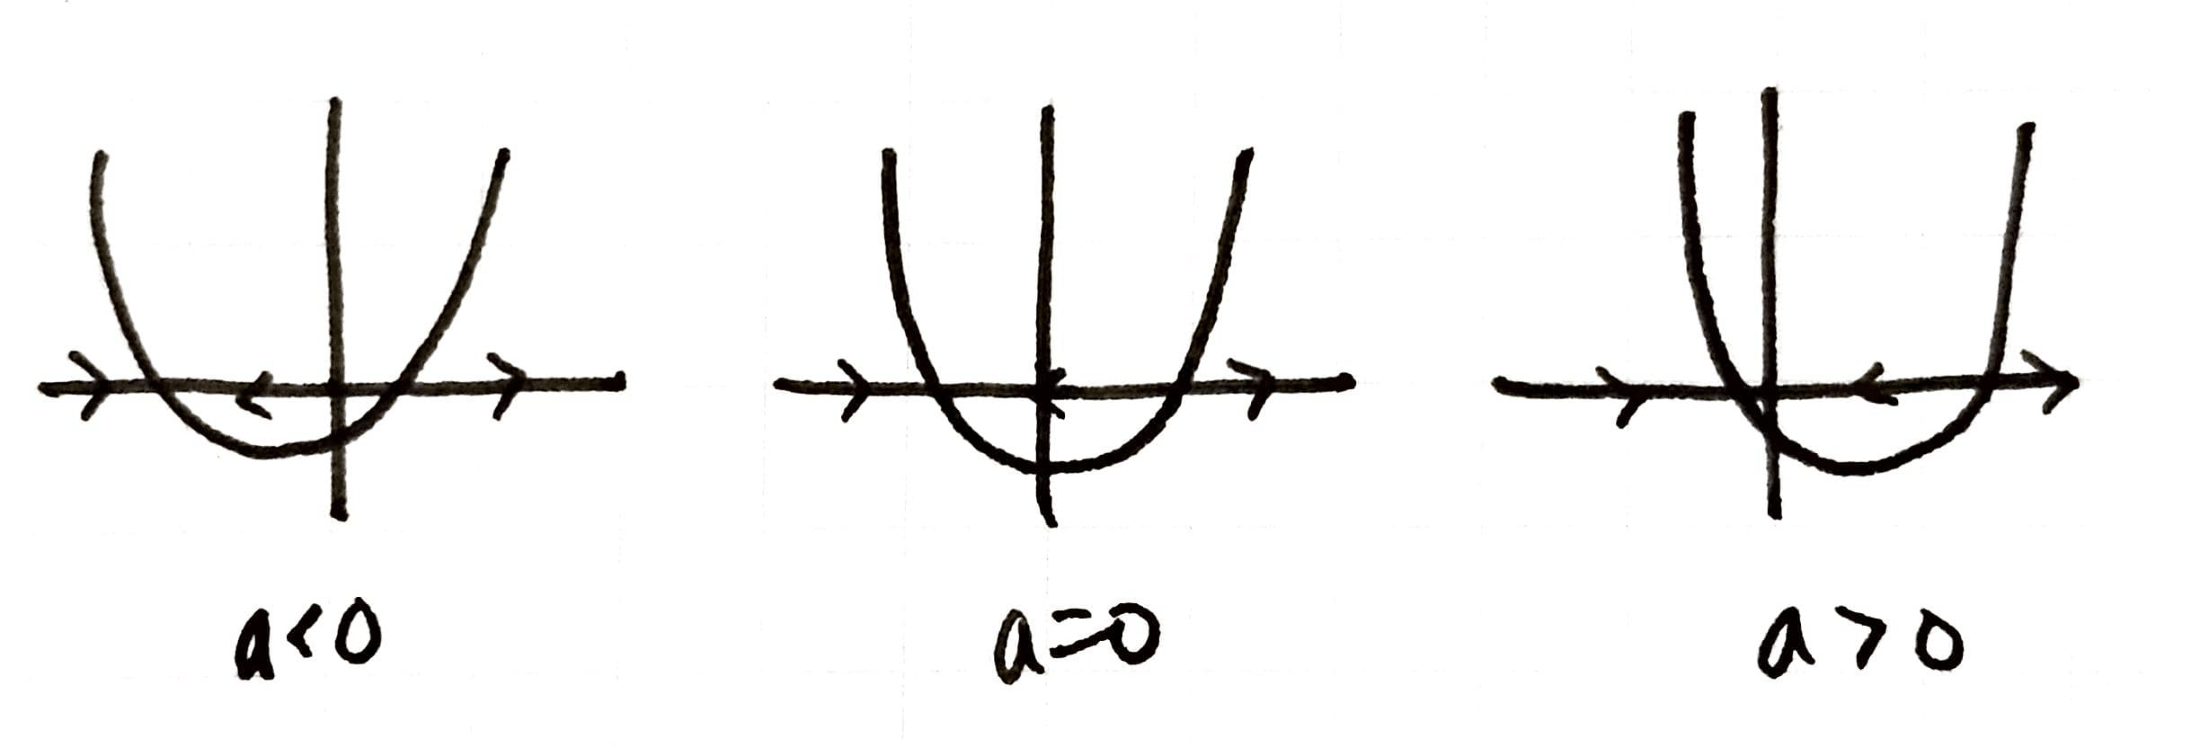
\includegraphics[height=0.2\textwidth]{img/2015S2-5.png}
\end{center}
So, we get the following bifurcation diagram:
\begin{center}
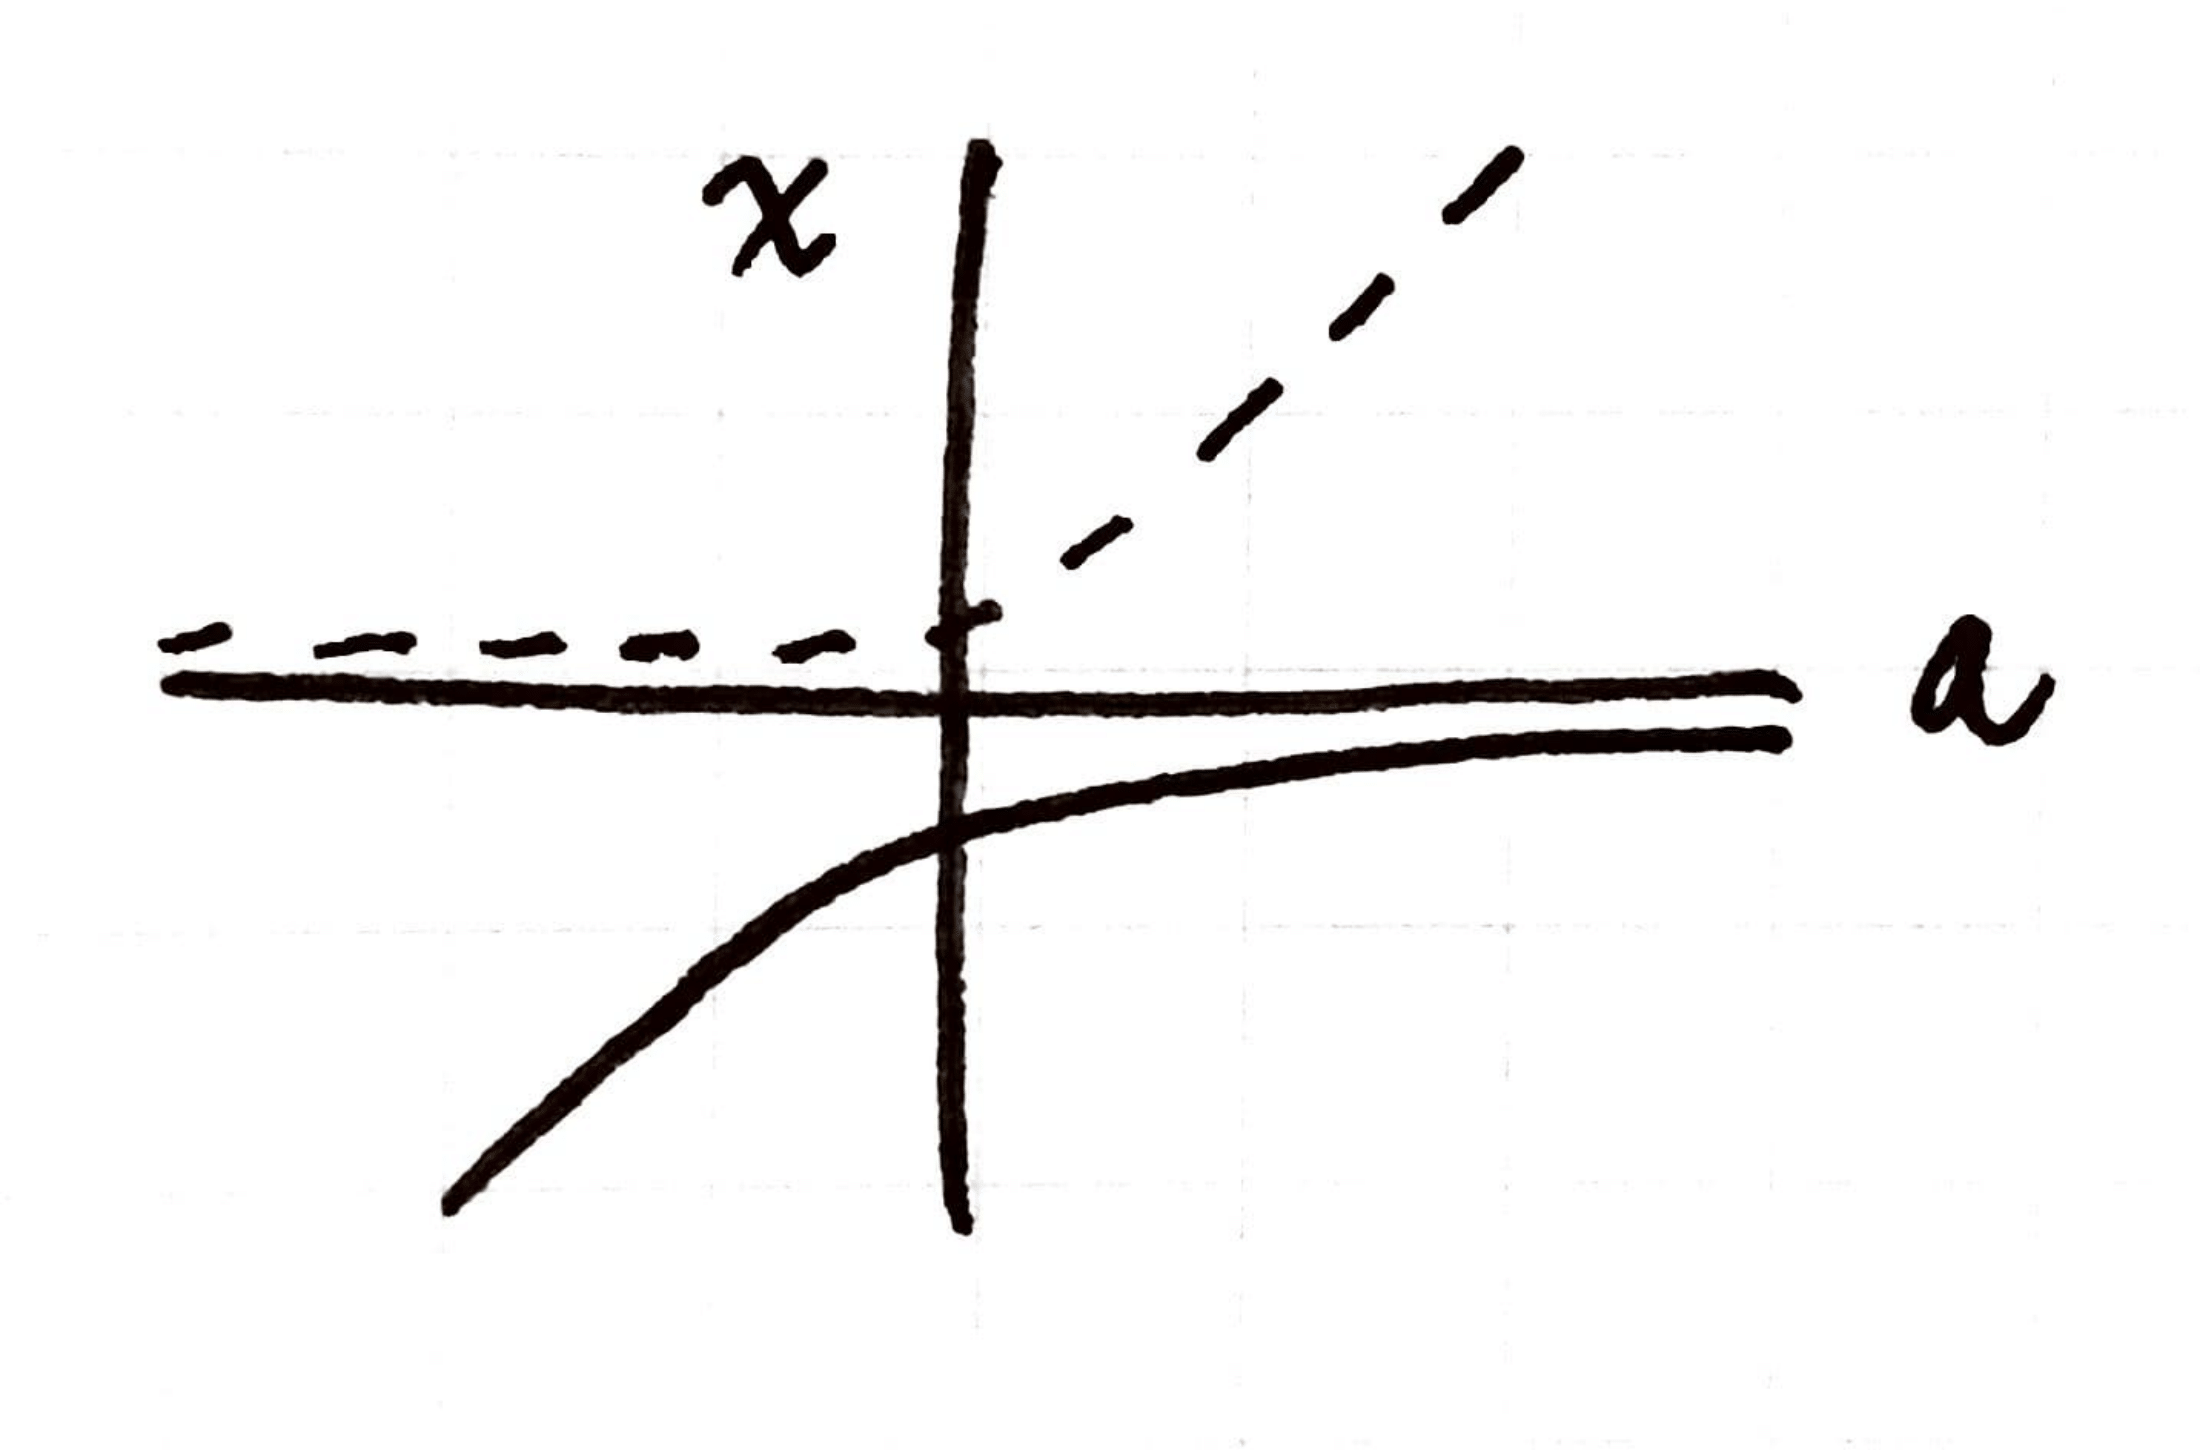
\includegraphics[height=0.2\textwidth]{img/2015S2-6.png}
\end{center}
To sketch our stability diagram, we examine our equilibria in the general case:
\begin{align*}
    x^2 - ax + b &= 0 \so x = \frac{1}{2}\left(a \pm \sqrt{a^2 - 4b}\right)
\end{align*}
So, we have no equilibria when $b > a^2/4$, one equilibrium when $b = a^2/4$, and two otherwise. This gives the following stability diagram:
\begin{center}
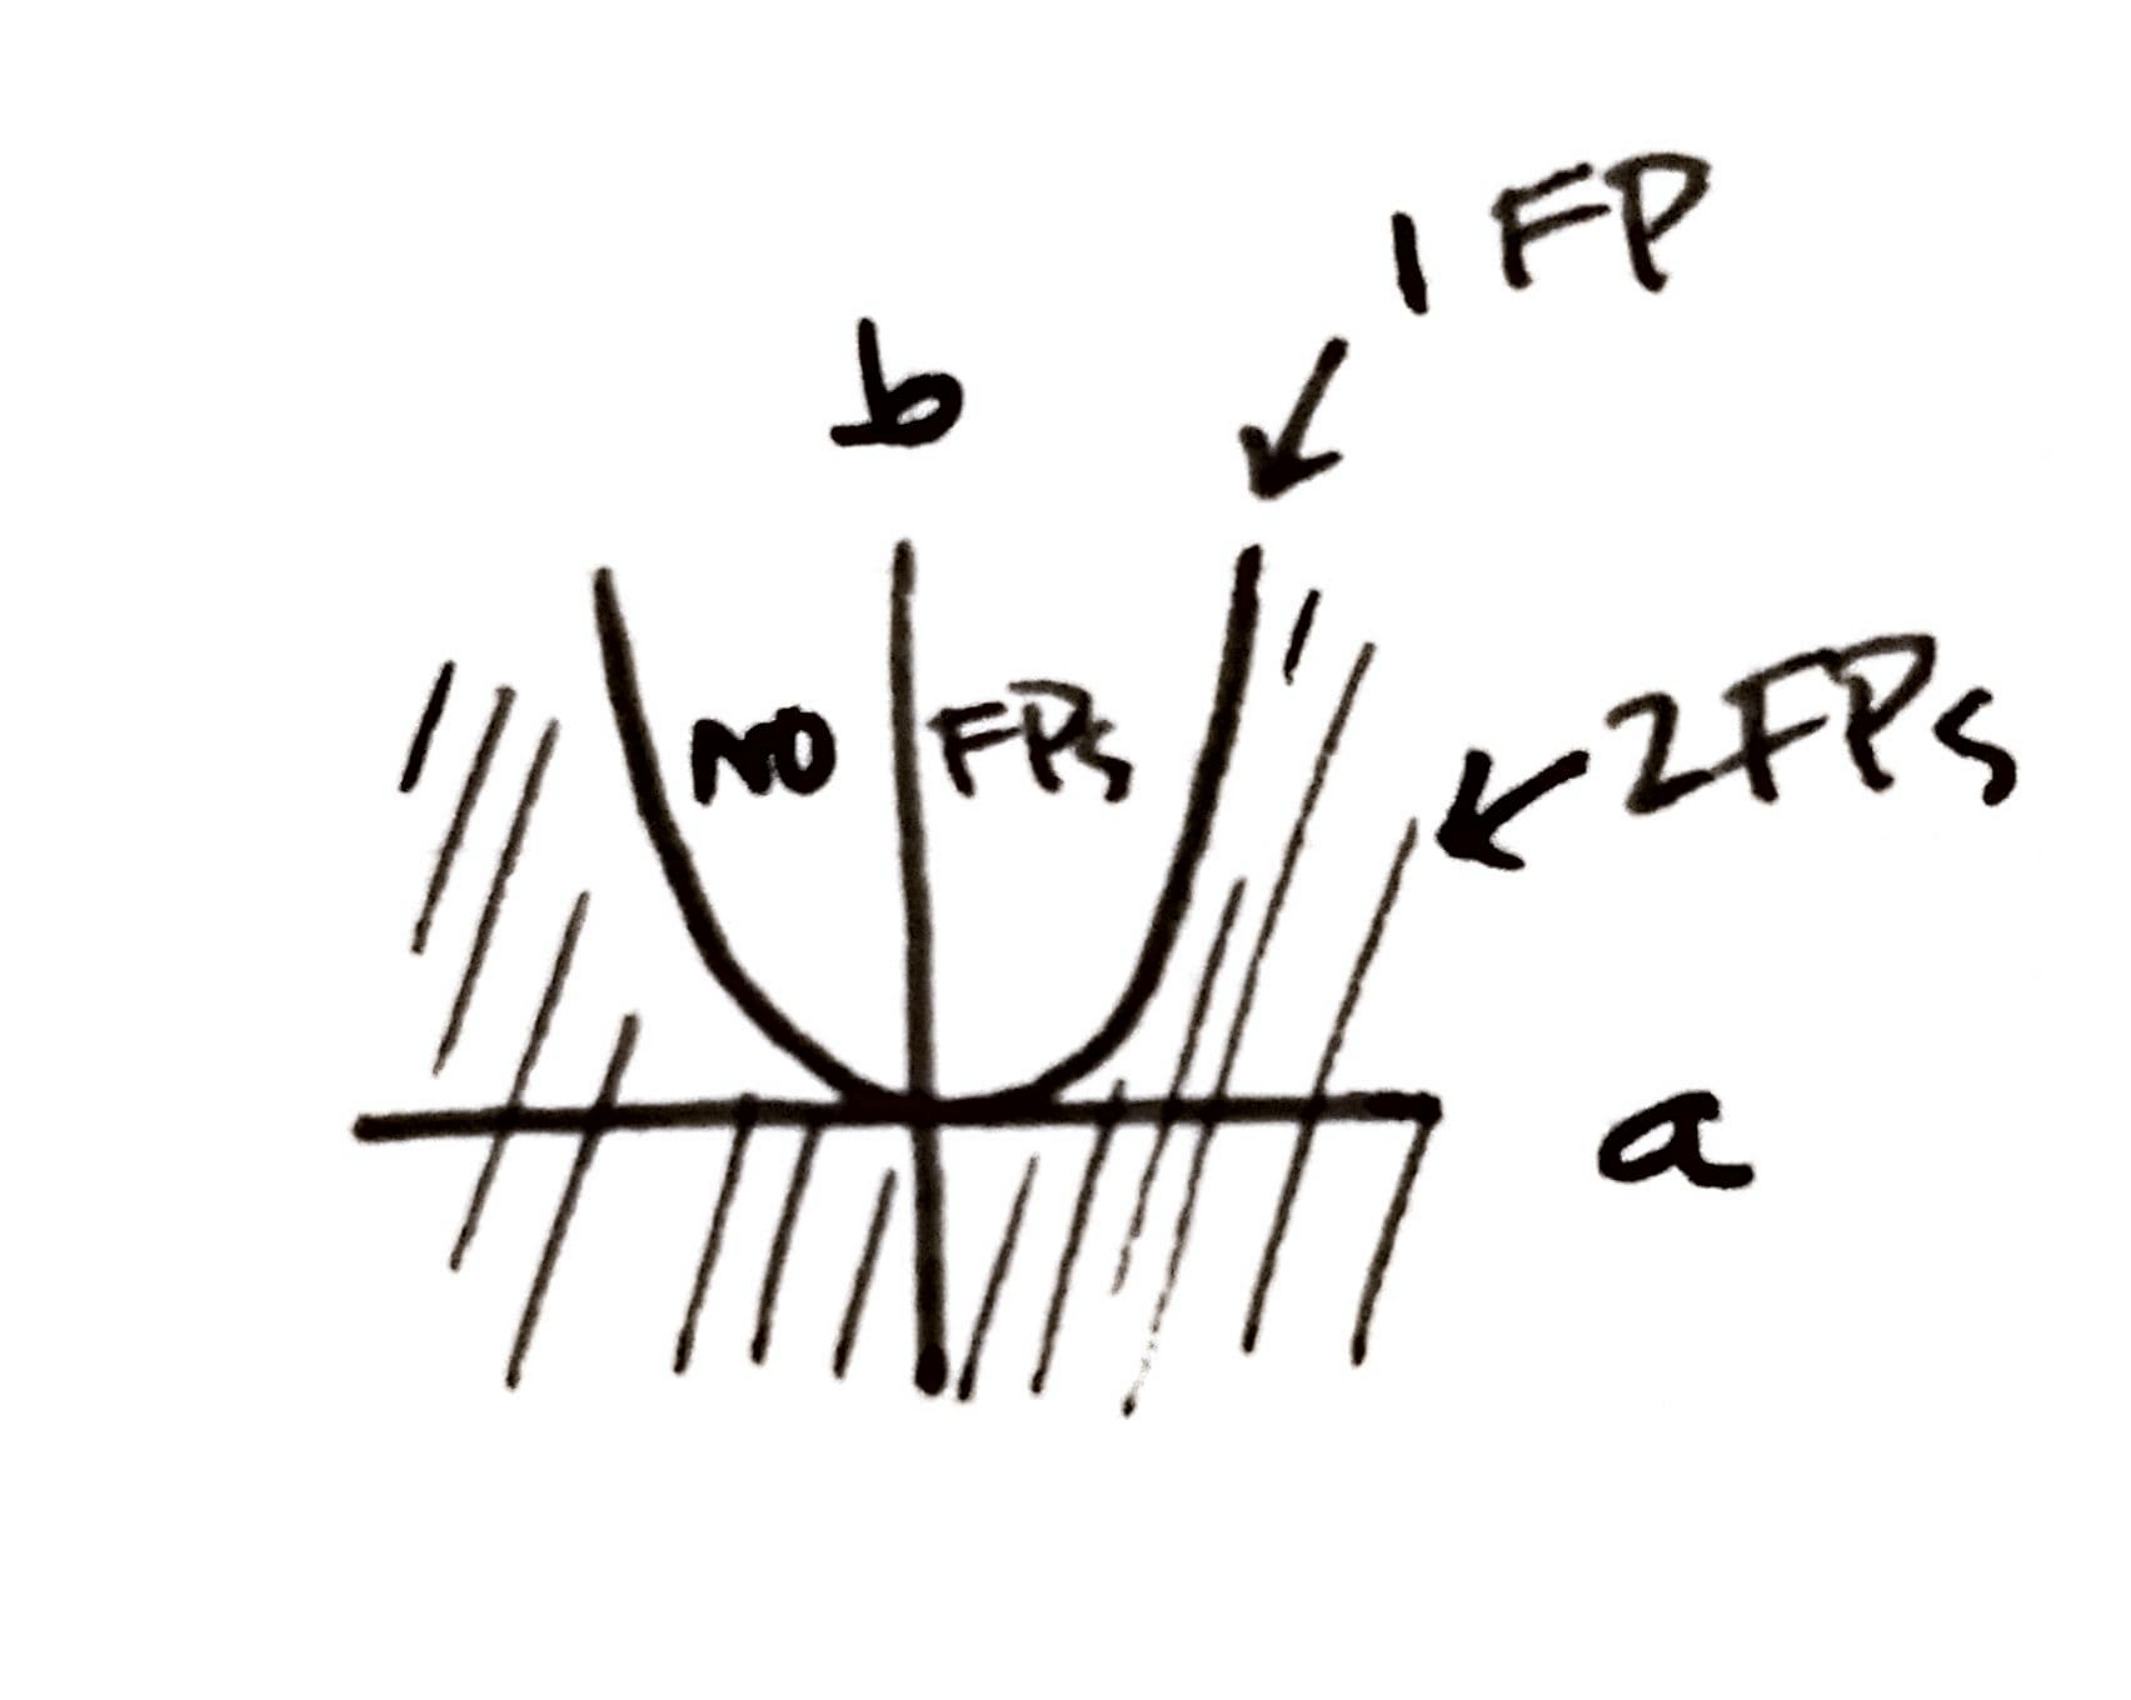
\includegraphics[height=0.3\textwidth]{img/2015S2-7.png}
\end{center}

% \item \begin{qbox}
% Consider waves in a resistant medium that satisfy the problem
% \begin{align*}
% u_{tt} & = u_{xx} - \mu u_t, \qquad \textrm{for}\quad 0 < x < \pi \\
% u_x(0, t) &= 0,\quad u_x(\pi, t) + u(\pi, t) = 0, \\
% u(x, 0) &= \phi(x),\quad u_t(x, 0) = \psi(x),
% \end{align*}
% where $\mu > 0$ is a constant. Write down the Fourier series expansion of the solution.
% \end{qbox}

% \item \begin{qbox} \vspace{-1.5em}
% \begin{itemize}
%     \item[\textbf{(a)}] Show that
%     \[
%     \int_a^x \int_a^s f(t)\,dt\,ds = \int_a^x (x-t)f(t)\,dt
%     \]
%     \item[\textbf{(b)}] Express the linear second order ODE
%     \begin{align*}
%         y'' + \alpha y' + c^2 y &= 0 \\
%         y(0) = 0,\ y'(0) &= 1
%     \end{align*}
%     as an integral equation of the form 
%     \[
%     y(x) = h(x) + \int_0^x K(x, t) y(t)\,dt.
%     \]
%     Determine the functions $h(x)$ and $K(x, t)$.
%     \item[\textbf{(c)}] What is the asymptotic behavior of $y$ (as $x \to \infty$) as a function of the sign of $\alpha$?
% \end{itemize}
% \end{qbox}
% \addtocounter{enumi}{2}

% \item \begin{qbox}
% Find the the first two terms in the asymptotic approximation of the integral
% \[
% \int_0^1 e^{x\left[t\left(1-t^2\right)\right]}\,dt
% \]
% in the following two limits: (a) $x \to -\infty$ and (b) $x \to \infty$. (\textit{Hint}. Use two different methods to study the cases (a) and (b).)
% \end{qbox}

% \begin{enumerate}
% \item  We approximate the integral in the limit as $x \to -\infty$.
% \end{enumerate}

% \item \begin{qbox}
% The equation of motion for a pendulum of length $L$ is
% \[
% \frac{d^2\theta}{dt^2} + \frac{g}{L}\sin\theta = 0,
% \]
% where $\theta(t)$ is the angle measured from the downward vertical direction, and $g$ is the acceleration of gravity. For small initial data,
% \[
% \theta(0) = \epsilon \ll 1,\quad 
% \frac{d\theta}{dt}(0) = 0,
% \]
% use the method of multiple scales to calculate the first two terms in the asymptotic expansion (in $\epsilon$) of the frequency of the pendulum. You will need to introduce the slow time scale $T = \epsilon^2t$.
% \end{qbox}


\end{enumerate}

\end{document}